% \documentclass[11pt, paper=a4]{scrartcl}
\documentclass[11pt, paper=a4]{scrbook}
\usepackage[T1]{fontenc}
\usepackage[utf8]{inputenc}
\usepackage{graphicx}
\usepackage{amsmath,amsfonts,amssymb, amsthm}
\usepackage{bm}
\usepackage{graphicx}
\usepackage{color}
\usepackage{rotating}
\usepackage{cite}
\usepackage{textcomp}
\usepackage{lmodern}
\usepackage{color}
\usepackage{chngcntr}
% makes Fig number in the form Fig. <Section-Nr>.number with number being reset after every section (i.e. new blog entry)
\counterwithin{figure}{section}
\counterwithin{equation}{section}
\usepackage{hyperref}
\usepackage{makeidx}
\usepackage{float}
\usepackage{subcaption}
\makeindex

%\usepackage{pstricks}


\setlength{\parindent}{0pt}

\usepackage{tikz}
\usetikzlibrary{arrows,%
                petri,%
                topaths}%
\usepackage{tkz-berge}

\usepackage{todonotes}


\newcommand{\abf}{\mathbf{a}}
\newcommand{\bbf}{\mathbf{b}}
\newcommand{\cbf}{\mathbf{c}}
\newcommand{\dbf}{\mathbf{d}}
\newcommand{\ebf}{\mathbf{e}}
\newcommand{\fbf}{\mathbf{f}}
\newcommand{\gbf}{\mathbf{g}}
\newcommand{\hbf}{\mathbf{h}}
\newcommand{\ibf}{\mathbf{i}}
\newcommand{\jbf}{\mathbf{j}}
\newcommand{\kbf}{\mathbf{k}}
\newcommand{\lbf}{\mathbf{l}}
\newcommand{\mbf}{\mathbf{m}}
\newcommand{\nbf}{\mathbf{n}}
\newcommand{\obf}{\mathbf{o}}
\newcommand{\pbf}{\mathbf{p}}
\newcommand{\qbf}{\mathbf{q}}
\newcommand{\rbf}{\mathbf{r}}
\newcommand{\sbf}{\mathbf{s}}
\newcommand{\tbf}{\mathbf{t}}
\newcommand{\ubf}{\mathbf{u}}
\newcommand{\vbf}{\mathbf{v}}
\newcommand{\wbf}{\mathbf{w}}
\newcommand{\xbf}{\mathbf{x}}
\newcommand{\ybf}{\mathbf{y}}
\newcommand{\zbf}{\mathbf{z}}



\newcommand{\Abf}{\mathbf{A}}
\newcommand{\Bbf}{\mathbf{B}}
\newcommand{\Cbf}{\mathbf{C}}
\newcommand{\Dbf}{\mathbf{D}}
\newcommand{\Ebf}{\mathbf{E}}
\newcommand{\Fbf}{\mathbf{F}}
\newcommand{\Gbf}{\mathbf{G}}
\newcommand{\Hbf}{\mathbf{H}}
\newcommand{\Ibf}{\mathbf{I}}
\newcommand{\Kbf}{\mathbf{K}}
\newcommand{\Lbf}{\mathbf{L}}
\newcommand{\Mbf}{\mathbf{M}}
\newcommand{\Nbf}{\mathbf{N}}
\newcommand{\Obf}{\mathbf{O}}
\newcommand{\Pbf}{\mathbf{P}}
\newcommand{\Rbf}{\mathbf{R}}
\newcommand{\Sbf}{\mathbf{S}}
\newcommand{\Tbf}{\mathbf{T}}
\newcommand{\Ubf}{\mathbf{U}}
\newcommand{\Vbf}{\mathbf{V}}
\newcommand{\Wbf}{\mathbf{W}}
\newcommand{\Xbf}{\mathbf{X}}
\newcommand{\Ybf}{\mathbf{Y}}
\newcommand{\Zbf}{\mathbf{Z}}

\newcommand{\zerobf}{\mathbf{0}}
\newcommand{\onebf}{\mathbf{1}}
\newcommand{\Sigmabf}{\mathbf{\Sigma}}

\newcommand{\Ac}{\mathcal{A}}
\newcommand{\Dc}{\mathcal{D}}
\newcommand{\Ec}{\mathcal{E}}
\newcommand{\Gc}{\mathcal{G}}
\newcommand{\Ic}{\mathcal{I}}
\newcommand{\Nc}{\mathcal{N}}
\newcommand{\CNc}{\mathcal{CN}}
\newcommand{\Oc}{\mathcal{O}}
\newcommand{\Qc}{\mathcal{Q}}
\newcommand{\Cc}{\mathcal{C}}
\newcommand{\Sc}{\mathcal{S}}
\newcommand{\Vc}{\mathcal{V}}
\newcommand{\Zc}{\mathcal{Z}}

\newcommand{\mC}{\mathbb{C}}
\newcommand{\mE}{\mathbb{E}}
\newcommand{\mF}{\mathbb{F}}
\newcommand{\mQ}{\mathbb{Q}}
\newcommand{\mR}{\mathbb{R}}
\newcommand{\mZ}{\mathbb{Z}}

\newcommand{\erf}{\mathrm{erf}}
\newcommand{\Exp}{\mathrm{E}}


\newcommand{\be}{\begin{equation}}
\newcommand{\ee}{\end{equation}}

\newcommand{\bee}{\begin{equation*}}
\newcommand{\eee}{\end{equation*}}


\newcommand{\bea}{\begin{align*}}
\newcommand{\eea}{\end{align*}}



% a command to generate a new diary entry
% parameters: title, date, category
\newcommand{\DiaryEntry}[3]{
  %\pagebreak
  %\vspace*{3mm}
  \section{#1, #2}\index{#3!#1 - #2}
  \vspace*{-3mm}
  \textit{#2 #3}

  \noindent\rule{8cm}{0.5pt}
  \vspace{3mm}
  \label{#2:entry}
}

\newtheorem{definition}{Definition}[section]
\newtheorem{theorem}{Theorem}[section]
\newtheorem{problem}{Problem}[section]


\begin{document}

\title{My Personal Journal}
\author{}
\date{}

\maketitle

\tableofcontents

\printindex

\chapter{Entries}

%\DiaryEntry{Least Squares}{2015-06-26}{Maths}


Derivation of the least-squares expression: Given the system matrix \(\mathbf{A}\) and the observation \(\mathbf{y}\), we seek the \(\mathbf{\hat{x}}\) so that the error \(\mathbf{r} = \mathbf{y} - \mathbf{A} \mathbf{x}\) is minimized.

%\pagebreak

\begin{figure}[htb!]
\centering
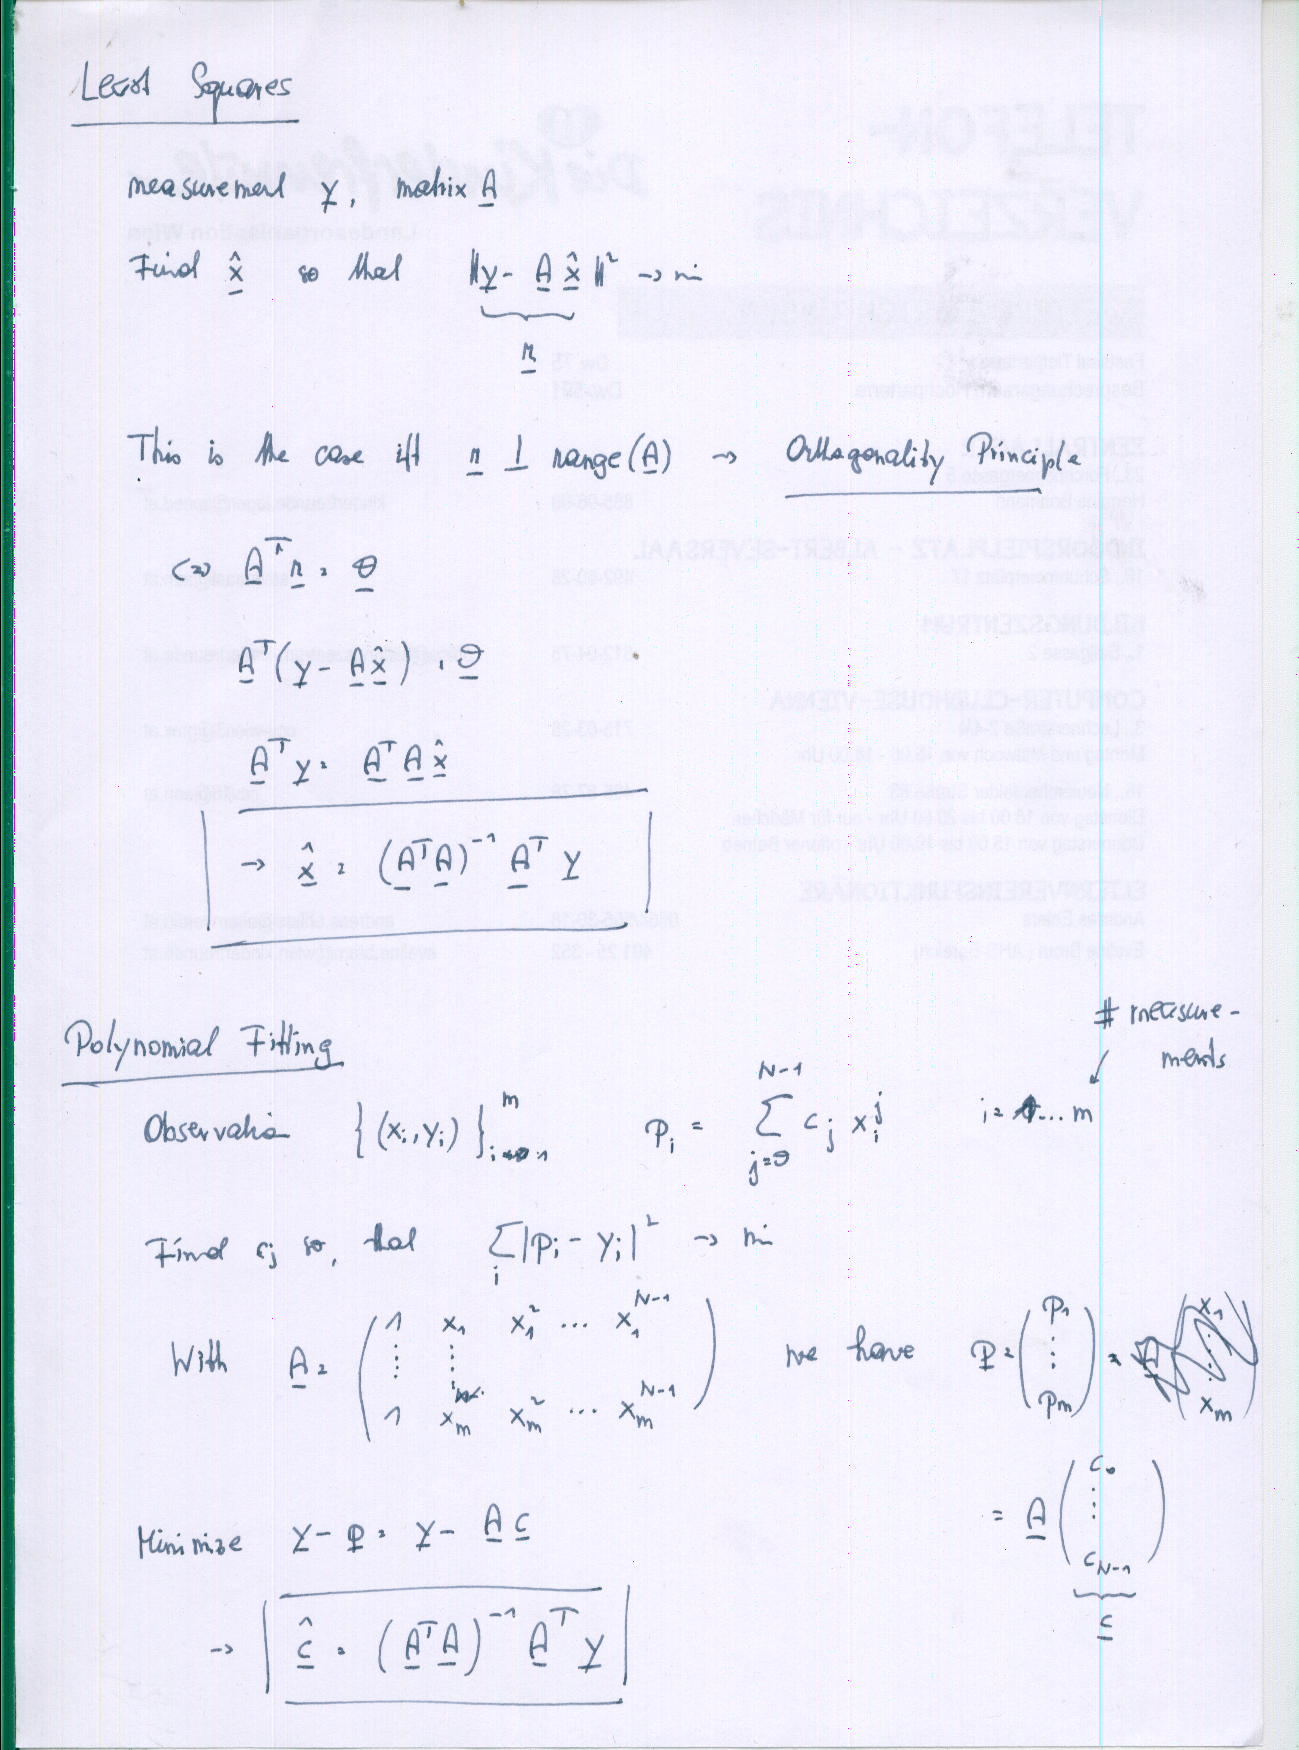
\includegraphics[scale=0.5]{images/least_squares.png}
\caption{Derivation}
\end{figure}

Seen another way, the result \(\mathbf{\hat{x}} = (\mathbf{A}^T \mathbf{A})^{-1} \mathbf{A}^T \mathbf{y}\) is the projection of \(\mathbf{y}\) onto the vector space defined by the columns of \(\mathbf{A}\).

\subsection{Least Squares Example (Julia)}

We consider \(\mathbb{R}^3\) and want to project onto the x-y plane; first we choose the matrix \(\mathbf{A} = [\mathbf{e_1} \mathbf{e_2}]\)

\begin{verbatim}
A=[1 0;0 1;0 0]
inv(A'*A)*A'

2x3 Array{Float64,2}:
1.0  0.0  0.0
0.0  1.0  0.0
\end{verbatim}

The least squares matrix considers only the first two components of any vector it is applied onto =\textgreater{} projection onto x-y plane.

Similarly, nothing (much) changes, if we choose different vectors \(\mathbf{u_1}, \mathbf{u_2}\) for \(\mathbf{A} = [\mathbf{u_1} \mathbf{u_2}]\), as long as they are part of the x-y plane:

\begin{verbatim}
A=[sqrt(2)/2 -sqrt(2)/2;sqrt(2)/2 sqrt(2)/2;0 0]

3x2 Array{Float64,2}:
0.707107  -0.707107
0.707107   0.707107
0.0        0.0     

inv(A'*A)*A'

2x3 Array{Float64,2}:
0.707107  0.707107  0.0
-0.707107  0.707107  0.0
\end{verbatim}

\subsection{Least Squares Polynomial Fitting Example (Julia)}

\subsubsection{No Noise}

We consider \(x_i={-2,-1.2,-0.4,0.4,1.2,2}\) and $y_i=x_i^3$. We least-squares fit three polynoms onto the point set \({x_i,y_i}\) with degree \(N=1\) (a straight line); \(N=3\) (a polynom of the same order as the ``model''), and \(N=6\); i.e. a polynomial with a higher order.

\begin{verbatim}
using Winston

N = 6
srand(1234)

x = linspace(-2,2,N)
y = x.^3

yobs = y

A1 = [x.^0 x.^1]
A3 = [x.^0 x.^1 x.^2 x.^3]
A5 = [x.^0 x.^1 x.^2 x.^3 x.^4 x.^5]


c_hat_1 = inv(A1'*A1)*A1'*yobs
c_hat_3 = inv(A3'*A3)*A3'*yobs
c_hat_5 = inv(A5'*A5)*A5'*yobs

plot(x,yobs,"-rx", x,A1*c_hat_1,"ob", x,A3*c_hat_3,"og", x,A5*c_hat_5,"oy")
savefig("ls_polyfit.pdf")
\end{verbatim}

The following plot shows the results for these different degrees. The observed data is shown in red with circles. The polynomial with $N=1$ (blue circles) gives a bad fit; both $N=3$ (green circles) and $N = 6$ (yellow pluses) yield a pefect match.

\begin{figure}[htb!]
\centering
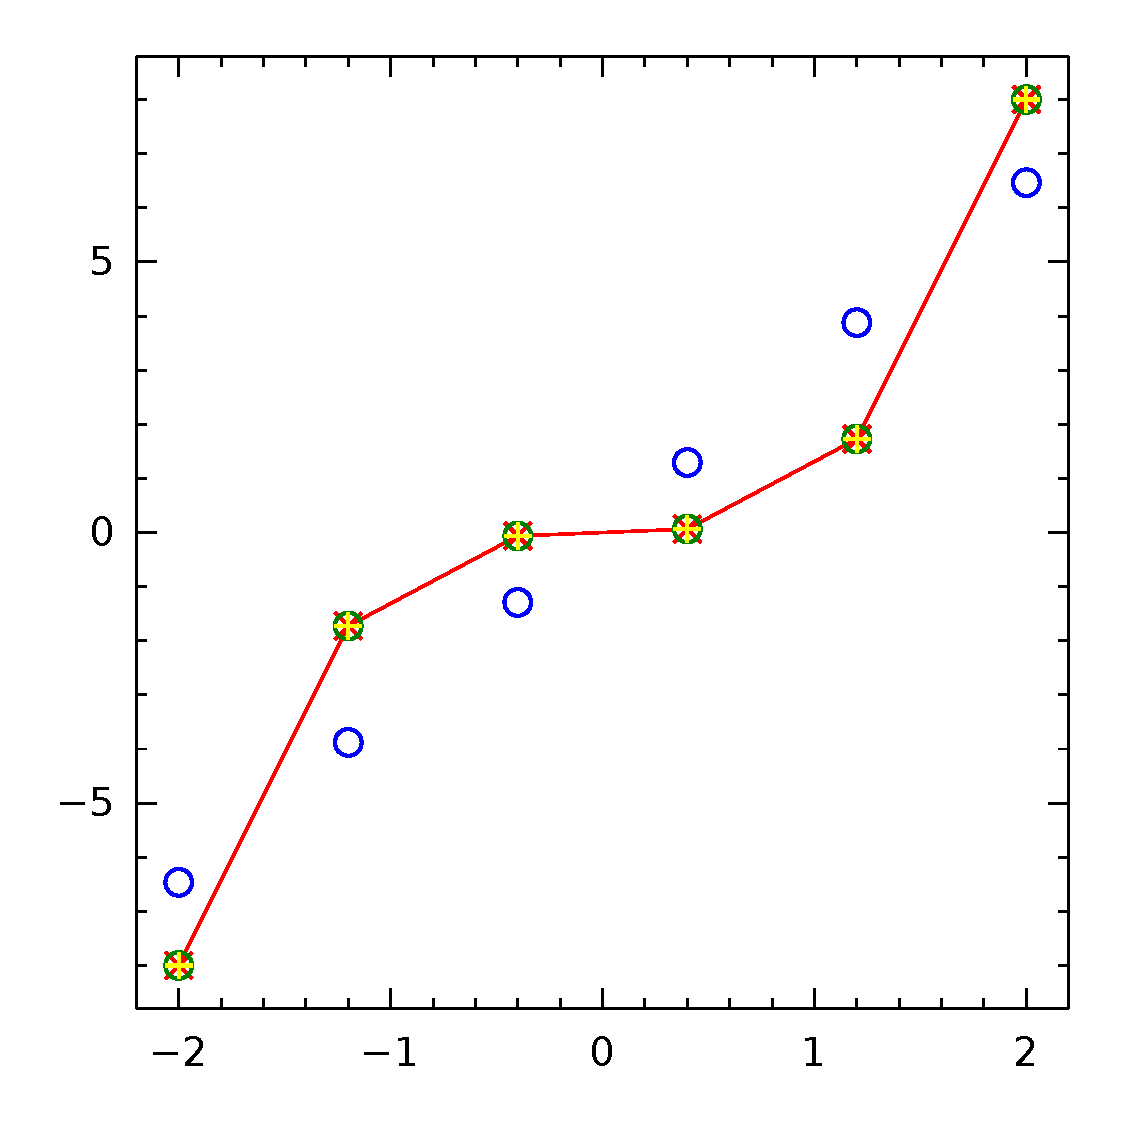
\includegraphics[scale=0.5]{images/ls_polyfit_no_noise.pdf}
\caption{Approximation of noise-free observation with polynomials of degree 1, degree 3, and degree 6, respectively.}
\end{figure}

The coefficient values are as follows

\begin{verbatim}
c_hat_3
4-element Array{Float64,1}:
 0.0       
 1.9984e-15
 0.0       
 1.0

c_hat_5
6-element Array{Float64,1}:
 0.0        
 4.59077e-14
 1.11022e-16
 1.0        
 0.0        
 2.89768e-14

\end{verbatim}

That is, they perfectly match the polynomial $x^3$.


\subsubsection{Measurement with Noise}

Things become different, when the observations are noisy; i.e. $y_i=x_i^3 + w_i$ with the $w_i$ some random Gaussian noise having variance $1$.

The plot below shows the results in this case. It can be seen that the polynomial $N=3$ is now an imperfect match while the polynomial with $N=6$ still has a perfect match: A polynomial of degree $6$ can perfectly match a sequence of $6$ datapoints.


\begin{figure}[htb!]
\centering
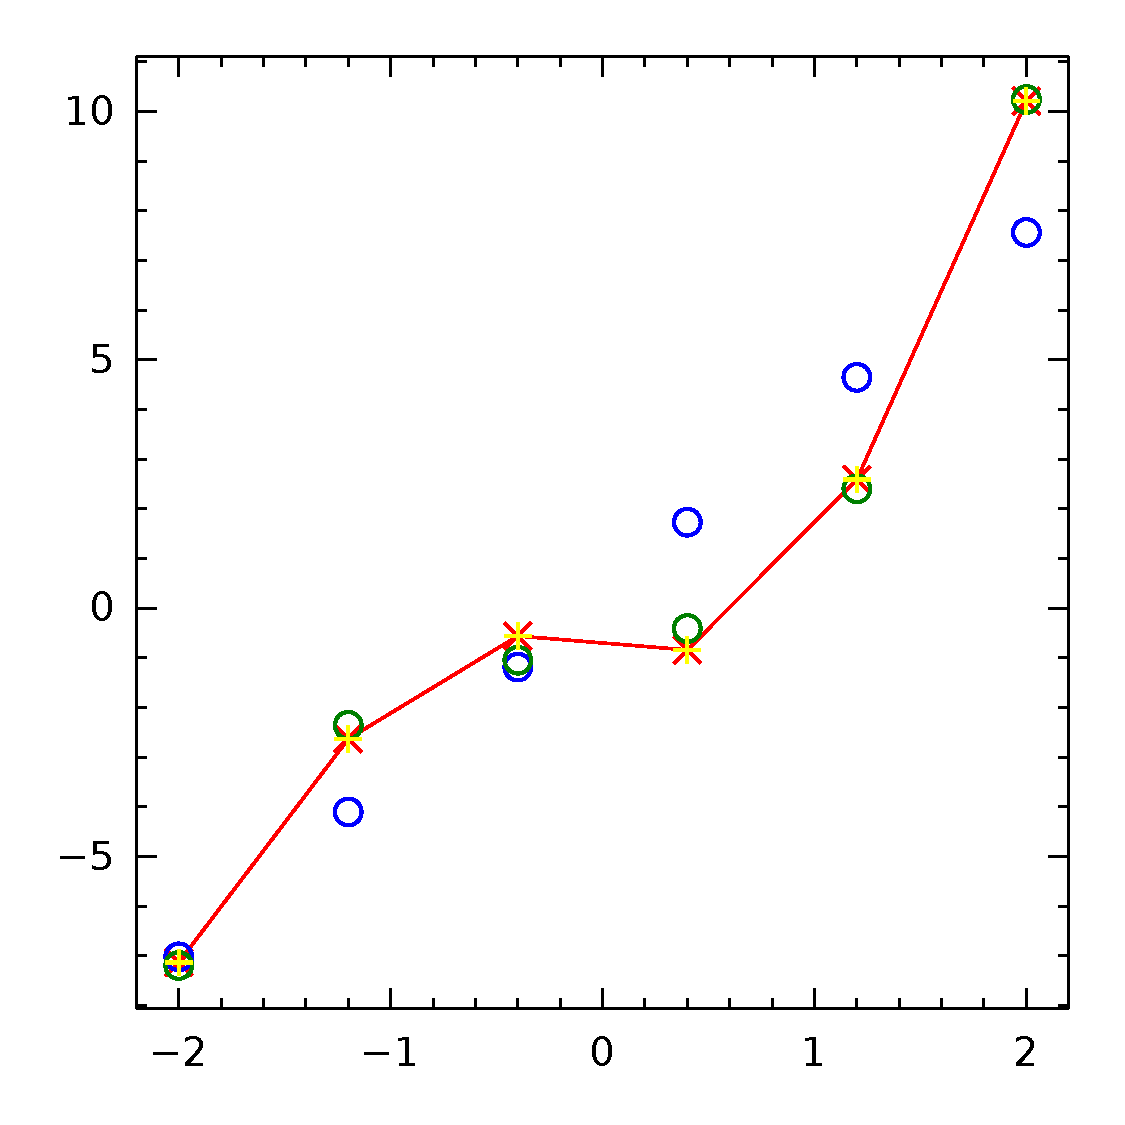
\includegraphics[scale=0.5]{images/ls_polyfit_with_noise.pdf}
\caption{Approximation of noise observation with polynomials of degree 1, degree 3, and degree 6, respectively.}
\end{figure}

%\DiaryEntry{Programming Languages}{2015-06-27}{Programming}

\subsection{Tasks}\label{tasks}

\begin{enumerate}
\def\labelenumi{\arabic{enumi}.}
\item
  Numerical stuff (lin. alg., (statistical)signal progessing,
  plotting\ldots{})
\item
  Scripting language for simple, day-to-day stuff
\item
  Gui development; i.e.~Qucs complexity level
\item
  something non-standard, supporting advanced concepts; e.g.~functional
  programming, macros, actors\ldots{}
\item
  something for web applications(?)
\end{enumerate}

\subsection{Languages}\label{languages}

\subsubsection{Julia}\label{julia}

Advantages: Modern, performant. Vector / matrix\ldots{} support ootb. A
language for scientific computing. Quite vibrant ecosystem but not as
complete as Python -\textgreater{} use PyCall.

\subsubsection{Python}\label{python}

Nice for everyday scripting, but numerical stuff (numpy) is awkward;
e.g.

\begin{verbatim}
self.current_x_hat = dot(A, x_hat)
self.current_Sigma = dot(A, dot(Sigma, A.T)) + Q
\end{verbatim}

Vectors are supported, but matrices are not really integrated into the
language. A general purpose language with support for scientific
computing (see Julia). Julia offers with PyCall a nice way to tap into
the Python scientific ecosystem.

\subsubsection{C\# / Mono + Winforms}\label{c-mono-winforms}

The ``classical'' way to go; cross-platform, lots of documentation
available (Windows World), sufficiently ``modern'' (more than Java).

\subsubsection{Scheme / Racket}\label{scheme-racket}

Seems to be sufficiently close to ``classical LISP books'' (SICP, The
little Schemer\ldots{}) to use it; nice IDE and nice library ecosystem.

\subsubsection{Ruby}\label{ruby}

Perfect for the few web apps I do (e.g.~in contrast to Django). In
addition, maybe it can replace Python as everyday scripting language.
Need to check ecosystem and compare with Python (main competitor).
Nicer/cleaner syntax/structure than Python in any case; e.g.

Python:

\begin{verbatim}
x = [1,4,3,6]
len(x)
but: x.sort() is a method which does in-place modification!
\end{verbatim}

Ruby

\begin{verbatim}
x = [1,4,3,6]
x.size
x.sort returns a sorted list; no in-place modification!
x.sort! sorts in-place
\end{verbatim}

\subsubsection{C++ / Qt}\label{c-qt}

Qt is a quite complete framework; so C++ with Qt is not ``really'' C++.
Nevertheless, too cumbersome and replaced by C\# / Mono with WinForms.

\subsubsection{Java / Swing}\label{java-swing}

Java is enterprise, but Swing is a bit old =\textgreater{} C\# / Mono +
WinForms is more modern.

\subsubsection{Scala}\label{scala}

Coming up as something new. Uses the JVM =\textgreater{} large
ecosystem. Sufficiently modern / functional / cool. Not overly hyped and
not so weird as e.g.~Haskell.

\subsubsection{Rust}\label{rust}

Nope - I don't think it introduces new concepts, but tries to be a
better (safer) C/C++. However, for all microcontroller/low-level system
stuff, there is C. No need for another Baustelle.

%\section{Interesting Stuff to Read}


\subsection{Papers}

\begin{itemize}

	\item \href{files/Ask HN_ What is the most mind blowing book you've ever read_ _ Hacker News.pdf}{Ask HN: What is the most mind blowing book you've ever read?}

	\item \href{files/Ask HN_ What books have made the biggest impact on your mental models_ _ Hacker News.pdf}{Ask HN: What books have made the biggest impact on your mental models?}

\end{itemize}
	
\subsubsection{Maths}

\begin{itemize}

	\item \href{http://math.stackexchange.com/questions/765198/some-users-are-mind-bogglingly-skilled-at-integration-how-did-they-get-there/1063528\#1063528}{Integration
	Skills}; Special Highlight: \href{http://faculty.swosu.edu/michael.dougherty/book/chapter07.pdf}{Advanced
	Integration Techniques}

	\item arXiv Articles:

	\begin{itemize}
		\item \href{http://arxiv.org/abs/1503.09060}{A Tutorial Introduction to
			the Lambda Calculus}
		\item \href{http://arxiv.org/abs/1503.00875}{Topologies and all that -- A
			Tutorial}
		\item \href{http://arxiv.org/abs/1506.00982}{Game Theory for Signal
			Processing in Networks}
		\item \href{http://arxiv.org/abs/0711.0189}{A Tutorial on Spectral
			Clustering}
	\end{itemize}

	\item \href{http://www.sigplan.org/Newsletters/CACM/Papers/}{SigPlan - CACM Papers}

	\item \href{https://pomax.github.io/bezierinfo/}{A Primer on Bezier Curves}

	\item \href{http://www.jamestanton.com/?category_name=puzzles}{Think Puzzles and Think Cool Math}

	\item \href{dice1.pdf}{A Collection of Dice Problems}

	\item \href{https://probabilityandstats.wordpress.com/}{A Blog on
	Probability and Statistics}

	\item  \href{http://www.galois-group.net/g/EN/theory.html}{The Evariste Galois Archive}

\end{itemize}

\subsubsection{Computer Science}

\begin{itemize}
	
	\item \href{files/Ask HN_ What are your favorite scholarly papers_ Why_ _ Hacker News.pdf}{Ask HN:What are your favorite scholarly papers? Why?}
	
	\item \href{https://github.com/papers-we-love/papers-we-love}{Papers we
		love}

	\item \href{files/Ask HN_ What is your favorite CS paper_ _ Hacker News.pdf}{Ask HN: What is your favorite CS paper?}

	\item \href{files/Ask HN_ What language-agnostic programming books should I read_ _ Hacker News.pdf}{Ask HN: What language-agnostic programming books should I read?}

	\item Monad Stuff

	\begin{itemize}
		\item
		\href{http://bartoszmilewski.com/2015/05/11/using-monads-in-c-to-solve-constraints-1-the-list-monad/}{Link1}
		\item
		\href{http://blog.jle.im/entry/unique-sample-drawing-searches-with-list-and-statet}{Link2}
		\item
		\href{http://www.berniepope.id.au/docs/scala_monads.pdf}{Link3}
		\item
		\href{http://james-iry.blogspot.co.at/2007/10/monads-are-elephants-part-3.html}{Link4}
	\end{itemize}

\end{itemize}

\subsection{Books}

\subsubsection{Maths}

\begin{itemize}

	\item \href{http://people.math.gatech.edu/~cain/textbooks/onlinebooks.html}{Online Mathematics Textbooks}

	\item \href{http://wstein.org/ent/}{Elementary Number Theory: Primes, Congruences, and Secrets}
	
	\item \href{http://aurellem.org/thoughts/html/sussman-reading-list.html}{Sussman
  Reading List}; Special highlights:

	\begin{itemize}
		\item Linear Differential Operators, Cornelius Lanczos
		\item Probability: the Logic of Science, E.T. Jaynes
		\item Calculus on Manifolds, Spivak
		\item The Variational Principles of Mechanics, Cornelius Lanczos
	\end{itemize}

	\item \href{http://www.paulgraham.com/onlisptext.html}{On Lisp}

	\item \href{http://lacim.uqam.ca/~plouffe/articles/MasterThesis.pdf}{Generating Functions List}

	\item \href{http://www2.isye.gatech.edu/~nemirovs/Lect_ModConvOpt.pdf}{LECTURES
  ON MODERNCONVEXOPTIMIZATION}

	\item \href{https://news.ycombinator.com/item?id=10783219}{Books you read in 2015}

	\item \href{Handbook of Applied Cryptography - Chapter02.pdf}{Handbook of Applied Cryptography (Mathematical Background)}

	\item Gamma: Exploring Euler's Constant by Julian Havil

	\item Metric Spaces by M. O'Searcoid

	\item Introduction to Projective Geometry (Dover Books on Mathematics) by C. R. Wylie Jr.

	\item Non-Euclidean Geometry by H. S. M. Coxeter

	\item Euclidean and Non-Euclidean Geometries: Development and History 4th Edition by Marvin J. Greenberg

	\item The SIAM 100-digit challenge: A study in high-accuracy Numerical Computing by Folkmar Bornemann et al

	\item Problems in Applied Mathematics by Klamkin

\subsubsection{Computer Science}

	\item  \href{http://arxiv.org/abs/1512.06808}{Game Theory Textbook}

	\item \href{http://cswww.essex.ac.uk/CSP/papers/CP_Handbook-20060315-final.pdf}{Handbook  of Constraint Programming}
	
	\item \href{http://www.hakank.org/constraint_programming_blog/}{Constraint
  Programming Blog}

	\item \href{http://www.staff.science.uu.nl/~gadda001/goodtheorist/index.html}{How to become a GOOD Theoretical Physicist}
  
	\item \href{http://math.stackexchange.com/questions/94827/books-that-every-student-need\%20s-to-go-through}{Books that every student needs to go through}

	\item \href{http://www.squeakland.org/resources/books/readingList.jsp}{Alan Kay's Reading List}

	\item The Annotated Turing: A Guided Tour Through Alan Turing's Historic
Paper on Computability and the Turing Machine by Petzold

	\item \href{https://lispcookbook.github.io/cl-cookbook/}{Common Lisp Handbook}

\subsubsection{Electronics}

	\item Small Signal Audio Design by Douglas Self

\subsubsection{Economy}

	\item Options, Futures, and Other Derivatives, Hull

	\item Trading and Exchanges: Market Microstructure for Practitioners by Larry Harris

\subsubsection{Other}

	\item The Room: A Novel by Jonas Karlsson

	\item The Hero with a Thousand Faces by Campbell

	\item Time and the Soul by Jacob Needleman

	\item Way of the Peaceful Warrior: A Book That Changes Lives by Dan Millman

	\item Wie viel ist genug?: Vom Wachstumswahn zu einer Oekonomie des guten Lebens von Robert Skidelsky \& Edward Skidelsky

	\item Die Schriften von Accra von Paulo Coelho

	\item Die Gluecksformel von Stefan Klein

	\item Critical Thinking, Moore and Parker

	\item Sergeant Bourgogne - with Napoleon's Imperial Guard in the Russian campaign and on the retreat from Moscow 1812 - 13
	
\end{itemize}

\subsubsection{Body and Health}

\begin{itemize}
  \item \href{http://liamrosen.com/fitness.html}{Beginner's Health and Fitness Guide}

  \item \href{http://darebee.com/workouts/black-ops-workout.html}{Black Ops Workout}

\end{itemize}

%\DiaryEntry{CRC Check Codes}{2015-06-28}{Maths}

A good description of CRC codes/checks can be found here
\url{http://www.ross.net/crc/download/crc_v3.txt}

I'm using a generator polynomial \(x^3 + x + 1\) which is equivalent to
\texttt{1011}.

\subsection{Encoding Example}\label{encoding-example}

As an example, consider encoding of the dataword =
\texttt{110100\ 1110\ 1100}. With the choice of the generator polynomial
as above, the CRC check code will have 3 digits, therefore we augment 3
zeros to the dataword. Then we divide the augmented dataword by the
generator polynomial.

\begin{figure}[H]
\centering
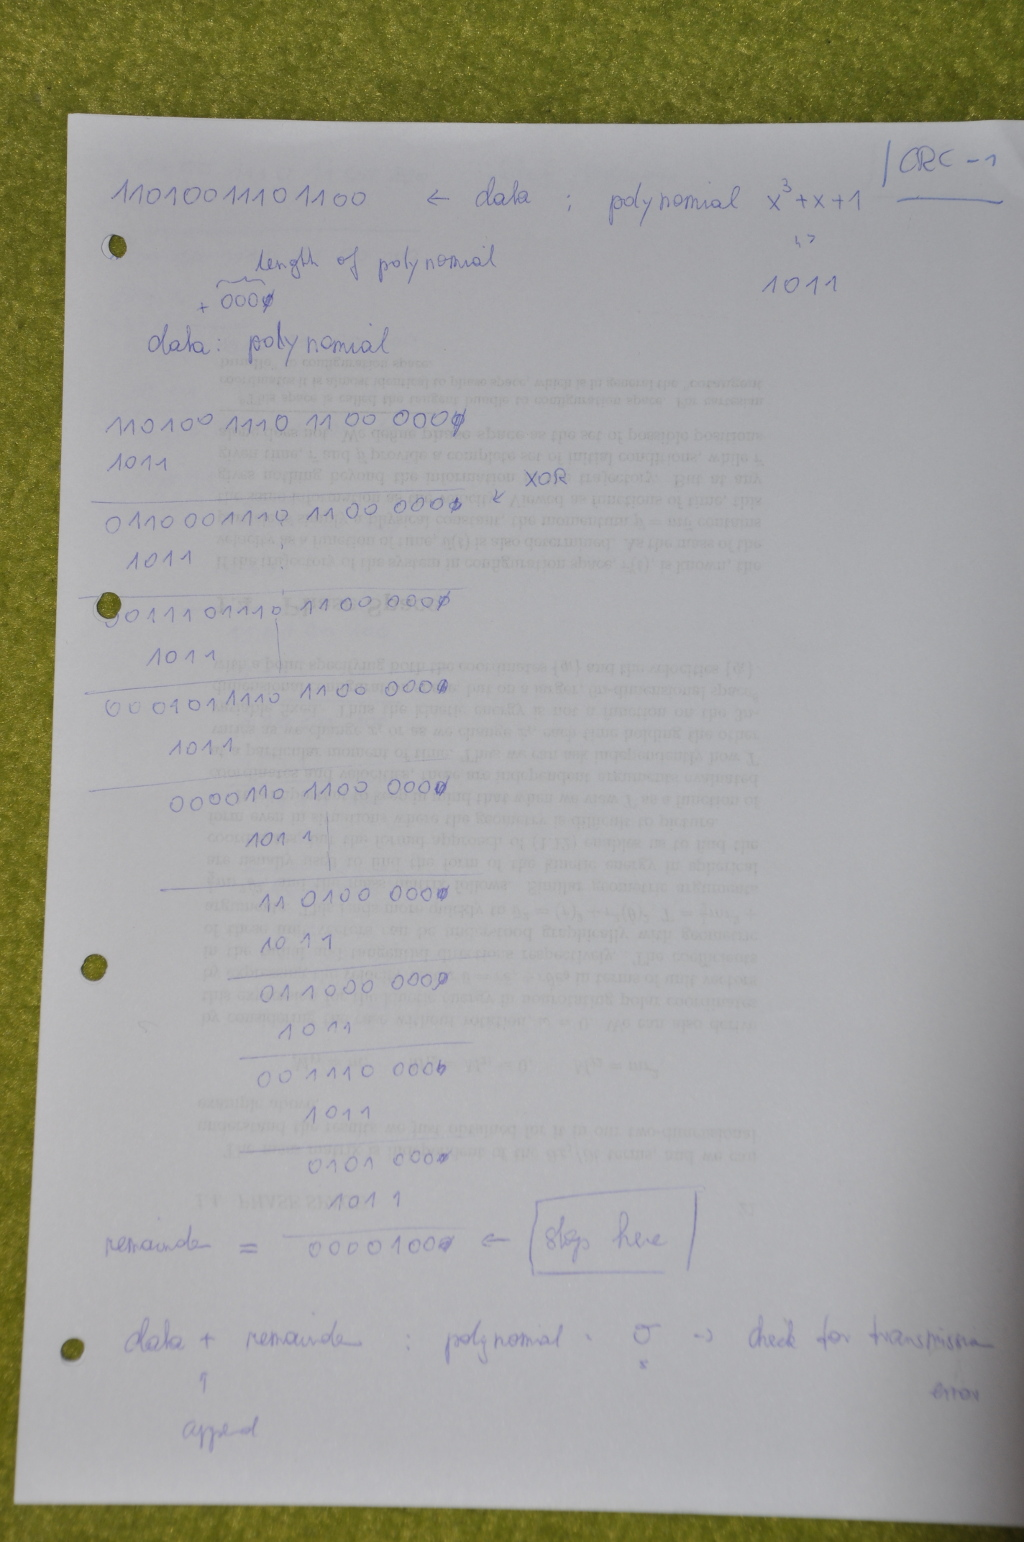
\includegraphics[scale=1.2]{images/DSC_0855_small.JPG}
\end{figure}

Division yields a remainder of \texttt{100} which is the CRC code. We
augment the original dataword with the CRC code to obtain
\texttt{11\ 0100\ 1110\ 1100\ 100}.

\subsection{Decoding Example}\label{decoding-example}

We divide the augmented dataword by the generator polynomial. In case of
no transmission errors, this should yield zero.

\begin{figure}[H]
\centering
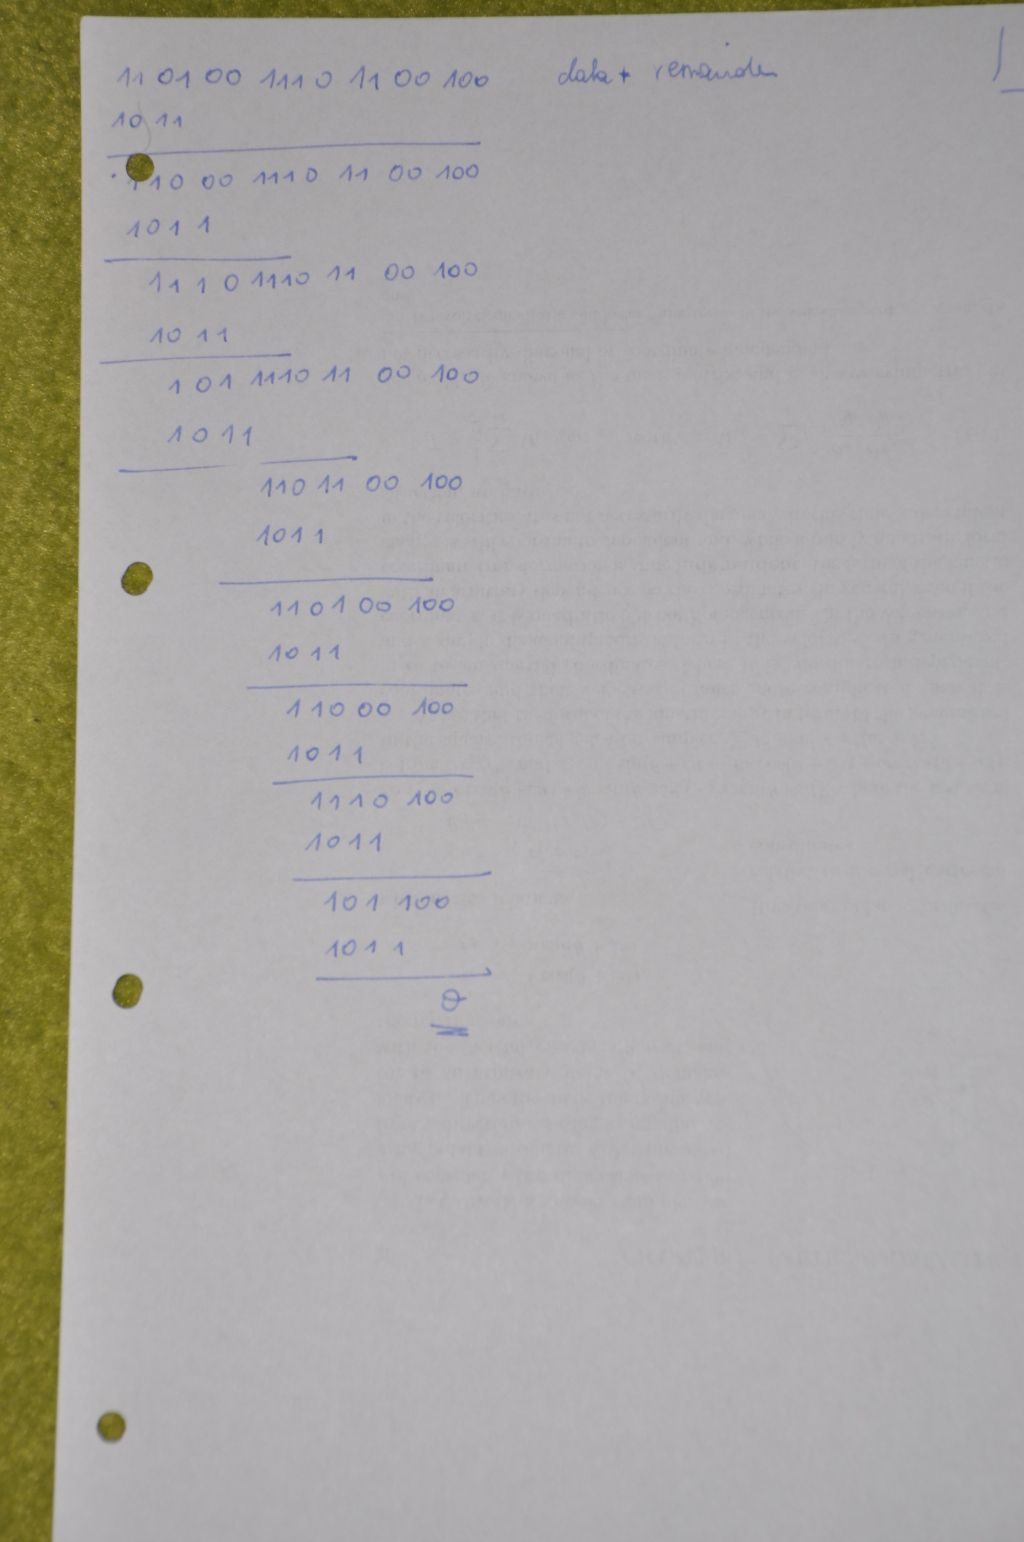
\includegraphics[scale=1.2]{images/DSC_0856_small.JPG}
\end{figure}

\subsection{Julia Example}\label{julia-example}

The (unofficial) Julia Module \texttt{IntModN} provides polynomial
arithmetic over GFs. Below is the example from above solved using this
module.

\begin{verbatim}
include("IntModN.jl")

x=IntModN.X(IntModN.GF2)

w = x^13 + x^12 + x^10 + x^7 + x^6 + x^5 + x^3 + x^2

dw_aug = dw * x^3

# crc code polynomial
p2 = x^3 + x + 1

println(dw_aug)
println(p2)

# divide with remainder; b holds the crc checkword
a, b = IntModN.divrem(dw_aug, p2)

println(a, " ... " , b)

# we finally transmit the dataword augmented with the crc checkword
dw_final = dw_aug + b

# dividing the received dataword by the crc polynomial
c, d = IntModN.divrem(dw_final, p2)

# yields a remainder of zero
println(d)
\end{verbatim}

%\DiaryEntry{Newton Root Finding}{2015-06-28}{Maths}

Find zero(s) for \(f(x)\). The basic idea is to start with a point
\(x_n\) on \(f(x)\) and calculate the tangent \(g(x)\) to the curve at
this point. Find the zero of the tangent \(g(x)\); that's \(x_{n+1}\);
i.e.~the next starting point.

\begin{figure}[hbt!]
\centering
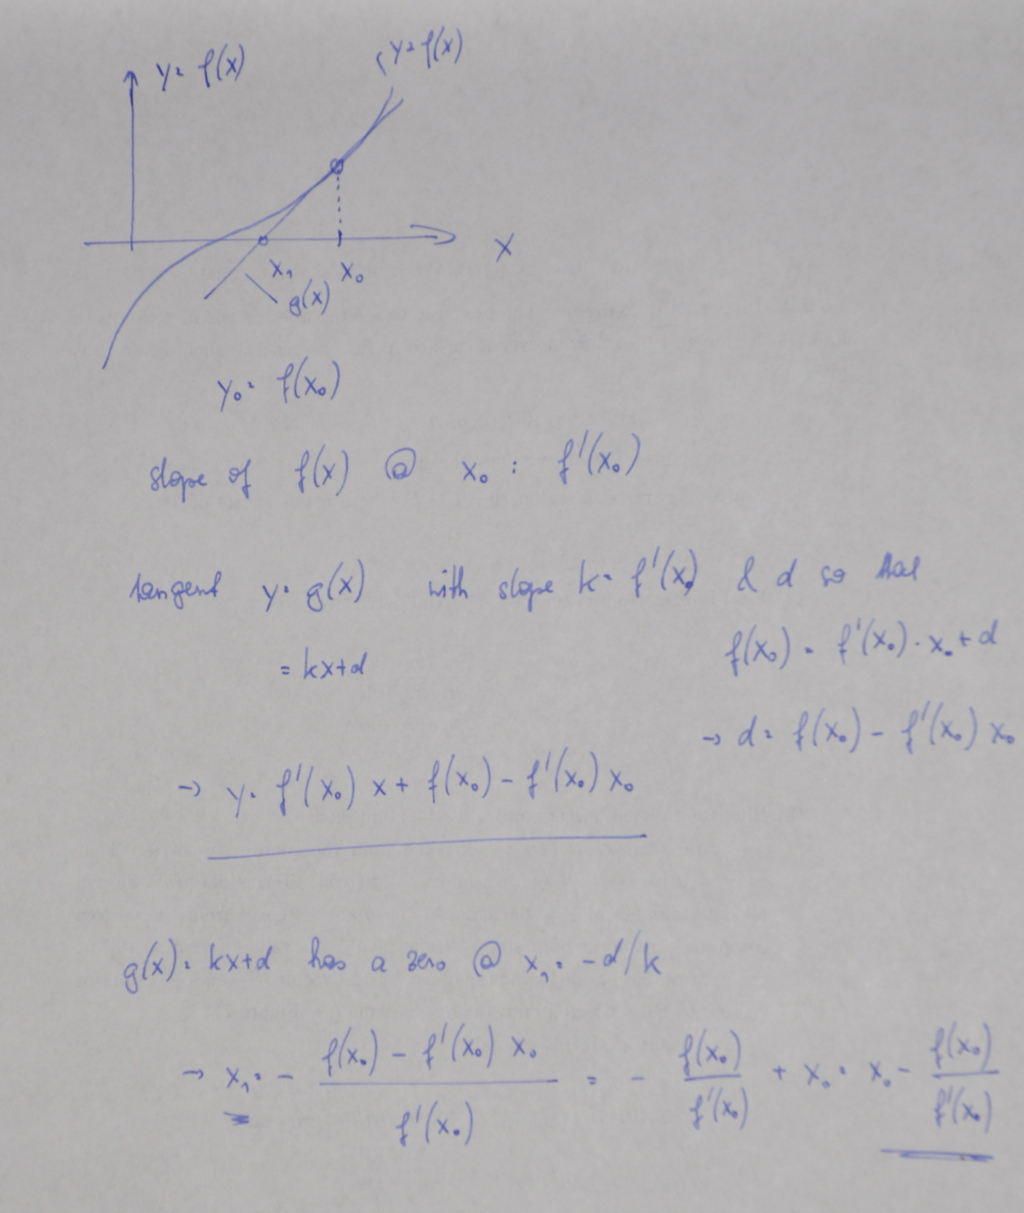
\includegraphics[scale=1.5]{images/DSC_0001_small.JPG}
\caption{Page1}
\end{figure}

e.g. \(f(x) = x^2-4\); then \(f'(x) = 2x\) and
\(x_{n+1} = x_n - (x^2-4)/(2x)\)

see
\href{file:///home/cnovak/src/julia/JuliaStuff/newton.jl}{newton.jl}:

\begin{verbatim}
function newton_solve(z0)
# solve x^2 - 4 = 0
    z = z0
    for n=1:20
        z = z - (z*2-4)/(2*z)
        println(n, " -> ", z)
    end
    return z
end

println(newton_solve(4))
\end{verbatim}

yields

\begin{verbatim}
1 -> 3.5
2 -> 3.0714285714285716
3 -> 2.722591362126246
4 -> 2.457185626921853
5 -> 2.271124947617549
6 -> 2.151745805619235
7 -> 2.0812236253398755
8 -> 2.0421967642419427
9 -> 2.021534326135688
10 -> 2.0108818599087837
11 -> 2.0054703734730377
12 -> 2.0027426475762127
13 -> 2.001373201741756
14 -> 2.000687071968178
15 -> 2.0003436539605324
16 -> 2.0001718564997053
17 -> 2.000085935632882
18 -> 2.000042969662595
19 -> 2.0000214852928857
20 -> 2.000010742761846
2.000010742761846
\end{verbatim}

%\DiaryEntry{Probability of the Union of Events}{2015-07-21}{Stochastic}


Based on
\href{https://terrytao.wordpress.com/2010/01/01/254a-notes-0-a-review-\%20\%5Bof-probability-theory/}{Exercise
15} in Terry Tao's blog.

Two events $E_1, E_2$ with probabilites $P(E_1) = P_1, P(E_2) = P_2$. Below we assume independent events; that is $P(E_1, E_2) = P(E_1) \times P(E_2)$; or, to be more exact $P(E_1=e_1 \cap E_2=e_2) = P(E_1=e_1) \times P(E_2=e_2)$.

\begin{figure}[hbt!]
\centering
\includegraphics[scale=0.5]{images/union_probability.png}
\caption{Page1}
\end{figure}

Similar (probability is proportional to the size of sets), there is the Sieve Formula for calculating the size of the union of sets:

\[ |A_1 \cup A_2 \cup \cdots A_n| = \sum_{j=1}^n (-1)^{j-i} \sum_{i_1, i_2, i_j} | A_{i_1} \cap A_{i_2} \cap \cdots A_{i_j}|\]

where $i_1, i_2, \ldots , i_j$ covers all j-element subsets of $[n]$.

For the case $n=2$, we therefore have

\[ |A_1 \cup A_2| = |A_1| + |A_2| - |A_1 \cap A_2| \]

for $n=3$, we have

\[ |A_1 \cup A_2 \cup A_3 | = |A_1| + |A_2| + |A_3| - |A_1 \cap A_2| - |A_1 \cap A_3| - |A_2 \cap A_3| + |A_1 \cap A_2 \cap A_3| \].

Compare this with the results in the handwritten notes above.

%\DiaryEntry{Gamma Function}{2015-07-27}{Maths}

\subsection{Partial Integration}

First thing is the derivation of the partial integration: We differentiate the product of two functions

\bee
\frac{d (u(x)v(x)}{dx} = u(x) \frac{d v(x)}{dx} + v(x) \frac{d u(x)}{dx}
\eee
%
integrate both sides

\bee
u(x)v(x) = \int u(x) \frac{d v(x)}{dx} dx + \int v(x) \frac{d u(x)}{dx} dx
\eee
%
and rearrange the result so that we obtain
%
\bee
\int u(x) \frac{d v(x)}{dx} dx = u(x)v(x) - \int v(x) \frac{d u(x)}{dx} dx
\eee
%
or - in a more sloppy notation - we have
%
\bee
\int u v' dx = uv - \int u' v dx
\eee

\subsection{Definition and Properties}

The Gamma function $\Gamma(x)$ is defined according to
%
\bee
\Gamma(x) = \int_0^\infty t^{x-1}e^{-t} dt
\eee

The following Figure shows a plot of the integrand for $x=1, x=2, x=3$, respectively. Note that with increasing $x$, the maximum moves to the right and the area under the curve increases.

\begin{figure}[hbt!]
\centering
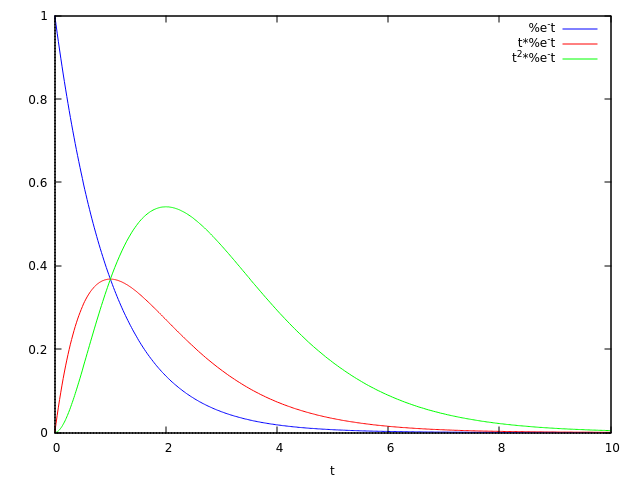
\includegraphics[scale=0.7]{images/gamma_integrand_plot.png}
\end{figure}

\pagebreak

Note, that the Gamma function is also defined for negative values of $x$; the following Figure shows plots of the integrand for $x=-1, x=-2, x=-3$, respectively. It diverges at $t=0$, and falls off for increasing $t$.

\begin{figure}[hbt!]
\centering
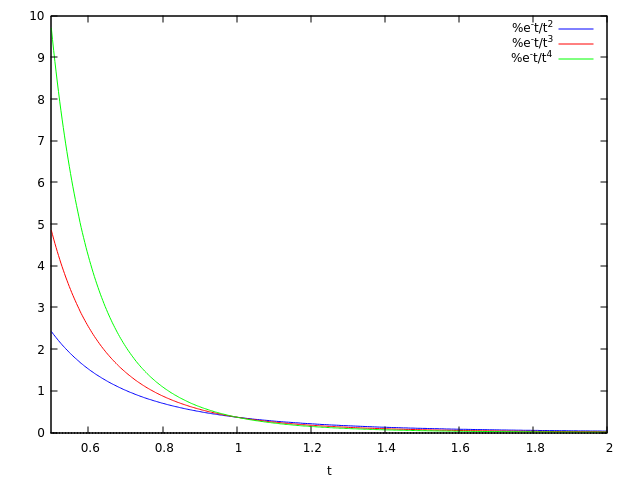
\includegraphics[scale=0.7]{images/gamma_integrand_neg_plot.png}
\end{figure}


The Gamma function fulfills the following recurrence relation
%
\bee
\Gamma(x+1) = x \Gamma(x)
\eee
%
which we can prove as follows
%
\bee
\Gamma(x+1) = \int_0^\infty t^{x}e^{-t} dt
\eee
by partial integration ($v'e^{-t} \rightarrow v = -e^{-t}, u=t^x \rightarrow u'=x t^{x-1}$) we obtain
%
\bee
\Gamma(x+1) = \left. -t^x e^{-t} \right|_0^\infty - \int_0^\infty x t^{x-1}(-1)e^{-t} dt = 0 + \int_0^\infty x t^{x-1}e^{-t} dt = x \int_0^\infty t^{x-1}e^{-t} dt
\eee
%
where in the last step we have used the fact that the integral is over $t$ and therefore $x$ can be taken out of the integral. Comparing with the definition, we see that
%
\bee
\Gamma(x+1) = x \Gamma(x) \qed
\eee
%
Next we calculate the value of $\Gamma(1)$ as
%
\bee
\Gamma(1) = \int_0^\infty t^{0}e^{-t} dt = \int_0^\infty e^{-t} dt = \left. e^{-t} \right|_0^\infty = 1
\eee
%
The function plot looks as follows (be careful; Julia uses a gamma function shifted by one):

\begin{figure}[hbt!]
\centering
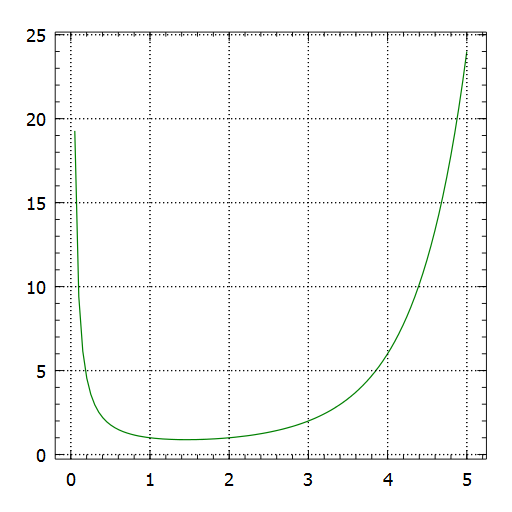
\includegraphics[scale=0.5]{images/gamma_plot.png}
\end{figure}

%\DiaryEntry{Digital Ocean Setup Notes}{2015-07-28}{General}


\subsection{Users}\label{users}

root / das übliche

cno / das übliche

\subsection{Package Installation}\label{package-installation}

\begin{verbatim}
apt-get install <package name>

apt-cache search <search name>
\end{verbatim}

\subsection{CLI Window Manager}\label{cli-window-manager}

\href{https://www.digitalocean.com/community/tutorials/how-to-use-dvtm-and-dtach-as-a-terminal-window-manager-on-an-ubuntu-vps}{Using
dvtm and dtach}

\paragraph{Using dvtm}\label{using-dvtm}

DVTM is a window manager for the console. It allows to manage several
windows (open, close, switch to\ldots{}).

\begin{verbatim}
C-g

    c ... create new window

    j/k ... cycle through open windows

    x ... destroy current window

    q ... destroy all windows and exit

    space ... change window tiling-mode

    m ... switch to full-screen window tiling mode
\end{verbatim}

\paragraph{Using detach}\label{using-detach}

Dtach is like screen for use together with DVTM.

Start / reattach to a session

\begin{verbatim}
dtach -A /tmp/dvtm -r winch dvtm
\end{verbatim}

\subsection{PostgreSQL}\label{postgresql}

Access to standard port 5432 is not possible from FRQ; use an iptable rule to forward connection from localhost:80 to localhost:5432 \href{see:\%20http://serverfault.com/questions/112795/how-can-i-run-a-server-on-linux-on-port-80-as-a-normal-user}{according to this link}.

\begin{itemize}

\item create iptables rule

\begin{verbatim}
iptables -t nat -A PREROUTING -p tcp --dport 80 -j REDIRECT --to-port 5432
\end{verbatim}

\item show rules - chain prerouting

\begin{verbatim}
iptables -t nat --line-numbers -n -L
\end{verbatim}

\item delete rule number N from iptables:

\begin{verbatim}
iptables -t nat -D PREROUTING N
\end{verbatim}


\end{itemize}

%%\section{Markov Inequality, 2015-08-16}
%\label{2015-08-16:entry}

\DiaryEntry{Markov and Chebyshev Inequality}{2015-08-16}{Stochastic}

holds for non-negative random variable $X$ and $a > 0$. Consider an indicator function $I(\cdot)$ which is one when the condition is true and zero otherwise. Now distinguish between the two cases $X \geq a$ and $X < a$. If $X \geq a$, then $I(X \geq a) = 1$; if $X < a$, then $I(X \geq a) = 0$. We can collect this in a single expression, namely
%
\begin{equation*}
a I(X \geq a) \leq X
\end{equation*}
%
Taking expectation on both sides yields
%
\begin{equation*}
a \mathrm{E}(I(X \geq a)) \leq \mathrm{E}(X)
\end{equation*}
%
and we observe that $a \mathrm{E}(I(X \geq a)) = P(X \geq a)$ and therefore we have
%
\begin{equation*}
a P(X \geq a) \leq \mathrm{E}(X) \rightarrow P(X \geq a) \leq \frac{\mathrm{E}(X)}{a}
\end{equation*}
%
which is the famous Markov inequality.


\subsection*{Example}

Example for the exponential distribution $f(x) = \lambda e^{- \lambda x}$ as follows:
%
\begin{equation*}
P(X \geq a) =  \int_a^\infty \lambda e^{- \lambda x} = e^{- \lambda a}
\end{equation*}
%
The expectation is $E(X) = 1/\lambda$ and therefore we have
%
\begin{equation*}
P(X \geq a) \leq \frac{1}{\lambda a}
\end{equation*}
%
In the plot below the green curve shows the true value of $P(X \geq a)$; the blue curve is the Markov approximation.

\begin{figure}[h]
\centering
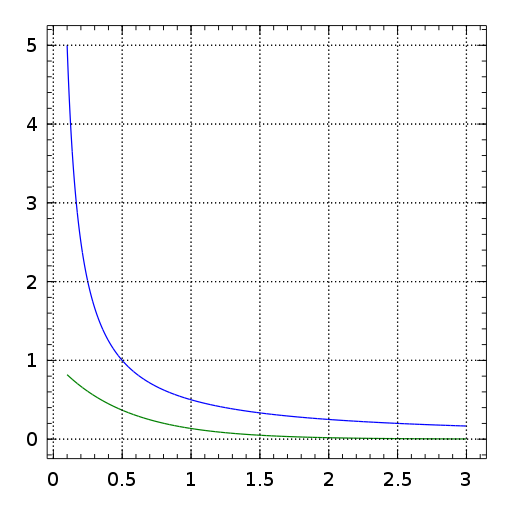
\includegraphics[scale=0.35]{images/exponential.png}
\caption{Exponential Distribution: Tail probabilities.}
\end{figure}

\subsection*{Chebyshev Inequality}

Whereas the Markov inequality holds only for positive RV's and requires only a known mean, the Chebyshev inequality holds for any RV with known (and existing) mean and variance.

We consider the absolute value of a RV $|X|$. Using the Markov inequality, we have
%
\begin{equation*}
  P(|Y| \geq a) \leq \frac{\mathrm{E}\{|Y|\}}{a}
\end{equation*}
%
We now consider a RV $Y = (X - \mu)^2$ and $a = (k \sigma)^2$ (where $\mu$ is the expectation of $X$ and $\sigma^2$ its variance) and we obtain
%
\begin{equation*}
  P(|X-\mu|^2 \geq (k \sigma)^2) \leq \frac{\mathrm{E}\{(X-\mu)^2\}}{(k \sigma)^2} = \frac{\sigma^2}{k^2 \sigma^2} = 1 / k^2
\end{equation*}
%
%
We therefore arrive at the Chebyshev inequality
%
\begin{equation*}
    P(|X-\mu|^2 \geq (k \sigma)^2) \leq 1 / k^2
\end{equation*}
%
or
%
\begin{equation*}
    P(|X-\mu| \geq k \sigma) \leq 1 / k^2
\end{equation*}


\subsubsection*{Example: Normal Distribution}

Normal distribution with zero mean $\mathcal{N}(0, \sigma^2)$. $P(X \leq x) = F(x) = \frac{1}{2} \left[ 1 + \erf \frac{x}{\sigma\sqrt{2}} \right]$ (see \href{https://en.wikipedia.org/wiki/Normal_distribution}{Wikipedia}). Then $P(|X| \geq a) = 2 F(-a)$ or $P(|X| \geq k\sigma) = 2 F(-k\sigma) = 1 + \erf \frac{-k}{\sqrt{2}}$, which ``interestingly'' does not depend on $\sigma$ but only on $k$.
%
The bound using Chebyshev's inequality states that $P(|X| \geq k \sigma) \leq 1/k^2$.

\subsubsection*{Example: Mean of RVs}

We have $N$ iid RVs with mean \(\mu_x\) and variance \(\sigma_x^2\) and calculate the mean
%
\begin{equation*}
M = \frac{1}{N} \sum_i x_i
\end{equation*}
%
which has mean \(E\{M\} = \frac{1}{N} N \mu_x = \mu_x\) and variance \(E\{(M-\mu_x)^2\} = \frac{\sigma_x^2}{N}\). Using Chebyshev's inequality, we have
%
\begin{equation*}
P \left(| X-\mu_x |^2 \geq k^2 \frac{\sigma_x^2}{N} \right) \leq \frac{1}{k^2}
\end{equation*}
%
Now we can set \(\alpha = k^2 \frac{\sigma_x^2}{N}\) (and therefore \(\frac{1}{k^2} = \frac{\sigma_x^2}{\alpha N}\)) and finally obtain
%
\begin{equation*}
P \left(| X-\mu_x |^2 \geq \alpha \right) \leq \frac{\sigma_x^2}{\alpha N}
\end{equation*}
%
By considering ``enough'' RVs in the mean calculation, we can make the deviation of \(M\) arbitrarily small around the mean \(\mu_x\).

%\DiaryEntry{Normal Distribution}{2015-08-17}{Stochastic}

A short summary of things I keep forgetting, mostly based on \href{https://en.wikipedia.org/wiki/Normal_distribution}{Wikipedia}.
%
Normal distribution with mean $\mu$ and variance $\sigma^2$: $\Nc(\mu, \sigma^2)$.

\subsection{PDF}\label{pdf}

The pdf has the following form:

\[f(x) = \frac{1}{\sqrt{2\pi\sigma^2}} e^{ - \frac{(x-\mu)^2}{2\sigma^2} }\]

\subsection{CDF}\label{cdf}

The CDF $F(x)$ gives the probability $P(X < x ) = F(x)$. There is no closed form available; use the error function instead:

\[\text{erf}(x) = \frac{1}{\pi} \int_{-x}^x e^{-t^2/2}\]
%
The error function gives the probability of a normal RV with zero mean variance $1/2$ falling into the range $[-x;x]$.
%
With this we obtain for a RV with normal distribution $\mathcal{N }(\mu, \sigma^2)$:

\[F(x) = P(X < x)  = \frac{1}{2} \left[ 1 + \text{erf} \left( \frac{x-\mu}{\sqrt{2\sigma^2}} \right) \right] \]
%
In Julia we can do this as follows:

\begin{verbatim}
# generate N random normal RVs
N = 1000000

# with variance s2
s2 = 1.5

x = sqrt(s2)*randn(N)

# find the prob of X < xlim
xlim = 1.2

# empirically
println(count(x->x<xlim, x)/N)

# with the error function
trueval = 0.5*(1+erf(xlim/(sqrt(2*s2))))
\end{verbatim}
%
By the way, note the elegant way of counting the elements of the vector \texttt{x} which are less than \texttt{xlim}. Using these definitions, we can also calculate other probabilities; e.g.
%
\[P(a < X < b) = F(b) - F(a); \qquad b > a\]
%
Empirically measured in Julia via \texttt{println(count(x-\textgreater{}x\textgreater{}a\ \&\&\ x\textless{}b,\ x)/N)}. Another probability is
%
\[P(X > a) = 1 - F(a),\]
%
empirically measured in Julia via \texttt{println(count(x-\textgreater{}x\textgreater{}a,\ x)/N)}.

%\DiaryEntry{Geometric Distribution}{2015-08-18}{Stochastic}

Two definitions, but the same principle: Number of Bernoulli trials, before the trial succeeds.

The success probability of the Bernoulli trial is denoted by $p$; the random variable $X$ denotes the number of trials $k$ before a trial succeeds and therefore has a pmf as follows:

\[ P(X=k) = (1-p)^k p\]

\subsection{Expectation}

The expectation $\mathcal{E}(X)$ is calculated as follows

\[\mathcal{E}(X) = \sum_{k=0}^\infty k \times P(X=k) = \sum_{k=0}^\infty k (1-p)^k p \]

We can rewrite this as

\[\mathcal{E}(X) = p(1-p) \sum_{k=0}^\infty k (1-p)^{k-1} \]

and realize that the summand can be written as differential

\[k(1-p)^{k-1} = - \frac{d}{dp} (1-p)^k\]

Exchanging summation with differentiation, we obtain

\[\mathcal{E}(X) = -p(1-p) \frac{d}{dp} \sum_{k=0}^\infty (1-p)^k \]

The sum is the geometric series
$\sum_{k=0}^\infty q^k = \frac{1}{1-q}$ with $q=1-p$, and we therefore have

\[\mathcal{E}(X) = -p(1-p) \frac{d}{dp} \frac{1}{p} = p(1-p)\frac{1}{p^2} = \frac{1-p}{p}\]

For small $p$, the expectation is large; i.e.~it takes a long time, before the trial succeeds. If $p=1/2$, $\mathcal{E}(X)=1$; i.e.~success is reached after 1 trial. Finally for $p=1, \mathcal{E}(X)=0$.

\subsection{Example}

Consider a dice with probability $p=1/6$ that one side comes up (e.g.~6). Then the RV $X$ denotes the number of trials, before this side comes up. The expectation is $\mathcal{E}(X) = \frac{1-p}{p} = \frac{5/6}{1/6} = 5$; i.e.~it takes 5 rolls, \textbf{before} this side comes up. In other words, on average, the 6-th roll shows the side.

\subsection{Sequences}

Consider a sequence of such trials: After a successful trial, the process is started again ad infinitum. The average time between successes (and therefore process restarts) is $\mathcal{E}(X)$. Therefore a length-N sequence contains $1/\mathcal{E}(X)$ successful trials.


\DiaryEntry{Interesting Integrals, 1}{2015-09-12}{Integrals}

\subsection{Simplification by Integrand Division}

The first integrals are taken from
\href{http://folk.ntnu.no/oistes/Diverse/Integral\%20Kokeboken.pdf}{here}.

\bee
\int \frac{x}{ax+b} dx = \int \frac{1}{b} - \frac{a}{b} \frac{1}{a+bx} dx = \frac{x}{b} - \frac{a}{b^2} \ln(a+bx)
\eee

where we have used "normal" division to go from the first expression to the second. The second integral is solved by substitution $u=a+bx, du/dx=a \rightarrow dx = du/b$.

\bee
\int \frac{1}{a+bx} dx = \int \frac{1}{u} \frac{du}{b} = \frac{1}{b} \ln u = \frac{1}{b} \ln a+bx
\eee

The same trick of dividing the integrand to simplify expressions can also be used here

\bee
\int \frac{x^2}{x+1} dx = \int x-1 + \frac{1}{x+1} dx = \frac{x^2}{2} - x + \ln(x+1)
\eee

which can be generalized to

\bee
\int \frac{x^2}{a+bx} dx = \int \frac{1}{b}x - \frac{a}{b^2} + \frac{a^2}{b^2} \frac{1}{a+bx} dx = \frac{x^2}{2b} - \frac{a}{b^2}x + \frac{a^2}{b^2} \ln(a+bx)
\eee

\subsection{Substitution Tricks}

This integral is from a paper by Victor H. Moll \href{http://arxiv.org/abs/0707.2122v1}{THE INTEGRALS IN GRADSHTEYN AND RYZHIK. PART 7: ELEMENTARY EXAMPLES}, although there is a small error in the paper (forgotten minus).

\bee
\int (1-\sqrt{x})^{p-1}dx
\eee

We use the "obvious" substitution $u=1-\sqrt{x}$ and obtain $du/dx = -\frac{1}{2}x^{-1/2} = - \frac{1}{2\sqrt{x}}$ and therefore $dx = -2\sqrt{x}du$. At first sight, we cannot use this substitution, as it still includes $x$. However, we can use the substitution in the form $\sqrt{x} = 1-u$ and obtain $dx = -2(1-u)du = 2(u-1)du$ and therefore obtain the new integral

\bee
\int u^{p-1} 2(u-1)du = 2 \int u^p - u^{p-1} du = 2 \left( \frac{u^{p+1}}{p+1} - \frac{u^p}{p} \right) = 2 \left( \frac{(1-\sqrt{x})^{p+1}}{p+1} - \frac{(1-\sqrt{x})^p}{p} \right)
\eee


This trick can be widely used; for example in

\bee
\int \frac{dx}{a+be^{mx}}
\eee

Setting $u=a+be^{mx}$ we have $\frac{du}{dx}=mbe^{mx}=m(u-a)$, where we have reused the substitution. Then $\frac{du}{dx}$ becomes

\bee
\frac{du}{dx} = m b e^{mx} = m(u-a) \rightarrow dx = \frac{du}{m(u-a)}
\eee

And the integral becomes

\bee
\int \frac{dx}{a+be^{mx}} = \int \frac{1}{u} \frac{du}{m(u-a)} = \frac{1}{m} \int \frac{du}{u(u-a)}
\eee

which can be solved via partial fraction decomposition.


\DiaryEntry{Interesting Integrals, 2}{2015-09-17}{Integrals}


\subsubsection{Integrals based on arctan}

Consider the integral (based on differentiation of arctan; see blog entry from 2015-08-25).


\[\int \frac{dx}{1+x^2} = \arctan x\]

From this we get for the definite integrals

\[ \int_0^1 \frac{dx}{1+x^2} = \arctan 1 = \frac{\pi}{4}\]

and

\[ \int_1^\infty \frac{dx}{1+x^2} = \arctan \infty - \arctan 1 = \frac{\pi}{4}\]

Funny that these integrals yield the same value.

The case of $\int\frac{x}{1+x^2}$ is simpler; set $u=1+x^2 \rightarrow dx = \frac{du}{2x}$, and we get

\[\int\frac{x}{1+x^2} = \frac{1}{2} \int \frac{du}{u} = \frac{1}{2} \ln(1+x^2)\]

A slightly more tricky integral is

\[\int \frac{1}{a+x^2} dx = \frac{1}{a} \int \frac{dx}{x^2/a+1}\]

With $u^2 = x^2/a$, we get $u = x / \sqrt{a} \rightarrow \frac{du}{dx} = 1 / \sqrt{a}$ and $dx = \sqrt{a} du$. Substitution back into the integral yields

\[ \frac{1}{a} \int \frac{dx}{x^2/a+1} = \frac{1}{a} \int \frac{\sqrt{a} du}{1+u^2} = \frac{\arctan (x/\sqrt{a})}{\sqrt{a}}\]

This is nice and useful and allows integration of

\[\int \frac{dx}{x^2+x+1} = \int \frac{dx}{(x+1/2)^2 + 3/4} \]

by completing the square. Setting $u = x+1/2$, we obtain $\frac{du}{dx} = 1$, and therefore

\[\int \frac{dx}{(x+1/2)^2 + 3/4} = \int \frac{du}{u^2 + 3/4} = \frac{\arctan (u/\sqrt{3/4})}{\sqrt{3/4}} = \frac{\arctan \left( \frac{x+1/2}{\sqrt{3/4}} \right)}{\sqrt{3/4}}\]

which can be further simplified to

\[ \int \frac{dx}{x^2+x+1} = \frac{2 \arctan \left( \frac{2x+1}{\sqrt{3}} \right)}{\sqrt{3}} \]

The final generalization is the integral $\int\frac{dx}{x^2+bx+c}$ which can be calculated by completing the square according to
$x^2+bx+c = (x+b/2)^2 + c - b^2/4$. With $u=x+b/2$ we
obtain $du=dx$, and finally

\[ \int\frac{dx}{x^2+bx+c} = \int \frac{du}{u^2 + c - b^2/4} = \frac{\arctan \frac{x+b/2}{\sqrt{c-\frac{b^2}{4}}}}{\sqrt{c-\frac{b^2}{4}}}\]

\subsubsection{Integrals based on arcsin}

From the blog entry on 2015-08-25 we have

\[\int \frac{dx}{\sqrt{1-x^2}} = \arcsin x\]

Generalizing, we obtain

\[\int \frac{dx}{\sqrt{a^2-x^2}} = \int \frac{dx}{a\sqrt{1-x^2/a^2}} \]

Substituting $u=x/a$, we get $dx = a du$ and finally

\[\int \frac{dx}{a\sqrt{1-x^2/a^2}} = \int \frac{du}{\sqrt{1-u^2}} = \arcsin \frac{x}{a}\]

Now consider the integral

\[ \int \frac{dx}{\sqrt{1-x-x^2}} \]

We can manipulate the expression
$1-x-x^2$ as follows

\[1-x-x^2= 1-(x^2+x) = 1-\left(x+\frac{1}{2}\right)^2+\frac{1}{4} = \frac{5}{4} - \left( x+\frac{1}{2} \right)^2\]

Setting $u=x+\frac{1}{2}$, we obtain for the integral

\[ \int \frac{dx}{\sqrt{1-x-x^2}} = \int \frac{du}{\sqrt{\frac{5}{4} - u^2}} = \arcsin \frac{u}{\sqrt{5/4}} = \arcsin \frac{2x+1}{\sqrt{5}}\]

\subsubsection{Trick: Completing the Square}

Most integrals were solved by a completing the square trick: Consider $x^2+x+1$. We can use an expression of the form $(x+1/2)^2 = x^2 + x + 1/4$ where the coefficients for $x^2$ and
$x$ are correct; only the coefficient for $x^0$ is wrong. We can correct this coefficient by adding a constant to the expression so that it becomes correct:

\[ x^2+x+1 = \left(x+\frac{1}{2}\right)^2 + \frac{3}{4} \]

Now we can e.g.~substitute $u=x+\frac{1}{2}$ which has the
additional advantage that $\frac{du}{dx} = 1$.


\DiaryEntry{Interesting Sums, 1}{2015-09-19}{Sums}


\subsubsection{Geometric Series}

We want to calculate the sum

\[ S_N = \sum_{k=1}^N a s^k \]

Consider the following expression

\[ S_N + a s^{N+1} = a s^0 + \sum_{k=0}^N a s^{k+1} = a s^0 + s \sum_{k=0}^N a s^k = a s^0 + s S_N \]

From this we obtain \textbackslash{}( S\_N (1 - s) = a - a s\^{}\{N+1\}
\textbackslash{}) and can finally express the sum as

\[ S_N = a \frac{1 - s^{N+1} }{1 - s} \]

If $|s| < 1$, then the sum converges for $N \rightarrow \infty$ to $S\_\infty=\frac{a}{1-s}$.

\subsubsection{Calculating $\sum k a^k$}

Next we want to tackle the sum

\[ S_N = \sum_{k=1}^N k a^k = a + 2a^2 + 3a^3 + \cdots + Na^N\]

We write down $a S\_N$ as follows

\[ a S_N = \sum_{k=1}^N k a^{k+1} = \sum_{k=1}^{N+1} (k-1) a^{k} = \sum_{k=1}^{N} (k-1) a^{k} + N a^{N+1} = a^2 + 2 a^3 + 3 a^4 + \cdots + N a^{N+1}\]

From this we see that the difference $S\_N - a S\_N$ has an easy form:

\[ S_N - a S_N = \sum_{k=1}^N k a^k - \left( \sum_{k=1}^{N} (k-1) a^{k} + N a^{N+1} \right) = \sum_{k=1}^N a^k - N a^{N+1} \]

The sum is the one we calculated above, so we have

\[ S_N - a S_N = \frac{a - a^{N+1} }{1 - a} - N a^{N+1} = \frac{a - a^{N+1} - N a^{N+1}(1-a)}{1-a} = \frac{a - a^{N+1} - N a^{N+1} + N a^{N+2}}{1-a} \]

Solving the equation for $S_N$, we get

\[S_N = \frac{a - a^{N+1}(N+1) + N a^{N+2}}{(1-a)^2} \]

If $|a| < 1$, then the sum converges for $N \rightarrow \infty$ to $S\_\infty = \frac{a}{(1-a)^2}$.

There is a different way (see blog entry on 2015-09-07 "Generating Functions 03") which may be easier: Start with

\[ \sum_{k=1}^N a^k = \frac{1 - a^{N+1} }{1 - a} \]

Taking the derivative on both sides and multiplying with $a$, we obtain

\[ \sum_{k=1}^N k a^k = a \frac{d}{da} \frac{1 - a^{N+1} }{1 - a} \]

We can check all 3 results with Python / Julia as follows. Start with Julia and calculate the ``ground truth''

\begin{verbatim}
n = 1:10
a=0.4

sum(n.*a.^n)
1.110295552
\end{verbatim}

In Python we can check with Sympy

\begin{verbatim}
import sympy as sym

x, n, a = sym.symbols("x n a")
f = (x**(n+1)-1)/(x-1)
g = sym.diff(f, x)
res = g*x
sym.pprint(res.subs(x,0.4).subs(n,10))
1.110295552
\end{verbatim}

which is the same as the expression calculated above. Finally

\begin{verbatim}
print( (a - (N+1)*a**(N+1) + N*a**(N+2))/(1-a)**2)
1.110295552
\end{verbatim}

which shows the correctness of the approach taken above.


\DiaryEntry{Interesting SSums, 2}{2015-09-19}{Sums}

\subsection{$\sum \frac{1}{k^2} = \frac{\pi^2}{6}$


We consider the infinite sum $\sum_{k=1}^\infty \frac{1}{k^2}$;
the derivation is based on \href{http://math.stackexchange.com/questions/8337/different-methods-to-compute-sum-limits-k-1-infty-frac1k2}{this discussion}.

In the interval $0 < x < \pi/2$, we have $0 < \sin x < x < \tan x$ and therefore

\[\frac{1}{\tan^2 x} < \frac{1}{x^2} < \frac{1}{\sin^2 x} \]

Using the fact that $1/\tan^2 x = 1/\sin^2 x -1$, we obtain

\[\frac{1}{\sin^2 x} - 1 < \frac{1}{x^2} < \frac{1}{\sin^2 x} \]

To get a sum, we split the interval $(0, \pi/2)$ (the one the inequality above holds) into $2^n$ equal parts, and sum the
inequality over the gridpoints

\[ \sum_{k=1}^{2^n-1} \left( \frac{1}{\sin^2 x_k} - 1 \right) < \sum_{k=1}^{2^n-1} \frac{1}{x_k^2} < \sum_{k=1}^{2^n-1} \frac{1}{\sin^2 x_k} \]

where the gridpoints are defined as $x_k = \frac{\pi}{2} \frac{k}{2^n}$. Denoting the right sum as $S_n$, we can write

\[ S_n - (2^n-1)  < \sum_{k=1}^{2^n-1} \left( \frac{2 \cdot 2^n}{\pi}\right)^2 \frac{1}{k^2} < S_n \]

This is already quite close to the equality we want to show. Next steps ae (i) calculate $S_n$ and (ii) show that the mid-expression is ``sandwiched'' between the left and right expression.

In order to evaluate $S_n$, start with the observation that $\sin (\pi/2 - x) = \cos x$ and therefore

\[ \frac{1}{\sin^2 x} + \frac{1}{\sin^2 (\pi/2 - x)} = \frac{\cos^2 x + \sin^2 x}{\cos^2 x \sin^2 x} = \frac{4}{\sin^2 2x}\]

That is, instead of calculating the sum $S_n$ on $2^n$ points, we can consider four times the sum $S_{n-1}$ (consisting
of only $2^{n-1}$ points) and consider the contribution of the interval midpoint $\pi/4$ which equals 2 in order to arrive at the relation

\[S_n = 4 S_{n-1} + 2\]

We use generating functions in order to find a closed-form expression for $S_n$; this is done in the appendix. We arrive at the following expression:

\[S_n = \frac{2}{3}(4^n-1)\]

And now we have

\[ \frac{2}{3}(4^n-1) - (2^n-1)  < \sum_{k=1}^{2^n-1} \left( \frac{2 \cdot 2^n}{\pi}\right)^2 \frac{1}{k^2} < \frac{2}{3}(4^n-1) \]

which we can rewrite as

\[ \frac{2}{3}(4^n-1) - (2^n-1)  < \frac{4^{n+1}}{\pi^2} \sum_{k=1}^{2^n-1} \frac{1}{k^2} < \frac{2}{3}(4^n-1) \]

If we divide by the factor in front of the sum, we obtain

\[ \frac{\pi^2}{4^{n+1}} \frac{2}{3}(4^n-1) - \frac{\pi^2}{4^{n+1}} (2^n-1)  < \sum_{k=1}^{2^n-1} \frac{1}{k^2} < \frac{\pi^2}{4^{n+1}} \frac{2}{3}(4^n-1) \]

and this can be further simplified to

\[ \frac{2}{3} \pi^2 \frac{4^n-1}{4^{n+1}} - \frac{\pi^2}{4^{n+1}} (2^n-1) < \sum_{k=1}^{2^n-1} \frac{1}{k^2} < \frac{2}{3} \pi^2 \frac{4^n-1}{4^{n+1}} \]

In the event that $n\rightarrow \infty$, the second term on the left goes to zero and the remaining terms on the left and right side are equal. There the sum in the middle is squeezed in by the RHS and LHS and converges to

\[\sum_{k=1}^\infty \frac{1}{k^2} = \frac{2}{3} \pi^2 \frac{1}{4} = \frac{\pi^2}{6} \]

\subsection{Appendix: Closed-form expression of $S_n$}

We seek a closed-form expression for

\[S_n = 4 S_{n-1} + 2, \quad S_1 = 2\]

According to the procedure described in the generating function series,
we have to convert this as follows:

\[S_{n+1} = 4 S_{n} + 2, \quad S_1 = 2\]

i.e.~there shall be no $n-1,n-2,\ldots$. The initial conditions are also tricky in case of a difference equation of first order (time delay is 1), there must be an initial condition for $S_0$,
\textbf{not} for $S_1$.

But this is easy; we can use the recurrence equation to determine
$S_0$:

\[ S_1 = 4 S_0 + 2 \rightarrow S_0 = 1/4 \times (S_1-2) = 0 \]

Now things become easy: Transforming the recurrence equation yields

\[\frac{A(z)-S_0}{z} = 4A(z) + \frac{2}{1-z} \rightarrow \frac{A(z)}{z} = 4A(z) + \frac{2}{1-z} \]

where $A(z)$ is the generating function of $S_n$. From this we obtain

\[ A(z) =  \frac{2z}{(1-z)(1-4z)} = \frac{2}{3} \left( \frac{1}{1-4z} - \frac{1}{1-z} \right)\]

(the partial fraction expansion was done via Wolfram Alpha) and conclude
that

\[ S_n = \frac{2}{3} \left(4^n - 1\right) \]


\DiaryEntry{Triangular Numbers}{2015-10-08}{Maths}

\subsection{Basics}

Based upon \href{https://en.wikipedia.org/wiki/Triangular_number}{Wikipedia}.

These are the number of nodes that form an equilateral triangle, as
shown below.

\todo{FIGURE}
\begin{figure}
\centering
%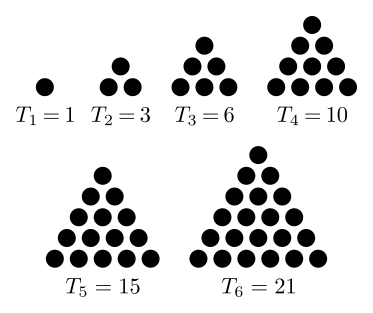
\includegraphics{/images/triangular_numbers.svg}
\end{figure}

The $n$-th triangle number is the number of nodes composing a triangle with n nodes on a side, and is equal to the sum of the $n$ natural numbers from
$1$ to $n$. That is,

\[ T_n = \sum_{i=0}^n n = \frac{n(n+1)}{2} \]

We had this sum before but there are two other alternatives; one based on an geometric argument; the other uses generating functions.

\subsubsection{Geometric Argument}

Consider the Figure below; there are $5 \times 5 = 25$ nodes. The green and black ones are each $T_4$, and there are
$5$ red ones. Therefore, the total number of nodes can also be expressed as $2 \times T_4 + 5$.

\todo{FIGURE}
\begin{figure}
\centering
%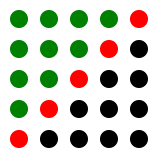
\includegraphics{/images/triangular_numbers_2.svg}
\end{figure}

Generalizing to arbitrary $n$, we have

\[n^2 = 2 \times T_{n-1} + n \rightarrow T_{n-1} = \frac{n^2 - n}{2} = \frac{n(n-1)}{2} \]

or

\[T_{n} = \frac{n(n+1)}{2}\]

This is a classic of counting the same arrangements in a different
(preferably simpler) way.

\subsubsection{Generating Functions}

Converting the sum $T_n \sum_{i=0}^n i$ into a recurrence relation, we obtain $T_n = T_{n-1} + n$; or equivalently

\[ T_{n+1} = T_n + (n+1); \qquad T_0 = 0\]

We can convert this into an expression for the generating function
$A(z)$ of $T_n$; namely

\[ \frac{A(z)-T_0}{z} = A(z) + \sum_{n \geq 0}n z^n + \sum_{n \geq 0} z^n \]

For the expression $\sum_{n \geq 0}n z^n$ we do the following: Consider the all-one series which generating function is $B(z) = \sum_{n \geq 0} 1 z^n = \frac{1}{1-z}$. We seek $n z^n$; this corresponds to $z B(z) = \frac{z}{(1-z)^2}$.

We therefore have

\[ \frac{A(z)-T_0}{z} = A(z) + \frac{z}{(1-z)^2} + \frac{1}{1-z} \rightarrow A(z) = \frac{z}{(1-z)^3}\]

A series expansion yields

\begin{verbatim}
      2     3      4      5      6      7      8      9
x + 3x  + 6x  + 10x  + 15x  + 21x  + 28x  + 36x  + 45x  + ...
\end{verbatim}

Another way would be to consider the sequence $1,2,3,4,\ldots$ with the generating function $A(z) = \sum_{n \geq 0} n z^n = \frac{z}{(1-z)^2}$. We want to obtain the sequence of the partial sums; the corresponding generating function is $\frac{A(z)}{1-z} = \frac{z}{(1-z)^3}$.

\subsubsection{Other Characteristics}

From the definition of the $T_n$, we have the following property:

\[ T_n + T_{n-1} = \frac{n(n+1)}{2} + \frac{n(n-1)}{2}  = n^2\]

and

\[ T_{n} - T_{n-1} = \frac{n(n+1)}{2} - \frac{n(n-1)}{2}  = n \]

Therefore, we have

\[ T_n + T_{n-1} = (T_{n} - T_{n-1})^2 \]

\subsection{Number of Line Segments}

Related to the triangular numbers are the numbers $L_n$ of direct connections between the objects; for example see the Figure below. For $n=4$ (red lines), we have $L_4 = 18$. Every node contributes
$3$ connections; therefore we have $L_n = 3 T_{n-1}$.


\todo{FIGURE}
\begin{figure}
\centering
%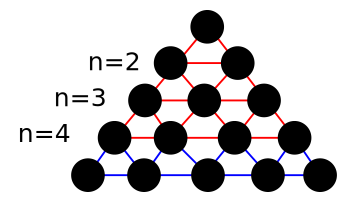
\includegraphics{/images/triangular_numbers_3.svg}
\end{figure}

A different argument leads to a recurrence relation for the $L_n$: If we have connections up to level $n$ ($n=4$) in the example above), then the next level adds another $3 \times n$ connections and we therefore have

\[ L_{n+1} = L_n + 3n\]

I.e. $L_5 = L_4 + 3 \times 4 = 18 + 12 = 30$.

\subsubsection{Generating Functions}

Just for the fun of it; we have

\[ \frac{A(z)}{z} = A(z) + 3 \sum_{n \geq 0} n z^n = A(z) + \frac{3z}{(1-z)^2} \rightarrow A(z) = \frac{3z^2}{(1-z)^3}\]

A series expansion yields

\begin{verbatim}
  2     3      4      5      6      7      8       9
3x  + 9x  + 18x  + 30x  + 45x  + 63x  + 84x  + 108x + ...
\end{verbatim}


\DiaryEntry{2D Integral Substitution}{2015-10-27}{Integrals}

We want to solve a 2D-integral

\[ I = \int_x \int_y f(x,y) dy dx \]

and want to perform a substitution: $x = x(u, v); y = y(u; v)$. The integrand then becomes $f(u,v)$. In addition we need to transform the "$dx dy$-square" into its equivalent "$du dv$-square". This is
achieved by the Jacobian matrix which is defined as:

\[ J(u,v) = \left( \begin{array}{cc}
\frac{\partial x(u,v)}{\partial u} & \frac{\partial x(u,v)}{\partial v}  \\
\frac{\partial y(u,v)}{\partial u} & \frac{\partial y(u,v)}{\partial v} 
\end{array} \right) \]

Then the integral can be rewritten as

\[ I = \int_x \int_y f(x,y) dy dx = \int_u \int_v f(u,v) |J(u,v)| dv du \]

with $|J(u,v)|$ denoting the determinant of the Jacobian Matrix.

\subsubsection{Simple Example}

As a toy example, consider the integral which can be solved by
elementary means

\[ I = \int_{x=0}^1 \int_{y=0}^1 x y^2 dy dx = \frac{1}{6}\]

Making the substitution $u=x/2, v=3y$ leads to $x=2u, y=v/3$ and to the following Jacobian Matrix:

\[J(u,v) = \left( \begin{array}{cc} 2 & 0 \\ 0 & \frac{1}{3} \end{array} \right) \]

With the determinant being
$|J(u,v)| = \frac{2}{3}$, we arrive at (note the changed integration intervals!):

\[I = \int_{u=0}^{\frac{1}{2}} \int_{v=0}^3 2u \frac{v^2}{9} \frac{2}{3} dv du = \frac{1}{6}\]

\subsubsection{Solving the Integrals with SymPy}

... works as follows:

\begin{verbatim}
import sympy as sym
x, y = sym.symbols("x y")

res = sym.integrate(x*y**2, (x,0,1), (y,0,1))
sym.pprint(res)

res_subs = sym.integrate(2/3*2*x*y**2/9, (x,0,1/2), (y,0,3))
sym.pprint(res)
\end{verbatim}

\subsubsection{Polar Coordinates}

Consider the substitution from rectangular coordinates to polar
coordinates with the transformation rules $x = r \cos \phi; y = r \sin \phi $. The Jacobian therefore becomes

\[J(r, \phi) = \left( \begin{array}{cc} \frac{\partial x}{\partial r} & \frac{\partial x}{\partial \phi} \\ \frac{\partial y}{\partial r} & \frac{\partial y}{\partial \phi} \end{array} \right)
 = \left( \begin{array}{cc} \cos \phi & -r \sin \phi \\ \sin \phi & r \cos \phi \end{array} \right) \]

The determinant is $|J(r, \phi)| = r \cos^2 \phi + r \sin^2 \phi = r$ and therefore we have for the integral

\[ I = \int_x \int_y f(x,y) dy dx = \int_r \int_\phi f(r \cos\phi, r \sin\phi) r dr d\phi \]


%\DiaryEntry{Topological Spaces}{2016-02-22}{Topology}

A topological space is a set, \(\mathcal{X}\), together with a
collection, \(\mathcal{T}\), of subsets of \(\mathcal{X}\). These
subsets are called ``open'' sets and satisfy the following rules:

\begin{itemize}
\item
  The set \(\mathcal{X}\) is ``open''
\item
  The empty set \(\mathcal{O}\) is open
\item
  Arbitrary unions of sets are ``open''
\item
  Finite intersections of ``open'' sets are ``open''
\end{itemize}

This collection \(\mathcal{T}\) is called the topology on
\(\mathcal{X}\). Note that here, the term ``open'' is a definition - any
set can be defined to be open. The 4 conditions are modeled similar to
the definitions of open sets of the real line \(\mathcal{R}\); the idea
is that the conditions ensure that open sets in a topological space
behave similar to open sets in \(\mathcal{T}\).

Therefore, the real line with the ``standard'' definition of openness is
a topological space.

\subsubsection{Example (indiscrete topology)}

We have the set \(\mathcal{B} = \{0,1\}\) and we can define a
topological space as follows: We define the empty set \(\mathcal{O}\)
and the set \(\mathcal{B}\) as open. This satisfies the first two axioms
from above. Because \(\{0,1\} \cup \mathcal{O} = \{0,1\}\) we have
satisifed the third axiom, and since
\(\{0,1\} \cap \mathcal{O} = \mathcal{O}\) which is open again, we have
also satisfied the fourth axiom. This topology is called an
\emph{indiscrete} topolgy.

\subsubsection{Example (discrete topology)}

However, we can also define a different topological space by defining
the sets \(\mathcal{O}, \{0\}, \{1\}, \{0,1\}\) as open. The empty set
and whole set are included, so axioms 1 and 2 are satisfied. Unions and
intersections always yield a set defined to be open; therefore, axioms 3
and 4 are also satisfied. This topology is called a \emph{discrete}
topolgy.

A subset \(\mathcal{X}\) is closed, when the complement
\(\mathcal{T} - \mathcal{X}\) is open.

In the indiscrete topology example above, both \(\mathcal{O}\) and
\(\{0,1\}\) are closed - that is, sets can be open and closed at the
same time! Since neither \(\{0\}\) and \(\{1\}\) are defined as open,
they are also not closed - sets can also be neither closed nor open at
the same time!

\subsection{Definition of Continuity}

A function (map) \(f: \mathcal{S} \rightarrow \mathcal{T}\) between two
topological spaces is continuous, if the preimage
\(f^{-1}(\mathcal{Q})\) of every open set
\(\mathcal{Q} \in \mathcal{T}\) is an open set in \(\mathcal{S}\).

This generalizes the definition of continuity for functions from
\(\mathcal{R}\) to \(\mathcal{R}\).

\subsubsection{Example}

Considering the example with the discrete topology from above. Define
the function \(f\) as \(f(0)=-1\) and \(f(1)=1\). Let \(\mathcal{U}\) be
any open set in \(\mathcal{R}\). The preimage of \(\mathcal{U}\) is then
given as

\[
f^{-1}(\mathcal{U}) = \begin{cases}
{0} & \mbox{if }  -1 \in \mathcal{U} \mbox{ and } 1 \notin \mathcal{U} \\
{1} & \mbox{if }  -1 \notin \mathcal{U} \mbox{ and } 1 \in \mathcal{U} \\
{0,1} & \mbox{if }  -1 \in \mathcal{U} \mbox{ and } 1 \in \mathcal{U} \\
\mathcal{O} & \mbox{if }  -1 \notin \mathcal{U} \mbox{ and } 1 \notin \mathcal{U} \\
\end{cases}
\]

In all cases, the preimage of \(\mathcal{U}\) is open, since every
subset of \(\mathcal{B}\) is open in the discrete topology. Therefore,
the function \(f\) is continuous.

%\DiaryEntry{Holomorphic FUnctions}{2016-02-24}{Maths}

We deal with complex functions, that is function mapping from the
(complex) \(z\) plane to the complex \(w\) plane:
\(w=u+jv = f(z) = f(x+jy)\). Both the real and imaginary part of \(w\)
are functions of both \(x\) and \(y\).

For the function to be holomorphic, means that it is complex
differentiable, that is, the expression

\[
f'(z_0) = \lim_{h \rightarrow 0} \frac{f(z_0+h) - f(z_0)}{h}
\]

exists and is \textbf{independent} of the ``direction'' of \(h\). I.e.,
it does not matter in which direction \(z\) approaches the limit value
\(z_0\). If the limit exists, we say that \(f(z)\) is complex
differentiable at \(z_0\). If this holds true for all \(z\) in a certain
region \(\mathcal{A}\), then \(f(z)\) is complex differentiable in
\(\mathcal{A}\).

Holomorphicity is a strong condition on a function \(f(z)\). For a
function to be holomorphic, its real and imaginary parts need to fulfill
the Cauchy- Riemann equations. This can be proven / illustrated as
follows.

\subsubsection{Cauchy-Riemann Equations}

Consider a small change of the variable \(z=x+jy\) by \(dx+jdy\). It has
the following effect on the value \(w = u(x,y)+jv(x,y)\):


\begin{align*}
du &= \frac{\partial u(x,y)}{\partial x} dx + \frac{\partial u(x,y)}{\partial y} dy \\
dv &= \frac{\partial v(x,y)}{\partial x} dx + \frac{\partial v(x,y)}{\partial y} dy \\
\end{align*}


If we collect \(dz = (dx, dy)^T\) in a vector and \(dw = (du, dv)^T\) in
a vector, we see that the two vectors are related by the Jacobi matrix
\(dw = J dz\) with the Jacobi matrix defined as follows

\[J = \left(
\begin{array}{ccc}
\frac{\partial u(x,y)}{\partial x} & \frac{\partial u(x,y)}{\partial y} \\
\frac{\partial v(x,y)}{\partial x} & \frac{\partial v(x,y)}{\partial y} \\
\end{array}\right)
\]

This matrix describes the linearized effect of the function \(f(z)\) on
the vector \(dz = (dx, dy)^T\). The matrix will be different for every
point \(z\). The matrix describes a general linear transformation -
``anything'' can happen to the vector \(dz = (dx, dy)^T\).

For a function to be holomorphic, the matrix needs to describe a
combination of rotation and scaling. This means that any vector
\((dx, dy)^T\) at position \(z_0\) is rotated+scaled by the same amount.
Note that vectors at a different position \(z_1\) can be scaled+rotated
by a different amount (but again, this amount needs to be same for every
vector at the new position).

A matrix combining rotation and scaling has the following form (rotation
by \(\phi\), scaling by \(r\)):

\[
J = r \left(
\begin{array}{ccc}
\cos \phi & - \sin \phi \\
\sin \phi & \cos \phi \\
\end{array}\right)
\]

From this we see that \(J_{1,1} = J_{2,2}\) and \(J_{1,2} = -J_{2,1}\)
(where \(J_{n,m}\) denotes the \(n,m\)-entry of the matrix \(J\)). This
implies the following conditions for the partial derivatives of
\(u(x,y)\) and \(v(x,y)\), the Cauchy-Riemann equations:

\[
\frac{\partial u(x,y)}{\partial x} = \frac{\partial v(x,y)}{\partial y} \mbox{ and } \frac{\partial u(x,y)}{\partial y} = - \frac{\partial v(x,y)}{\partial x}
\]

\subsubsection{Example 1}

The function \(w = f(z) = z^2\) is holomorphic, because we have

\[
w = z^2 = (x+jy)^2 = x^2-y^2+j2xy = u + jv
\]

We have \(\frac{\partial u(x,y)}{\partial x}=2x\) which equals
\(\frac{\partial v(x,y)}{\partial y} = 2x\) and
\(\frac{\partial u(x,y)}{\partial y} = -2y\) which equals
\(- \frac{\partial v(x,y)}{\partial x} = -2y\).

We want to calculate the complex derivative; i.e.

\[
f'(z_0) = \lim_{h \rightarrow 0} \frac{(z_0+h)^2 - z_0^2}{h} = \lim_{h \rightarrow 0} \frac{(x+jy+h)^2 - (x+jy)^2}{h}
\]

First we consider a real value of \(h\), and we have

\[
f'(z_0) = \lim_{h \rightarrow 0} \frac{(x+h+jy)^2 - (x+jy)^2}{h} = \lim_{h \rightarrow 0} \frac{(x+jy)^2 + 2h(x+jy) +h^2 - (x+jy)^2}{h} = 2(x+jy) = 2z_0
\]

which is in line with the result that \((z^2)' = 2z\).

As second case, consider an imaginary value of \(h\), and obtain

\[
f'(z_0) = \lim_{h \rightarrow 0} \frac{(x+jy+jh)^2 - (x+jy)^2}{jh} = \lim_{h \rightarrow 0} \frac{(x+jy)^2 + 2(x+jy)jh - h^2 - (x+jy)^2}{h} = 2(x+jy) = 2z_0
\]

wich equals the case of a real \(h\). I don't think that this actually
provies that the derivative is independent of the choice of \(h\)
(i.e.~any complex \(h\)), but I think we better stop here\ldots{}

\subsubsection{Example 2}

As a counter example consider the function \(f(z) = \bar{z}\). For a
real variable \(x\), we have \(\bar{x} = x\) and \(\bar{jx} = -jx\).

If we want to calculate the derivative of \(f(z)\) along the real axis
we have

\[
f'(z_0) = \lim_{h \rightarrow 0} \frac{\bar{z_0+h} - \bar{z_0}}{h} = \lim_{h \rightarrow 0} \frac{\bar{z_0}+ h - \bar{z_0}}{h} = 1
\]

For the calculation along the imaginary axis, we have

\[
f'(z_0) = \lim_{h \rightarrow 0} \frac{\bar{z_0+jh} - \bar{z_0}}{jh} = \lim_{h \rightarrow 0} \frac{\bar{z_0} - jh - \bar{z_0}}{jh} = -1
\]

The derivative depends on the direction it is being calculated and
therefore the function \(f(z) = \bar{z}\) is \textbf{not} holomorphic.

%\DiaryEntry{Group Theory, I}{2016-03-02}{algebra}


Groups are a generalization of structures such as the integers
\(\mathbb{Z}\) with addition or invertible \(2 \times 2\) matrices with
multiplication. However, groups can also represent ``actions'' or
operations such as permutations.

\subsection{Ressources}

\begin{itemize}

\item
  \href{https://en.wikibooks.org/wiki/Abstract_Algebra}{WikiBooks}
\item
  \href{http://groupprops.subwiki.org/wiki/Main_Page}{Group Wiki}
\item
  \href{http://abstract.ups.edu/download.html}{Abstract Algebra} with
  \href{https://github.com/twjudson/aata}{source}
\end{itemize}

\subsection{Group Definition}

Consider a function \(G \times G \rightarrow G\) that assigns each pair
\((a,b) \in G \times G\) a unique element \(a \star b \in G\). The
function is called binary operation or law of composition; the result is
called the composition of \(a\) and \(b\).

A group \((G, \star)\) is a set \(G\) with a law of composition that
satisifies the following axioms:

\begin{itemize}
\item
  The function is associative:
  \((a \star b) \star c = a \star (b \star c)\)
\item
  There exists an identity element \(e\) so that
  \(e \star a = a \star e = a\) for any \(a \in G\).
\item
  There exists an inverse element \(a^{-1}\) so that
  \(a a^{-1} = a^{-1} a = e\) for any \(a \in G\).
\end{itemize}

A group need not be commutative (i.e. \(a \star b = b \star a\)); if it
is, the group is called abelian.

\subsubsection{Example: Integers mod n
Addition}\label{example-integers-mod-n-addition}

The integers modulo n form a group under addition modulo n. Consider
\(\mathbb{Z}_5\); i.e.~the integers modulo \(5\). The addition table is
given as

\begin{figure}
\centering
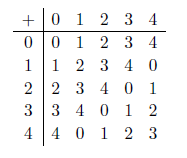
\includegraphics{images/groups_01_1.png}
\caption{Page1}
\end{figure}

The effect of the identitiy element \(0\) can be seen in the first row /
column. Furthermore, \(0\) appears exactely once in every row / column;
therefore there exists an inverse element.

\subsubsection{Example: Integers mod n
Multiplication}\label{example-integers-mod-n-multiplication}

If we consider modulo n multiplication instead, things become different:
The element \(1\) acts as identitiy element \(a \star 1 = a\), but there
is no inverse element for the element \(0\): \(a \star 0 = 0\) for all
\(a\). The way out of this is to remove the element \(0\); i.e.~we
consider \(\mathbb{Z}_n - \{0\}\).

This remedy does not create a group in all cases \(n\) as the following
example shows: The table below shows the multiplication tables for
\(\mathbb{Z}_4 - \{0\}\) and \(\mathbb{Z}_5 - \{0\}\).

\begin{figure}
\centering
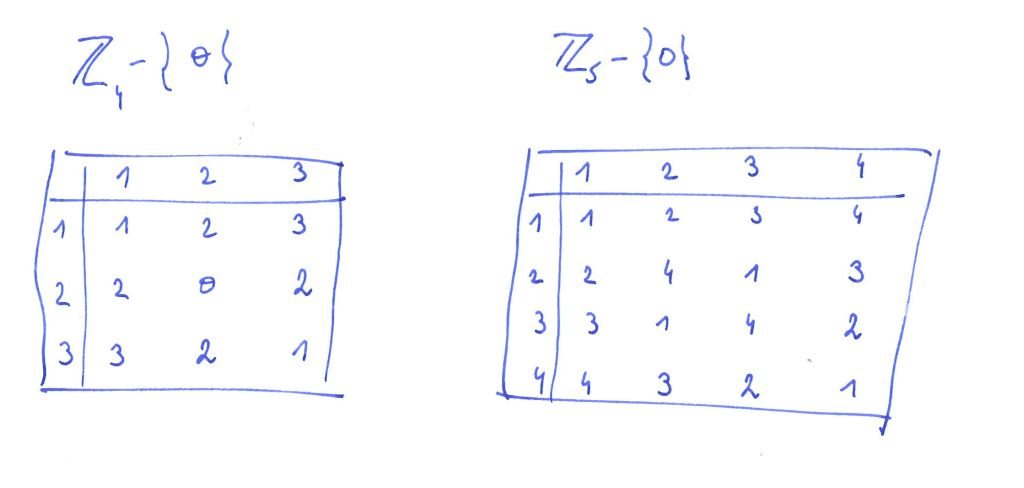
\includegraphics{images/groups_01_2.jpg}
\caption{Page1}
\end{figure}

\(\mathbb{Z}_4 - \{0\}\) has no identitiy element for \(2\); no matter
what \(2\) is multiplied with, the result is never \(1\) (the identity
element). Furthermore, \(0\) is per definition \textbf{not} an element
of \(\mathbb{Z}_4 - \{0\}\). Therefore, \(\mathbb{Z}_4 - \{0\}\) is
\textbf{not} a group. For \(\mathbb{Z}_5 - \{0\}\), every element has an
inverse; therefore this set forms a group (under multiplication module
\(5\)).

There is a proposition, that every nonzero \(k\) has an inverse in
\(\mathbb{Z}_n - \{0\}\), if \(k\) is relatively prime to \(n\). If we
collect all elements \(k \in \mathbb{Z}_n - \{0\}\) which have
\(\gcd(k,n)=1\), we obtain a group, the \textbf{group of units} \(U(n)\)
of \(\mathbb{Z}_n\). Euler's totient function \(\phi(n)\) counts the
integers up to a given number n that are relatively prime to n.
Therefore, the group of units order is \(|U(n)| = \phi(n)\).

As an example consider \(n=8\): The following elements of
\(\mathbb{Z}_8 - \{0\}\) are relatively prime to 8: 1,3,5,7. These
elements form the group of unity \(U(8)\) which multiplication table is
as follows:

\[
\begin{array}{c|cccc}
\star & 1 & 3 & 5 & 7 \\ \hline
1     & 1 & 3 & 5 & 7 \\
3     & 3 & 1 & 7 & 5 \\
5     & 5 & 7 & 1 & 3 \\
7     & 7 & 5 & 3 & 1
\end{array}
\]

Finally, if \(n\) is prime, then all \(k\) are relatively prime to \(n\)
and the set \(\mathbb{Z}_n - \{0\}\) forms a group under multiplication
modulo n. This is the reason why \(\mathbb{Z}_5 - \{0\}\) is a group.

\subsection{Subgroups}\label{subgroups}

A subgroup \(H\) of a group \(H\) is a subset \(H\) of \(G\) such that
when the group operation of \(G\) is restricted to \(H\), \(H\) is a
group in its own right. Every group \(G\) with at least 2 elements has
always two subgroups: the subgroup containing the identity element only
(trivial subgroup) and the group \(G\) itself. Everything in between is
a proper subgroup.

\subsection{Cyclic (Sub)Groups}\label{cyclic-subgroups}

If \(G\) is a group and \(a\) any element of the group. Then the set

\[
\langle a \rangle = \{a^k: k \in \mathbb{Z}\}
\]

is a subgroup of \(G\) and \(\langle a \rangle\) is the smallest
subgroup of \(G\) that contains \(a\).

Note that \(a^k\) denotes repeated (k times) application of the
\(\star\) operation on \(a\). I.e.
\(a^2 = a \star a, a^3 = a \star a \star a \cdots\). If using \(+\) as a
group operation, then \(\langle a \rangle = \{ka: k \in \mathbb{Z}\}\)
will be more intuitive.

Proof: \(k=0 \rightarrow a^0 = e\) creates the identity element which is
in \(\langle a \rangle\). If \(g = a^m\) and \(h = a^n\), then
\(g \star h = a^{m+n} \in \langle a \rangle\) (the subgroup is closed)
and finally, \(a^n \star a^{-n} = e\), i.e.~for every
\(a \in \langle a \rangle\), there exists an inverse element.

There are two options for the relation between \(\langle a \rangle\) and
G:

\begin{itemize}
\item
  \(\langle a \rangle\) is a subgroup of G; in this case
  \(\langle a \rangle\) is called a \textbf{cyclic subgroup} of G.
\item
  \(\langle a \rangle\) = G; i.e.~the complete group G can be created
  via the cyclic operation. In this case, G is called a \textbf{cyclic
  group} and and a is the \textbf{generator} of G.
\end{itemize}

The sequence \(e, a, a^2, a^3, \cdots\) may eventually end in the
identity element \(e\). In this case we speak of finite cyclic
(sub)groups. The order of \(\langle a \rangle\) is the smallest positive
integer n such that \(a^n = e\).

As an example, consider the group \(\mathbb{Z}_5\) (addition module-5).
The element \(1\) is a generator for the group:
\(0 \times 1 = 0, 1 \times 1 = 1, 2 \times 1 = 2, 3 \times 1 = 3, 4 \times 1 = 4, 5 \times 1 = 0\).
Therefore, \(\mathbb{Z}_5\) is a cyclic group with order 5. In the same
spirit, the element \(2\) is also a generator for the group:
\(0 \times 2 = =0, 1 \times 2 = 2, 2 \times 2 = 4, 3 \times 2 = 1, 4 \times 2 = 3, 5 \times 2 = 0\).

The generator \(2\) of the group \(\mathbb{Z}_6\) creates a cyclic
subgroup \(\langle 2 \rangle = \{0, 2, 4\}\) which does not equal the
group. So \(\langle 2 \rangle\) is a cyclic subgroup of order 3.

%\DiaryEntry{Groups, II}{2016-03-03}{Algebra}

In this post, we consider the operation and symmetries of an equilateral
triangle.

\subsubsection{Identity}\label{identity}

The identity transformation leaves the triangle as it is.

\begin{figure}
\centering
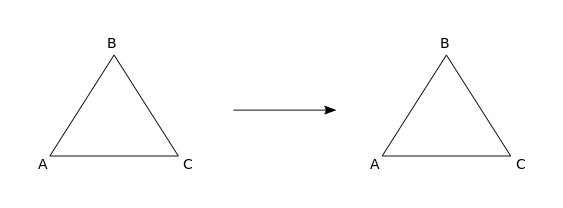
\includegraphics[scale=0.7]{images/groups_02_1.png}
\caption{Page1}
\end{figure}

We can write the effect of the transformation as a permutation matrix of
the points A, B, and C.

\[
e=\begin{pmatrix}
A & B & C\\
A & B & C\end{pmatrix}
\]

\subsubsection{Rotation}\label{rotation}

There are two rotations, clockwise and counter-clockwise possible.

\begin{figure}
\centering
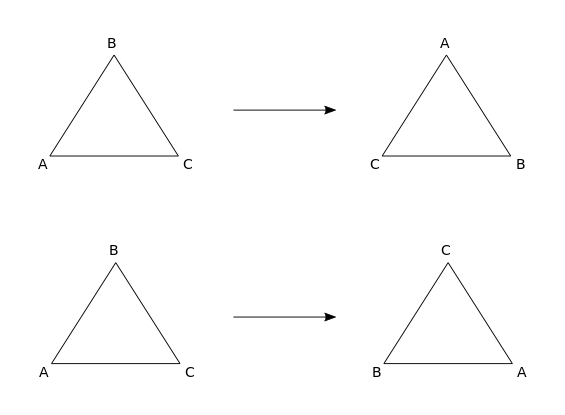
\includegraphics[scale=0.7]{images/groups_02_2.png}
\caption{Page1}
\end{figure}

The clockwise rotation (upper one) has the following permutation matrix:

\[
\rho_1=\begin{pmatrix}
A & B & C\\
B & C & A\end{pmatrix}
\]

Because of the rotation, the point A becomes the point B and so on.

The counter-clockwise rotation (lower one) has the following permutation
matrix:

\[
\rho_2=\begin{pmatrix}
A & B & C\\
C & A & B\end{pmatrix}
\]

\subsubsection{Reflection}\label{reflection}

There ae three reflections possible; each leaving one triangle point the
same.

\begin{figure}
\centering
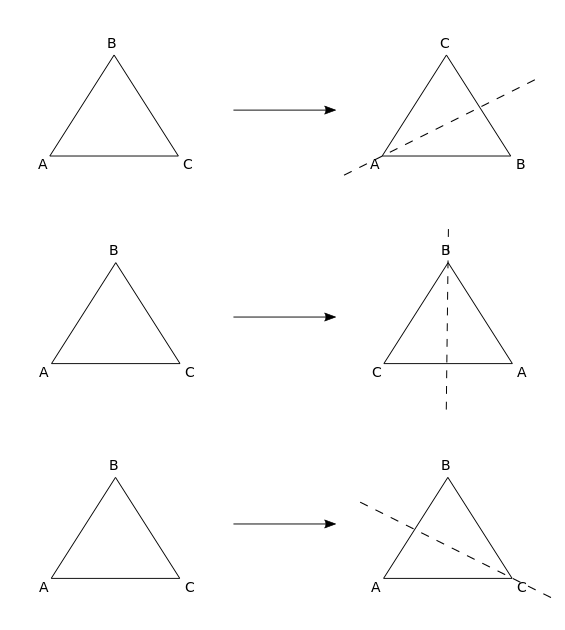
\includegraphics[scale=0.7]{images/groups_02_3.png}
\caption{Page1}
\end{figure}

The first reflection has the following permutation matrix

\[
\mu_1=\begin{pmatrix}
A & B & C\\
A & C & B\end{pmatrix}
\]

The second reflection has the following permutation matrix

\[
\mu_2=\begin{pmatrix}
A & B & C\\
C & B & A\end{pmatrix}
\]

The third reflection has the following permutation matrix

\[
\mu_3=\begin{pmatrix}
A & B & C\\
B & A & C\end{pmatrix}
\]

\subsection{Group Interpretation}\label{group-interpretation}

In total, there are 6 operations for the triangle: 1 ``do-nothing''
identity, 2 rotations, and 3 reflections. These 6 operations form a
group with the function \(\star\) being the combination of two such
permutations: the function is associative, there exists an identity
element (the first ``identity'' permutation above), and there exists an
inverse element (a permutation is a one-to-one mapping; therefore it has
an inverse).

As an example of combination, consider the effect of the subsequent
execution of \(\mu_1\) and \(\rho_1\) on the point A:
\((\mu_1 \rho_1)(A) = \mu_1(\rho_1(A)) = \mu_1(B) = C\). The same for
points B and C yields \((\mu_1 \rho_1)(B) = B\) and
\((\mu_1 \rho_1)(C) = A\). We can again write this as a permutation
matrix

\[
\mu_1 \rho_1 = \begin{pmatrix}
A & B & C\\
C & B & A\end{pmatrix}
\]

and from this we see that the combined effect of the two permutations
equals \(\mu_2\).

\subsubsection{Multiplication Table}\label{multiplication-table}

We can capture the combined effect of two operations / permutations by
means of a multiplication table (the table is to be read ``row-first''):

\[
\begin{array}{c|cccccc}
\star  & e     & \rho_1 & \rho_2 & \mu_1 & \mu_2 & \mu_3 \\
\hline
e     & e     & \rho_1 & \rho_2 & \mu_1 & \mu_2 & \mu_3 \\
\rho_1 & \rho_1 & \rho_2 & e     & \mu_3 & \mu_1 & \mu_2 \\
\rho_2 & \rho_2 & e     & \rho_1 & \mu_2 & \mu_3 & \mu_1 \\
\mu_1  & \mu_1  & \mu_2  & \mu_3  & e    & \rho_1& \rho_2\\
\mu_2  & \mu_2  & \mu_3  & \mu_1  & \rho_2 & e    & \rho_1\\
\mu_3  & \mu_3  & \mu_1  & \mu_2  & \rho_1 & \rho_2& e
\end{array}
\]

We see the combination of \(\mu_1\) and \(\rho_1\) in the row \(\mu_1\)
and column \(\rho_1\) being \(\mu_2\).

From the table we also observe that the group is \textbf{not} abelian as
the oeration is \textbf{not} commutative; e.g.
\(\rho_1 \star \mu_1 \neq \mu_1 \star \rho_1\).

\subsubsection{Other Interpretation /
Subgroups}\label{other-interpretation-subgroups}

A slightly different interpretation is to define a ``start''
configuration e of a triangle and to consider the effects one
transformation has on this start configuration. If we define the start
configuration as the first triangle above, then \(\rho_1\) defines a
clockwise rotation of this triangle. Subsequent transformations can be
grouped into one compound transformation as by the multiplication table
above.

This interpretation allows to investigate the subgroups of the group. We
start with e and repeatedly apply \(\rho_1\), in order to receive the
following sequence: e
\(\rightarrow \rho_1 \rightarrow \rho_2 \rightarrow\) e. In a similar
spirit we obtain e \(\rightarrow \mu_1 \rightarrow\) e, e
\(\rightarrow \mu_2 \rightarrow\) e, and e
\(\rightarrow \mu_3 \rightarrow\) e.

Each of these subgroups is cyclic; however, no single element generates
the whole group, therefore the whole group is not cyclic. The Figure
below shows these cyclic subgroups.

\begin{figure}
\centering
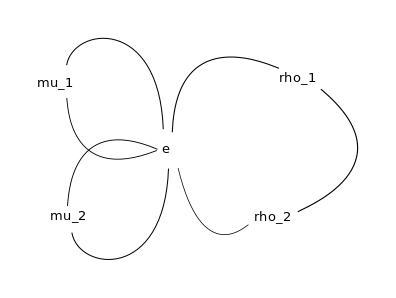
\includegraphics[scale=0.7]{images/groups_02_4.png}
\caption{Page1}
\end{figure}

\subsubsection{Relation to Permutation
Groups}\label{relation-to-permutation-groups}

In this special case of triangles, the 6 operations represent all
permutations of the three triangle points A, B, C. Therefore, the group
we described above is actually the permutation group \(S_3\).

Permutations are covered in a later post (Groups, IV).


%\DiaryEntry{Groups, III}{2016-03-04}{Algebra}

\subsection{Cyclic Groups}\label{cyclic-groups}

Cyclic groups are denoted as \(C_n\) and are defined by
\(G =\langle a \rangle\) where \(a\) is the \textbf{generator} of G.

Simplest examples for cyclic groups are the integers with modulo-n
addition; i.e. \(\mathbb{Z}_n\).

The following Figure shows Cayley diagrams for \(n=3\) and \(n=5\).

\begin{figure}[H]
\centering
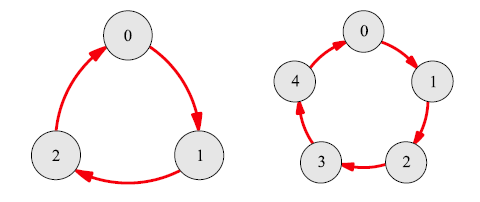
\includegraphics{images/groups_03_1.png}
\caption{Page1}
\end{figure}

The left diagram shows the group elements \(1,2,3\) and the effect the
operation \((x + 1) \mod 3\) has on each group element as the red lines
(with arrows). Note that selecting another operation (e.g.
\((x + 2) \mod 3\)) would make the lines look different.

The right figure shows the same for the group elements \(1,2,3,4,5\) and
operation \((x + 1) \mod 5\).

Another example for a cyclic group are the (complex) roots of unity
under (complex) multiplication; i.e.

\[
x_k = \exp \frac{2\pi i}{N} k, \quad k=0,\ldots,N-1
\]

We have that \(x_k x_k\) is an element of the group and the identity
element is \(1\). Therefore, the elements \(x_k\) for a group.
Furthermore, the group is cyclic with generator being \(x_1\).

\subsection{Permutation Groups}\label{permutation-groups}

The permutations of a set form a group; if the set is the numbers from
1\ldots{}n, the group is the symmetric group \(S_n\). The group has
\(n!\) elements and the binary operation is the composition of
permutations. Note that permutations are not commutative in general.

A permutation group has several subgroups; as an example consider the
subgroup of \(G_5\) consisting of the identitiy element and the
following elements

\[
\sigma =
\begin{pmatrix}
1 & 2 & 3 & 4 & 5 \\
1 & 2 & 3 & 5 & 4
\end{pmatrix}
,\quad \tau = 
\begin{pmatrix}
1 & 2 & 3 & 4 & 5 \\
3 & 2 & 1 & 4 & 5
\end{pmatrix}
, \quad \mu = 
\begin{pmatrix}
1 & 2 & 3 & 4 & 5 \\
3 & 2 & 1 & 5 & 4
\end{pmatrix}
\]

The following table shows how to multiply elements in this subgroup:

\[
\begin{array}{c|cccc}
\star   & e     & \sigma & \tau   & \mu    \\
\hline
e     & e     & \sigma & \tau   & \mu    \\
\sigma & \sigma & e     & \mu    & \tau   \\
\tau   & \tau   & \mu    & e     & \sigma \\
\mu    & \mu    & \tau   & \sigma & e
\end{array}
\]

\subsubsection{Cycle Notation}\label{cycle-notation}

This is a shorthand notation for writing permutations. The cycle
notation lists all cycles of a permutation. For example, the permutation
\(\sigma\) is in cycle notation \((4,5)\), for \(\tau\) it is \((1,3)\),
and for \(\mu\) it is \((1,3)(4,5)\). Elements which are not part of a
cycle are not listed; that is the elements \(1,2,3\) are left in place
by the permutation \(\sigma\). Besides, note that permutations can also
contain more than one cycle.

As another example consider the permutation

\[
\begin{pmatrix}
1 & 2 & 3 & 4 & 5 & 6 \\
2 & 4 & 1 & 3 & 6 & 5
\end{pmatrix}
\]

which has cycle notation \((1,2,4,3)(5,6)\). Note that the order of the
elements in the cycle is important; i.e.~cycles \((1,2,4,3)\) and
\((1,2,3,4)\) denote different cycles.

\subsubsection{More on Cylces}\label{more-on-cylces}

Cycles can be multiplied; for example if we have \(\sigma=(1,3,5,2)\)
and \(\tau = (2,5,6)\), then the product \(\sigma \tau\) can be obtained
by considering the effect of \(\sigma \tau\) on every integer: We have
\(\sigma (\tau (1)) = \sigma(1) = 3\),
\(\sigma (\tau (2)) = \sigma(5) = 2\),
\(\sigma (\tau (3)) = \sigma(3) = 5\),
\(\sigma (\tau (4)) = \sigma(4) = 4\),
\(\sigma (\tau (5)) = \sigma(6) = 6\),
\(\sigma (\tau (6)) = \sigma(2) = 1\). Converting this into cycle
notation, we obtain for the product \(\sigma \tau = (1,3,5,6)\)

Two cycles are disjoint if they contain different elements. If
\(\sigma\) and \(\tau\) are disjoint cycles, then
\(\sigma \tau = \tau \sigma\).

Proof: For elements in neither cycle, both \(\sigma\) and \(\tau\) leave
these elements untouched, therefore order of permutations is not
important. If an element is contained in one cycle it is not contained
in the other cycle (by definition of disjointness) and therefore not
touched by this permutation.

Assume that \(a\) is contained in \(\sigma\), but not in \(\tau\).
Therefore \(\tau(a) = a\) and \(\sigma(\tau(a)) = \sigma(a)\) and
\(\tau(\sigma(a)) = \sigma(a)\). The argument stays the same when \(a\)
is contained in \(\tau\) instead.

Every permutation in \(S_n\) can be expressed as product of disjoint
cycles.

A transposition is a cylce of length 2; i.e.~an element exchange. Any
permutation of finite elements with at least 2 elements can be written
as product of transpositions (not necessarily disjoint).

As an example, consider the product of
\(\sigma_1 \sigma_2 = (2,4)(2,6)\). We need only to consider what
happens to the element \(2,4,6\) as all other elements are outside the
cycle(s). Therefore, we have \(\sigma_1(\sigma_2(2)) = 6\),
\(\sigma_1(\sigma_2(4)) = 2\), \(\sigma_1(\sigma_2(6)) = 4\). Combining
this into a cycle yields \((2,6,4)\). From this we deduce the general
rule that

\[
(a,b)(a,c) = (a,c,b), \quad \mbox{and} \quad (a,b)(a,c)(a,d) = (a,d,c,b)
\]

There is no unique way of writing permutations as product of
transpositions; however, the number of transpositions to express a
permutation is a constant. We define a permutation to be \textbf{even},
if it can be expressed as an even number of transpositions and
\textbf{odd} if it can be expressed as an odd number of transpositions.

\subsection{Alternating Groups}\label{alternating-groups}

One of the most important subgroups of \(S_n\) is the set of all even
permutations, \(A_n\), the alternating group on n elements. \(A_n\) is a
subgroup of \(S_n\).

%\DiaryEntry{Sum of Gaussian RVs}{2016-03-07}{Stochastic}


Consider two Gaussian RVs \(X_1, X_2\) with distributions
\(f_1(x) = \mathcal{N}(x, \mu_1, \sigma_1^2)\) and
\(f_2(x) = \mathcal{N}(x, \mu_2, \sigma_2^2)\), respectively.

The RV \(S\) denotes their sum; \(S = X_1 + X_2\) and we want to
calculate the distribution \(f(x)\) of \(S\).

In general, the pdf of the sum of two RVs is the convolution of their
pdfs; i.e.

\[
f(x) = \int_{-\infty}^\infty f_1(u) f_2(x-u) du
\]

For a fixed value \(x\), we sum over all probability contributions from
\(X_1\) and \(X_2\) to this \(x\).

In the cae of Gaussian RVs, we have

\[
f(x) = \int_{-\infty}^\infty \frac{1}{\sqrt{2\pi\sigma_1^2}} \exp{- \frac{(u-\mu_1)^2}{2\sigma_1^2}} \frac{1}{\sqrt{2\pi\sigma_2^2}} \exp{- \frac{(x - u-\mu_2)^2}{2\sigma_2^2}} du
\]

\subsection{Special Case: Zero-mean, same Variance}

To get started, simplify things and consider \(\mu_1 = \mu_2 = 0\) and
\(\sigma_1^2 = \sigma_2^2 = \sigma^2\). Then we have

\begin{align*}
f(x) &= \frac{1}{\sqrt{4\pi^2\sigma_2^4}} \int_{-\infty}^\infty  \exp{- \frac{u^2}{2\sigma^2} - \frac{(x-u)^2}{2\sigma^2}} du = \frac{1}{\sqrt{4\pi^2\sigma_2^4}} \int_{-\infty}^\infty  \exp{- \frac{u^2 + (x-u)^2}{2\sigma^2}} du \\ &= \frac{1}{\sqrt{4\pi^2\sigma_2^4}} \int_{-\infty}^\infty  \exp{- \frac{2u^2 - 2xu + x^2}{2\sigma^2}} du
\end{align*}

Completing the square in the exponential, we obtain

\[
2u^2 - 2xu + x^2 = \left(\sqrt{2}u - \frac{1}{\sqrt{2}}x\right)^2 + \frac{1}{2}x^2
\]

and we obtain

\begin{align*}
f(x) &= \frac{1}{\sqrt{4\pi^2\sigma_2^4}} \int_{-\infty}^\infty  \exp{- \frac{\left(\sqrt{2}u - \frac{1}{2}x\right)^2 + \frac{1}{2}x^2}{2\sigma^2}} du \\ &= \frac{1}{\sqrt{4\pi^2\sigma_2^4}} \int_{-\infty}^\infty \exp{- \frac{ \left(\sqrt{2}u - \frac{1}{\sqrt{2}} x\right)^2}{2\sigma^2}} \exp{- \frac{\frac{1}{2}x^2}{2\sigma^2}} du
\end{align*}

We can pull the last exp term in front of the integral and arrive at

\[
f(x) = \frac{1}{\sqrt{4\pi^2\sigma_2^4}} \exp{\left(- \frac{x^2}{4\sigma^2} \right)} \int_{-\infty}^\infty \exp{- \frac{ \left(\sqrt{2}u - \frac{1}{\sqrt{2}} x\right)^2}{2\sigma^2}} du
\]

For the integral, we use the fact that the integral over a Gaussian
distribution is one; i.e.

\[
\frac{1}{\sqrt{2\pi\sigma^2}} \int_{-\infty}^\infty \exp{- \frac{ (x-\mu)^2 }{2\sigma^2}} du = 1 \rightarrow \int_{-\infty}^\infty \exp{- \frac{ (x-\mu)^2 }{2\sigma^2}} du = \sqrt{2\pi\sigma^2}
\]

\textbf{independent} of the value \(\mu\). Therefore we have

\begin{align*}
f(x) &= \frac{1}{\sqrt{4\pi^2\sigma_2^4}} \exp{\left(- \frac{x^2}{4\sigma^2} \right)} \int_{-\infty}^\infty \exp{- \frac{ 2 \left(u - c x\right)^2}{2\sigma^2}} du \\ &= \frac{1}{\sqrt{4\pi^2\sigma_2^4}} \exp{\left(- \frac{x^2}{4\sigma^2} \right)} \int_{-\infty}^\infty \exp{- \frac{ \left(u - c x\right)^2}{2\sigma^2 / 2}} = \frac{1}{\sqrt{4\pi^2\sigma_2^4}} \exp{\left(- \frac{x^2}{4\sigma^2} \right)} \sqrt{2\pi\sigma^2 / 2}
\end{align*}

where \(c\) is a constant (I'm too lzay to calculate as it's not
important anyway).

Bringing this into a nicer form, we can see what's going on

\[
f(x) = \frac{1}{\sqrt{2\pi2\sigma^2}} \exp{\left(- \frac{x^2}{2 \cdot 2 \sigma^2} \right)} 
\]

We have a Gaussian RV with zero-mean and variance \(2\sigma^2\) - as
expected!

%\DiaryEntry{Groups, Dihedral Groups}{2016-03-15}{Algebra}

These groups \(D_n\) represent the rigid motions of a regular n-sided
polygon. These groups have order \(2n\). We define a clockwise rotation
operation \(r\) as follows:

\begin{figure}[H]
\centering
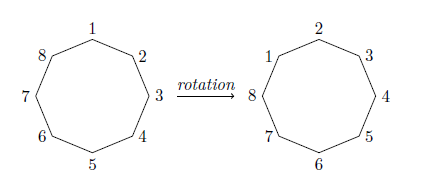
\includegraphics[scale=0.7]{images/groups_04_1.png}
\caption{Page1}
\end{figure}

And we define a reflection operation \(s\) as in the Figure below
(depending on \(n\) being even or odd, the reflection operation leaves
one or two points unchanged).

\begin{figure}[H]
\centering
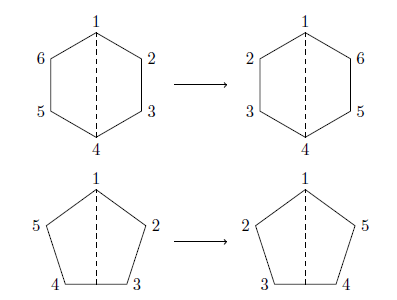
\includegraphics[scale=0.7]{images/groups_04_2.png}
\caption{Page1}
\end{figure}

With these two operations, a Diheadral group \(D_n\) is defined as all
products of the two elements \(r\) and \(s\) which satisfy the following
conditions:

\begin{align*}
r^n &= 1 \\
s^2 &= 1 \\
srs &= r^{-1}
\end{align*}


The first condition states, that after \(n\) rotations all polygon
points are back at their original position. The second condition states
that two reflections leave all polygon points unchanged. FInally, the
third condition states, that reflection, rotation, and a reflection is
the same as rotation in the inverse direction.

Note that \(r\) and \(s\) are used to define the group elements; but
\(D_n\) consists of more elements than these two; namely all products
fulfilling above conditions.

\subsection{Example $D_4$}

This group has \(2n = 2 \dot 4 = 8\) elements. The identity element
\(e\), 3 rotations \(r, r^2, r^3\), one reflection \(s\) and 3 rotations
preceded by a reflection \(rs, r^2s, r^3s\). The choice of the last
three elements is somewhat arbitrary (we could have used
\(sr, sr^2, sr^3\)), but choosing it this way is consistent with
\href{http://groupprops.subwiki.org/wiki/Dihedral_group:D8}{this
internet ressource} and the book ``Visual Group Theory'').

The elements are shown in the Figure below.

\begin{figure}[H]
\centering
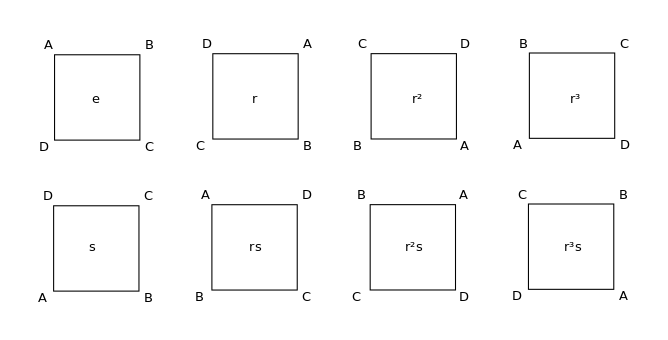
\includegraphics[scale=0.7]{images/groups_04_3.png}
\caption{Page1}
\end{figure}

First note that the group is \textbf{not} abelian.

The multiplication table shall describe the relation between these 8
elements; e.g.~what is the result of \(r^3s \star rs\). This can be
simply written as \(r^3srs\) but this expression is not in the form of
one of the 8 group elements. In order to achieve this, we need to
simplify the resulting expressions so that they equal one of the
elements.

The following multiplication table shows the results of multiplying
elements without simplifying the result. All results in red need further
simplification.

\[
\begin{array}{c|cccccccc}
\star   & 1    & r & r^2  & r^3 & s & rs & r^2s & r^3s \\
\hline
1 & 1 & r & r^2 & r^3 & s & rs & r^2s & r^3s \\
r & r & r^2 & r^3 & 1 & rs & r^2s & r^3s  & s \\
r^2 & r^2 & r^3 & 1 & r & r^2 s & r^3s & s & rs \\
r^3 & r^3 & 1 & r & r^2 & r^3s & s & rs & r^2s \\
s  &  s & \color{red}{sr} & \color{red}{sr^2} & \color{red}{sr^3} & e & \color{red}{srs}  & \color{red}{sr^2s} & \color{red}{sr^3s} \\
rs & rs & \color{red}{rsr} & \color{red}{rsr^2} & \color{red}{rsr^3} & r & \color{red}{rsrs}  & \color{red}{rsr^2s} & \color{red}{rsr^3s} \\
r^2s & r^2s & \color{red}{r^2sr} & \color{red}{r^2sr^2} & \color{red}{r^2sr^3} & r^2 & \color{red}{r^2srs}  & \color{red}{r^2sr^2s} & \color{red}{r^2sr^3s} \\
r^3s & r^3s & \color{red}{r^3sr} & \color{red}{r^3sr^2} & \color{red}{r^3sr^3} & r^3 & \color{red}{r^3srs} & \color{red}{r^3sr^2s} & \color{red}{r^3sr^3s}
\end{array}
\]

In order to simplify the red entries, we observe the following
equalities:

\begin{itemize}
\item
  Start with \(srs = r^{-1}\), left-multiply both sides with \(s\) and
  obtain \(s^2rs = s r^{-1}\) which becomes \(rs = s r^{-1}\).
  Righ-multiplying with \(r\) finally yields \(rsr = s\).
\item
  We have \(sr = r^3 s\): Multiplying on the left with \(r\), we obtain
  \(rsr = r^4 s = r^3\). From the definitions above, we have \(s = s\)
  which is true.
\item
  We have \(sr^2 = r^2s\): Left-multiplying with \(r\) yields
  \(rsr^2 = r^3s\) which we can simplify to \(sr = r^3s\) which was
  proven above.
\item
  We have \(srs = r^{-1}\). Multiplying both sides with \(r^4 = 1\), we
  obtain \(srs = r^3\).
\end{itemize}

The table below shows the simplified expressions based on the identites
above.

\[
\begin{array}{c|cccccccc}
\star   & 1    & r & r^2  & r^3 & s & rs & r^2s & r^3s \\
\hline
1 & 1 & r & r^2 & r^3 & s & rs & r^2s & r^3s \\
r & r & r^2 & r^3 & 1 & rs & r^2s & r^3s  & s \\
r^2 & r^2 & r^3 & 1 & r & r^2 s & r^3s & s & rs \\
r^3 & r^3 & 1 & r & r^2 & r^3s & s & rs & r^2s \\
s  &  s & \color{red}{sr} = r^3s & \color{red}{sr^2} = r^2s & \color{red}{sr^3} = r^2 s r = rs & 1 & \color{red}{srs} = r^3  & \color{red}{sr^2s} = r^2ss = r^2& \color{red}{sr^3s} = ssr = r\\
rs & rs & \color{red}{rsr} = s & \color{red}{rsr^2} = sr = r^3s& \color{red}{rsr^3} = r^2s& r & \color{red}{rsrs} = s^2 = 1  & \color{red}{rsr^2s} = r r^2s s = r^3& \color{red}{rsr^3s} = rs sr = r^2\\
r^2s & r^2s & \color{red}{r^2sr} = rs & \color{red}{r^2sr^2} = r s r = s& \color{red}{r^2sr^3} = r^2 rs = r^3s& r^2 & \color{red}{r^2srs} = r  & \color{red}{r^2sr^2s} = r^2 r^2s s = 1& \color{red}{r^2sr^3s} = r^2ssr = r^3\\
r^3s & r^3s & \color{red}{r^3sr} = r^2s & \color{red}{r^3sr^2} = r^2 rsr r = r^2 s r = rs & \color{red}{r^3sr^3}= r^3 rs = s & r^3 & \color{red}{r^3srs} = r^2& \color{red}{r^3sr^2s} = r^3 r^2ss = r& \color{red}{r^3sr^3s} = r^3ssr = 1
\end{array}
\]

Finally, the table below shows the multiplication table for the dihedral
group \(D_4\):

\[
\begin{array}{c|cccccccc}
\star   & 1    & r & r^2  & r^3 & s & rs & r^2s & r^3s \\
\hline
1 & 1 & r & r^2 & r^3 & s & rs & r^2s & r^3s \\
r & r & r^2 & r^3 & 1 & rs & r^2s & r^3s  & s \\
r^2 & r^2 & r^3 & 1 & r & r^2 s & r^3s & s & rs \\
r^3 & r^3 & 1 & r & r^2 & r^3s & s & rs & r^2s \\
s  &  s & r^3s & r^2s & rs & 1 & r^3  & r^2& r\\
rs & rs & s & r^3s& r^2s & r & 1  & r^3 & r^2\\
r^2s & r^2s & rs & s & r^3s & r^2 & r & 1 & r^3\\
r^3s & r^3s & r^2s & rs & s & r^3 & r^2 & r&  1
\end{array}
\]

The following Figure shows the corresponding Cayley diagram: Red lines
correspond to multiplication with \(r\) and blue lines correspond to
multiplication with \(s\). Since \(s^2 = 1\) the orientation of the blue
lines does \textbf{not} matter: Following a blue line in any direction
\textbf{always} corresponds to multiplication by \(s\) (This is contrary
to multiplication with \(r\) where the direction \textbf{is} important).

Note also that the Cayley diagram uses the (rather unusual) convention
that multiplication is interpreted from left to right; i.e.
\(A \star B\) corresponds to starting in point B, follow the line
corresponding to multiplication with A. This can be seen in the right
part: When we start at \(r\) and follow the blue line to the inner
circle, we land at the point \(sr\) (which is equivalent to \(r^3s\)).

\begin{figure}[H]
\centering
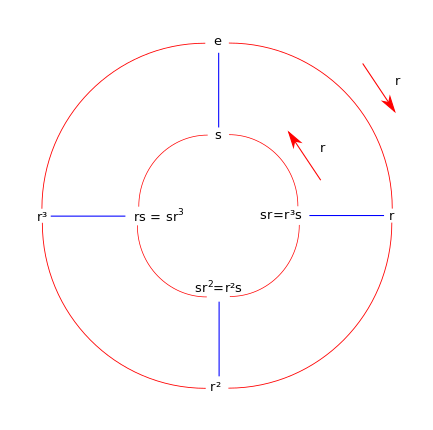
\includegraphics[scale=0.7]{images/groups_04_4.png}
\caption{Page1}
\end{figure}

Using the more common convention that \(AB\) corresponds to starting at
\(A\) and follow the line corresponding to multiplication with \(B\), we
arrive at the Cayle diagram shown below. Again looking at the right part
of the Figure, when we start at \(r\) and follow the blue line to the
inner circle, we land at the point \(rs\).

\begin{figure}[H]
\centering
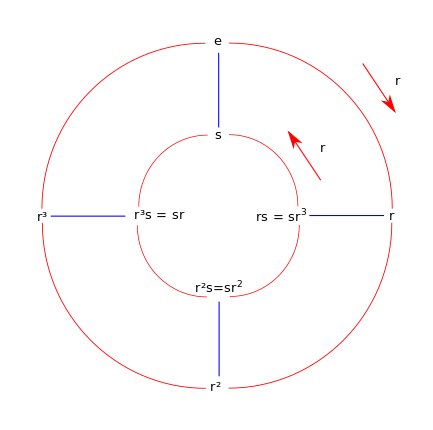
\includegraphics[scale=0.7]{images/groups_04_5.png}
\caption{Page1}
\end{figure}

\subsubsection{\texorpdfstring{Relation with
\(S_4\)}{Relation with S\_4}}\label{relation-with-s_4}

Contrary to the rigid motions of the triangle (which were equivalent
with \(S_3\)), the group \(D_4\) (and all other groups \(D_n\) with
\(n > 3\)) is a subgroup of \(S_4\). Put another way, \(D_4\) does not
contain all permutations of \(4\) elements like \(S_4\) does. The Figure
below shows 2 missing permutations: the left one is created by twisting
the square along the x-axis; the right one is created by twisting along
the y-axis. Each of these 2 permutations can be rotated and reflected in
8 differerent ways (like discussed above), giving rise to additional
\(2 \times 8 = 16\) elements. Therefore we have \(8 + 16 = 24 = 4!\)
elements; the same number of \(S_4\) has.

\begin{figure}
\centering
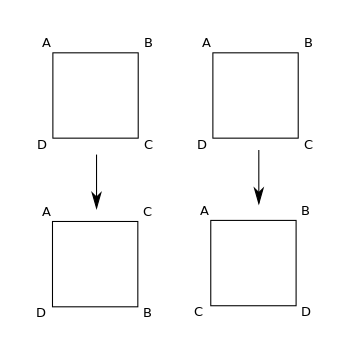
\includegraphics[scale=0.7]{images/groups_04_6.png}
\caption{Page1}
\end{figure}

%\DiaryEntry{Groups - Cosets}{2016-03-25}{Algebra}

Consider a groupg G with a subgrop H; A left coset of H with
representative \(a \in G\) is defined as

\[
aH = \{a \star h: h \in H \}
\]

That is, we choose \textbf{any} element a from G and create the set by
performing the group operation \(\star\) on a and every element from H.

Since the group operation is not commutative in general, we can
analoguously define a right coset according to

\[
Ha = \{h \star a : h \in H \}
\]

Note that cosets are sets and \textbf{not} groups.

\subsection{Example $\mathbb{Z}_6$}\label{example-mathbbz_6}

Consider the group \(G = \mathbb{Z}_6\) with element \(0,1,2,3,4,5\) and
modulo-6 addition as group operation. The subgroup is \(H = \{0,3\}\).

Make a quick check that H is really a subgroup: (i) It contains the
identitiy element \(0\), (ii) it is closed under addition modulo-6 as
\(3 \star 3 = 0\), and (iii) every group element has an inverse:
trivially for group element \$0\$0, and the inverse of \(3\) is \(3\);
see (ii).

Since the group operation is commutative, left and right cosets are the
same; we have

\begin{align*}
0 + H &= \{0,3\} \\
1 + H &= \{1,4\} \\
2 + H &= \{2,5\} \\
3 + H &= \{3,0\} \\
4 + H &= \{4,1\} \\
5 + H &= \{5,2\}
\end{align*}


First note that several cosets are equal (as cosets are sets, they are
equal when they contain the same elements). Simplifying things we obtain


\begin{align*}
0 + H &= 3 + H = \{0,3\} \\
1 + H &= 4 + H = \{1,4\} \\
2 + H &= 5 + H = \{2,5\} \\
\end{align*}


The Figure below shows the corresponding Cayley diagram with G (black)
and H (red), and the cosets. The cosets have the original structure of
the underlying subgroup; however they are ``shifted'' to a new posiiton.
The Figure and the example above also show that cosets are not groups in
general; e.g.~the coset \(\{1,4\}\) is a set but not a group.

\begin{figure}[H]
\centering
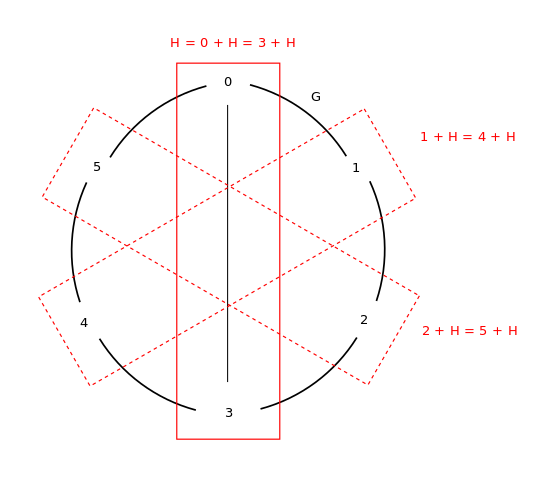
\includegraphics[scale=0.7]{images/groups_05_1.png}
\caption{Page1}
\end{figure}

Since cosets are sets, two cosets \(Ha\) and \(Hb\) are equal when
\(a \in H b\) follows from \(a \in H a\) and vice versa.

\subsection{Coset Characteristics}\label{coset-characterisitcs}

\subsubsection{Coset Membership}\label{coset-membership}

We have the following fact:

\[
a \in Hb \rightarrow Ha = Hb
\]

Let \(x \in Ha\); therefore we have \(x = h_2 a\) where \(h_2\) is some
element of H. But we also have that \(a \in Hb\) which implies that
\(a = h_1 b\) and if we combine that, we get
\(x = h_2 a = h_2 ( h_1 b) = (h_2 h_1) b\). The product \(h_2 h_1\) is
clearly an element of \(H\); therefore \(x \in Hb\). This proves that
every \(x \in Ha\) is also contained in \(Hb\); if we make the same
argument with exchanged roles, we also find that every \(x \in Hb\) is
also contained in \(Ha\).

From this follows that cosets are either disjoint or equal (contain the
same elements). There is no thing as two cosets having only some
elements in common ``ganz oder gar nicht''.

\subsubsection{Coset Partitioning}\label{coset-partitioning}

We have the following theorem: The family of all cosets \(Ha\), as a
ranges of G, is a partition of G.

In the exmaple above, the three cosets \(0 + H, 1 + H, 2 + H\) partition
the group G.

We can prove this in two steps: First we show that two cosets Ha and Hb
are either disjoint or equal. If they are disjoint then we are done. If
not, then choose \(x \in Ha \cap Hb\). From \(x \in Ha\) follows
\(x = h_1 a\) and from \(x \in Hb\) follows \(x = h_2 b\). We can equal
these two and arrive at \(h_1 a = h_2 b\) which we can solve for a as
\(a = (h_1^{-1} h_2) b\). This shows that \(a \in Hb\) (\(h_1^{-1} h_2\)
is clearly an element of H) and from the reasoning in the previous
Subsection, it follows that \(Ha = Hb\).

Second part of the proof is that \textbf{every} element of G is
contained in one of the cosets of H. Choose \(c \in G\) and we can write
this as \(c = c1\) and \(1 \in H\) (otherwise H would not be a
subgroup!). Therefore, \(c = Hc\) and we are done.

\subsubsection{Coset Size}\label{coset-size}

Next we show that all cosets (of a given subgroup H) have the same size
as the subgroup H. Stated differently, there is a one-to-one
correspondence from H to Ha.

We choose the function \(f:H \rightarrow Ha\) as \(f(h) = ah\); here a
remains fixed and h varies. This function is both injective and
surjective:

\begin{itemize}
\item
  It is injective (i.e.~it never maps distinct values \(h\) into the
  same values \(f(h)\)), because if \(f(h_1) = f(h_2)\), then
  \(ah_1 = ah_2\) and therefore \(h_1 = h_2\).
\item
  It is surjective (i.e.~no element from the image is left out), because
  every element of the image Ha can be expressed as \(ha\) (with some
  \(h \in H\)).
\end{itemize}

\subsubsection{Lagrange's Theorem}\label{lagranges-theorem}

We can combine what we have so far: We have a group G and a subgroup H.
G is partitioned by the cosets of H and all these cosets have the same
size. Therefore, the number of elements in G equals the number of
elements in H (or any coset of H) times the number of distinct cosets of
H.

Stated differently, we can say that the order of any subgroup H of a
group G divides the order of G.

If we think of the example above, \(\mathbb{Z}_6\) has 6 elements and
can therefore have subgoups of size 2 and 3.

In the special case of a group with prime order p, only subgroups of
size 1 and p exist. The latter is the group itself. Therefore, a group
with prime order has p subgroups each having order 1. Such a (sub)group
is a cyclic group; and G is then also a cyclic group. Furthermore, any
group element \(a \in G\) forms a cyclic group with equals G with \(a\)
being the generator: \(\langle a \rangle = G\) for any \(a \in G\).

\subsection{Left and Right Cosets, Normal
Subgroups}\label{left-and-right-cosets-normal-subgroups}

A left coset is defined as

\[
aH = \{a \star h: h \in H \}
\]

The interpretation is as follows: We start at the coset
``representative'' \(a\), multiply each subgroup element and the result
forms the left coset.

A right coset is defined as

\[
Ha = \{h \star a : h \in H \}
\]

and can be interpreted that we start in an element of the subgroup
\(H\), and multiply with \(a\). Doing this for all elements of \(H\)
yields the right coset.

The Figure below shows the concepts. The left coset (shown on the left
:-) ) shows the subgroup \(H\) ``surrounding'' the identity element
\(e\). Considering the left coset \(aH\) means shifting every subgroup
element of \(H\) by the element \(a\).

The right coset (shown on the right) starts with the subgroup \(H\):
Every element of the subgroup (which includes the identity element
\(e\)) is then shifted by \(a\), yielding the coset
\(Hg = \{g, h_1 a, h_2 a, h_3 a, \ldots\}\).

\begin{figure}[H]
\centering
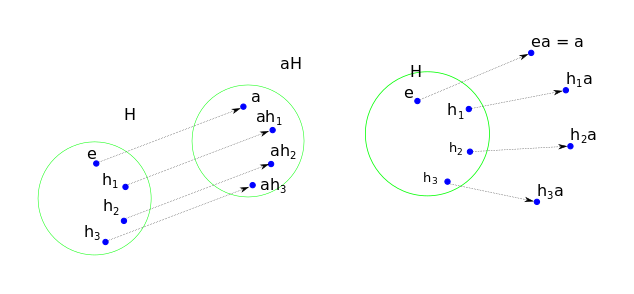
\includegraphics[scale=0.7]{images/groups_05_2.png}
\caption{Page1}
\end{figure}

\subsubsection{Example: Dihedral Group $D_3$}\label{example-dihedral-group-d_3}

In order to beat the examples to death, we consider the Dihedral Group
\(D_3\), defined by the three characteristic equations
\(r^3 = e, s^2=1, srs=r^{-1}\). We use the convention that the operation
\(a\star b\) is to be read from left to right = We start at element a
and apply b.

In the Cayley Diagram shown below, the identities at the points A and B
are interesting. In A, we have \(r^2 s = sr\): Right-multiplying with
\(s\), we obtain \(r^2 s^2 = srs \rightarrow r^2 = r^{-1}\). In B, we
have \(sr^2 = rs\); left-multiplying with \(s\) we obtain
\(s^2 r^2 = srs \rightarrow r^2 = r^{-1}\).

\begin{figure}[H]
\centering
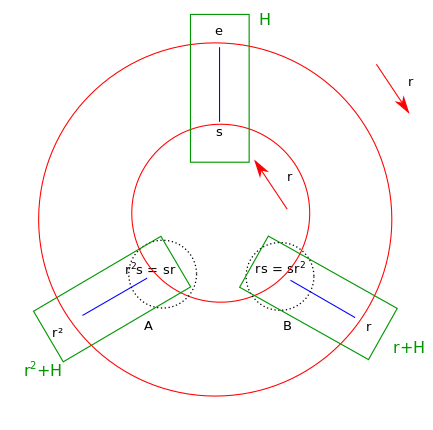
\includegraphics[scale=0.7]{images/groups_05_3.png}
\caption{Page1}
\end{figure}

Next we need a subgroup - the set \(H=\{e, s\}\) is one (as \(s^2=e\)).
The left cosets of \(H\) are

\begin{itemize}
\item
  \(rH = \{re, rs\} = \{r, rs\}\)
\item
  \(r^2H = \{r^2e, r^2s\} = \{r^2, r^2s\}\)
\item
  \(sH = \{s, s^2\} = \{e, s\} = H\)
\item
  \(rsH = \{rs, rs^2\} = rH\)
\item
  \(r^2sH = \{r^2s, r^2s^2\} = r^2H\)
\end{itemize}

The right cosets of \(H\) are

\begin{itemize}
\item
  \(Hr = \{er, sr\} = \{r, sr\}\)
\item
  \(Hr^2 = \{er^2, sr^2\} = \{r^2, sr^2\}\)
\item
  \(Hs = \{s, s^2\} = H\)
\item
  \(Hrs = \{rs, srs\} = \{rs, r^2\} = Hr^2\)
\item
  \(Hr^2s = \{r^2s, sr^2s\} = \{r^2s, r\} = Hr\)
\end{itemize}

It can be seen that the left cosets (shown in green) preserve the
structure of the subgroup, whereas the right cosets distribute elements
across the Cayley diagram.

Next we consider a different subgroup \(H' = \{e, r, r^2\}\). The left
cosets are

\begin{itemize}
\item
  \(rH' = \{r, r^2, e\} = H'\)
\item
  \(r^2H' = \{r^2, e, r\} = H'\)
\item
  \(sH' = \{s, sr, sr^2\}\)
\item
  \(rsH' = \{rs, rsr, rsr^2\} = \{rs, s, sr^2\} = sH'\)
\item
  \(r^2sH' = \{r^2s, r^2sr, r^2sr^2\} = \{r^2s, sr^2, s\} = sH'\)
\end{itemize}

The right cosets are

\begin{itemize}
\item
  \(H'r = \{r, r^2, r^3\} = rH'\)
\item
  \(H'r^2 = \{r^2, e, r\} = r^2H'\)
\item
  \(H's = \{s, rs, r^2s\} = sH'\)
\item
  \(H'rs = \{rs, r^2s, r^3s\} = rsH'\)
\item
  \(H'r^2s = \{r^2s, r^3s, r^4s\} = r^2sH'\)
\end{itemize}

Note that the left and right cosets are equal; therefore, the subgroup
H' is a normal subgroup.

%\DiaryEntry{Groups - Subgroups}{2016-03-29}{Algebra}

Let G be a group and we select a number of group elements. Define S to
be the subset of G containing all possible group operations between
these elements and their inverses, in any order, and with repetition
allowed. Then S is a subgroup of G.

Select three elements and call them a,b, and c. Then e.g.
\(ab, abc, a^2bc, a^{-1}b a c^2 \in S\). We say that the subgroup S has
generators \(a, b, c\).

In the sepcial case of selecting one element, we obtain cyclic groups
which are denoted by \(G = \langle a \rangle\) where a is the
corresponding generator. The combination of operations with \(a\) and
\(a^{-1}\) becomes simple, as e.g. \(a a^{-1}\) cancel each other out.
Therefore, the cyclic group \(G = \langle a \rangle\) contains

\[
\cdots a^{-2}, a^{-1}, 1, a, a^2 \cdots
\]

\subsection{Cayley Diagrams}\label{cayley-diagrams}

Every finite group can be represented by a Cayley diagram: there is one
point for every element in the group. The arrows represent the result of
multiplying by a generator. In case there are several generators, the
arrows need to encode the information which operator is used (e.g.~by
chossing different colors).

That is, a Cayley diagram shows the effect of multiplying two elements
\(a\) and \(b\) together: select \(a\) as starting point and follow the
arrow corresponding to operation \(b\) in order to reach the point
\(a \star b\).

The Figure below shows an example of a Cayley diagram. Red arrows
correspond to multiplication with \(a\), blue arrows indicate
multiplication with \(b\). If we start at \(1\) and follow the red upper
lines, we see that we reach \(a\) and \(a^2\) by subsequently
multiplying \(1\) with \(a\). If we start at \(a\) and multiply with
\(b\), we reach the point \(ab\); conversely, if we start at \(b\) and
multiply with \(a\), we reach \(ba\). In case the group operation is
commutative, the points \(ab\) and \(ba\) become the same.

\begin{figure}[H]
\centering
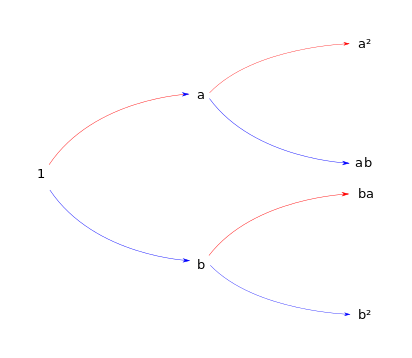
\includegraphics{images/groups_06_1.png}
\caption{Page1}
\end{figure}

%\DiaryEntry{Inside Interesting Integrals, Section 4.1 + 4.2 (Gamma and Beta Function)}{2016-03-30}{Integrals}

\subsection{Gamma Function}

The gamma function is defined as follows:

\[
\Gamma(n) = \int_0^\infty e^{-x} x^{n-1} dx, \quad n > 0
\]

We can use this to calculate the following integral

\[
\int_0^\infty \exp \left( -x^3 \right)dx
\]

by making the substitution \(y = x^3\): We have
\(\frac{dy}{dx} = 3x^2 \rightarrow dx = \frac{dy}{3x^2}\). We can
``reverse'' the substitution and obtain \(x = y^{1/3}\) and therefore
\(dx = \frac{dy}{3y^{2/3}} = \frac{1}{3}y^{-2/3} dy\). Inserting into
the integral yields

\[
\int_0^\infty \exp \left( -x^3 \right)dx = \int_0^\infty \exp(-y) \frac{1}{3}y^{-2/3} dy = \frac{1}{3} \Gamma \left( \frac{1}{3} \right) = \Gamma \left( \frac{4}{3} \right)
\]

where we used \(\Gamma(n+1) = n \Gamma(n)\) in the last step.

We can directly extend this to the more general case

\[
\int_0^\infty \exp \left( -x^n \right)dx, \quad n > 0
\]

We set \(y = x^n\),
\(\frac{dy}{dx} = n x ^{n-1} = n y^{\frac{n-1}{n}}\). Therefore
\(dx = \frac{dy}{n y^{\frac{n-1}{n}}} = \frac{1}{n} y^{\frac{1-n}{n}} dy\)
and we obtain

\[
\int_0^\infty \exp \left( -x^n \right) dx = \int_0^\infty \exp(-y) \frac{1}{n} y^{\frac{1-n}{n}} dy = \frac{1}{n} \Gamma \left( \frac{1}{n} \right) = \Gamma\left( \frac{n+1}{n} \right)
\]

We see that for \(n \rightarrow \infty\) the integral approaches 1.

The Figure below shows the function \(\exp \left( -x^n \right)\) for
values \(n=3\) (red), \(n=4\) (blue), and \(n=6\) (green).

\begin{figure}[H]
\centering
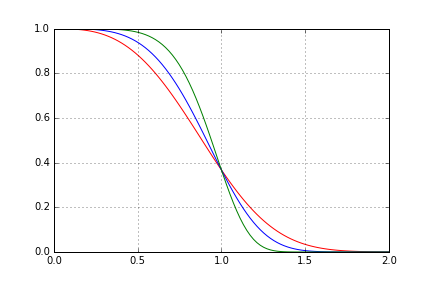
\includegraphics{images/interesting_integrals_05_1.png}
\end{figure}

Something else is interesting: We can substitute \(x=u^2\) in the
definition of the gamma function.
\(\frac{dx}{du}=2u \rightarrow dx=2u du\) and we obtain

\[
\Gamma(n) = \int_0^\infty e^{-x} x^{n-1} dx = \int_0^\infty e^{-u^2} u^{2(n-1)} 2u du = 2 \int_0^\infty e^{-u^2} u^{2n-1} du
\]

We can simplify the integral (and complicate the expression in the gamma
function); i.e.~we have

\[
\int_0^\infty e^{-u^2} u^m du = \frac{1}{2} \Gamma \left( \frac{m+1}{2} \right)
\]

This substitution trick can also be extended to integrands of the form
\(e^{-u^n} u^m\) - the definite integrals can then be expressed in terms
of the gamma function.

We make the substitution
\(u^n = x \rightarrow u=x^{1/n} \rightarrow u^m = x^{m/n}\) and we have
\(\frac{du}{dx} = \frac{1}{n}x^{1/n - 1}\). Using this, we obtain

\[
\int_0^\infty e^{-u^n} u^m du = \int_0^\infty e^{-x} x^{m/n} \frac{1}{n} x^{1/n-1} dx = \frac{1}{n} \int_0^\infty  e^{-x} x^{m/n + 1/n - 1} dx = \frac{1}{n} \Gamma \left( \frac{m+1}{n} \right)
\]

\subsection{Beta Function}

The Beta function is defined as

\[
B(m,n) = \int_0^1 x^{m-1} (1-x)^{n-1} dx, \quad m,n > 0
\]

From above we know that we can rewrite the Gamma function

\[
\Gamma(n) = 2 \int_0^\infty e^{-u^2} u^{2n-1} du
\]

Note that the integral does not depend on the name of the integration
variable; therefore we can write

\[
\Gamma(m) \Gamma(n) = 4 \int_0^\infty e^{-x^2} x^{2n-1} dx \int_0^\infty e^{-y^2} y^{2m-1} dy = 4 \int_0^\infty \int_0^\infty e^{-(x^2+y^2)} x^{2m-1} y^{2n-1} du
\]

We can express this integral in terms of polar coordinates;
\(r^2 = x^2 + y^2\) and \(dx dy = r dr d\phi\):

\[
\Gamma(m) \Gamma(n) = 4 \int_{r=0}^\infty \int_{\phi=0}^{\pi/2}  e^{-r^2} (r \cos \phi)^{2m-1} (r \sin \phi)^{2n-1} r dr d\phi
\]

which we can rewrite as follows

\[
\Gamma(m) \Gamma(n) = \left[ 2 \int_{r=0}^\infty e^{-r^2} r^{2(m+n)-1} dr \right] \left[  \int_{\phi=0}^{\pi/2}   (\cos \phi)^{2m-1} (\sin \phi)^{2n-1} d \phi \right]
\]

The first expression in brackets is simply \(\Gamma(m+n)\), for the
second expression we substitute \(x=\cos^2 \phi\) in the Beta function

\[
B(m,n) = \int_0^1 x^{m-1} (1-x)^{n-1} dx = -2 \int_{\pi/2}^0 (\cos \phi)^{2m-2} (\sin \phi)^{2n-2} sin\phi \cos\phi d\phi
\]

where we have used \(dx = -2 \sin \phi \cos \phi d \phi\) and
\(1 - x = \sin^2 \phi\). We can further simplify this as

\bee
B(m,n) = 2 \int_0^{\pi/2} (\cos \phi)^{2m-1} (\sin \phi)^{2n-1} d\phi
\eee

which is exactly the second expression above; and therefore we have

\[
\Gamma(m) \Gamma(n) = \Gamma(m+n) B(m,n)
\]

or

\bee
B(m,n) = \frac{\Gamma(m) \Gamma(n)}{\Gamma(m+n)}
\eee

\subsubsection{Plots}

The following Figure shows the integrand for various values of m and n:
Red corresponds to \(m=2, n=2\), blue corresponds to \(m=3, n=1\), green
corresponds to \(m=1, n=3\), and black corresponds to \(m=n=3\).

\begin{figure}[H]
\centering
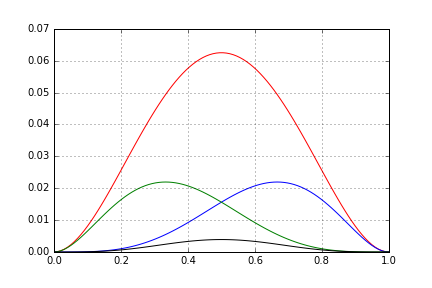
\includegraphics{images/interesting_integrals_05_2.png}

\end{figure}

The integrand is symmetric with respect to \(m,n\); therefore the Beta
function is symmetric in \(m,n\); i.e. \(B(m,n) = B(n,m)\).

The Figure below shows a contour plot of the Beta function.

\begin{figure}[H]
\centering
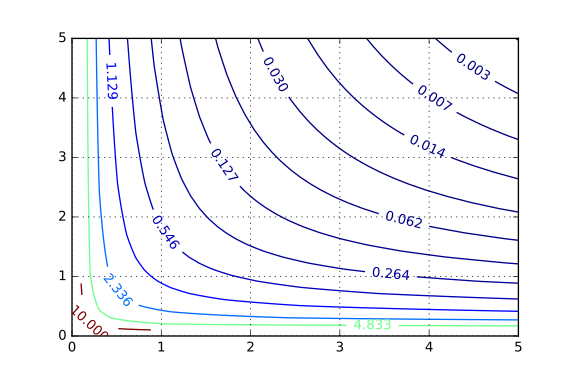
\includegraphics{images/interesting_integrals_05_3.png}
\end{figure}

\subsubsection{Properties}

The special values of \(B(m,1)\) and \(B(m,2)\) equal

\[
B(m,1) = \int_0^1 x^{m-1} (1-x)^0 dx = \left. \frac{x^m}{m} \right|_0^1 = \frac{1}{m}
\]

and

\[
B(m,2) = \int_0^1 x^{m-1} (1-x)^1 dx = \left. \frac{x^m}{m} - \frac{x^{m+1}}{m+1} \right|_0^1 = \frac{1}{m} - \frac{1}{m+1} = \frac{1}{m(m+1)}
\]

Calculating \(B(m,m)\) does not seem to be so easy; the first values are
\(B(1,1)=1, B(1,1)=1, B(2,2)=1/6, B(3,3)=1/30, B(4,4)=1/140, B(5,5)=1/630\).
I have no idea if there is a closed expression for this and what it is
(if it even exists). Neither does
\href{https://oeis.org/search?q=1\%2C6\%2C30\%2C140\%2C630\&language=german\&go=Suche}{OEIS}\ldots{}

We have \(B(m,n) = B(m,n+1) + B(m+1,n)\) by the following reasoning:

\begin{align*}
  B(m,n+1) + B(m+1,n) &= \int_0^1 x^{m-1} (1-x)^{n} dx + \int_0^1 x^{m} (1-x)^{n-1} dx \\
               &= \int_0^1 x^{m-1} (1-x)^{n-1} \left[(1-x) + x\right] dx = \int_0^1 x^{m-1} (1-x)^{n-1} dx = B(m,n)
\end{align*}

Another property is \(B(m,n) = \frac{m-1}{n} B(m-1, n+1)\) which we can
show by integration by parts ($v = x^{m-1}, u' = (1-x)^{n-1}$, and therefore $u = -(1-x)^n/n, v' = (m-1)x^{m-2}$):

\[
B(m,n) = \int_0^1 x^{m-1} (1-x)^{n-1} dx = \left. - \frac{1}{n} (1-x)^n x^{m-1} \right|_0^1 + \int_0^1 \frac{1}{n} (1-x)^n (m-1) x^{m-2} dx
\]

The first term becomes zero and the integral can be further expressed as

\[
B(m,n) = \frac{m-1}{n} \int_0^1 x^{m-2} (1-x)^n dx = \frac{m-1}{n} B(m-1, n+1)
\]

There are also \(B(m+1,n)= \frac{m}{m+n}B(m,n)\) and
\(B(m,n+1)=\frac{n}{m+n}B(m,n)\) which can be proven as follows:

\[
B(m+1,n) = \frac{\Gamma(m+1)\Gamma(n)}{\Gamma(m+n+1)} = \frac{m \Gamma(m)\Gamma(n)}{\Gamma(m+n)} = \frac{m}{m+1}B(m,n)
\]

where we have used \(\Gamma(m+1) = m \Gamma(m)\). The second identity
follows analogously.

Doing this a bit more extensively, we arrive at

\[
B(m+1,n+1) = \frac{mn}{(m+n+1)(m+n)}B(m,n)
\]

With the recursion start \(B(1,1) = 1\), we can recursively calculate
the values for the Beta function.

Using the substitution \(x = y/(1+y)\) we arrive at a different
definition of the Beta function. We have \(1 - x = 1/(1+y)\) and
differentiating both sides with respect to \(y\), we obtain

\[
-\frac{dx}{dy} = -\frac{1}{(1+y)^2} \rightarrow \frac{dx}{dy} = \frac{1}{(1+y)^2}
\]

With \(y = x/(1-x)\), the limits of the integral become
\(x=0 \rightarrow y=0\) and \(x=1 \rightarrow y=\infty\) and we finally
obtain

\begin{align*}
  B(m,n) &= \int_0^1 x^{m-1} (1-x)^{n-1} dx = \int_0^\infty \frac{y{m-1}}{(1+y){m-1}} \frac{1}{(1+y){n-1}} \frac{1}{(1+y)^2} dy\\
  &= \int_0^\infty \frac{y^{m-1}}{(1+y)^{m+n}} dy
\end{align*}

Using the binomial expansion \((1-x)^n = \sum_k {n \choose k} (-x)^k\)
we arrive at

\[
B(m,n) = \int_0^1 x^{m-1} \sum_k {n-1 \choose k} (-x)^k dx = \int_0^1 \sum_k {n-1 \choose k} x^{m-1} (-x)^k dx
\]

which is - well - probably somehow useful.

\subsubsection{Applications}

The integral

\[
\int_0^{\pi/2} \sqrt{\sin x} dx
\]

can be solved by making the substitution \(u=\sin^2 x\): We have
\(du/dx = 2 \sin x \cos x\) which can be expressed (using
\(\sin x= \sqrt{u}, \cos x = \sqrt{1-u}\)) as

\[
\int_0^1 u^{1/4} \frac{du}{2\sqrt{u}\sqrt{1-u}} = \frac{1}{2} \int_0^1 u^{1/4} u^{-1/2} (1-u)^{-1/2} du = \frac{1}{2} \int_0^1 u^{-1/4} (1-u)^{-1/2} du = \frac{1}{2} B(3/4,1/2)
\]


%%% Local Variables:
%%% mode: latex
%%% TeX-master: "journal"
%%% End:

%\DiaryEntry{Groups - Cyclic Subgroups of the Symmetric Group}{2016-04-12}{Algebra}


Consider two group elements \((), a = (1,2,3)\): 1 moves to 2, 2 to 3,
and 3 to 1. Repeating this operation, we arrive at \(a^2 = (1,3,2)\) and
finally \(a^3 = (1,2,3)\). That is, we have a cyclic group with elements
\(1, a, a^2\); i.e. \(a\) is the generator for this cyclic subgroup.

This is nice and can be extended; i.e.~a cycle \(a\) consisting of \(n\)
elements gives rise to a cyclic group of order \(n\) (with \(a\) being
the generator).

We can also consider permutations with 2 disjoint cycles; e.g.
\(a = (1,2,3),(4,5)\). The first cycle alone would create a subgroup of
order three (see above), the second cycle would create a subgroup of
order two (\((), (4,5)\) as \((4,5)^2 = ()\)). An element with these two
cycles is also a generator of a subgroup, however this subgroup has
order 6: \(a^2\) makes the second cycle become \(()\) as
\((4,5)^2 = ()\), however the first cycle would not become unity
(\((1,2,3)^2 \neq ()\)). On the other hand, \(a^3\) makes the first
cycle become unity (\((1,2,3)^3 = ()\)), but not the second one
(\((4,5)^3 \neq ()\)). Only \(a^6\) makes both cycles equal to unity,
therefore the resulting cyclic subgroup has order 6.

This can be generalized in that a permutation consisting of n disjoint
cycles \(a_1, \ldots a_n\) each with length \(l_1, \ldots, l_n\) is the
generator for a cyclic subgroup of order \(lcm(l_1, \ldots, l_n)\) where
lcm denotes the least common multiplier.

\subsection{Subbgroups of $S_3$}

This group has 6 elements. By the Laplace theorem, the (non-trivial)
subgroups must have 2 or 3 elements.

The 2-element subgroups are of the form \(()\) (the identity element)
and \((1,2)\). We have \((1,2) \star (1,2) = ()\); i.e. \((1,2)\) is its
own inverse. This is naturally the case as in a group with 2 elements (1
and a), we need to have \(a=a^{-1}\). The other 2-element subgroups are
\((), (1,3)\) and \((), (2,3)\).

A 3-element subgroup is \((), (1,2,3), (1,3,2)\). We have
\((1,2,3) \star (1,3,2) = ()\) and \((1,3,2) \star (1,2,3) = ()\) so we
have a subgroup.

The other 3-element subgroups are \((1,2,3)\) and \((2,1,3)\). These are
also cyclic subgroups; i.e.~the first group is
\((), (1,2,3), (1,2,3)^2, (1,2,3)^3 = ()\).

\subsection{\texorpdfstring{Subbgroups of
\(S_4\)}{Subbgroups of S\_4}}\label{subbgroups-of-s_4}

This group has 24 elements, therefore it must have subgroups of order
\(2,3,4,6,8,12\). It seems non-trivial to generate all these subgroups;
for an answer see
\href{https://math.stackexchange.com/questions/379841/how-to-enumerate-subgroups-of-each-order-of-s-4-by-hand?lq=1}{here}

%\DiaryEntry{Euclidian Distance Matrices}{2016-04-21}{maths}


This is based on \href{http://arxiv.org/pdf/1502.07541.pdf}{this paper},
located also \href{\%7Bfilename\%7D/files/1502.07541.pdf}{here}.

\subsubsection{Derivation of (3)}\label{derivation-of-3}

\begin{figure}[H]
\centering
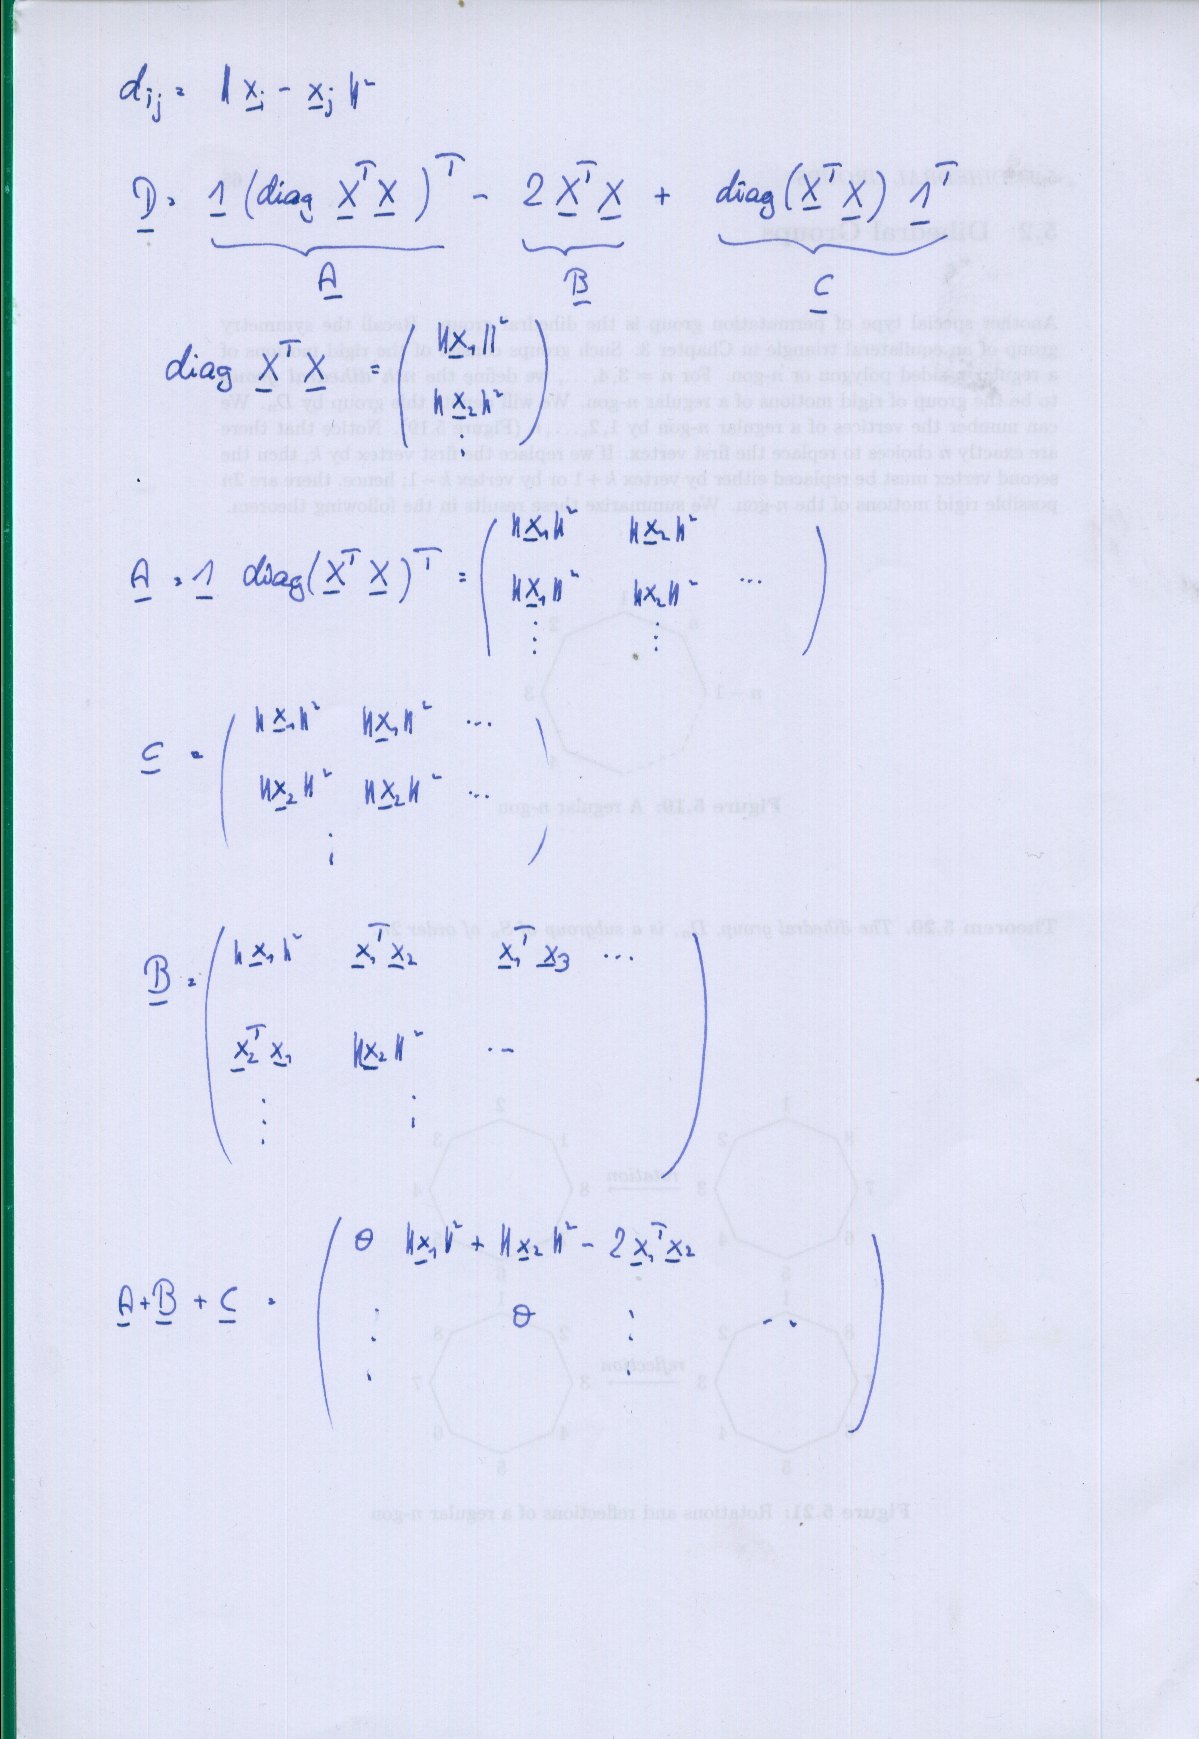
\includegraphics[scale=0.5]{images/edm_0001.png}
\end{figure}

\subsubsection{Derivation of II - B}\label{derivation-of-ii---b}

The n points in a d-dimensional Euclidean space are stored in the
columns of a matrix \(X = [x_1 x_2 \cdots x_n]\).

The edm of this matrix is given by


\begin{equation}
\label{edm_def}
edm(X) = \mathbf{1} \text{diag}(X^T X)^T - 2 X^T X + \text{diag}(X^T X) \mathbf{1}^T
\end{equation}


The task is to reconstruct the matrix X (the points) based on (an
estimate of) the euclidian distance matrix. Later Sections of the paper
deal with noisy and non-complete observations of the EDM but in the
beginning it is assumed that the EDM is fully and correctly known.

The first assumption (leading to (8) etc) is that \(x_1\) lies at the
origin. Then the first part of the EDM expression above becomes
\(\mathbf{1} \text{diag}(X^T X)^T = \mathbf{1} D e_1\) (with \(e_1\)
begin the first unit vector; i.e. \(e_1 = (1 0 \cdots 0)^T\) and
therefore \(D e_1\) selects the first column of D).

Therefore, we can solve the equation above for \(X^T X\) as follows:

\[
X^T X = -\frac{1}{2} \left[ edm(X) - \mathbf{1} d_1^T - d_1 \mathbf{1}^T \right]
\]

We can obtain from \(X^T X\) the matrix \(X\) by performing an
eigenvalue decomposition \(X^T X = U \Lambda U^T\). Then
\(X_{\text{sqrt}} = \sqrt{\Lambda} U^T\) and
\(X_{\text{sqrt}}^T X_{\text{sqrt}} = X^T X\).

Assuming that the eigenvalues are ordered by size, we throw away all but
the first n ones. The esimtated matrix \(X_{\text{est}}\) is then given
by \(X_{\text{est}} = \sqrt{\Lambda} U^T\).

\subsubsection{Uniqueness of EDM}\label{uniqueness-of-edm}

If we rotate and/or shift the point matrix \(X\), the edm should stay
the same. A rotaion is expressed as \(\tilde{X} = QX\), where \(Q\) is
an orthogonal matrix; i.e. \(Q^T Q = I\). In the EDM expression
\(\eqref{edm_def}\), only the term \(X^T X\) appears; considering
\(\tilde{X}\) instead, we have
\(\tilde{X}^T \tilde{X} = X^T Q^T Q X = X^T X\) - a rotation does not
affect the EDM.

In a similar spirit, we can show that a linear translation
\(X_t = X + b 1^T\) leaves the emd intact; i.e. \(edm(X_t) = edm(X)\).

%\DiaryEntry{Sum of Gaussian RVs, Characteristic Functions}{2016-04-22}{Stochastic}


We can calculate the pdf of the sum of two Gaussian RVs also by means of
characteristic functions. The characteristic function of a pdf is
defined as its fourier transform; therefore a convolution of two pdfs
(which we need to perform to obtain the sum pdf) corresponds to the
multiplication of their characteristic functions.

\subsection{Characteristic Function}

We have for the pdf

\[
f_X(x) = \frac{1}{\sqrt{2\pi \sigma^2}} \exp \left( - \frac{(x-\mu)^2}{2\sigma^2} \right)
\]

and the characteristic function becomes

\[
\phi_X(t) = \int_{- \infty}^\infty f_X(x) \exp (jtx) dx = c \int_{- \infty}^\infty \exp \left( - \frac{(x-\mu)^2}{2\sigma^2} + jtx \right) dx
\]

We continue and obtain

\[
\phi_X(t) = c \int_{- \infty}^\infty \exp \left(- \frac{ x^2 - 2x\mu + \mu^2 - jtx2\sigma^2 }{2\sigma^2} \right) dx
\]

There will be a lot of terms and it is important to realize that
everything which does not depend on \(x\) or \(t\) can be moved in front
of the integral and ignored. Therefore, we arrive at

\[
\phi_X(t) = c' \int_{- \infty}^\infty \exp \left( - \frac{ x^2 - 2x\mu - jtx2\sigma^2 }{2\sigma^2} \right) dx
\]

and continue considering the nominator of the exponent alone:

\[
x^2 - 2x\mu - jtx2\sigma^2 = x^2 - 2x(\mu + jt\sigma^2) = \left( x-(\mu + jt\sigma^2) \right)^2 - (\mu + jt\sigma^2)^2
\]

where we have competed the square in the last expression. Now, we can
put that back into our integral expression and obtain

\[
\phi_X(t) = c' \exp \left(\frac{ (\mu + jt\sigma^2)^2 }{2\sigma^2} \right)  \int_{- \infty}^\infty \exp \left(- \frac{ \left( x-(\mu + jt\sigma^2) \right)^2 }{2\sigma^2} \right) dx
\]

We see that the integral is of the form
\(\int_{- \infty}^\infty \exp (x-A)^2dx\) and this is a constant
independent of \(x\) \textbf{and} \(t\) (It will depend on \(\sigma^2\),
however). Therefore, the only expression depending on \(t\) is the one
before the integral and this can be simplified to (by leaving out
constant terms again)

\[
\phi_X(t) = \exp \left( j\mu t - \frac{\sigma^2 t^2}{2}\right)
\]

\subsection{Sum of RVs}

Not things become simple. We have two Gaussian Rvs \(X_1, X_2\) with
distributions \(f_1(x) = \mathcal{N}(x, \mu_1, \sigma_1^2)\) and
\(f_2(x) = \mathcal{N}(x, \mu_2, \sigma_2^2)\), respectively.

The characteristic function of their sum \(X\) is the product of their
characteristic functions; i.e.

\[
\phi_X(t) = \exp \left( j\mu_1 t - \frac{\sigma_1^2 t^2}{2}\right) \exp \left( j\mu_2 t - \frac{\sigma_2^2 t^2}{2}\right) = \exp \left( j(\mu_1 + \mu_2) t - \frac{(\sigma_1^2 + \sigma_2^2) t^2}{2}\right)
\]

and this is the characteristic function of a Gaussian RV with
distribution
\(f(x) = \mathcal{N}(x, \mu_1 + \mu_2, \sigma_1^2 + \sigma_2^2)\).

%\DiaryEntry{Integration - Symmetries}{2016-04-25}{Integrals}

We have a continuous function \(f\) which is even on the interval
\([-a, a]\) (\(a>0\)).

The integral

\[
I = \int_{-a}^a \frac{f(x)}{1 + e^x} dx
\]

can be simplified as follows. First, we can rewrite the integral as

\[
I = \int_{-a}^a \frac{f(x)}{1 + e^{-x}} dx
\]

by substituting \(x \rightarrow -x\) and using the fact that \(f(x)\) is
even (\(f(x) = f(-x)\) on the integration interval). Then we have

\[
2I = \int_{-a}^a \frac{f(x)}{1 + e^x} dx + \int_{-a}^a \frac{f(x)}{1 + e^{-x}} dx = \int_{-a}^a f(x) \left( \frac{1}{1 + e^x} + \frac{1}{1 + e^{-x}} \right) dx
\]

which simplifies to

\[
2I =  \int_{-a}^a f(x) dx = 2 \int_{0}^a f(x) dx
\]

again using the evenness of \(f(x)\). This means that we have

\[
\int_{-a}^a \frac{f(x)}{1 + e^x} dx = \int_{0}^a f(x) dx
\]

\subsubsection{Example}

Consider the following integral

\[
I = \int_{-\pi/2}^{\pi/2} \frac{\cos x}{1+e^{x}} dx
\]

The function \(\cos x\) is even, therefore we can use the trick
mentioned above. Therefore, we have

\[
I = \int_0^{\pi/2} \cos x dx = \sin x \Big|_0^{\pi/2} = 1
\]

The Figure below shows the plot of the two integrands: red = original
expression, blue = simplified expression. Note that the integration
interval of the simplified expression is half the interval of the
complicated expression.

It is interesting to note that such a complicated expression and plot
can be simplified to such a great extent. On the other hand, it is
\textbf{just} the value of the integral which stays constant - it is
less surprising that two functions which look differently yield the same
integral value.

\begin{figure}
\centering
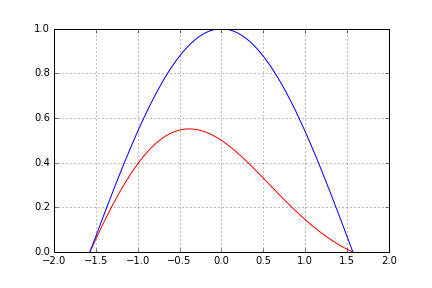
\includegraphics{images/integration-symmetries.png}
\end{figure}

%\DiaryEntry{Groups - Isomorphisms}{2016-04-27}{Algebra}


Two groups G and H are isomorphic, if there exists a one-to-one and onto
map $\phi:G \rightarrow H$ such that the group operation is preserved;
i.e.

\[
\phi(a \star b) = \phi(a) \star \phi(b)
\]

for all \(a,b \in G\). If G is isomorphic to H, we write \(G \cong H\).
The map $\phi$ is called an isomorphism.

A necessary, but not sufficient condition for two groups to be
isomorphoc is that they have the same number of elements. However, this
is ot sufficient - the group structure and the isomorphism \(\phi\) must
also match.

As example consider the symmetric group \(S_3\) and \(\mathbb{Z}_6\)
which have the same number of elements but are not isomorphic because
\(\mathbb{Z}_6\) is abelian whereas \(S_3\) is not. Assume
\(\phi: \mathbb{Z}_6 \rightarrow S_3\) is an isomorphism and choose two
elements \(a,b \in S_3\) for which \(a \star b \neq b \star a\). Since
\(\phi\) is an isomorphism, there exist \(m,n \in \mathbb{Z}_6\), such
that \(\phi(m) = a, \phi(n) = b\). However,
\(ab = \phi(m)\phi(n) = \phi(m+n) = \phi(n+m) = \phi(n) \phi(m) = b a\)
which contradicts the assumption that \(a,b\) do not commute.

\subsubsection{Example}\label{example}

We want to show that \(\mathbb{Z}_4\) is isomorphic to the cyclic group
\(\langle j \rangle\) under the map \(\phi(n) = j^n\).

We have \(\phi(0) = 1, \phi(1) = j, \phi(2) = -1, \phi(3) = -i\).
Therefore, the map is one-to-one and onto and we have
\(\phi(m+n) = i^{m+n} = \phi(m) \phi(n)\).

\subsection{Properties}\label{properties}

If \(\phi : G \rightarrow H\) is an isomorphism of two groups. Then the
following statements are true:

\begin{itemize}
\item
  \(\phi^{-1} : H \rightarrow G\) is also an isomorphism.
\item
  \(|G| = |H|\)
\item
  If G is abelian, then H is also abelian.
\item
  If G is cyclic, then H is also cyclic.
\item
  If G has a subgroup of order n, then H has a subgroup of order n
\end{itemize}

Furthermore, we can characterize all cyclic groups:

\begin{itemize}
\item
  All cyclic groups of infinite order are isomorphic to \(\mathbb{Z}\).
\item
  If G is a cyclic group of order n, then G is isomorphic to
  \(\mathbb{Z}_n\).
\end{itemize}

\subsection{Cayley's Theorem}\label{cayleys-theorem}

Cayley's Theorem states that every group is isomorphic to a group of
permutations (i.e.~a subgroup of the symmetric group).

\subsubsection{Example}\label{example-1}

Consider the group \(\mathbb{Z}_3\) with table

\[
\begin{array}{c|ccc}
\star & 0 & 1 & 2 \\ \hline
0       & 0 & 1 & 2 \\
1       & 1 & 2 & 0 \\
2       & 2 & 0 & 1
\end{array}
\]

and a permutation group \(G = \{(), (0,1,2), (0,2,1)\}\). If we perform
the following mapping

\[
\begin{array}{cc}
0 \leftrightarrow & ()  \\
1 \leftrightarrow & (0,1,2)  \\
2 \leftrightarrow & (0,2,1)  \\
\end{array}
\]

then we have an isomorphism between \(\mathbb{Z}_3\) and G. E.g.
\((0,1,2) \star (0,2,1) = ()\) which corresponds to \(1 \star 2 = 0\).

\subsubsection{Also interesting}\label{also-interesting}

The symmetric group \(S_n\) has \(n!\) members. By the Lagrange theorem,
it has subgroups which order divides \(n!\) and this is \textbf{every
integer} from 1 to n (\(n! = 2 \times 3 \times \cdots n\)). This is a
strong indication that \(S_n\) has subgroups of order \(1,2,\ldots,n\).

\subsubsection{Proof}\label{proof}

Given a group \(G\), we need to find a group of permutations \(\bar{G}\)
that is isomorphic to \(G\).

\paragraph{Horribly complicated - I don't get it
:-(}\label{horribly-complicated---i-dont-get-it--}

For any \(g \in G\), define a function \(\lambda_g : G \rightarrow G\)
by \(\lambda_g(a) = ga\).

We claim that \(\lambda_g\) is a permutation of \(G\). To show that
\(\lambda_g\) is one-to-one, suppose that
\(\lambda_g(a) = \lambda_g(b)\). Then
\(ga =\lambda_g(a) = \lambda_g(b) = gb\). Hence, \(a = b\). To show that
\(\lambda_g\) is onto, we must prove that for each \(a \in G\), there is
a \(b\) such that \(\lambda_g (b) = a\). Let \(b = g^{-1} a\).

Now we are ready to define our group \(\overline{G}\). Let
\(\overline{G} = \{ \lambda_g : g \in G \}\). We must show that
\(\overline{G}\) is a group under composition of functions and find an
isomorphism between \(G\) and \(\overline{G}\). We have closure under
composition of functions since
\((\lambda_g \circ \lambda_h)(a) = \lambda_g(ha) = gha = \lambda_{gh}(a)\).
Also, \(\lambda_e (a) = ea = a\) and
\((\lambda_{g^{-1}} \circ \lambda_g) (a) = \lambda_{g^{-1}} (ga) = g^{-1} g a = a = \lambda_e(a)\).

We can define an isomorphism from \(G\) to \(\overline{G}\) by
\(\phi : g \mapsto \lambda_g\). The group operation is preserved since
\(\phi(gh) = \lambda_{gh} = \lambda_g \lambda_h = \phi(g) \phi(h)\). It
is also one-to-one, because if \(\phi(g)(a) = \phi(h)(a)\), then
\(ga = \lambda_g a = \lambda_h a= ha\). Hence, \(g = h\). That \(\phi\)
is onto follows from the fact that \(\phi( g ) = \lambda_g\) for any
\(\lambda_g \in \overline{G}\)

%\DiaryEntry{Groups - External Direct Product}{2016-04-29}{Algebra}


If we have two groups \((G, \star)\) and \((H, \circ)\) then we can make
the Cartesian product of G and H into a new group. The new group is just
the ordered pairs \((g, h) \in G \times H\) and we define a binary
operation on \(G \times H\) by
\((g_1, h_1)(g_2, h_2) = (g_1 \star g_2, h_1 \circ h_2)\) - i.e.~we
multiply elements in the first coordinate as we do in G and and elements
in the second coordinate as we do in H.

The result of this is a group, as

\begin{itemize}
\item
  the binary operation is closed.
\item
  If \(e_G\) and \(e_H\) are the identities of the groups G and H
  respectively, then \((e_G, e_H)\) is the identity of \(G \times H\).
\item
  The inverse of \((g, h) \in G\times H\) is \((g^{-1}, h^{-1})\).
\end{itemize}

\subsubsection{Example}\label{example}

Let \(\mathbb{R}\) be the group of real numbers under addition. The
Cartesian product of \(\mathbb{R} \times \mathbb{R}\) is also a group,
in which the group operation is just addition in each coordinate; that
is, \((a, b) + (c, d) = (a + c, b + d)\). The identity is (0,0) and the
inverse of \((a, b)\) is \((-a, -b)\).

The external product can be extended to the Cartesian product of \(M\)
groups; for example \(\mathbb{Z}_2^M\) is a group of all binary
M-tuples. The group operation is the \emph{exclusive or} of two binary
M-tuples.

\subsection{Internal Direct Product}\label{internal-direct-product}

The external product makes a larger group out of two (or more) smaller
groups. The internal direct product allows to express a large group as
isomorphic to the direct product of two of its subgroups.

Let G be a group with subgroups H and K satisfying the following
conditions:

\begin{itemize}
\item
  G can be expressed by combining elements of the two subgroups by the
  group operation; i.e. \(G = HK = \{ h \star k : h \in H, k \in K \}\).
\item
  \(H \cap K = \{ e \}\)
\item
  \(hk = kh\) for all \(k \in K\) and \(h \in H\)
\end{itemize}

Then G is the \emph{internal direct product} H and K. The above three
conditions are pretty strong in the sense that it is rather easy to find
subgroups of a given group; however finding two subgroups from which the
original group can be constructed is much harder. I would assume that
only few groups can be expressed as internal direct prduct.

As an example consider the group of unity \(U(8) = \{1,3,5,7\}\). If we
define two subgroups \(H = \{1,3\}\) and \(K = \{1,5\}\), we can express
G as product of the elemts of the subgroups (the only non-obvious case
is \(3 \star 5 = 3 \times 5 \mod 8 = 7\)). The subgroups H and K do not
share any element apart the unit element and finally \(U(8)\) is an
Abelian group. Therefore \(U(8)\) is the internal direct product of H
and K.

Another example is \(G = \mathbb{Z}_4\) with modulo-4 addition. If we
define \(H=\{0,2\}\) and \(K=\{0,1\}\), then we express every element of
\(G\) by combining elements from H and K, and H and K do not share any
element apart from the identity element. Since G is abelian, the last
condition is fulfilled as well.

%\DiaryEntry{Normal Subgroups}{2016-05-10}{Algebra}

A subgroup H of a group G is normal in G if \(gH = Hg\) for all
\(g \in G\). That is, a normal subgroup of a group G is one in which the
right and left cosets are precisely the same.

Let G be a group and N be a subgroup of G. Then the following statements
are equivalent:

\begin{itemize}

\item
  The subgroup N is normal in G.
\item
  For all \(g \in G\) , \(gNg^{-1}\) is a subset of N.
\item
  For all \(g \in G\) , \(gNg^{-1}\) actually is N.
\end{itemize}

If the group G is abelian, then every subgroup of G is a normal
subgroup. This is easy and a strong condition on the group G. More
interesting are non-abelian groups which nevertheless have normal
subgroups. Existence will depend on the group G itself, but also on the
subgroup (i.e.~not all subgroups H of a non-abelian group G are normal).

\subsection{Example}\label{example}

Consider the group \(\mathbb{Z}_6\) with group operation modulo-6
addition and a subgroup \(N=\{0,3\}\).

We need to check that the third condition from above holds.

\begin{itemize}
\item
  For \(g=0\), we have \(g^{-1}=0\) and (i)
  \(g 0 g^{-1}=0 \star 0 \star 0=0\) and (ii)
  \(g 3 g^{-1}=0 \star 3 \star 0 = 3\).
\item
  For \(g=1\), we have \(g^{-1}=5\) and (i)
  \(g 0 g^{-1}=1 \star 0 \star 5=0\) and (ii)
  \(g 3 g^{-1}=1 \star 3 \star 5 = 3\).
\item
  For \(g=2\), we have \(g^{-1}=4\) and (i)
  \(g 0 g^{-1}=2 \star 0 \star 4=0\) and (ii)
  \(g 3 g^{-1}=2 \star 3 \star 4 = 3\).
\item
  For \(g=3\), we have \(g^{-1}=3\) and (i)
  \(g 0 g^{-1}=3 \star 0 \star 3=0\) and (ii)
  \(g 3 g^{-1}=3 \star 3 \star 3 = 3\).
\item
  For \(g=4\), we have \(g^{-1}=2\) and everything is the same as for
  \(g=2\).
\item
  For \(g=5\), we have \(g^{-1}=1\) and everything is the same as for
  \(g=1\).
\end{itemize}

\subsection{Coset Multiplication}\label{coset-multiplication}

If H is a subgroup of G, then we can define coset multiplication as
\(Ha Hb = H(ab)\). This definition looks very simple, but it is not
clear, whether the product of two cosets defined in this way, is
uniquely defined. E.g. Ha may be the same coset a Hc (this happens when
\(c \in Ha\) and in a similar spirit, Hd may be the same coset as Hb.
Therefore, the product Ha Hb is the same as Hc Hd; however, the coset
H(ab) may not be the same coset as H(cd).

\subsection{Normal Subgroups, Coset Multiplication, and Quotient/Factor
Groups}\label{normal-subgroups-coset-multiplication-and-quotientfactor-groups}

If N is a normal subgroup of G, and if Ha=Hc and Hb=Hd, then
H(ab)=H(cd).

If Ha=Hc, then \(a \in Hc\) and \(a=h_1c\), and similar \(b=h_2d\). The
product \(ab\) then becomes \(ab = h_1 c h_2 d = h_1 (c h_2) d\). But
the left cosets equal the right ones and so we have \(c h_2 = h_3 c\)
and we can rewrite \(ab = h_1 h_3 c d = (h_1 h_3)(c d)\) and this
element is in H(cd). Since \(ab \in H(cd)\), we can deduce that
\(H(ab) = H(cd)\).

The set G/H is the set of all cosets of the subgroup H; i.e.
\(G/H=\{Ha, Hb, Hc, \ldots\}\) and this set forms a group under coset
multiplication:

\begin{itemize}
\item
  The identity element is \(H=He\), as \(Ha He = H(ae) = Ha\).
\item
  The inverse of \(Ha\) is H(a\^{}\{-1\})\$ because
  \(Ha Ha^{-1} = H(a a^{-1}) = He\).
\end{itemize}

Finally, \(G/H\) is a homomorphic image of G. We can choose
\(\phi(x) = Hx\) and this is a homomorphism because
\(\phi(xy) = H(xy) = Hx Hy = \phi(x) \phi(y)\).

\subsubsection{Example}\label{example-1}

Consider \href{\%7Bfilename\%7D2016-03-25-groups_05.markdown}{again} the
group \(\mathbb{Z}_6\) with group operation modulo-6 addition and a
subgroup \(N=\{0,3\}\). The cosets are


\begin{align*}
0 + H = 3 + H &= \{0,3\} \\
1 + H = 4 + H = &= \{1,4\} \\
2 + H = 5 + H &= \{2,5\} \\
\end{align*}


The theorem says that the three items \(0 + H\), \(1 + H\), and
\(2 + H\) form a group. The group operation is
\((a + H) \star (b + H) = (a \star b) + H\).

As an example, \((1+H) \star (0+H) = (1+H)\). The coset \(1+H\) contains
the elements \(\{1,4\}\), the coset \(0+H\) the elements \(\{0,3\}\). If
we combine the element from each coset by means of the group operation,
we obtain \(1+0=1, 1+3=4, 4+0=4, 4+3=1\) and this equals the coset
\(1+H\) as stated.

In a similar spirit, we have \((1+H)\star(2+H)=3+H=0+H\). Combining
elements from \(\{1,4\}\) and \(\{2,5\}\), we obtain
\(1+2=3, 1+5=0, 4+2=0, 4+5=3\) which equals the coset \(0+H\).

Continuing in this spirit, we obtain the operation table as follows:

\[
\begin{array}{c|ccc}
\star & 0+H & 1+H & 2+H \\ \hline
0+H   & 0+H & 1+H & 2+H \\
1+H   & 1+H & 2+H & 0+H \\
2+H   & 2+H & 0+H & 1+H
\end{array}
\]

\subsubsection{Interpretation}\label{interpretation}

In a way, a factor group is a reduction of group elements. Instead of
working with the group elements of N, we consider the cosets of N
instead. The cosets have a ``representative'' and a subgroup. The
``representative'' is the amount the subgroup is shifted by; e.g.~the
coset \(1 + H\) has 1 as ``representative'' and \(H\) is the subgroup -
in other words, the subgroup \(H\) is shifted by 1.

A factor group contains only the ``representative''. If the subgroup
(the cosets are based on) is normal, then the representatives themselves
form a group. The Figure below shows an example of a normal subgroup:
All a-arrows leaving H arrive at the left coset aH; and all arrows
arriving at aH come from the subgroup H. It is this property which
allows to drop the actual elements of the subgroup and consider the
coset ``representative'' instead.

\begin{figure}[H]
\centering
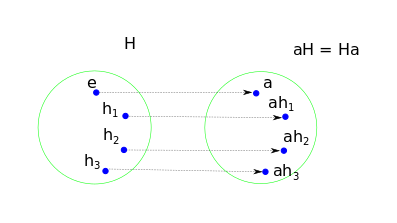
\includegraphics[scale=0.7]{images/groups_10_1.png}
\caption{Page1}
\end{figure}

%\DiaryEntry{Dice Problems, I}{2016-05-11}{Stochastic}

This is based on problems 1, 2, and 3
\href{http://www.madandmoonly.com/doctormatt/mathematics/dice1.pdf}{here};
locally stored \href{\%7Bfilename\%7D/files/dice1.pdf}{here}.

\subsection{Problem 1; Roll until a 6 comes up}

On average, how many times must a 6-sided die be rolled until a 6 turns
up?

One way of answering this question is to observe that the distribution
of throwing a 6 follows a
\href{\%7Bfilename\%7D2015-08-18-Geometric_Distribution.markdown}{Geometric
Distribution} and use the expectation of the distribution.

Another way, which is followed in the linked document, is to directly
set up an equation for the expectation E. When rolling a die for the
first time, there is a chance of 1/6 of rolling a 6. In this case, we
are done and the expected value \(E=1\). In all other cases (we throw
1\ldots{}5) with probability 5/6, we need to continue with another dice
throw. In other words, we start all over again. In this case, the
expected value is \(E+1\) (whatever value E is).

So we have

\[
E = \frac{1}{6} \times 1 + \frac{5}{6} \times (E+1)
\]

from which follows \(E=6\).

\subsection{Problem 2, Sequence of two sixes}

On average, how many times must a 6-sided die be rolled until a 6 turns
up twice in a row?

The expected number of rolls to come up with the first 6 is 6 (see
above). Once we have rolled a first 6, there are two options: (i) We
roll another 6 (with probability 1/6) and are done; (ii) we roll
something else (with probability 5/6) and need to start all over again.
In this case, the expected value is \(E+1\).

Therefore, we have

\[
E = 6 + \frac{1}{6} \times 1 + \frac{5}{6} \times (E+1)
\]

from which follows \(E=42\).

\subsection{Problem 3, Sequence of six and five}

On average, how many times must a 6-sided die be rolled until the
sequence 65 appears (i.e., a 6 followed by a 5)?

This one is a bit tricky / unintuitive.

We can express this with two equations and two expectations: Let \(E\)
denote the expected number of rolls till we have a 6-5; let \(E_6\) the
expected number of rolls till we have a 6-5, \textbf{after} having
thrown a 6.

For expressing \(E_6\), we note that we have \textbf{three} options
after we roll a 6: (i) we roll a 5 and are finished, (ii) we roll a 6
(and need to wait for a wait for a subsequent 5), (iii) we roll
something else (1\ldots{}4) and start all over again.

Therefore,

\[
E_6 = \frac{1}{6} \times 1 + \frac{1}{6} \times (E_6 + 1) + \frac{4}{6} (E+1)
\]

For expressing \(E\), we note that there are two options: (i) After we
have rolled a 6, we roll a 5 and are finished. This happens with
probability 1/6; (ii) in all othe cases, we need to start all over again
and the expected value is \(E+1\).

Therefore,

\[
E = \frac{1}{6} \times (E_6 + 1) + \frac{5}{6} \times (E+1)
\]

From these two equations we obtain \(E = 36\). Interestingly, this is
smaller than the expected number of throws till two consecutive sixes
come up.

\subsubsection{Further Thoughts}

The probability for length-2 sequences is independent how they are
stopped (5-6 or 6-6). In all cases, there are 36 possibilities (1-1, 1-2
\ldots{} 6-6) and one of them (either 5-6 or 6-6) stops. Therefore, the
probabilities for a length-2 sequence is \(1/36\).

The probabilitiy for length-3 sequences is similar. For stopping with
5-6, the first element must be from the set \(\{1,2,3,4,6\}\) and will
appear with probability \(5/6\). The 5-6 happens with probability
\(1/36\) and in total we are at \(5/216\). The same holds true for
stopping on a 6-6; the first element must be from the set
\(\{1,2,3,4,5\}\); but all probabilities are the same.

The probability for length-4 sequences are more involved. Let's start
with a stop sequence 5-6 first. We simply write down all length-4
combinations with the last 2 elements being 5-6.

\bee
\begin{array}{cc}
& 1 1 5 6 \\
& 1 2 5 6 \\
& \cdots \\
& 1 6 5 6 \\
& \cdots \\
& 5 5 5 6 \\
& \color{red}{5 6 5 6} \\
& 6 1 5 6 \\
& \cdots \\
& 6 6 5 6
\end{array}
\eee

The sequence in red is \textbf{not allowed} as it is actually a length-2
sequence. That means, we have \(35\) ``good'' cases out of \(6^4\) and
the probability of a length-4 sequence with stop sequence 5-6 is
\(35 / 6^4\).

If we have a stop sequence of 6-6, more sequences are not allowed; in
the block starting with 1, the sequence 1-6-6-6 is not allowed. This
holds for every block (i.e.~2-6-6-6, 3-6-6-6, 4-6-6-6, 5-6-6-6, and
6-6-6-6); therefore only 30 sequences remain and the probability of a
length-4 sequence with stop sequence 6-6 is \(30 / 6^4\).

This is somewhat counterintuitive; at first sight, sequences should have
the same probability irrespective of the stop sequence. However, with
some stop sequences, there are more ways that a sequence stops earlier;
these do not contribute to the good cases and therefore the probability
is less.

I am sure there is some expression for sequences with arbitrary lengths
and different stop sequences\ldots{}

%\DiaryEntry{Interesting Sums, III}{2016-05-21}{Maths}

\subsection{Sums with a factorial}

The exponential function \(\exp(x)\) has the following Taylor series
expansion:

\[
\exp(x) = \sum_{n=0}^\infty \frac{x^n}{n!}
\]

Taking derivatives with respect to \(x\) on both sides yields

\[
\exp(x) = \sum_{n=1}^\infty \frac{n x^{n-1}}{n!} = \sum_{n=1}^\infty \frac{x^{n-1}}{(n-1)!} = \sum_{n=0}^\infty \frac{x^n}{n!}
\]

Ok, this is not so interesting (especially as the LHS stays the same).

Let's try this

\[
\sum_{n=0}^\infty \frac{x^{n+1}}{n!} = \sum x \frac{x^n}{n!} = x \sum \frac{x^n}{n!} = x e^x
\]

Taking the derivative with respect to \(x\) yields

\[
e^x (1+x) = \sum_{n=0}^\infty \frac{(n+1)x^n}{n!}
\]

Considering \(x=1\), we obtain

\[
\sum_{n=0}^\infty \frac{(n+1)}{n!} = 2e
\]

We can differentiate another time and get

\[
e^x (2+x) = \sum_{n=0}^\infty \frac{n(n+1)x^{n-1}}{n!}
\]

which evaluates to

\[
\sum_{n=0}^\infty \frac{n(n+1)}{n!} = 3e
\]

at \(x=1\). Ladies and Gentlemen, I think we have a pattern here :-).
Start with

\[
\frac{d}{dx}xe^x = xe^x + e^x
\]

and

\[
\frac{d^2}{dx^2}xe^x = xe^x + e^x + e^x = xe^x + 2e^x
\]

and in general

\[
\frac{d^n}{dx^n}x e^x = xe^x + ne^x
\]

Evaluating this at \(x=1\) yields

\[
\left. \frac{d^n}{dx^n}x e^x \right|_{x=1} = (n+1)e
\]

and from this we obtain the sum

\[
\sum_{n} \frac{(n+1)^{\underline{m}}}{n!} = (m+1)e
\]

where \(x^{\underline{n}} = x(x-1)\cdots(x-n+1)\) is the falling
factorial.

%\DiaryEntry{Tilings}{2016-06-08}{Maths}

Consider a sequence \(l_n = 4n-3\). The first elements are
\(l_1=1, l_2=5, l_3=9, l_4=13,\ldots\). We are interested in the partial
sum

\[
S_N = \sum_{n=1}^N l_n
\]

An interpretation of the \(l_n\)s is shown in the Figure below: The
\(l_n\)s correspond to the number of squares in the same color: \(l_1\)
corresponds to the black square, \(l_2\) corresponds to the green
squares, \(l_3\) corresponds to the red squares, and \(l_4\) corresponds
to the blue squares.

\begin{figure}[H]
\centering
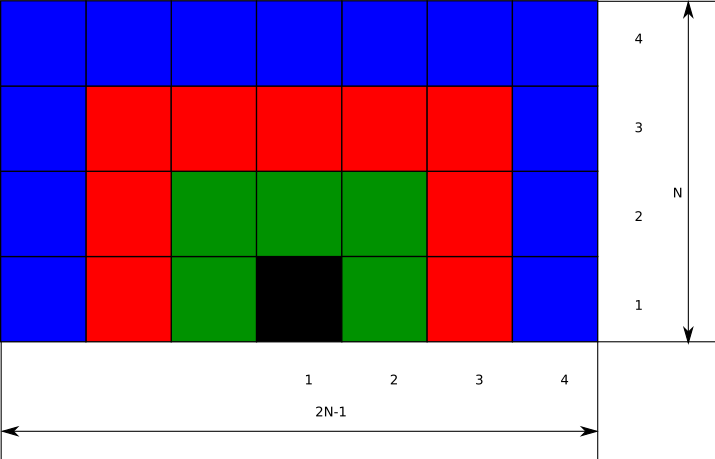
\includegraphics[scale=0.5]{images/tilings_01.png}
\end{figure}

The partial sum \(S_N\) is then the total number of squares contained in
a rectangle of width \(2N-1\) and height \(N\); therefore

\[
S_N = (2N-1)N
\]

and we deduce the following identity

\[
\sum_{n=1}^N 4n-3 = (2N-1)N
\]

%\DiaryEntry{Groups - Homomorphisms}{2016-06-13}{Algebra}

A homomorphism is defined as a mapping \(\phi\) from a group G to a
group H with the condition that

\[
\phi(a \star b) = \phi(a) \star \phi(b), \quad a,b \in G
\]

H is called the homomorphic image of G under \(\phi\).

The mapping need not (and typically will not) be one-to-one; in the
one-to-one case we would have an isomorphism.

The homomorphism has two properties:

\begin{itemize}
\item
  \(\phi(e) = e\). The homomorphic image of G's identity element is H's
  identity element. We can prove this by noting the general property
  that if \(y = e\), we have \(yy = ye = y\). Using this on
  \(\phi(e)\phi(e) = \phi(ee) = \phi(e) = e\) we deduce \(\phi(e) = e\).
\item
  \(\phi(a^{-1}) = [\phi(e)]^{-1}\). We can prove this by noting that
  \(\phi(e) \phi(e^{-1}) = \phi(e e^{-1}) = \phi(e) = e\). This means
  that \(\phi(e) \times A = e\) from which we deduce that A equals the
  inverse of \(\phi(e)\), namely \([phi(e)]^{-1}\).
\end{itemize}

\subsection{Normal Subgroups}\label{normal-subgroups}

There are two equivalent definitions for normal subgroups H of a group
G: (i) Left- and right cosets are equal; i.e. \(Ha = aH, a \in G\) and
(ii) \(xax^{-1} \in H, a \in H, x \in G\).

That these two definitions are equivalent can be seen as follows: If
\(y \in xH\) (\(x \in G\)), we can write \(y = xh\) for some
\(h \in H\). We can rewrite this as \(y = xhx^{-1}x\) where we have
``reingeschummelt'' an \(x\). Making things more explicit, we can write
\(y = (xhx^{-1})x\) and we know that $xhx^{-1} \in H$, so \(y = h'x\)
(with \(h' \in H\). But from cosets, we know that when two cosets share
the same element, they are actually equal and therefore, we have
\(Ha = Ha\).

Define the kernel of a homomorphism as all elements which get mapped to
the identity element by the homomorphism: $k(\phi) = \{x, \phi(x) = e\}$.

An important result is that the kernel of a homomorphism is a normal
subgroup. To prove this statement, we need to show that

\begin{itemize}
\item
  if \(a, b \in k(phi)\), we have \(a \star b \in k(phi)\). We note that
  \(\phi(a) = \phi(b) = e\) and
  \(\phi(ab) = \phi(a) \phi(b) = e e = e\). So \(\phi(ab)\) is also in
  the kernel.
\item
  If \(a \in k(\phi)\), we have \(\phi(a) = e\). Therefore,
  \(\phi(a^{-1}) = [\phi(a)]^{-1}\) (where we have used the homomorphism
  proprety) and \([\phi(a)]^{-1} = e^{-1} = e\). So for any value a in
  the kernel, its inverse is also in the kernel.
\end{itemize}

Above two proofs have shown that the kernel is a subgroup of G. Proving
that the kernel is also a normal subgroup, we need to show that for
\(a \in k(\phi), x \in G\), we have

\begin{itemize}

\item
  \(\phi(xax^{-1}) = \phi(x) \phi(a) \phi(x^{-1}) = \phi(x) \phi(a) [\phi(x)]^{-1} = e\)
  (because \(\phi(a) = e\) as \(a \in k(\phi)\)) and therefore
  \(xax^{-1} \in k(\phi)\).
\end{itemize}

\subsection{Fundamental Homomorphism
Theorem}\label{fundamental-homomorphism-theorem}

Let \(\phi\) be a homomorphism from G to H with kernel K. Then
\(\phi(a) = \phi(b)\) if and only if \(Ka = Kb\): \(\phi(a) = \phi(b)\)
iff \(f(a) [f(b)]^{-1} = e\) which can be simplified to
\(f(a b^{-1}) = e\) which implies that \(ab^{-1} \in K\) and therefore
\(Ka = Kb\) (If \(Ha = Hb\), then \(a = hb\) and we have \(ab^{-1}=h\)
from which follows that \(ab^{-1} \in H\)).

If \(\phi\) is a homomorphism, then all elements in a fixed coset of K
have the same image and vice versa: elements which have the same image
are in the same coset of K.

Actually, homomorphisms are equivalent to factor or quotient groups;
i.e.~to construct \textbf{all} homomorphic images one can consider all
factor or quotient groups instead and vice versa.

Fundamental Homomorphism Theorem: Every homomorphic image of G is
isomorphic to a quotient group of G.

%\DiaryEntry{Groups - Matrices}{2016-06-21}{Algebra}

We consider \(n \times n\) matrices with real coefficients.

\subsection{Determinants}\label{determinants}

The determinant of a matrix has several properties:

\begin{itemize}
\item
  For two matrices \(A, B\) we have $\det AB = A \det B$; i.e.~the
  determinant is a homomorphism into the mutliplicative group of real
  numbers.
\item
  If \(A\) is invertible, we have \(\det A^{-1} = 1/ \det A\).
\item
  Transposition does not change the determinant.
\item
  If the matrix \(A\) is interpretaed as linear transformation (of a
  vector \(a\)), then the determinant \(\det A\) is the change in volume
  induced by the transformation. In case of \(2 \times 2\) matrices,
  \(A\) multiplies areas by a factor of \(\det A\).
\end{itemize}

\subsection{Group Structure}\label{group-structure}

The set of all invertible \(n \times n\) matrices forms the
\textbf{general linear group} denoted \(GL_n(\mathbb{R})\). The group
operation is matrix multiplication. The group conditions are fulfilled
as the product of two invertible matrices is invertible again and there
exists an inverse element.

The \textbf{special linear group} \(SL_n(\mathbb{R})\) s a subgroup of
the general linear group and contains all matrices with determinant one.
Multiplying two matrices from this group yields a matrix whose
determinant is again one (see first determinant property above). As
geometric interpretation, this group contains all transformation which
leave the area constant.

The \textbf{orthogonal group} \(O(n)\) is the group of matrices where
\(A^{-1} = A^T\). This is a subgroup, because
\((AB)^{-1} = A^{-1} B^{-1} = A^T B^T = (AB)^T\). Orthogonal matrices
preserve inner products; i.e.
\((Ax)^T (Ay) = x^T A^T A y = x^T A^{-1} A y = x^T y\) and have a
determinant of \(\pm 1\): \(\det A A^T = det I = 1\) and
\(det A^T = det A\). Orthogonal matrices contain rotations (these
matrices have determinant one) and reflections (these matrices have
determinant -1). In other words, we have that \(A^{-1}A = A^T A = I\);
i.e.~the column vecotrs of an orthogonal matrix all have length one and
are orthogonal to each other; they form an orthonormal set.

The \textbf{special orthogonal group} \(SO(n)\) is the intersection of
\(O(N)\) and \(SL_n(\mathbb{R})\) which are all orthogonal matrices with
determinant one; i.e.~reflections.

%\DiaryEntry{Rings - I}{2016-06-27}{Algebra}

A ring is a set with operations addition and multiplication which
fulfill the follwing axioms:

\begin{itemize}
\item
  A with addtion alone is an abelian group
\item
  Multiplication alone is associative
\item
  Multiplication is distributive over addtion
\end{itemize}

The group structure of A ensures that there is a neutral element for
addition denoed by 0 and we have \(0 + a = a + 0 = a, a \in A\). In a
similar spirit, there is a negative element denoted by \(-a\) and we
have \(a + (-a) = 0\).

\subsection{Definitions}\label{definitions}

Addition is always commutative (first condition above); if
multiplication is also commutative; i.e. \(ab = ba\), then we speak of a
\textbf{commutative ring}.

A ring need not have a unit element for multiplication; if for every
element of A there is a neutral element for multiplication, this element
is denoted by \(1\), we have \(a1 = 1a = a\) and we speak of a
\textbf{ring with unity}. In a ring with unity, elements may have a
multiplicative inverse \(a^{-1}\) and \(a a^{-1} = a^{-1} a = 1\). These
elements are called invertible; if A is a commutative ring with unity in
which every nonzero element is invertible, we call A a \textbf{field}.

In a ring, the fact that \(ab = 0\) need not imply that either \(a\),
\(b\), or \(a\) and \(b\) are zero (as is the case with e.g.~the
integers). For example \(\mathbb{Z}_6\) is a ring and we have
\(2 \cdot 3 = 0\). Such numbers are called divisors of zero: A nonzero
element a is called divisor of zero, if there is a nonzero element
\(b\), such that \(ab\) or \(ba\) is equal to zero.

There are rings with no divisors of zero; for example,
\(\mathbb{Z}, \mathbb{Q}, \mathbb{R}\) all do not have any divisors of
zero: If the product of two elements is zero, at least one of the
factors is zero.

A ring is to have a cancellation property, if \(ab = ac\) implies
\(b=c\) for any elements \(a,b,c\) in the ring and \(a \neq 0\). Again,
\(\mathbb{Z}_6\) does not have the cancellation property as
\(2 \cdot 5 = 2 \cdot 2 = 4\) but from this it does not follow that
\(2 = 5\).

A ring has the cancelation property iff it has no divisors of zero.

An \textbf{integral domain} is defined to be a commutative ring with
unity having the cancelation property. Every field is also an integral
domain (as every nonzero element of a field is invertible); however, the
converse is \textbf{not} true: Not every integral domain is a field.
Most prominent example is \(mathbb{Z}\) which is an integral domain but
not a field (all other elements but \(-1\) and \(1\) are not
invertible).

\subsection{Ideals}\label{ideals}

If a nonempty set B is closed with respect to addition, multiplication,
and negatives, then B (with the operations of A) is a subring of A.

In group theory, the notion of a normal subgroups played a special role.
In case of rings, it is ideals which play a similar important role. If A
is a ring and B is a set, then B absorbs products in A, if the product
of an element from B with any element of A yields an element of B;
i.e.~for all \(a \in A\) and \(b \in B \rightarrow ab \in B\). A
nonempty subset B of a ring A is an ideal if it is closed with respect
to addition and negatives, and B absorbs products in A.

A simple example are the even integers, \(\{2,4,6,8,\ldots\}\) which
form an ideal of the integers: Sum and product of two even integers are
again even and the product of an even integer with \textbf{any} integer
yields an even number.

In a commutative ring with unity, an ideal is the set \(\{ax\}\) with
\(a\) fixed and \(x\) ranging over all elements of the ring. We have
\(ax + ay = a(x+y), -(ax) = (-x)a, y(xa) = (xy)a\). This ideal is called
the principal ideal generated by \(a\) and is denoted by
\(\langle a \rangle\).

Every ideal in the ring of integers \(\mathbb{Z}\) is a principal ideal.
The zero ideal \(\{0\}\) is a principal ideal because
\(\{0\} = \langle 0 \rangle\). Consider any non-zero ideal I: It must
contain some positive integer m and also a least positive integer n. Let
a be any element of I which we can express using the division algorithm
as

\[
a = nq + r
\]

with \(0 \leq r < n\). Rearranging for \(r\), we obtain \(r = a - nq\).
\(a \in I\) and \(nq\) is also in \(I\) (because it is of the form
\(n \times\) ``something''), an ideal is closed with respect to
subtraction); therefore \(r = a - nq \in I\). Since r by definition is
smaller than n, we conclude that \(r=0\) (I assume that n is \emph{the}
least positive integer; i.e.~1). So we have \(a = nq\) and therefore
\(I = \langle n \rangle\). \(\Box\)

\subsubsection{Example}\label{example}

As an example, consider
$\langle 3 \rangle = \{\ldots, -9, -6, -3, 0, 3, 6, 9, \ldots$.
Generally, the set \(n \mathbb{Z}\) is ideal in the ring of integers: If
\(na \in n \mathbb{Z}\) and \(b \in \mathbb{Z}\), then
\(nab \in \mathbb{Z}\) as required. In fact, the \(n \mathbb{Z}\) are
the \emph{only} ideals of $\mathbb{Z}$.

\subsection{Homomorphisms and Kernel}\label{homomorphisms-and-kernel}

A homomorphism from a ring A to a ring B is a function
\(f: A \rightarrow B\) satisfying the identities
\(f(x_1+x_2) = f(x_1) + f(x_2)\) and \(f(x_1 x_2) = f(x_1) f(x_2)\).

The kernel of a homomorphism is the set of all elements from A which the
homomorphism f maps onto the zero element of B.

\subsection{\texorpdfstring{Rings
\(\mathbb{Z}[x]\)}{Rings \textbackslash{}mathbb\{Z\}{[}x{]}}}\label{rings-mathbbzx}

This notation defines rings with the structure
\(\mathbb{Z}[x] = \{a + b x \}, a,b \in \mathbb{Z}\) and x so that
\(x \notin \mathbb{Z}\). An example can be \(x=\sqrt{3}\) or \(x=j\).

%\DiaryEntry{Integration - Weierstrass Substitution}{2016-06-15}{Integrals}

The task is to solve integrals which contain rational expressions of the
trigonometric functions. This is based on
\href{http://planetmath.org/sites/default/files/texpdf/39380.pdf}{this}
document and
\href{https://en.wikipedia.org/wiki/Tangent_half-angle_substitution}{this
article}.

To this end, we make the substitution \(t = \tan x/2\) and observe the
following identities:

\[
\sin(x) = \frac{2t}{1+t^2}
\]

and

\[
\cos(x) = \frac{1-t^2}{1+t^2}
\]

We have \(x = 2 \arctan(t)\) and differentiating this with respect to t,
we obtain \(\frac{dx}{dt} = 2 \frac{1}{1+t^2}\) and finally
\(dx = \frac{2 dt}{1+t^2}\).

\subsubsection{Example 1}

Consider the integral

\[
I_1 = \int \frac{1+\sin(x)}{\cos(x)} dx = \int\frac{1+\frac{2t}{1+t^2}}{\frac{1-t^2}{1+t^2}} \frac{2}{1+t^2}dt
\]

which can be further simplified to

\[
I_1 = 2 \int \frac{(1+t)^2}{(1-t^2)(1+t^2)} dt = 2 \int \frac{t}{1+t^2} - \frac{1}{t-1} dt
\]

where the partial fraction expansion in the last expression was done via
SymPy. Making the substitution \(u=1+t^2\) for the first integral, we
obtain

\begin{align*}
I_1 = 2 \int\frac{t}{u} \frac{du}{2t} - \ln(t-1) & = \ln(u) - 2\ln(t-1) = \ln(1+t^2) - 2\ln(t-1) \\ &= \ln(1+t^2) - \ln(t-1)^2 = \ln\frac{1+t^2}{(t-1)^2} = \ln \frac{1+\tan^2 x/2}{(\tan x/2 - 1)^2}
\end{align*}

\subsection{Simplifications}

Above substitution works always, however the epxression become rather
complex. There are a couple of simpler substitutions which work in some
special cases:

\subsubsection{R(sin(x)) cos(x)}

In this case, \(t=\sin(x)\) is sufficient: \(\cos(x) = \sqrt{1-t^2}\)
and \(\frac{dt}{dx}=\cos(x) = \sqrt{1-t^2}\). But then we have

\[
I = \int R(\sin(x)) \cos(x) dx = \int R(t) \sqrt{1-t^2} \frac{dt}{\sqrt{1-t^2}}  = \int R(t) dt
\]

As an example consider \(\int \frac{1}{1+\sin(x)} \cos(x) dx\) which we
can transform into \(\int \frac{1}{1+t}dt = \ln(1+t) = \ln(1+\sin(x))\).

\subsubsection{R(cos(x)) sin(x)}

In a similar spirit, we substitute \(t=\cos(x)\):
\(\sin(x) = \sqrt{1 - t^2}\) and
\(\frac{dt}{dx} = -\sin(x) = -\sqrt{1-t^2}\). Then the integral becomes

\[
\int R(\cos(x)) \sin(x) dx = - \int R(t) dt
\]

\subsubsection{R(tan(x))}

In this case, the substitution \(t=\tan(x)\) yields \(x=\arctan(t)\) and
\(\frac{dx}{dt} = \frac{1}{1+t^2}\). Therefore we have

\[
\int R(\tan(x))dx = \int R(t) \frac{dt}{1+t^2}
\]

which again is a rational expression in \(t\).

\subsubsection{R(sin\^{}2 x, cos\^{}2 x)}

In this case use the substitution \(t=\tan(x)\) from which we obtain

\[
\cos^2 x = \frac{1}{1+\tan^2 x} = \frac{1}{1+t^2}, \quad, \sin^2 x = \frac{t^2}{1+t^2}, \quad, dx = \frac{dt}{1+t^2}
\]

this brings the expression \(R(\sin^2 x, \cos^2 x)\) into a rational
form in the variable \(t\) (or \(t^2\)).

\subsection{Examples}

\subsubsection{Example 2}

In order to solve \(I_2 = \int \frac{dx}{1+\cos x}\), we use the ``big''
substitution \(t=tan x/2\) and obtain

\[
I_2 = \int \frac{1}{1+\frac{1-t^2}{1+t^2}} \frac{dt}{1+t^2} = \int \frac{dt}{1+t^2+1-t^2} = \int \frac{dt}{2} = \frac{1}{2} \tan \frac{x}{2}
\]

\subsubsection{Example 3}

The integral

\[
I_3 = \int \frac{dx}{1+  \sin^2 x}
\]

becomes

\[
I_3 = \int \frac{1}{1 + \frac{t^2}{1+t^2}} \frac{dt}{1+t^2} = \int \frac{dt}{1+2t^2}
\]

We can substitute \(2t^2=u^2\) and obtain

\[
I_3 = \frac{1}{\sqrt{2}} \int \frac{du}{1+u^2} = \frac{1}{\sqrt{2}} \arctan(\sqrt{2}t) = \frac{1}{\sqrt{2}} \arctan \left( \sqrt{2} \tan x \right)
\]

Maybe the \(\arctan (\sqrt{2} \tan x)\) can be further
simplified\ldots{}

%\DiaryEntry{Rational Points on the Unit Circle}{2016-06-23}{Maths}

Taken from ``Elliptic Tales: Curve Counting and Number Theory''.

\subsection{Unit Circle}

We have the unit circle given by points \((x,y)\) which are solution to

\[
x^2 + y^2 = 1
\]

There are four integer solutions \((1,0), (0,1), (-1,0), (0,-1)\).

\subsection{Rational Solutions}

We are interested in rational solutions; i.e. \(x, y \in \mathbb{Q}\).
We will show: If a line with rational slope which intersects the circle
at two points \(Q = (q_x, q_y), R = (r_x, r_y)\) and one of these points
has rational coordinates, then the other point also has rational
coordinates.

The line has the following equation: \(y = mx + b\) with \(m\) being
rational. If it intersects the circle at \(Q = (q_x, q_y)\) and
\(q_x, q_y\) are rational, we have \(q_y = m x + b\). Therefore,
\(b = q_y - m q_x\) and with \(q_y, m, q_x\) being rational, \(b\) will
also be rational.

If we insert the line equation into the circle equation, we obtain

\[
x^2 + (m x + b)^2 = 1
\]

which we can rewrite as

\[
(m^2 + 1) x^2 + (2mb)x + (b^2 - 1) = 0
\]

and refactor according to

\[
(m^2 + 1)(x - \alpha)(x - \beta) = 0
\]

where \(\alpha, \beta\) are the two roots of the quadratic polynomial.
We can further rewrite the expression as

\[
(m^2 + 1)\left( x^2 + (- \alpha - \beta) x  + \alpha \beta \right) = 0
\]

From this we can deduce that

\[
- (m^2 + 1) (\alpha +  \beta) = 2mb \rightarrow \alpha + \beta = -\frac{2mb}{m^2 + 1}
\]

Before we stated that \(m, b\) are rational numbers; therefore the
expression \(\alpha + \beta\) is also rational. Above we stated
\(Q = (q_x, q_y)\) intersects the circle - so one of the two roots
\(\alpha, \beta\) must equal \(q_x\). Without loss of generality, assume
this to be \(\alpha\): So \(q_x = \alpha\) and we have \(q_x + \beta\)
being something rational. From this it follows that \(\beta\) is also
rational. But \(\beta\) is the x-coordinate of \(R\), so we have
\(r_x = \beta\). Since \(R\) is also on the line, we have
\(r_y = m r_x + b = m \beta + b\). With \(m, \beta, b\) all being
rational, \(r_y\) is also rational and therefore \(R=(r_x, r_y)\) is a
rational point.

\subsection{Simplification}

By choosing one of the points cleverly, we can simplify things a bit: We
choose the point \(R=(r_x, r_y)\) as \(R=(-1,0)\): \(R\) has rational
coordinates and is also on the unit circle. Then the equation for the
line becomes \(y = mx+m\) and \(\beta=-1\). We know that

\[
q_x + \beta = -\frac{2mb}{m^2 + 1}
\]

and therefore \(q_x = \frac{1-m^2}{1+m^2}\). Using the line equation, we
obtain \(q_y = \frac{2m}{1+m^2}\).

The figure below shows the geometry involved. The line goes through the
point \(P=(0,m)\); if \(m\) is rational, then \(Q\) will have rational
coordinates given by the equations above.

\begin{figure}
\centering
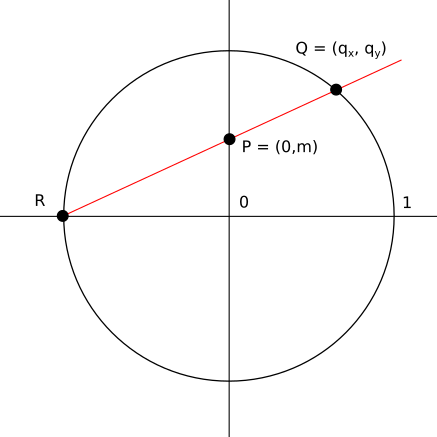
\includegraphics[scale=0.5]{images/rational_point_circle_01.png}
\end{figure}

\subsection{Interpretation}

The key point in the whole derivation is that there is a condition that
the sum of the roots, \(\alpha + \beta\), is rational. Now with the
condition that one root is rational, it follows that the other root is
also rational. If we would not consider a circle (a curve described by
an equation with degree 2), but a curve described by an equation of
higher order, this argument would no longer hold.

%\DiaryEntry{Distance between (Random) Points on Lines}{2016-07-11}{Stochastic}

\subsection{Expected Distance between a fixed Point and a random Point on a Line}

Consider the one-dimensional problem of a point P at \(x=0\) and a line
\(x=L \ldots L+1\). Now choose a random point in uniform fashion on the
line. Let \(d\) denote the random distance between P and the randomly
chosen point. The Figure below shows the problem geometry.

\begin{figure}[H]
\centering
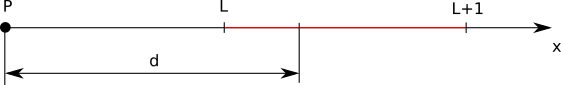
\includegraphics[scale=0.7]{images/expected_distances_01_01.png}
\end{figure}

We want to calculate the expected value of \(d\):

\[
\mathbb{E}(d) = \int_{x=L}^{L+1} x dx = \left. \frac{x^2}{2} \right|_{x=L}^{L+1} = \frac{1}{2} \left[ (L+1)^2 - L^2 \right] = L + 1/2
\]

which is somehow what we expected.

If we consider the expected value of the \emph{squared} distance, we
arrive at

\[
\mathbb{E}(d^2) = \int_{x=L}^{L+1} x^2 dx = \left. \frac{x^3}{3} \right|_{x=L}^{L+1} = \frac{L^3 + 3L^2 + 3L + 1 - L^3}{3} = L(L+1) + \frac{1}{3}
\]

which does not look overly intuitive\ldots{} If we compare
\((\mathbb{E}(d))^2\) and \(\mathbb{E}(d^2)\), we see that
\((\mathbb{E}(d))^2\) is always smaller:

\bee
(L+\frac{1}{2})^2 \leq L(L+1)+\frac{1}{3} \rightarrow L^2 + L + \frac{1}{4} \leq L^2 + L + \frac{1}{3} \rightarrow \frac{1}{4} \leq \frac{1}{3}
\eee

This is due to Jensen's Inequality: For any convex function \(\phi\), we
have \(\phi(\mathbb{E}(X)) \leq \mathbb{E}(\phi(X))\). Since \(()^2\) is
a convex function, the inequality holds.

Also interesting is the fact, that the difference between the two
expectations is constant and independent of L:
\(\mathbb{E}(d^2) - (\mathbb{E}(d))^2 = 1/12\).

\subsection{Expected Distance between two random Points on a Line
(I)}\label{expected-distance-between-two-random-points-on-a-line-i}

Now consider two lines; one at \(x=0 \ldots 1\) and one at
\(x=L \ldots L+1\) with \(L \geq 1\). The Figur below shows the problem
geometry.

\begin{figure}[H]
\centering
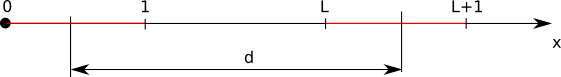
\includegraphics[scale=0.7]{images/expected_distances_01_02.png}
\end{figure}

The expected value of \(d\) is obtain as

\[
\mathbb{E}(d) = \int_{x_2=L}^{L+1} \int_{x_1=0}^{1} x_2 - x_1 dx_1 dx_2
\]

There seems to be no clever trick than to brute force evaluate the
integral. For the inner integral, we obtain

\[
\int_{x_1=0}^{1} x_2 - x_1 dx_1 = \left. x_1 x_2 - \frac{x_1^2}{2} \right|_{x_1=0}^1 = x_2 - \frac{1}{2}
\]

Inserting this into the outer integral, we obtain

\[
\mathbb{E}(d) = \int_{x_2=L}^{L+1} x_2 - \frac{1}{2} dx_2 = \left. \frac{x_2^2}{2} - \frac{x_2}{2} \right|_{x_2=L}^{L+1} = \cdots = L
\]

which is again what we expected.

If we perform the same exercise for the squared distance, we arrive at

\[
\mathbb{E}(d) = \int_{x_2=L}^{L+1} \int_{x_1=0}^{1} (x_2 - x_1)^2 dx_1 dx_2 = \ldots = L^2 + \frac{1}{6}
\]

As above, we have \((\mathbb{E}(X))^2 \leq \mathbb{E}(X^2)\); and again
we have the interesting fact, that the difference between the two terms
is constant and independent of L.

\subsubsection{Overlapping Lines}

In the special case that both lines overlap; i.e.~both lines range from
\(0\) to \(1\), we need to consider the absolute value of the distance:

\bee
\mathbb{E}(|d|) = \int_{x_2=0}^1 \int_{x_1=0}^1 |x_2 - x_1| dx_1 dx_2
\eee

We can get rid of the absolute value in the integral if we split the
integration:

\bee
\mathbb{E}(|d|) = \int_{x_2=0}^1 \left( \int_{x_1=0}^x2 x_2 - x_1 dx_1  +  \int_{x_1=x_2}^1 x_1 - x_2 dx_1 \right) dx_2
\eee

The integration is tedious, but standard and yields
\(\mathbb{E}(|d|) = 1/3\).
\href{http://math.stackexchange.com/questions/195245/average-distance-between-random-points-on-a-line}{Here}
is also a discussion of the problem; there are also several attempts to
provide the intuition behind the answer.

In case we drop the absolute value we obtain \(\mathbb{E}(d) = 0\). This
seems plausible as the problem is symmetric: For any pair \((x_1,x_2)\),
the integral will contain a contribution for \(x_2 - x_1\) and
\(x_1 - x_2\). They will have the same probability but different sign
and will therefore cancel out.

\subsection{Expected Distance between two random Points on a Line (II)}

If the lines are spaced apart in the y-direction, we can also evaluate
the mean (squared) distance. The problem geometry is shown below.

\begin{figure}[H]
\centering
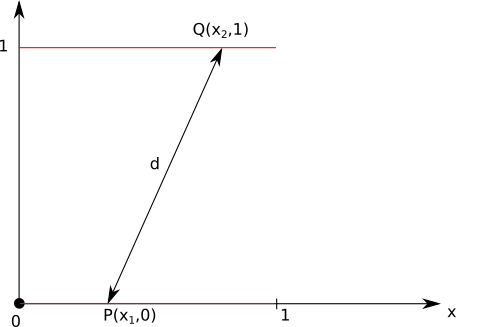
\includegraphics[scale=0.7]{images/expected_distances_01_03.png}
\end{figure}

The distance d between the points P and Q is given by
\(d = \sqrt{(x_2 - x_1)^2 + 1}\) and we obtain for the (simpler)
expected value of the squared distance

\bee
\mathbb{E}(d^2) = \int_{x_2=0}^1 \int_{x_1=0}^1 (x_2 - x_1)^2 + 1 dx_1 dx_2 = \ldots = \frac{7}{6}
\eee

If we are interested in the expected distance itself, we have to solve
the integral

\bee
\mathbb{E}(d) = \int_{x_2=0}^1 \int_{x_1=0}^1 \sqrt{(x_2 - x_1)^2 + 1} dx_1 dx_2 = \ldots = \frac{2-\sqrt{2}}{3} - \log \left( 1 + \sqrt{2} \right)
\eee

but I do not know how sympy was able to solve this integral.

%\DiaryEntry{Coupon Collector Problem}{2016-07-13}{Stochastic}


A source sends out an infinite sequence of coupons and there are \(N\)
different coupons. The same coupon will be sent several times.

We are interested in obtaining a set of \(K\) \emph{different} coupons
(\(K \leq N\)) - What is the expected number of coupons to receive
\(\mathbb{E}(D(N,K))\) in order to have \(K\) different ones? This is
actually a more general question than the coupon collector's problem
where only the expected number of coupons till \(K=N\) different ones
have been observed.

For the first coupon, any coupon will be a new one and therefore
\(\mathbb{E}(D(N,1)) = 1\). For the second new coupon, the process is
started anew: The source sends coupons; with a probability of
\((N-1)/N\) we will receive a new one and with a probability of \(1/N\)
we will receive the one we already have. This is a Bernoulli process and
the expected number of coupons required before a new one is observed is
one over the probability; i.e. \(N/(N-1)\).

In a similar we can argue for the third coupon: The probability to
observe a new one is \((N-2)/N\) and the expected number of coupons to
wait is \(N/(N-2)\).

Therefore in the general case we have

\bee
\mathbb{E}(D(N,K)) = \sum_{k=0}^{K-1} \frac{N}{N-k} = N \sum_{k=0}^{K-1} \frac{1}{N-k}
\eee

For increasing \(K\), more terms in the sum are added and these terms
are increasing - the more different coupons we want to obtain, the
longer we need to wait.

%\DiaryEntry{50 Challenging Problems in Probability, Problem 9 (Craps)}{2016-07-15}{Stochastic}


Consider what happens when we have a sum of 4; called point 4 (btw, this
happens with probability \(P_4 = 3/36 = 1/12\) as there are three
different ways to obtain a sum of \(4\): \(1+3, 3+1, 2+2\) and each
summand has a probability of \(1/36\)): We throw again the two dice and
have 11 outcomes (2\ldots{}12):

\begin{itemize}
\item
  With probability of \(3/36\) (as before) we throw a sum of \(4\)
  again, have won immediately and stop.
\item
  With probability of \(6/36 = 1/6\) (\(1+6, 2+5, 3+4, 4+3, 5+2, 6+1\))
  we throw a sum of \(7\), have lost immediately and stop.
\item
  In all other cases we contine with throwing the dice. The probability
  of doing this is \(P_{R4} = 1 - P_4 - 1/6\) which happens to be
  \(P_{R4} = 3/4\).
\end{itemize}

The (conditional) probability that we win after we have thrown a point
4; i.e.~we throw another point 4, P(win \textbar{} point 4), can be
calculated as follows:

\begin{itemize}
\item
  We immediately throw another point 4 with probability \(P_4\).
\item
  We throw ``something else'' and then a point 4 - this has probability
  \(P_{R4}P_4\)
\item
  We throw ``something else'' two times and then a point 4 - this has
  probability \(P_{R4}^2 P_4\)
\end{itemize}

Therefore the conditional probability P(win \textbar{} point 4) becomes
\(P_4 (1 + P_{R4} + P_{R4}^2 + \cdots = P_4 \frac{1}{1 - P_{R4}} = 1/12 \frac{1}{1 - 3/4} = 1/3\).

There is appearently another (simpler) way to obtain this conditional
probability, called ``reduced sample space''. For this we ignore
\emph{all other} outcomes than the one for immediate win and immediate
loss: There are three good cases (\(1+3, 3+1, 2+2\)) and six bad cases
(\(1+6, 2+5, 3+4, 4+3, 5+2, 6+1\)); therefore the conditional
probability P(win \textbar{} point 4) is \(3/(3+6) = 1/3\).

Given the fact that we obtain a point 4 with probability \(P_4\), we
have the overall probability to win with a point 4 of
\(P_4^2 \frac{1}{1 - P_{R4}} = 1/12 \times 1/3\).

\subsection{Simpler Problem}

Maybe the example with the non-uniform probabilities is a bit
complicated and convoluted. Let's try a simpler one: We have one dice;
when we throw a 1 we win immediately, when we throw a 6 we lose
immediately, and in all other cases, we start again (with throwing the
dice). With a probability of \(1/6\) we win immediately, with a
probability of \(1/6\) we lose immediately, and with probability \(4/6\)
we throw again. In this case, the probabilites for losing, winning, and
continuing are the same.

The probability for winning in the continue case is therefore:
\(1/6 \times 4/6 + 1/6 \times (4/6)^2 + \cdots = 1/6 \times \left[ \frac{1}{1-4/6} - 1\right] = 1/3\).

Therefore the overall probability of winning is \(1/6 + 1/3 = 1/2\) (we
have added the probability of throwing a one).

The simpler way is to solve the problem as folllws: At every instant,
there is one good case (i.e.~we win) by throwing a 1 out of a total of
two cases (throw 1 and throw 6); therefore the probability of winning is
\(1/2\). The other 4 cases (which lead to another dice throw) are not
considered as we ``reduce the sample space''.

\subsection{Finite Problem}

Above problems have in common that they are infinite; i.e.~under certain
conditions (throwing a 2\ldots{}5), the players throws the dice again
and this repeats indefinitely. Things are different when the game stops
after a certain amount of throws; as example consider the following
ruleset:

If the first throw gives a 1, the game is won immediately; if a 6 is
thrown, then the game is lost immediately. In case of throwing
2\ldots{}5, throw the dice again. For the second throw, the same rules
apply. In the third throw, everything but a 1 leads to an immediatey
loss, throwing a 1 leads to an immediatey win; i.e.~the game ends in any
case.

The probability of winning is therefore

\begin{itemize}

\item
  probability of throwing a one in the first throw, \(1/6\)
\item
  plus the probility of throwing a one in the second throw,
  \(4/6 \times 1/6\)
\item
  plus the probability of throwing a one in the third throw,
  \(4/6 \times 4/6 \times 1/6\)
\end{itemize}

which sums to
\(1/6 + 4/6 \times 1/6 + 4/6 \times 4/6 \times 1/6 = 0.35...\). It is
the third throw ending the game which causes the probability to become
less than in the games above.

%\DiaryEntry{Rings - Examples}{2016-07-20}{Algebra}

\subsection{Example $\mZ / 5\mZ$}

As an example consider the ring \(\mathbb{Z}/5\mathbb{Z}\) with the following table for addition (mod-5)

\[
\begin{array}{c|ccccc}
+  & 0 & 1 & 2 & 3 & 4 \\
\hline
0  & 0 & 1 & 2 & 3 & 4 \\
1  & 1 & 2 & 3 & 4 & 0 \\
2  & 2 & 3 & 4 & 0 & 1 \\
3  & 3 & 4 & 0 & 1 & 2 \\
4  & 4 & 0 & 1 & 2 & 3 \\
\end{array}
\]

Every row contains exactely one zero; in other words, every element has exactely one additive inverse and the set with addition forms an abelian group.

The multiplication (mod-5) table looks like this

\[
\begin{array}{c|ccccc}
\times  & 0 & 1 & 2 & 3 & 4 \\
\hline
      0 & 0 & 0 & 0 & 0 & 0 \\
      1 & 0 & 1 & 2 & 3 & 4 \\
      2 & 0 & 2 & 4 & 1 & 3 \\
      3 & 0 & 3 & 1 & 4 & 2 \\
      4 & 0 & 4 & 3 & 2 & 1 \\
\end{array}
\]

Every row (except zero) contains exactely one element 1; this implies that every element apart from zero has exactely one multiplicative inverse.

The set is actually not only a ring but a field as every element has a multiplicative inverse.

\subsection{Example $\mZ/6\mZ$}

As an example of a ring consider the field \(\mathbb{Z}/6\mathbb{Z}\) with the following table for addition

\[
\begin{array}{c|cccccc}
+  & 0 & 1 & 2 & 3 & 4 & 5 \\
\hline
0  & 0 & 1 & 2 & 3 & 4 & 5 \\
1  & 1 & 2 & 3 & 4 & 5 & 0 \\
2  & 2 & 3 & 4 & 5 & 0 & 1 \\
3  & 3 & 4 & 5 & 0 & 1 & 2 \\
4  & 4 & 5 & 0 & 1 & 2 & 3 \\
5  & 5 & 0 & 1 & 2 & 3 & 4 \\
\end{array}
\]

Every element has an additive inverse;i.e. the set forms a group with respect to addition. The multiplication table has the following form

\[
\begin{array}{c|cccccc}
\times  & 0 & 1 & 2 & 3 & 4 & 5 \\
\hline
     0  & 0 & 0 & 0 & 0 & 0 & 0 \\
     1  & 0 & 1 & 2 & 3 & 4 & 5 \\
     2  & 0 & 2 & 4 & 0 & 2 & 4 \\
     3  & 0 & 3 & 0 & 3 & 0 & 3 \\
     4  & 0 & 4 & 2 & 0 & 4 & 2 \\
     5  & 0 & 5 & 4 & 3 & 2 & 1 \\
\end{array}
\]

The rows with element 2, 3, and 4 have more than one zero; i.e.~the element 2 has two multiplicative inverses, namely 3 and 5, because \(2\times3=2\times5=0\). It is exactely the rows with value \(k\) for
which \(\gcd(k,6) \neq 1\) for which no unique multiplicative inverse exists.

However, $\mZ/6\mZ$ is a ring; the set with multiplication need not be a group (and therefore have aninverse).

%\DiaryEntry{Quotient Rings}{2016-07-21}{Algebra}

Let A be a ring with an ideal J; then a coset of the ring is deined as
follows:

\[
J + a = \{j + a: j \in J \} \forall a \in A
\]

I.e. it is the set of all sums \(j+a\) as a remains fixed and \(j\)
ranges over all elements of the ideal. This is very similar to the coset
definition of groups, therefore most of the results can be reused. The
family of cosets \(J+a\) as \(a\) ranges over \(A\) is a partition of
the ring \(A\).

Adding and multiplying cosets works as follows:

\((J + a) + (J + b) = J + (a+b)\)

and

\((J + a) (J + b) = J + (ab)\)

That this works is due to the properties of ideals (in a similar manner
as in the case of cosets and goups).

If we think of the set of all cosets of \(J\) in \(A\) denoted by
\(A/J\). If \(a+J, b+J, c+J,\ldots\) are cosets, then

\[
A/J = \{a+J, b+J, c+J, \ldots \}
\]

and \(A/J\) with coset addition and multiplication as defined above is a
ring and \(A/J\) is a homomorphic image of \(A\).

Finally, we also have a fundamental homomorphism theorem for rings: If
\(f: A \rightarrow B\) is a homomorphism with kernel \(K\), then \(B\)
is isomorphic with \(A/K\).

%\DiaryEntry{Rings - Integral Domains}{2016-07-21}{Algebra}

Integral domains are a commutative ring with unity (i.e.~multiplication
is commutative and there is an identity element for multiplication) in
which the cancellation property holds: In case \(a \neq 0\) and
\(ab = ac\), we can deduce that \(b=c\). The cancellation property is
equivalent to that there are no divisors of zero: If \(ab=0\), then
\(a=0\) or \(b=0\) (or both are zero).

Most prominent example are the integers \(\mathbb{Z}\).

Note that \(\mathbb{Z}/6\mathbb{Z}\) is \textbf{not} an integral domain
as it does not have the cancellation property; e.g. \(2 \times 3=0\). It
is, however, a commutative ring with unity.

A nilpotent element r of a ring R is an element for which
\(e^n=0, n \in \mathbb{N}\) holds. If a ring R has a nilpotent element
\(r \neq 0\), then this element is a divisor of zero. We have \(r^n=0\)
and can rewrite this as \(r r^{n-1}=0\)\$, hence r is a divisor of zero.

\(\mathbb{Z}/16\mathbb{Z}\), \(2^4=0\) and therefore 2 is a divisor of
zero in this ring. Note that a ring may have divisors of zero without
having nilpotent elements (e.g. \(\mathbb{Z}/6\mathbb{Z}\)).

A subring of a field is an integral domain. Examples: Any subring of
\(\mathbb{R}\) or \(\mathbb{C}\) is an integral domain. Thus for example
\(\mathbb{Z}[\sqrt{2}]\) is an integral domain.

\subsubsection{Examples}\label{examples}

Besides the obvious \(\mathbb{Z}\) and \(\mathbb{Z}/p \mathbb{Z}\) being
integral domains, also \(\mathbb{Z}[x]\) is an integral domain. Since
this integral domain is not finite, it is also not a field; i.e.~not
every element has an inverse.

To show that \(\mathbb{Z}[x]\) is an integral domain, we note that the
sum, difference, and product of two elements \(a, b \in \mathbb{Z}[x]\)
is also in \(\mathbb{Z}[x]\). To show that the cancellation property
holds, we define the conjugate of \(a=a_1+a_2x\) as
\(\bar{a} = a_1-a_2x\) and the function \(n(a) = a \bar{a}\). Note that
this function takes elements from \(\mathbb{Z}[x]\) and outputs values
in \(\mathbb{Z}\).

We have \(n(a) = a_1^2 - x^2 a_2^2\) and this is only zero when
\(a_1=a_2=0\); i.e. \(a=0\) (because x is irrational / imaginary). Next
note that \(n(ab) = a \bar{a} b\bar{b} = a\bar{a}b\bar{b} = n(a)n(b)\)
because of the commutative law for multiplication.

Assume that \(ab=0\) and therefore \(n(ab)=0\), from which
\(n(a)n(b)=0\) follows. We therefore have \(n(a)=0\) or \(n(b)=0\) and
from this follows that either \(a=0\) or \(b=0\).

Taken from
\href{www.cut-the-knot.org/arithmetic/int_domain.shtml}{here}.

\subsection{Divisibility of 1 / Unit}\label{divisibility-of-1-unit}

A unit in a commutative ring R is an element that divides 1:
\(uu^{-1}=1\). If every element in R has a unit and R is commutative,
then R is a field. However, there are cases where not every element is a
unit.

\subsubsection{Examples}\label{examples-1}

Taken from
\href{http://www.cut-the-knot.org/arithmetic/int_domain2.shtml}{here}.

I think this stuff holds only for \(\mathbb{Z}[x]\).

If \(u\) is a unit; i.e. \(uu^{-1}=1\), then \(n(u)=\pm 1\).

If \(n(a)=\pm 1\), then \(a\) is a unity. We have \(n(a)=a\bar{a}=1\)
and this shows that \(a\) times ``something'' is 1. Furthermore, if
\(u\) is a unit, then \(u^n, n \in \mathbb{Z}\) is also a unit (We have
\(n(u^2) = n(uu) = n(u)n(u) = 1 1 = 1\).).

In \(\mathbb{Z}[\sqrt{3}]\), the element \(2+\sqrt{3}\) is a unity. We
have

\[
\frac{1}{2+\sqrt{3}} = \frac{2 - \sqrt{3}}{4-3} = 2 - \sqrt{3}
\]

Furthermore, we have \(n(2+\sqrt{3}) = 4 - 3 = 1\). Finally, by squaring
\(2 + \sqrt{3}\) we obtain another unity:
\((2 + \sqrt{3})^2 = 7 + 2\sqrt{3}\).

\subsection{Characteristic of an Integral
Domain}\label{characteristic-of-an-integral-domain}

The (additive) characteristic of a ring with unity is the least positive
integer \(n\) such that \(na =0\). If \(n\) does not exist, then the
ring has characteristic \(0\).

Therefore \(\mathbb{Z}\) has characteristic 0. The ring
\(\mathbb{Z}/5\mathbb{Z}\) in the previous example has characteristic
\(5\), as \(1+1+1+1+1=0, 2+2+2+2+2=0, \ldots\).

\subsubsection{Further Results}\label{further-results}

All non-zero elements in an integral domain have the same (additive)
characteristic: With the characteristic \(n^\star\), we observe that
\(n^\star a = a +a + \cdots + a = 1a + 1a + \cdots + 1a = (1+1+\cdots+1)a = (n^\star 1)a\).
Since we are in an integral domain, \((n^\star 1)a=0\) if
\(n^\star 1=0\) (We consider only nonzero elements, \(a \neq 0\) and in
an integral domain a product is zero, if one or two factors is zero).
Therefore \(n^\star a=0\) and \(a\) has characteristic \(n^\star\).

In an integral domain with non-zero characteristic, the characteristic
is a prime number. If it were a composite number \(mn\), we would have
\(mn = (m1)(n1) = (mn)1 = 0\) and therefore wither \(m1\) or \(n1\)
would be zero. But the characteristic is the \textbf{least} number for
which \(mn1=0\) and this is a contradiction. Therefore, the
characteristic cannot be composite and must be prime.

In an integral domain with characteristic \(p\),
\((a+b)^p = a^p + b^p\). In every commutative ring, the binomial formula
holds, therefore we can expand the expression:

\[
(a+b)^p = a^p + {p \choose 1} a^{p-1} b + \cdots + {p \choose p-1} a b^{p-1} + b^p
\]

If \(p\) is prime and \(0 < k < p\), then \({p \choose k}\) is a
multiple of \(p\) and is therefore zero.

Finally, we have that every finite integral domain is a field. The only
difference between an integral domain and a field is the invertibility
of its elements; in a finite integral domain every element is invertible
so it also a field. The proof is actually quite nice: Asume the integral
domain has the following elements \(0, 1, a_1, a_2, \ldots,a_n\), that
iss \(n+2\) elements. Next note that the products
\(a_i 0, a_i 1, a_i a_1, \ldots, a_i a_n\) are all distinct because if
\(a_i x = a_i y\), then \(x=y\) would follow by the cancellation
property. Therefore, we also have \(n+2\) different products. Since we
have \(n+2\) different domain elements, every domain element is equal to
one of these products. So, \(a_i x = 1\) for some \(x\), there (every)
\(a_i\) is invertible. Note that the proof does not depend on which of
the product actualy equals \(1\); it is enough that the products are
distinct.

%\DiaryEntry{Rings - Integral Domains, 2}{2016-07-26}{Algebra}

The integers are an integral domain, but this definition is not
sufficient, as there are many integral domains which behave rather
differently than the integers. In order to define the integers (and only
the integers), we need to add some more axioms to the integral domain
definitions.

\subsection{Ordered Integral Domain}\label{ordered-integral-domain}

An ordered integral domain is an integral domain with a relation \(<\)
having the following properties:

\begin{itemize}
\item
  For any \(a, b \in A\), one of the following is true: \(a=b\),
  \(a<b\), \(a>b\)
\item
  If \(a<b\) and \(b<c\), then a\textless{}c\$
\item
  If \(a<b\), then \(a+c<b+c\)
\item
  If \(a<b\), then \(ac<bc\) if \(0<c\)
\end{itemize}

The relation allows a definition of positive and negative elements of A.
Furthermore, the square of every non-zero element is positive: If
\(0<c\), then \(0c < c^2 \rightarrow 0<c^2\); if \(c<0\), then
\(0<-c \rightarrow 0(-c) < (-c)^2 = c^2 \rightarrow 0 < c^2\).

The set of all positive elements in \(A\) is denoted as \(A^+\), and an
integral domain is called an integral system if every non-empty subset
of \(A^+\) has a least (smallest) element. This is called the
well-ordering property of \(A^+\).

\(\mathbb{Z}\) is an integral system; e.g.~the least element of all even
numbers is 2. On the contrary, \(\mathbb{Q}\) is not an integral system;
e.g.~the subset \(0<x<1\) has no least element (for every fraction
\(m/n\), there always exists a smaller fraction).

In any integral system there is no element between 0 and 1. Proof by
contradiction - assume that \(0<x<1\). Then the set
\(\{x \in A, 0<x<1\}\) is a non-empty positive set so it has a least
element \(c\) by the well-ordering property. So \(0<c<1\) and if we
multiply with \(c\), we obtain \(0<c^2<c\). We can now combine the 2
inequalities and obtain \(0<c^2<c<1\). This does not seem to be possible
ands we have a contradiction\ldots{}??

In any integral system, all elements are multiplies of 1 and ordered
exactely as in \(\mathbb{Z}\). Therefore, every integral system is
isomorphic to \(\mathbb{Z}\). From this we conclude that any two
integral systems are isomorphic to eah other and therefore
\(\mathbb{Z}\) is the *only\$ integral system (the others are all
isomorphisms).

\subsection{Induction}\label{induction}

The proof by induction method is based on a simple fact of the positive
integers. If \(\mathbb{K}\) is a set of positive integers, and

\begin{itemize}
\item
  if \(1 \in \mathbb{K}\), and
\item
  for any positive \(k \in \mathbb{K}\), then \(k+1 \in \mathbb{K}\)
\end{itemize}

If \(\mathbb{K}\) satisfies these conditions, then \(\mathbb{K}\)
consists of all the positive integers.

Assume we have a statement \(S_n\) about a positive integer \(n\).
Induction then works by starting with \(S_1\) being true, and deducing
that \(S_{n+1}\) is true when \(S_n\) is true. If these conditions hold,
then \(S_n\) is true for every positive integer.

\subsection{Division Algorithm}\label{division-algorithm}

If \(m,n\) are integers and \(n\) is positive, there exist unique
integers \(p,q\) such that

\[
m=nq + r , \quad 0 \leq r < n
\]

%\DiaryEntry{Rings - Structure of Ideals}{2016-07-26}{Algebra}

A \emph{principal ideal} \(\langle a \rangle\) of \(\mathbb{Z}\) is
defined as follows:

\[
\langle a \rangle = \{ax\}
\] with \(a\) fixed in \(\mathbb{Z}\) and \(x\) ranging over all
\(\mathbb{Z}\). For example,
\(\langle 3 \rangle = \{\ldots, -9, -6, -3, 0, 3, 6, 9, \ldots\}\).

We have the fact that every ideal of \(\mathbb{Z}\) is principal.

\subsection{Divisibility}\label{divisibility}

If \(r, s\) are integers and \(s = rk\) with integer \(k\), then s is a
multiple of \(r\) or \(r\) is a factor of \(s\), or \(r\) divides \(s\).
We can further symbolize this as \(r | s\).

The only invertible elements of \(\mathbb{Z}\) are \(1\) and \(-1\);
i.e.~to have \(rs=1\), \(r=1\) or \(r=-1\) for \(s \in \mathbb{Z}\).

An integer pair \((r,s)\) is called associative, if the integers divide
each other; i.e. \(r|s\) and \(s|r\). If r and s are associates, then
\(r = \pm s\).

If an integer \(t\) divides both \(r\) and \(s\); i.e. \(t|r, t|s\),
then \(t\) is called a common divisor of \(r\) and \(s\). The greatest
common divisor \(\gcd(r,s)\) divides both \(r\) and \(s\) and every
other common divisor of \(r\) and \(s\) divides \(t\):
\(\gcd(r,s) | r, \gcd(r,s) | s\) and for any integer \(u\), if \(u|r\)
and \(u|s\), then \(u|t\).

The term greatest in the gcd means not necessarily ``greater in
magnitude'', but merely ``divides any other gcd''.

Any two non-zero integers r and s have a gcd t. This t is equal to a
linear combination of r and s as

\[
t = kr + ls
\]

for some integers k and l.

Proof: Let J be the set of all linear combinations of r and s;
\(J=\{ur+vs\}\) as u and v range over \(\mathbb{Z}\). J is closed with
respect to addition, and negatives, and absorbs products
(\(w(ur+vs) = (wu)r + (wv)s\)). Therefore J is an ideal of
\(\mathbb{Z}\); but since every ideal is a principal one, we can also
write \(J=\langle t \rangle\) for some t. Since t is in J, it is also a
linear combination of r and s: \(t = kr + ls\). r and s are also linear
combinations of r and s, therefore r and s are also in J. All elements
of J are multiples of t, so r and s are multiples of t; i.e.
\(t|r, t|s\). If u is a common divisor of r and s, we have
\(r=xu, s=yu\) for some integers x and y. Thus

\[
t = kr + ls = kxu + lyu = u(kx + ly)
\]

and from this follows that \(u|t\). From this follows that t is the gcd
of r and s.

\subsection{Primality and Factorization into
Primes}\label{primality-and-factorization-into-primes}

Two numbers r and s are relatively prime, if their gcd is 1. In other
words, we have \(kr + ls = 1\) for some integers k and l. This holds
also in the reverse direction: If \(kr + ls = 1\), then r and s are
relatively prime.

If an integer m has other factors than the trivial factors \(\pm 1\) and
\(\pm m\), these are called proper factors of m and m is called
composite. We have

\[
m = rs, \quad 1 < r < m, 1 < s < m
\]

If m and n are integers and p is a prime. If \(p|(mn)\), then either
\(p|m\) or \(p|n\).

Proof: If \(p|m\) then we are done. If p does not divide m, then we
proceed as follows: The only divisors of p are \(\pm 1\) and \(\pm p\).
Since p does not divide m, \(\pm p\) are ruled out as common divisors of
p and m; their only common divisors are \(\pm 1\).

Therefore \(\gcd(p,m=1\) and we can write \(kp + lm = 1\) (for some
integers k,l) by the previous theorem. Multiplying with n yields
\(kpn + lmn = n\). We assumed that \(p|(mn)\), so \(mn = ph\) (for some
integer h). So we can write \(kpn + lph = n \rightarrow p(kn + lh) = n\)
and therefore \(p|n\).

This can be extended to products with more than two factors: if
\(p|(m_1 \ldots m_t)\), then \(p|m_i\) for one of the factors. If the
factors \(m_1,\ldots,m_t\) are all positive primes, then p must equal
one of them.

Every integer \textgreater{} 1 can be expressed as product of positive
primes.

Proof: Let the set K represent positive integers \textgreater{} 1 which
cannot be written as product of one or more primes. By well-ordering, K
contains a least integer m which is not be prime (if it were, it would
not be in K). So m is composite, and we have \(m = rs\) for
\(1 < r,s < m\). The r and s are not in K because m is the least integer
in K. This means that r and s can be expressed as product of primes and
therefore also \(m=rs\). This is a contradicton (we assumed that m is
the smallest integer which cannot be expressed as product of one or more
primes) and therefore every \(n>1\) can be expressed as product of one
or more primes.

The prime factorization is unique.

Proof: Assume that \(m = p_1 \cdots p_r = q_1 \cdots q_t\) and cancel
common factors from each side until no more cancelling is possible. If
all factors cancel, we are done and factorization is unique. Otherwise,
we are left with an expression of the form

\[
p_i \cdots p_k = q_j \cdots q_m
\]

from which we deduce that \(p_i | q_j \cdots q_m\). The q's are all
prime, therefore \(p_i\) must be equal to one of them (see above). But
this is impossible since we assumed that no more cancelling is possible.

%\DiaryEntry{Polynomials, I}{2016-07-26}{Algebra}

Let \(A\) be a commutative ring with unity and \(x\) an arbitrary
symbol. Then an expression of the form

\[
a_0 + a_1 x + a_2 x^2 + \cdots + a_n x^n
\]

is a polynomial in x with coefficients in A.

\subsection{Operations}\label{operations}

Polynomials can be added (element-wise addition of the coefficients) and
multiplied (convolution of polynomial coefficients).

If \(A\) is a ring, then \(A[x]\) denotes the set of all polynomials in
\(x\) whose coefficients are in \(A\) and addition and multiplication
defined as above.

Then we have:

\begin{itemize}
\item
  If \(A\) is a commutative ring with unity, then \(A[x]\) is also a
  commutative ring with unity.
\item
  If \(A\) is an integral domain, then \(A[x]\) is also an integral
  domain (also called a domain of polynomials).
\end{itemize}

In case \(F\) is a field, then \(F[x]\) is not necessarily a field as
the multiplicative inverse of a polynomial is not always a polynomial.
However, \(F[x]\) is an integral domain.

\subsubsection{Polynom Division}\label{polynom-division}

If \(a(x), b(x)\) are polynomials over a field \(F\) and
\(b(x) \neq 0\), there exist polynomials \(p(x), r(x)\) over \(F\) such
that

\[
a(x) = b(x) q(x) + r(x)
\]

and \(r(x)=0\) or \(\text{deg} r(x) < \text{deg} b(x)\).

\subsection{Factoring Polynomials}\label{factoring-polynomials}

Let \(a(x)\) and \(b(x)\) be in \(F[x]\). We say \(b(x)\) is a multiple
of \(a(x)\), if \(b(x) = a(x) s(x), s(x) \in F[x]\). We can also write
\(a(x)|b(x)\).

Every non-zero constant polynomial divides every polynomial.

A polynomial \(a(x)\) is invertible iff it is a divisor of the unity
polynomial 1. But if \(a(x)b(x)=1\), then both polynomials have degree 0
and are therefore constant; i.e. \(a(x)=a, b(x)=b, ab=1\). Therefore,
the invertible polynomials of \(F[x]\) are the non-zero constant
polynomials.

Two polynomials are associates iff they are constant multiples of each
other: We can write \(a(x) = b(x)c(x), b(x) = a(x)d(x)\) for some
\(c(x), d(x)\). But then we have \(a(x) = b(x)c(x) = a(x)d(x)c(x)\) and
\(c(x)d(x)=1\) because \(F[x]\) is an integral domain. Therefore,
\(c(x), d(x)\) are constant polynomials, and therefore \(a(x), b(x)\)
are constant multiples of each other.

A polynomial with leading coefficient 1 is called monic. Every non-zero
polynomial has a unique monic associate. As an example consider
\(a(x)=1+3x\). Then the monic associate is \(b(x) = 1/3 + x\) and we
have \(a(x) = 3b(x)\).

In a similar spirit as before we define a gcd \(d(x)\) of two
polynomials \(a(x), b(x)\): \(d(x)|a(x), d(x)|b(x)\) and if
\(u(x)|a(x)\) and \(u(x)|b(x)\), then \(u(x)|d(x)\). Therefore, two gcds
divide each other; we select \emph{the} gcd of \(a(x), b(x)\) as the
monic one. This gcd is unique and can be expresed as linear combination
\(d(x) = r(x)a(x) + s(x)b(x)\) with \(r(x), s(x) \in F[x]\).

A polynomial \(a(x)\) is \textbf{reducible} over \(F[x]\) if
\(a(x)=b(x)c(x), b(x), c(x) \in F[x]\). Each of the two factors has a
degress less than the degree of \(a(x)\). A polynomial is
\textbf{irreducible over F} if it cannot be expressed as product of two
polynomials in \(F[x]\).

It is important to state the field the polynomial is irreducible;
\(x^2+1\) is irreducible over \(\mathbb{R}\), but reducible over
\(\mathbb{C}: x^2+1 = (x+j)(x-j)\).

As before, there are theorems that polynoms can be uniquely factored
into irreducible monic polynomials:

\[
a(x) = k p_1(x) \cdots p_m(x), \quad k \in F, p_1(x), \ldots,p_m(x) \in F[x]
\]

\subsubsection{Examples}\label{examples}

The polynomial \(x^4-4\) can be factored over the field
\(\mathbb{Q}[x]\) as \(x^4-4 = (x^2-2)(x^2+2)\). If we factor over
\(\mathbb{R}[x]\) we can continue as
\(x^4-4 = (x^2+2)(x+\sqrt{2})(x-\sqrt{2})\) and if we finally factor
over \(\mathbb{C}[x]\), we obtain
\(x^4-4 = (x+j\sqrt{2})(x-j\sqrt{2})(x+\sqrt{2})(x-\sqrt{2})\).

%\DiaryEntry{Polynomials, II}{2016-07-27}{Algebra}

\subsection{Polynom Evaluation}\label{polynom-evaluation}

Assume the polynom coefficients come from the field F, then the polynoms
also form a field F{[}x{]} (see previous post).

Assume we have a polynom \(a(x)\) and we insert for the dummy variable x
a value c from F: In this case, we obtain an arithmetic expression which
we can evaluate and which will produce a value in F. The evaluation
involves multiplication and addition of elements from F. The resulting
expression is the polynom value and denoted as \(p(c)\).

\subsubsection{Examples}\label{examples}

Since I repeatedly fell over the modulo operation, let's try a few
examples with \(\mathbb{Z}/5\mathbb{Z}\). Here everything is modulo-5
and we have \(3 \bmod 5 = 3, 6 \bmod 5 = 1\). That's easy. But
\(-1 \mod 5 = 4\) because \(-1 = -1 \times 5 + 4\). Continuing we have
\(-2 \mod 5 = 3, -3 \bmod 5 = 2, -4 \bmod 5 = 1, -5 \bmod 5 =0\). And then
$-6 \bmod 5 = 4$, $-9 \bmod 5 = 1$ because $-6 = -2 \times 5 + 4, -9 = -2 \times 5 + 1$.

As a first example for polynom evaluation, consider \(a(x) = x^2-1\). We
have the following values:
\(a(0) = -1 = 4, a(1) = 0, a(2) = 3, a(3) = 9 \bmod 5 -1 = 4-1=3, a(4) = 16 \bmod 5 - 1 = 1 - 1 = 0\).

A more complicated example is \(b(x) = x^4 - 3x^2 + 1\) which evaluates
as follows:
\(a(0) = 1, a(1) = -1 \bmod 5 = 4, a(2) = 2^4 - 3 2^2 + 1 = 16 - 3\times 4 + 1 = 5 \bmod 5 = 0, a(3) = 3^4 - 3 4^2 + 1 = 55 \bmod 5 = 0, a(4) = 4^4 - 3 4^2 + 1 = 256 - 48 + 1 \bmod 5 = 209 \bmod 5 = 4\).
Note that we can evaluate the polynom ``normally'' and take the mod-5 at
the very end of the computation.

\subsection{Roots of Polynoms}\label{roots-of-polynoms}

If \(a(c)=0\), then c is called a root of the polynom \(a(x)\). This is
equivalent that the polynom \(a(x)\) has a factor \(x-c\).

Proof: We can write \(a(x) = q(x)(x-c) + r(x)\) with \(q(x), r(x)\)
being some polynoms. The remainder \(r(x)\) is either 0 or a polynom of
lower degree than \((x-c)\). But this means that \(r(x)\) is a constant;
i.e. \(r(x) = r\). Therefore we have

\[
0 = a(c) = (c - c)q(c) + r = 0 + r = r
\]

Therefore \(r=0\) and \((x-c)\) is a factor of \(a(x)\).

We can extend this; if a polynom has roots \(c_1, \ldots,c_n\), then
\((x-c_1)\cdots(x-c_n)\) is a factor of the polynom. Therefore, if
\(a(x)\) has degree n, it has at most n roots. The number of roots
depend on the polynom and the field we are considering; e.g. \(x^2+1\)
has \textbf{no} roots in \(\mathbb{Z}\).

\subsubsection{Examples}\label{examples-1}

Things get interesting / counterintuitive, when we consider polynom
factorization over non-\(\mathbb{Z, Q}\) domains. One method of finding
roots which always works is computing all polynom values \(a(x)\) and
checking whether \(a(x)=0\) for some \(x\).

Now consider the first polynom from before, \(a(x) = x^2-1\). Having
zeros at \(x=1\) and \(x=4\), we can rewrite it as
\(a(x) = (x-1)(x-4)\). Multiplying this out gives
\(a(x) = x^2 - 5x + 4 \bmod 5 = x^2 + 4\). Note that \(4 = -1 \bmod 5\),
so we can write the polynom also as \(a(x) = x^2-1\).

Next, the second polynomial from above \(b(x) = x^4 - 3x^2 + 1\). From
the evaluation above, we see that the zeros are 2 and 3; therefore we
can write this as \((x-2)(x-3)\). However, this can't be it, because the
polynom degrees do not match. So we have three different options
\(b_1(x) = (x-2)^3(x-3), b_2(x) = (x-2)^2(x-3)^2, b_3(x) = (x-2)(x-3)^3\)
which we need to evaluate for x=0\ldots{}4 and compare with the values
from \(b(x)\). It turns out that the correct factorization is
\((x-2)^2(x-3)^2\).

Using the modulo relations from above, we have
\(-2 = 3 \bmod 5, 3 = -2 \bmod 5\) and therefore there are several ways of
writing this polynom:
\(b(x) = (x-2)^2 (x-3)^2 = (x+3)^2 (x-3)^2 = (x-2)^2 (x+2)^2 = (x+3)^2(x+2)^2\).
Expanding the expressions and taking all coefficients modulo-5 shows
that the factorizations are all equivalent.

We can do this in SymPy as follows

\begin{verbatim}
import smypy as sym
x=sym.var('x')

sym.factor(x**4-3*x**2+1, modulus=5)

>>> (x - 2)**2*(x + 2)**2
\end{verbatim}

\subsection{Polynom Equality}\label{polynom-equality}

Two polynoms are defined to be equal if their coefficients are equal;
two functions are defined to be equal, if they attain the same values
for every value in their domain. In case of fields with inifinite
elements, these definitions coincide; however in case of finite fields,
the two definitions may lead to different results.

Example: Consider \(a(x) = x^5 + 1\) and \(b(x) = x - 4\). Over
\(\mathbb{Z}_5\), the two polynoms give the same results; i.e.
\(a(1) = b(1), \ldots a(4) = b(4)\). However the coefficients of the two
polynoms are different.

\subsection{\texorpdfstring{Polynoms over
\(\mathbb{Z,Q}\)}{Polynoms over \textbackslash{}mathbb\{Z,Q\}}}\label{polynoms-over-mathbbzq}

If we have a polynom with rational coefficients, we can bring it into a
form polynom with integer coefficients times a rational factor:

\[
a(x) = \frac{1}{2} x^2 + \frac{3}{4} = 4 (2x^2 + 3) = k b(x)
\]

This new polynom has the same roots as the original one. Therefore, it
suffices to consider polynoms with integer coefficients.

Finding their roots can be done as follows. If \(s/t\) is a rational
number in simplest form (\(\gcd(s,t)=1\)) and the polynom has the form
\(b(x) = a_0 + \cdots + a_n x^n\) (with the \(a_i\) being integers), we
have: If \(s/t\) is a root of \(a(x)\), then \(s|a_0\) and \(t|a_n\).

\textbf{Caution}: Note this procedure produces solution candidates. The
polynom can have non-rational roots as well and maybe \emph{all} roots
are non-rational and/or complex. In this case, none of the solution
candidates are actual solutions.

Proof: Obviously we have \(a_0 + s/t a_1 + \cdots (s/t)^n a_n = 0\) and
multiplying both sides with t\^{}n yields
\(a_0 t^n + s t^{n-1}a_1 + \cdots + s^n a_n =0\). We can rearrange that

\[
s \left( t^{n-1} a_1 + \cdots + s^{n-1} a_n \right) = - a_0 t^n
\]

From this follows that \(s | a_0 t^n\) and since s and t have no common
factors, s and \(t^n\) have no common factors, and therefore we have
\(s|a_0\). In a similar spirit, we can factor out t and obtain the other
half of the result; i.e. \(t|a_n\).

Example:

\begin{itemize}
\item
  Consider the polynom \(2x^2+5x-3\). With \(s|-3, t|2\), we have the
  following candidates for roots (all combinations \(s/t\)) :
  \(\pm 1/2, \pm 1, \pm 3/2, \pm 3\). Inserting these values into the
  polynom shows that the two roots are \(1/2\) and \(-3\).
\item
  Consider \(x^3-2x^2+x-2\). \(s|-2, t|1\) and therefore the possible
  root candidates are \(\pm 1, \pm 2\). Inserting into the polynom shows
  that \(2\) is a root. The other roots are \(\pm j\) which are
  non-rational solutions and are therefore not found with this method.
\end{itemize}

If we have a product of polynoms with \(a(x) = b(x)c(x)\) and a prime
number p divides every coefficient of \(a(x)\), it either divides every
coefficient of \(b(x)\) or every coefficient of \(c(x)\).

Since every polynom with rational coefficients can be expressed as a
rational factor times a polynom with integer coefficients, we have: If
\(a(x) = b(x)c(x)\) with \(b(x), c(x)\) having rational coefficients,
then there are polynoms \(B(x), C(x)\) which are constant multiples of
\(b(x), c(x)\), respectively, such that \(a(x) = B(x) C(x)\).

Stated differently, every polynom which is reducible over \(\mathbb{Q}\)
is reducible already over \(\mathbb{Z}\).

\subsection{Eisensteins Criteria}\label{eisensteins-criteria}

Let

\[
a(x) = a_0 + a_1 x + \cdots a_n x^n
\]

be a polynom with integer coefficients. If there is a prime p which
divides every coefficient except \(a_n\) and p does \emph{not} divide
\(a_n\) and \(p^2\) does \emph{not} divide \(a_0\). Then \(a(x)\) is not
reducible over \(\mathbb{Q}\).

As an example consider \(x^3 + 2x^2 + 4x + 2\). If we set \(p=2\), \(p\)
divides every coefficient except \(a_n=1\) and \(p^2=4\) does not divide
\(a_0=2\). Therefore \(a(x)\) is irreducible over \(\mathbb{Q}\).

We can use Eisenstein's Criteria to show that
\(a(x) = x^{p-1} + x^{p-2} + \cdots + x + 1\) is irreducible over
\(\mathbb{Q}\) if is p is a prime.

We can rewrite

\[
a(x) = \frac{x^p-1}{x-1} = \frac{(y+1)^p-1}{y}
\]

where have used the substitution \(y=x+1\). This does not change the
results about reducibility for if \(a(x) = b(x)c(x)\) we have
\(a(x+A) = b(x+A)c(x+A)\). Now expand the expression with the binomial
formula

\[
a(x) = \frac{\sum_{n=0}^p {p \choose n} y^n - 1}{y} = \frac{\sum_{n=1}^p {p \choose n} y^n}{y} = \sum_{n=1}^p {p \choose n} y^{n-1} = \sum_{n=0}^{p-1} {p \choose n+1} y^n
\]

We can now apply Eisensteins criteria: The highest and lowest
coefficients are zero \(a_n = a_0=1\), all others are divisible by p
(since it is prime). Obviously, p does not divide \(a_n=1\), neither
does \(p^2\) divide \(a_0=1\). Therefore \(a(x)\) is irreducible over
\(\mathbb{Q}\).

%\DiaryEntry{Binomial Expansion}{2016-08-01}{Algebra}

Based on
\href{http://math.stackexchange.com/questions/1869954/expansion-of-1-sqrt2n}{this
question}.

Consider the expression \((1+\sqrt{2})^n, n \in \mathbb{N}\) and expand
it via the binomial formula:

\[
(1+\sqrt{2})^n = \sum_{k=0}^n {n \choose k} (\sqrt{2})^k = a_n + b_n \sqrt{2}
\]

Note that the terms with k being even become integers: \({n \choose k}\)
is integer and \((\sqrt{2})^k\) is an integer (namely \(2^{k/2}\)) for k
even. The \(a_n, b_n\) collect all these term.

We can do the same for the expression

\[
(1-\sqrt{2})^n = \sum_{k=0}^n {n \choose k} (-1)^k (\sqrt{2})^k
\]

In addition to the observation above, we note that
\((-1)^k (\sqrt{2})^k = 2^{k/2}\) for k even and
\((-1)^k (\sqrt{2})^k = -(\sqrt{2})^k\) for k odd. Therefore, we can
write

\[
(1-\sqrt{2})^n = a_n - b_n \sqrt{2}
\]

Collecting things, we have


\begin{align*}
(1-\sqrt{2})^n &= a_n - b_n \sqrt{2} \\
(1+\sqrt{2})^n &= a_n + b_n \sqrt{2}
\end{align*}


This can be extended according to


\begin{align*}
(a-b\sqrt{2})^n &= a_n - b_n \sqrt{2} \\
(a+b\sqrt{2})^n &= a_n + b_n \sqrt{2}
\end{align*}


which is a rather nice result: If we consider \(A = a+b\sqrt{2}\) as an
element of \(\mathbb{Z}[\sqrt{2}\), then \(A^n\) is also in this ring;
i.e.~taking it to the n-th power does \emph{not} introduce any new
irrational numbers.

We can multiply the left parts and the right parts with each other to
obtain

\[
a_n^2 - 2b_n^2 = (1-2)^n = (-1)^n
\]

So we see that the \emph{absolute} difference between \(a_n^2\) and
\(2b_n^2\) is one. If we arrange this to get an expression for
\(b_n \sqrt{2} = \sqrt{a_n^2-(-1)^n}\) and insert this into
\(a_n + b_n \sqrt{2}\) we obtain

\[
(1+\sqrt{2})^n = a_n + b_n \sqrt{2} = \sqrt{a_n^2} + \sqrt{a_n^2 - (-1)^n}
\]

which is (more or less) the result from the post.

%\DiaryEntry{Field Extensions, I}{2016-08-05}{Algebra}

If F is a field, then a subfield K is a non-empty subset of F which is
closed with respect to addition, subtraction, multiplication, and
division. In other words, K is a field in its own right.

If we reverse our point of view, we can also say that F is a field
extension of K.

If F is an arbitrary field, there are, in general, polynomials over F
which have no roots in F. More exactely, every polynomial of degree n
has n roots, but they \textbf{need not} necesarily be in F. However, one
can show that the n roots are contained in a suitable extension E of F.

We can group the elements of E into two groups: \emph{Algebraic}
elements of E are elements which are roots of non-zero polynomials in
F{[}x{]}. \emph{Transcendental} elements of E are all the others;
i.e.~elements which are not roots of any polynomials in F{[}x{]}.

If we consider \(\mathbb{Q}\), then an extension field is
\(\mathbb{R}\): The polynomial \(x^2-2\) has no roots in \(\mathbb{Q}\);
however \(\pm \sqrt{2} in \mathbb{R}\). So for this polnomial,
\(\mathbb{R}\) is a suitable extension field. However, it is not the
``minimum'' extension field; i.e.~it contains elements which are not
roots of \(x^2-2\), e.g. \(\sqrt{3}\). The ``minimum'' extension field
would be \(\mathbb{Q}(\sqrt{2})\).

Transcendental elements are \(\pi\); there is no polynomial in
\(\mathbb{Q}[x]\) which has \(\pi\) as its root (non-trivial statement).

\subsubsection{Substitution Function / Evaluation
Homomorphism}\label{substitution-function-evaluation-homomorphism}

For now consider a field F with extension field E.

We define a substitution function (also called evaluation homomorphism)
\(\sigma_c\) for a polynomial s\(a(x) \in F[x]\) as
\(\sigma_c(a(x)) = a(c)\) with \(c \in E\); i.e.~it replaces the free
variable \(x\) with the constant value \(c\). This function maps
elements from \(F[x]\) onto E and is a homomorphism:
\(\sigma_c(a(x) + b(x)) = \sigma_c(a(x)) + \sigma_c(b(x))\) and
\(\sigma_c(a(x)b(x)) = \sigma_c(a(x)) \sigma_c(b(x))\).

The kernel of \(\sigma_c\) is the set of all polynomials \(a(x)\) so
that \(a(c) = \sigma_c(a(x)) = 0\). In other words, the kernel contains
all polynomials \(a(x)\) having a root \(c\). Let us denote the kernel
of \(\sigma_c\) by \(J_c\). \(J_c\) is an ideal; moreover in \(F[x]\)
every ideal is a principal ideal and so \(J_c\) is also a principal
ideal. Therefore \(J_c = \langle p(x) \rangle\) is the set of all
multiples of \(p(x)\). \(p(x)\) is the polynomial with lowest degree of
all nonzero polynomials in \(J_c\) and \(p(x)\) is irreducible. We can
further constrict \(p(x)\) to be a monic polynomial and all together
\(p(x)\) is an irreducible monic polynomial of lowest degree in \(J_c\)
with root \(c\). It is called the minimum polynomial.

As an example consider the substitution function \(\sigma_{\sqrt{2}}\);
i.e.~the function which substitutes \(\sqrt{2}\) into \(x\). E.g.
\(\sigma_{\sqrt{2}}(x^2-1) = \sqrt{2}^2-1 = 1\). By the previous
discussion, the kenel of the homomorphism \(\sigma_{\sqrt{2}}\) contains
all polynomials with one of the roots being \(\sqrt{2}\). The minimum
polynomial is \(p(x) = x^2-1\): It is monic, nonzero, and is has lowest
degree of all polynomials which have \(\sqrt{2}\) as one of their roots.
The ideal \(J_c = \langle x^2-1 \rangle\) is the set of all polynomials
\(J_c = \{(x^2-1) a(x), a(x) \in F[x]\}\). From this definition we can
see that all elements from this ideal have a root at \(x=c\) (the first
factor is zero).

The range of \(\sigma_c\) is closed with respect to addition,
multiplication, and negatives (this follows from \(\sigma_c\) being a
homomorphism. However, it is also closed to multiplicative inverses
(this is evident and needs to be proven).

Therefore, the range of \(\sigma_c\) is a subfield of E and is given as
the set of all elements \(a(c)\) for all \(a(x) \in F[x]\). It is also
the \emph{smallest field containing both F and c}. By smallest we mean
the field which contains F and c and is contained in any other field
containing F and c. It is called the \emph{field generated by F and c}
and is denoted by \(F(c)\). By the fundamental homomorphism theorem,
\(F(c)\) is isomorphic to \(F[x] / \langle p(x) \rangle\).

Summarizing, if \(p(x)\) is an irreducible polynomial in \(F[x]\), then
\(F(c)\) is a suitable field extension to F; i.e.~it contains a root of
\(p(x)\) and \(F(c)\) is isomorphic to \(F[x] / \langle p(x) \rangle\).

\subsection{Vector Spaces and Field
Extensions}\label{vector-spaces-and-field-extensions}

Let F and K be fields and K an extension field over F. We may consider
the elements of K as vectors, whereas the elements of F are scalars.
Adding elements of K amounts to vector addition, adding and multiplying
elements of F can be thought in terms of scalar addition and
multiplication. Multiplying an element of F with one of K can be thought
of multiplying a scalar with a vector.

Especially interesting is the case of vector spaces with finite
dimension. If K - as a vector space- is of finite dimension, we call K a
finite extension of F. If the vector space dimension of K is n, then K
is an extension of degree n over F. We write this as

\[
[K:F] = n
\]

If c is algebraic over F and let \(p(x)\) be the minimum polynomial of c
over F. Let the degree of \(p(x)\) be n. Then, the elemnts

\[
1, c, c^2, \ldots, c^{n-1}
\]

are linearly independent and span \(F(c)\).

Proof: Any \(a(c)\) is an element of \(F(c)\), we can divide \(a(x)\) by
\(p(x)\): \(a(x) = p(x) q(x) + r(x)\) with the degree of \(r(x)\) less
or equal \(n-1\). Therefore, \(a(c) = p(c) q(c) + r(c) = r(c)\) because
- by the very definition - \(p(c) = 0\). This shows that every element
of F(c) can be written in the form of

\[
a_0 + a_1 c + a_2 c^2 + \cdots + a_{n-1} c^{n-1}
\]

which is a linear combination of \(1, c, c^2, \ldots, c^{n-1}\);
i.e.~these elements form a basis for \(F(c)\). To prove that
\(1, c, c^2, \ldots, c^{n-1}\) are linearly independent, suppose that
\(a_0 + a_1 c + a_2 c^2 + \cdots + a_{n-1} c^{n-1} = 0\). If the \(a_i\)
coefficients were not all zero, c would be the root of a polynomial of
degree n-1 or less, which is impossible because the minimum polynomial
of c over F has degree n. Thus the \(a_i\) must be all zero and
therefore the \(1, c, c^2, \ldots, c^{n-1}\) are independent.

\subsubsection{Example}\label{example}

Consider \(\mathbb{Q}(\sqrt{2})\) with \(\sqrt{2}\) not being a root of
any monic polynomial of degree 1 over \(\mathbb{Q}\). This would be the
polynomial \(x-\sqrt{2}\) and is not in \(\mathbb{Q}[x]\). But,
\(\sqrt{2}\) is the root of \(x^2-2\) which is therefore the minimal
polynomial over \(\mathbb{Q}\) and therefore
\([\mathbb{Q}(\sqrt{2}) : \mathbb{Q}] = 2\).

The elements \(1, \sqrt{2}\) form a basis for \(\mathbb{Q}(\sqrt{2})\);
i.e.~we can write every element of this field as
\(a + b\sqrt{2}, ab,b \in \mathbb{Q}\).

\subsection{Connection between Field Extensions and
Degree}\label{connection-between-field-extensions-and-degree}

If the field E is a finite extension of K and K is a finite extension of
F, then E is also a finite extension of F and we have

\[
[E:F] = [E:K] [K:F]
\]

If \(a_1, a_2, \ldots, a_m\) is a basis of the vector space K over F and
\(b_1, b_2, \ldots, b_n\) is a basis of the vector space E over K, then
the set of mn products \(\{a_i b_j\}\) is a basis for the vector space E
over F.

If c is algebraic over F, then we say that F(c) is constructed from F by
\emph{adjoining} c to F. If both c and d are algebraic over F, then we
can first adjoin F with c, obtain F(c), and then adjoin d to F(c) to
obtain F(c,d). The order of the adjoin operations does not matter. The
resulting F(c,d) then contains all roots c and d.

\subsubsection{Example}\label{example-1}

If we expand the example of \(\mathbb{Q}(\sqrt{2})\) with \(\sqrt{3}\),
we observe that \(\sqrt{3}\) cannot be expressed in
\(\mathbb{Q}(\sqrt{2})\): \(\sqrt{3} = a + b\sqrt{2}\) can not be
fulfilled with \(a,b \in \mathbb{Q}\). However, \(\sqrt{3}\) is a root
of \(x^2-3\) which is therefore a minimum polynomial in
\(\mathbb{Q}(\sqrt{2})\). Therefore \(\mathbb{Q}(\sqrt{2}, \sqrt{3})\)
is therefore degree 2 over \(\mathbb{Q}(\sqrt{2})\) and therefore
\(\mathbb{Q}(\sqrt{2}, \sqrt{3})\) is of degree 4 over \(\mathbb{Q}\).
The elements \(\{1, \sqrt{2}\}\) are a basis for
\(\mathbb{Q}(\sqrt{2})\) and the elements \(\{1, \sqrt{3}\}\) are a
basis for \(\mathbb{Q}(\sqrt{2}, \sqrt{3})\). Therefore,
\(\{1, \sqrt{2}, \sqrt{3}, \sqrt{2 \cdot 3} = \sqrt{6}\}\) is a basis
for \(\mathbb{Q}(\sqrt{2}, \sqrt{3})\).

If we consider \(x^3-2\), then \(\sqrt[3]{2}\) is the root of the
minimial polynomial \(x^3-2 = 0\). The field extension therefore has
degree 3 and \(\{1, \sqrt[3]{2}, \sqrt[3]{2}^2\}\) forms a basis.

Things get a bit more tricky if we consider the roots of polynomials
over non-\(\mathbb{Q}\) or non-\(\mathbb{Z}\) fields. For example,
consider \(a(x) = x^2+x+1\) over \(\mathbb{Z}_2\). We have
\(a(0) = 1, a(1)=1\) and therefore no roots in \(\mathbb{Z}_2\). If we
denote a root of \(a(x)\) by \(\alpha\), we have \(\alpha^2+\alpha+1=0\)
and we can construct a field extension using the basis
\(\{1, \alpha\}\). Addition and multiplication tables therefore have the
following form

\[
\begin{array}{c|cccc}
+  &       0        & 1          & \alpha     & 1+\alpha \\
\hline
0 &        0        & 1          & \alpha     & 1+\alpha \\
1 &        1        & 0          & 1 + \alpha & \alpha   \\
\alpha &   \alpha   & 1 + \alpha & 0          & 1        \\
1+\alpha & 1+\alpha & \alpha     & 1          & 0        \\
\end{array}
\]

wherer we have used the fact that \(1 + 1 = 0\) and
\(\alpha + \alpha = \alpha (1+1) = 0\). The multiplication table looks
as follows

\[
\begin{array}{c|cccc}
\times  &    0        & 1        & \alpha     & 1+\alpha \\
\hline
0 &        0        & 0        & 0          & 0 \\
1 &        0        & 1        & \alpha     & 1 + \alpha   \\
\alpha &   0        & \alpha   & 1 + \alpha & 1        \\ 
1+\alpha & 0        &1+\alpha &  1  &        \alpha      \\
\end{array}
\]

where we used the fact that \(\alpha^2 + \alpha +1 =0\). From this we
deduce \(\alpha^2=-1-\alpha = 1 + \alpha\) because \(-1 \mod 2 =1\) and
also
\((1+\alpha)^2 = 1 + 2\alpha + \alpha^2 = 1 + \alpha^2 = 1 + 1 + \alpha = \alpha\).

%\DiaryEntry{Polynomials, 3 (Quotient Rings)}{2016-08-09}{Algebra}

\subsection{Ideals (Repetition)}\label{ideals-repetition}

An ideal \(I = \langle a \rangle\) is defined as
\(I = \langle a \rangle = \{a b, b\in \mathbb{Z} \}\). As an example,
consider \(I = \langle 2 \rangle = \{\ldots, -4,-2,0,2,4,\ldots\}\). The
elements are a subset of \(\mathbb{Z}\); i.e.~every second element of
\(\mathbb{Z}\).

\begin{figure}[H]
\centering
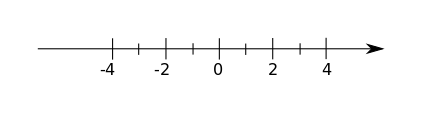
\includegraphics{images/polynomials_03.png}
\caption{Page1}
\end{figure}

Cosets are ``shifted'' ideals; e.g. \(J+1\) is the ideal shifted by one:
\(J+1 = \{\ldots,-3,-1,1,3,\ldots\}\). The set of all cosets cover the
complete \(\mathbb{Z}\). Cosets are either disjoint or contain the same
elements. In this case it is rather obvious when two cosets are disjoint
(e.g.~J and J+1) or contain the same elements (e.g.~J and J+2).

\subsection{\texorpdfstring{The Field
\(\mathbb{Z}[x] / \langle p(x) \rangle\)}{The Field \textbackslash{}mathbb\{Z\}{[}x{]} / \textbackslash{}langle p(x) \textbackslash{}rangle}}\label{the-field-mathbbzx-langle-px-rangle}

Let p(x) be a polynomial with coefficients from \(\mathbb{Z}\);
therefore the polynomial is from \(\mathbb{Z}[x]\). In the extension
field topic, \(p(x)\) has a root: \(p(\alpha) = 0\).

\(J = \langle p(x) \rangle\) is the ideal; i.e.~all polynomials of the
form \(a(x)p(x), a(x) \in \mathbb{Z}[x]\). Note that all elements of the
ideal have \emph{at least} the root \(\alpha\) (the \(a(x)\) may
introduce other roots as well).

If we choose \(p(x) = x^2-2\), then
\(J = \{ \ldots, x^2-2, x(x^2-2), (x+1)(x^2-2), \ldots \}\). Somewhat
unintuitively, \(J\) does \emph{not} contain \emph{all} polynomials of
\(\mathbb{Z}[x]\) (similar to the ideal \(\langle 2 \rangle\));
e.g.~polynomials of degree 0 and 1 are not contained in J.

A coset \(J + a\) is defined as
\(\{j + a, j \in J, a \in \mathbb{Z} \}\) for fixed \(a\) and \(j\)
ranging over the whole ideal J. Note that the cosets are disjoint sets
(i.e. \(J+a\) and \(J+b\) are disjoint for \(a \neq b\)) and partition
\(\mathbb{Z}\). In our example, the coset \(J + -(x^2-2)\) will contain
the constant polynomial \(1\). While for the cosets of the ideal
\(I = \langle 2 \rangle\) it was obvious which cosets are disjoint and
which contain the same elements, this is not obvious in this example.

The quotient ring is the set of all cosets; i.e.
\(\mathbb{Z} / \langle p(x) \rangle = \{\ldots, J - x, J-2x, J, J+x^2, J+2x^2,\ldots\}\).
This quotient ring forms a field.

%\DiaryEntry{Finite Fields, I}{2016-08-17}{Algebra}

The sets \(\mathbb{Z}_p\) with p being prime are finite fields under
modulo-p addition and modulo-p multiplication.

When p is not prime, the set is not a field because multiplication does
not have an inverse: We can factor p as \(p=qr\) with \(1< q,r < p\) and
therefore \(qr \mod p = 0\). But this means that the product of two
non-zero factors is zero; i.e.~neither q nor r have a multiplicative
inverse.

This has been easy; I'm not so sure whether a proof for the inverse is
needed: If p is prime, then there is exactely one pair of \(q,r\) with
\(1 \leq q,r < p\) for which \(qr \mod p = 1\) holds; i.e.~q is
invertible with the inverse being r. Maybe show that the product
\(qr \mod p\) takes on all possible values. There are p possible values
and therefore one and only one product must equal 1.

Anyway, continue with p being prime. Every set of the form
\(\mathbb{Z}_{p^n}\) is a (finite) field and will be denoted as
GF(\(p^n\)). These fields can be constructed as field extension to
GF(p)\$: Find an irreducible polynomial over GF(p) of order \(n\) and
construct a field extension using one of the polynomials roots. This
field is then GF(\(p^n\)).

\subsection{GF(2\^{}2)}\label{gf22}

Use the polynomial \(a(x) = x^2+x+1\) which has no roots in
\(\mathbb{Z}_2\): \(a(0) = 1, a(1) = 1\). Let us denote a root with
\(\alpha\) and we therefore have \(\alpha^2+\alpha+1=0\). We can use
this identity to construct addition and multiplication tables for
GF(\(2^2\))

\[
\begin{array}{c|cccc}
+  &       0        & 1          & \alpha     & 1+\alpha \\
\hline
0 &        0        & 1          & \alpha     & 1+\alpha \\
1 &        1        & 0          & 1 + \alpha & \alpha   \\
\alpha &   \alpha   & 1 + \alpha & 0          & 1        \\
1+\alpha & 1+\alpha & \alpha     & 1          & 0        \\
\end{array}
\]

wherer we have used the fact that \(1 + 1 = 0\) and
\(\alpha + \alpha = \alpha (1+1) = 0\). The multiplication table looks
as follows

\[
\begin{array}{c|cccc}
\times  &    0        & 1        & \alpha     & 1+\alpha \\
\hline
0 &        0        & 0        & 0          & 0 \\
1 &        0        & 1        & \alpha     & 1 + \alpha   \\
\alpha &   0        & \alpha   & 1 + \alpha & 1        \\ 
1+\alpha & 0        &1+\alpha &  1  &        \alpha      \\
\end{array}
\]

where we used the fact that \(\alpha^2 + \alpha +1 =0\). From this we
deduce \(\alpha^2=-1-\alpha = 1 + \alpha\) because \(-1 \mod 2 =1\) and
also
\((1+\alpha)^2 = 1 + 2\alpha + \alpha^2 = 1 + \alpha^2 = 1 + 1 + \alpha = \alpha\).

Taken from $2016-08-05-fieldext_01$

\subsection{GF(2\^{}3)}\label{gf23}

Use the polynomial \(a(x)=x^3+x+1\) which is irreducible over GF(2). The
elements of GF(\(2^3\)) are of the form \(a_0 + a_1 x + a_2 x^2\) with
\(a_0, a_1, a_2 \in \mathbb{Z}_2\). These are \(2^3=8\) elements.
Addition and multiplication tables are as follows:

\[
\begin{array}{c|cccccccc}
+ & 0 & 1 & \alpha & \alpha+1 & \alpha^2 & \alpha^2 + 1 & \alpha^2 + \alpha & \alpha^2 + \alpha + 1\\
\hline
0                     &       0        & 1          & \alpha     & \alpha + 1 & \alpha^2 & \alpha^2 + 1 & \alpha^2 + \alpha & \alpha^2 + \alpha + 1 \\
1                     &        1        & 0          & \alpha + 1 & \alpha   & \alpha^2 + 1 & \alpha^2 & \alpha^2 + \alpha + 1 & \alpha^2 + \alpha \\
\alpha                &   \alpha   & \alpha + 1 & 0          & 1  & \alpha^2 + \alpha & \alpha^2 + \alpha + 1 & \alpha^2 & \alpha^2 + 1 \\
\alpha+1              & \alpha + 1     & \alpha     & 1         &   0       & \alpha^2 + \alpha + 1 & \alpha^2 + \alpha &  \alpha^2 + 1 & \alpha^2 \\
\alpha^2              & \alpha^2 & \alpha^2 + 1 & \alpha^2 + \alpha & \alpha^2 + \alpha + 1 & 0 & 1 &  \alpha & \alpha + 1 \\
\alpha^2 + 1          & \alpha^2 + 1 & \alpha^2 & \alpha^2 + \alpha + 1 & \alpha^2 + \alpha & 1 & 0 & \alpha + 1 & \alpha \\
\alpha^2 + \alpha     & \alpha^2 + \alpha & \alpha^2 + \alpha + 1 & \alpha^2 & \alpha^2 + 1 & \alpha & \alpha + 1 & 0 & 1 \\
\alpha^2 + \alpha + 1 &  \alpha^2 + \alpha + 1 & \alpha^2 + \alpha & \alpha^2 + 1 & \alpha^2 & \alpha + 1 & \alpha & 1 & 0
\end{array}
\]

\[
\begin{array}{c|ccccccc}
\times                     &       1          & \alpha     & \alpha+1 & \alpha^2 & \alpha^2 + 1 & \alpha^2 + \alpha & \alpha^2 + \alpha + 1\\
\hline
1                     & 1          & \alpha     & \alpha+1 & \alpha^2 & \alpha^2 + 1 & \alpha^2 + \alpha & \alpha^2 + \alpha + 1\\
\alpha      & \alpha & \alpha^2 & \alpha^2 + \alpha & \alpha + 1 & 1 & \alpha^2 + \alpha + 1 & \alpha^2 + 1 \\
\alpha+1              & \alpha + 1 & \alpha^2 + \alpha & \alpha^2 + 1 & \alpha^2 + \alpha + 1 & \alpha^2 & 1 & \alpha \\
\alpha^2 & \alpha^2 & \alpha +1 & \alpha^2 + \alpha + 1 & \alpha^2 + \alpha & \alpha & \alpha^2+1 & 1 \\ 
\alpha^2 + 1          & \alpha^2 + 1 & 1 & \alpha^2 & \alpha & \alpha^2+\alpha +1 & \alpha + 1& \alpha^2 + \alpha \\
\alpha^2 + \alpha  & \alpha^2 + \alpha & \alpha^2 + \alpha +1 & 1 & \alpha^2+1 & \alpha + 1 & \alpha & \alpha^2 \\
\alpha^2 + \alpha + 1 & \alpha^2 + \alpha + 1 & \alpha^2 + 1 & \alpha & 1 & \alpha^2+\alpha & \alpha^2 & \alpha +1 
\end{array}
\]

%\DiaryEntry{Finite Fields, II}{2016-08-22}{Algebra}

\subsection{General}\label{general}

All GF(\(p^n\)) elements takes coefficients from \(\mathbb{Z}_p\); an
element from GF(\(p^n\)) has therefore the form

\[
\sum_{k=0}^{n-1} c_k \alpha^k, c_k \in \mathbb{Z}_p
\]

We can add and multiply these elements - however, it can happen (in case
of multiplication) that the resulting element degree is larger than
\(n\). This is nothing to worry, but we seek a method of bringing these
elements into a space with degree less than \(n\) anyway. The idea is to
use an irreducible polynomial of degree n, denoted as \(p(x)\). Because
it is irreducible, it has a root \(\alpha\) outside \(\mathbb{Z}_p\):

\[
p(\alpha) = 0
\]

This expression allows us to reduce expressions with higher degree than
\(n\): Assume that we have an GF(\(p^n\)) element \(a(\alpha)\) with
degree larger than \(n\), then we can write \[
a(\alpha) = b(\alpha) p(\alpha) + c(\alpha)
\]

where \(b(\alpha), c(\alpha)\) are uniquely defined. But we have defined
\(p(\alpha)=0\), therefore \(b(\alpha) p(\alpha) = 0\) as well. So
\(a(\alpha)\) and \(c(\alpha)\) are equivalent modulo-p(x); instead of
working with polynomial degrees larger than n we can consider working
with \(c(\alpha)\) instead.

It is important to note that the difference between different galois
fields is the irreducible polynomial;the elements always look the same,
only the polynomials \(p(x)\) differ. This is analoguous to
\(\mathbb{Z}_p\): Here we reduce large numbers (resulting from addition
and multiplication) by taking their modulo expression. The whole
construction works only if \(p\) is prime in case of \(\mathbb{Z}_p\)
(otherwise there would be no multiplicative inverse element). In a
similar spirit, the polynomial \(p(x)\) must be irreducible for the
resulting structure to be a galois field.

\subsection{Cyclic Multiplicative
Group}\label{cyclic-multiplicative-group}

Every field F contains a multiplicative group denoted by \(F^\star\). In
the examples from the previous post, this group is F without the element
0.

There is a general theorem (without proof): If G is a finite subgroup of
\(F^\star\) (the multiplicative group of nonzero elements of a field F),
then G is cyclic.

We can specialise this to: The multiplicative group of all nonzero
elements of a finite field is cyclic.

As an example, take GF(2\^{}3) with the irreducible polynomial
\(\alpha^3 + \alpha + 1\). Starting with \(\alpha\), we have the
following table:

\[
\begin{array}{cc}
\alpha^0 & 1 \\
\alpha^1 & \alpha \\
\alpha^2 & \alpha^2 \\
\alpha^3 & \alpha +1 \\
\alpha^4 & \alpha^2 + \alpha \\
\alpha^5 & \alpha^2 + \alpha + 1 \\
\alpha^6 & \alpha^2 + 1 \\
\alpha^7 & 1 \\
... & ...
\end{array}
\]

So, the element \(x\) is a generator for the field GF(2\^{}3).

%\DiaryEntry{Concurrent Events}{2016-08-24}{Stochastic}


Assume exactly two events occur in a timespan of \(T\). Each event lasts a time of \(d\). What is the probability that the two events overlap in time?

The Figure below shows the two events on the x and y axis,respectively. The shaded region is when the two events overlap.

\begin{figure}[H]
\centering
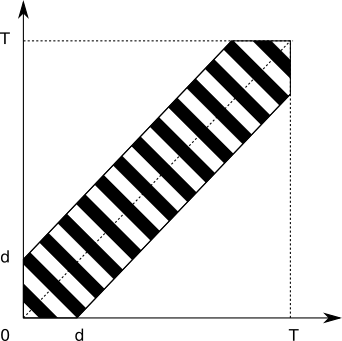
\includegraphics{images/concurrent_events.png}
\caption{Page1}
\end{figure}

In order to calculate the probability, we need to calculate areas:

The triangle below the shaded region has area \(\frac{1}{2}(T-d)^2\) and this is the same area as the triangle above. Therefore, the area of the shaded region is

\[
A = T^2 - (T-d)^2
\]

and the probability of an event overlap \(P\) is therefore

\[
P = \frac{T^2 - (T-d)^2}{T^2} = 1 - \left( \frac{T-d}{T}\right)^2
\]

In the extreme case of \(d=T\), we have \(P=1\) and for \(d=0\) we obtain \(P=0\). Both of these cases make intuitively sense.

In the case of \(d\) begin small, we can approximate \(P\) as follows

\[
P = 1 -  \frac{T^2 - 2dT + d^2}{T^2} = 1 - \left( 1 - 2\frac{d}{T} + \frac{d^2}{T^2} \right) \approx 2 \frac{d}{T}
\]

%\DiaryEntry{Lattices, I}{2016-08-30}{Algebra}


\subsection{Background}\label{background}

A relation on a set \(X\) is a subset of \(X \times X\) (i.e the subset
for which the relation holds).

\subsubsection{Partial Orderings}\label{partial-orderings}

A relation \(P\) is a partial order of \(X\), if it fulfills the
following conditions:

\begin{itemize}
\item
  It is reflexive: \((a,a) \in P, \forall a \in X\).
\item
  It is antisymmetric: If \((a,b) \in P\) and \((b,a) \in P\), then
  \(a=b\)
\item
  It is transitive: If \((a,b) \in P\) and \((b,c) \in P\), then
  \((a,c) \in P\).
\end{itemize}

Note that this definition does \textbf{not} require that all elements of
X are lreated with each other; i.e.~some elements may not be related
with each other.

If a relation is \textbf{total}, then either \((a,b) \in P\) or
\((b,a) \in P\) for \textbf{all} \(a,b \in X\) - in other words, all
elements of the set can be compared with each other.

As an example of a partial ordering, consider the power set (the set of
all subsets) of the set \(X=\{a,b,c\}\). Then the power set are the
following sets: \[
\{\}, \{a\}, \{b\},\{c\}, \{a,b\}, \{a,c\}, \{b,c\}, \{a,b,c\}
\]

Set inclusion, denoted by \(\subseteq\) is a partial ordering: For
example, we have \(\{a\} \subseteq \{a,b\}\), but there is no relation
between \(\{a\}\) and \$\{b\} or between \(\{a\}\) and \(\{b,c\}\).

These relations (and their lack between certain elements) can be
visualised in a Hasse diagram as shown below.

\begin{figure}
\centering
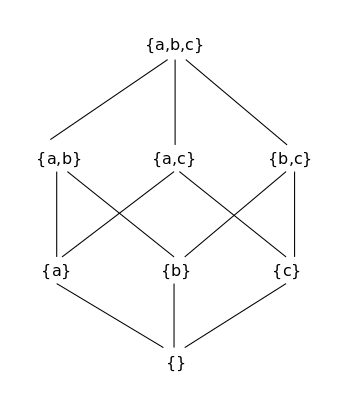
\includegraphics{images/lattices_01_1.png}
\caption{Page1}
\end{figure}

Another example is the partial order defined by \(a \leq b\) as
\(a | b\) with \(a,b \in \mathbb{N}\). This is reflexive, as \(a | a\)
holds fors all \(a,b\). If \(a|b\) and \(b|a\), then \(a=b\), so the
relation is antisymmetric, Finally, the relation is transitive, because
if \(m|n\) and \(n|p\), then \(m|p\).

If we consider the set \(X=\{1,2,3,4,6,8,12,24\}\) with this relation,
then we obtain the following Hasse diagram.

\begin{figure}
\centering
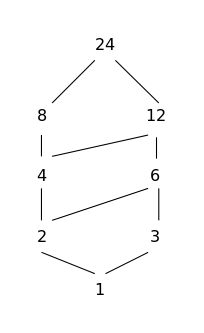
\includegraphics{images/lattices_01_2.png}
\caption{Page1}
\end{figure}

%\DiaryEntry{Splitting Fields and Finite Fields}{2016-09-05}{Algebra}

\subsection{Splitting Fields}

Let F be a field and \(p(x)\) be a polynomial over F{[}x{]}. We can find
a field extension E that contains \textbf{one} root of the polynomial.
An extension field E of F is a \textbf{splitting field} if it contains
all roots; i.e.~we can write

\[
p(x) = (x - \alpha_1)(x - \alpha_2)\cdots(x - \alpha_n)
\]

with the elements \(\alpha_i\) being in E such that
\(E = F(\alpha_1, \cdots,\alpha_n)\). A polynomial splits in E if it is
the product of linear factors in E{[}x{]}.

As an example consider \(p(x) = x^4 + 2x^2 - 8\). Over the field
\(\mathbb{Q}[x]\), the polynomial has irreducible factors \(x^2-2\) and
\(x^2+4\) with roots \(\pm \sqrt{2}, \pm 2i\). A spliting field is
\(\mathbb{Q}(\sqrt{2},i)\) as it allows an expression by means if linear
factors.

The polynomial \(x^3 - 3\) has a root in \(\mathbb{Q}(\sqrt{3})\);
however, this is \textbf{not} a splitting field as it does not contain
all roots of the polynomial which are

\[
\frac{- 3^{1/3} \pm 3^{5/6}i }{2}
\]

It can be shown that there always exists a splitting field and the
splitting field is unique.

\subsection{Finite Fields / Galois Fields}

A polynomial \(p(x)\) of degree n over a field is separable, if it has
\(n\) different roots in the splitting field of \(p(x)\); i.e.~the
polynomial factors into different linear factors.

The poylnomial \(x^2 - 2\) is separable over \(\mathbb{Q}(\sqrt{2})\) as
it contains both roots \(\pm \sqrt{2}\).

A polynomial is separable, if \(p(x)\) and \$p'(x) are relatively prime.

Proof: If a polynomial is separable, it can be written as
\(p(x) = (x-\alpha_1)(x-\alpha_2)\cdots(x-\alpha_n)\), with the
\(\alpha\) all being different. The derivative of this expresion is
\(p'(x) = (x - \alpha_2)\cdots(x-\alpha_n) + (x-\alpha_1)(x-\alpha_3)\cdots(x-\alpha_n) + \cdots\).
It can be seen that \(p(x)\) and \(p'(x)\) do not share any common
factors.

For the proof of the the opposite direction, we assume that
\(p(x) = (x-\alpha)^k g(x)\) where \(g(x)\) is another polynomial. For
the derivative, we obtain
\(p'(x) = k(x-\alpha)^{k-1} g(x) + (x-\alpha)^k g'(x)\) which have a
common factor.

In the example from above, we have \(p'(x) = 2x\) which has no common
factors with \(x^2-2\), therefore the polynmial is separable.

For every prime p and positive integer n, there exists a finite field F
with \(p^n\) elements. This field is called the Galois Field
GF(\(p^n\)). Every subfield of GF(\(p^n\)) has \(p^m\) elements, where m
divides n.

As an example consider GF(\(p^{24}\)) which therefore has subfields
GF(\(p\)), GF(\(p^2\)), GF(\(p^3\)), GF(\(p^3\)), GF(\(p^4\)),
GF(\(p^6\)), GF(\(p^8\)), and GF(\(p^{12}\)). These fields are subfields
of each other (e.g.~GF(\(p^6\)) has subfields GF(\(p\)), GF(\(p^2\)),
and GF(\(p^3\))) so in total there is a lattice of subfields.

%\DiaryEntry{Projection onto a Plane}{2017-10-04}{Maths}

Consider the following optimization problem

\[
\hat{\mathbf{x}} = \arg \min || \mathbf{y} - \mathbf{Ax} ||^2
\]

where \(\mathbf{x,\hat{x}, y}\) are \(n\)-element vectors and \(\mathbf{A}\) is an \(n \times m\) matrix. We can interpret the problem that the columns of \(\mathbf{A}\) span a vector space and we seek an ``optimal'' representation \(\hat{\mathbf{x}}\) of the vector \(\mathbf{y}\) in this space (optimum means in the least-squares sense).

We constrain the problem to the three-dimensional case; i.e. \(n=3\). If the matrix \(\mathbf{A}\) has the following form

\[
\mathbf{A} = \begin{pmatrix} 1 & 0 \\ 0 & 1 \\ 0 & 0 \end{pmatrix}
\]

then we seek a vector \(\hat{\mathbf{x}} = [\hat{x}_1, \hat{x_2}, \hat{x_3} ]^T\) which is located in the \(x-y\) plane (i.e. \(\hat{x_3}=0\)) which is closest to the vector \(\mathbf{y} = [y_1, y_2, y_3]^T\) which lies in the \(x-y-z\)-space. Therefore the result will be

\[
\hat{\mathbf{x}} = [y_1, y_2, 0]^T
\]

The follwing cvxopt/cvpy program solves this problem

\begin{verbatim}
import cvxpy as cvx
import numpy as np

x = cvx.Variable(2,1)
A = np.array([[1, 0], [0, 1], [0, 0]])
y = np.array([1,2,3])

# Form objective.
obj = cvx.Minimize(cvx.sum_entries(cvx.square(A*x - y)))

# Form and solve problem.
prob = cvx.Problem(obj)
prob.solve()  # Returns the optimal value.
print("status:", prob.status)
print("optimal value", prob.value)
print("optimal var", x.value)
\end{verbatim}

and yields

\begin{verbatim}
status: optimal
optimal value 8.99999996720797
optimal var [[ 1.] [ 2.]]
\end{verbatim}

as expected.

If we choose another matrix \(\mathbf{A}\), then we obtain another result \(\hat{\mathbf{x}}\), because the vector \(\hat{\mathbf{x}}\) represents the solution in terms of coordinates of the columns of \(\mathbf{A}\). The ``real'' answer is the product $\mathbf{A}\hat{\mathbf{x}}$.

\begin{verbatim}
import cvxpy as cvx
import numpy as np

x = cvx.Variable(2,1)
A = np.array([[2, 0], [0, 0.5], [0, 0]])
y = np.array([1,2,3])

# Form objective.
obj = cvx.Minimize(cvx.sum_entries(cvx.square(A*x - y)))

# Form and solve problem.
prob = cvx.Problem(obj)#, constraints)
prob.solve()  # Returns the optimal value.
print("status:", prob.status)
print("optimal value", prob.value)
print("optimal var", x.value)
\end{verbatim}

yields

\begin{verbatim}
status: optimal
optimal value 8.999999965622576
optimal var [[ 0.5] [ 4. ]]
\end{verbatim}

which is different than before. The product is \(\mathbf{A}\hat{\{mathbf{x}} = [1,2,0]^T\) as before.

\subsection{Additional Constraints}

We can (of course) constrain the problem; i.e.

\[
\hat{\mathbf{x}} = \arg \min || \mathbf{y} - \mathbf{Ax} ||^2 s.t. \mathbf{Bx} \leq \mathbf{c}
\]

with another \(b \times n\) matrix \(\mathbf{B}\) and length-n vector \(\mathbf{c}\). Constraining \(\mathbf{x}\) as \(x_0 \leq 0, x_1 \leq 1\) yields the solution

\[
\hat{\mathbf{x}} = [0, 1, 0]^T
\]

which can be checked with the following script

\begin{verbatim}
import cvxpy as cvx
import numpy as np

x = cvx.Variable(2,1)
A = np.array([[1, 0], [0, 1], [0, 0]])
y = np.array([1,2,3])

# Create two constraints.
constraints = [ x[0] < 0, x[1] < 1]

# Form objective.
obj = cvx.Minimize(cvx.sum_entries(cvx.square(A*x - y)))

# Form and solve problem.
prob = cvx.Problem(obj, constraints)
prob.solve()  # Returns the optimal value.
print("status:", prob.status)
print("optimal value", prob.value)
print("optimal var", x.value)
\end{verbatim}

which yields

\begin{verbatim}
status: optimal
optimal value 10.999999945179262
optimal var [[ -1.32051469e-09][  9.99999999e-01]]
\end{verbatim}

as expected.

\subsection{Minimum Distance between Point and Line}

In this case we seek the minimum distance between a point \(\mathbf{x}=[x_0, x_1]^T\) on a (given) line and a given point \(\mathbf{p} = [p_0, p_1]^T\) not located on the line. The objective is simple, we want to minimize \(||\mathbf{x} - \mathbf{p}||^2\). The constraint is a bit more tricky; we assume the line runs through the point \(\mathbf{a}\) and has a normal \(\mathbf{n}\). In this case the line equation becomes \((\mathbf{x}-\mathbf{a})^T \mathbf{n}\).

The optimization problem is therefore

\[
\hat{\mathbf{x}} = \arg \min || \mathbf{x} - \mathbf{p} ||^2, \quad s.t. (\mathbf{x}-\mathbf{a})^T \mathbf{n}
\]

and the corresponding cvxopt / cvxpy script is

\begin{verbatim}
import cvxpy as cvx

x = cvx.Variable(2,1)

# normal vector of the line
n = [1, 1]
# displacement of the line
a = [2, 0]

# the point
p = [3,2]

# Create the line constraint
constraints = [ x[0]*n[0] + x[1]*n[1] == a[0]*n[0] + a[1]*n[1]]

# Form objective.
obj = cvx.Minimize(cvx.sum_entries(cvx.square(x - p)))

# Form and solve problem.
prob = cvx.Problem(obj, constraints)
prob.solve()  # Returns the optimal value.
print("status:", prob.status)
print("optimal value", prob.value)
print("optimal var", x.value)
\end{verbatim}

yields the result

\begin{verbatim}
status: optimal
optimal value 4.499999956206729
optimal var [[ 1.49994829] [ 0.50005171]]
\end{verbatim}

We can check the result as follows: \(\hat{\mathbf{x}} = [3/2, 1/2]^T\) must lie on the line: \((\hat{\mathbf{x}} - \mathbf{a})^T \mathbf{n} = 0\) which is fulfilled. In addition, the connection between \(\mathbf{p}\) and \(\hat{\mathbf{x}}\) must be parallel to the line's normal \(\mathbf{n}\): \(\mathbf{p} - \hat{\mathbf{x}} = [3/2, 3/2]^T\) which is also fulfilled.

\subsection{Minimum Distance between Point and Circle}

We can choose another constraint; e.g.~minimize the distance between a point constrained inside a circle and a given point. We then have

\[
\hat{\mathbf{x}} = \arg \min || \mathbf{x} - \mathbf{p} ||^2, \quad s.t. || \mathbf{x}-\mathbf{a} < r||^2 < r
\]

and the corresponding cvxopt / cvxpy script is

\begin{verbatim}
import cvxpy as cvx
import numpy as np

x = cvx.Variable(2,1)

# center of the circle
a = [1, 1]

# the point
p = [3,3]

# Create the circle constraint
constraints = [ cvx.norm(x - a) < 1.]

# Form objective.
obj = cvx.Minimize(cvx.sum_entries(cvx.square(x - p)))

# Form and solve problem.
prob = cvx.Problem(obj, constraints)
prob.solve()  # Returns the optimal value.
print("status:", prob.status)
print("optimal value", prob.value)
print("optimal var", x.value)
\end{verbatim}

with result

\begin{verbatim}
status: optimal
optimal value 3.3431456296304973
optimal var [[ 1.70710683] [ 1.70710676]]
\end{verbatim}

The optimal point \(\hat{\mathbb{x}}\) lies at the right-upper 45° corner of the circle.

\subsection{The Intersection of Convex Sets is Convex}

Note that constraints are (implicitly) and-wired. So the two constraints \(|| \mathbf{x}-\mathbf{a_1} ||^2 < r^2_1, || \mathbf{x}-\mathbf{a_2}<r_2^2 ||^2\) describe the \textbf{intersection} of the two circles located at \(\mathbf{a_1}\) and \(\mathbf{a_2}\). With each constraint being convex, and the intersection being an operation preserving convexity (see below), the resulting constraint is a convex set.

A convex set \(\mathbb{C}\) is defined as follows: For two points \(P_1, P_2 \in \mathbb{C}\), all points of the form \(t P_1 + (1-t) P_2 \in \mathbb{C}, t \in [0,1]\).

Now assume we have two convex sets \(\mathbb{C}_1, \mathbb{C}_2\) and their intersection \(\mathbb{C} = \mathbb{C}_1 \cap \mathbb{C}_2\). If \(P_1, P_2 \in \mathbb{C}\), this means that the two points will be contained in both sets (that's the definition of convexity). But then any linear combination of the two points will also be contained in both sets and this is equivalent to stating that the intersection is convex.

The figure below shows an example for \(\mathbf{a}_1 = \mathbf{0}, \mathbf{a}_2 = [1,0]^T\) and \(r_1 = r_2 = 1\).

\begin{figure}
\centering
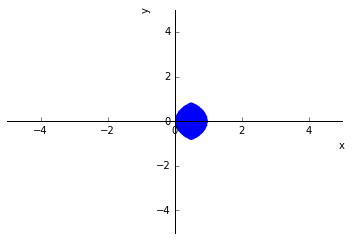
\includegraphics{images/optimization_01_1.png}
\caption{Page1}
\end{figure}

Note that the union is \textbf{not convex}: E.g. the union of
\(|| \mathbf{x}-\mathbf{0} ||^2 < 1\) and
\(|| \mathbf{x}- [2,0]^T < 1 ||^2\) is not convex.

%\DiaryEntry{Galois Theory, High-level}{2016-09-08}{Algebra}

A polynomial of degree \(n\) has \(n\) roots over \(\mathbb{C}\).

Polynomials of degree 2, 3, and 4 can be solved using expressions
involving addition/subtraction, multiplication/division, and roots (of
arbitrary) order. Such expressions are called radicals. However, finding
general expressions for polynomials of order 5 is not possible.

This does not mean that these roots do not exist (e.g.~because the field
does not contain the roots) but only that they are not expressible via
radicals. If the roots of such a polynomial are calculated by numerical
means, they do not look any different; they are just real or complex
numbers.

\subsection{Basic Idea}\label{basic-idea}

The roots of a specific polynomial can be connected via algebraic
equations. Galois Theory considers permutations of the roots; The Galois
group is the permutation group containing all permutations that leave
any algebraic equation (with rational coefficients) of the roots intact.

Iff the Galois group has the property of ``solvability'', then the
corresponding polynomial can be solved by means of radicals (otherwise
it is not possible).

As an example consider the equation

\[
x^2-4x+1
\]

with roots \(A = 2 + \sqrt{3}, B = 2 - \sqrt{3}\). Examples of algebraic
equations (with rational coefficients) the roots fulfill are


\begin{align}
A+B= & 4 \\
A \times B= &1
\end{align}


Since there are only two roots, there is only one permutation possible;
i.e. \(A \rightarrow B, B \rightarrow A\). Permuting the roots, the two
equations above are still fulfilled. It is not obvious, but the
permutation will leave \emph{any} algebraic equation with rational
coefficients intact.

The constraint of algebraic equation with rational coefficients is
important; as e.g. \(A - B - 2\sqrt{3}=0\) but which does not hold when
A and B are exchanged. However, this is not an equation with rational
coefficients, so this is ok.

%\DiaryEntry{Harmonic Series}{2016-09-12}{Maths}

\subsection{Definition}

The harmonic series is defined as

\[
H_n  = \sum_{k=1}^n \frac{1}{k}
\]

\subsubsection{Divergence}

This series diverges for \(n \rightarrow \infty\) which can be shown as follows: We have

\[
H_\infty = 1 + \frac{1}{2} + \frac{1}{3} + \frac{1}{4} + \frac{1}{5} + \frac{1}{6} + \cdots
\]

which terms we can group according to powers of 2: We put one term into group 1, 2 terms into group 2, 4 terms into group 3 etc.

\[
H_\infty = 1 + \left( \frac{1}{2} + \frac{1}{3} \right) + \left( \frac{1}{4} + \frac{1}{5} + \frac{1}{6} + \frac{1}{7} \right) +  \left( \frac{1}{8} + \frac{1}{9} + \cdots + \frac{1}{15} \right) + \cdots
\]

The two terms in group 2 are between \(1/2\) and \(1/4\), therefore the sum is between \(1/2\) and \(1\). In a similar spirit are the terms of group 3 between \(1/4\) and \(1/8\); therefore the sum is again between \(1/2\) and \(1\). This property holds in general; i.e.~group \(k\) contains the \(2^{k-1}\) elements \(\frac{1}{2^{k-1}}\) and
\(\frac{1}{2^k - 1}\) and the sum of these elements is between \(1/2\) and \(1\).

\subsubsection{Bounds}

From this grouping procedure we obtain two bounds for \(H_n\) (with \(n\) contained in group \(k\)): For an upper bound, we bound the sum of every group by \(1\); then \(H_n \leq k\). For a lower bound, we bound every sum with \(1/2\) and therefore \(H_n > k/2\). Since \(k/2\) diverges for \(k \rightarrow \infty\), also \(H_n \rightarrow \infty\).

By observing that \(k = \lfloor \log_2 n \rfloor + 1\), we can obtain a bound for \(H_n\) in terms of \(n\) as follows

\[
\frac{\lfloor \log_2 n \rfloor + 1}{2} < H_n \leq \lfloor \log_2 n \rfloor + 1
\]

An tighter bound can be obtained by considering the following Figure:

\begin{figure}
\centering
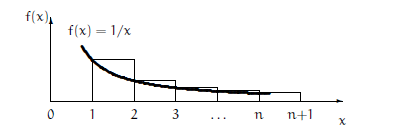
\includegraphics{images/harmonic_series_1.png}
\caption{Page1}
\end{figure}

The are below the curve between \(1\) and \(n\) is \(\int_1^n 1/x dx = \ln n\) is less than the area of the \(n\) rectangles which equals \(\sum_{k=1}^n 1/k = H_n\).

Using slightly different rectangles as shown below

\begin{figure}
\centering
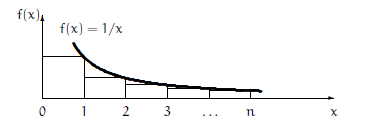
\includegraphics{images/harmonic_series_2.png}
\caption{Page1}
\end{figure}

the rectangle area \(1 + H_n\) is larger than \(\ln n\). Combining, we obtain the following bound

\[
\ln n < H_n < \ln n + 1
\]

\subsubsection{Connection with Euler's Constant}

Riemann's zeta function is defined as

\[
\zeta(r) = H_\infty^{(r)} = \sum_{k=1}^\infty \frac{1}{k^r}
\]

and converges for \(r > 1\) (Note that \(\zeta(1) = H_\infty\)).

Now consider the infinite series

\[
\ln \left( \frac{k}{k-1} \right) = \ln k - \ln(k-1) = \frac{1}{k} + \frac{1}{2k^2} + \frac{1}{3k^3} + \cdots
\]

and sum it from \(k=2...n\). The left side telescopes; i.e.~we have \(\ln 2 - \ln 1 + \ln3 - \ln 2 + \cdots + \ln n - \ln (n-1) = \ln n - \ln 1\). Therefore, we obtain

\[
\ln n - \ln 1 = \sum_{k=2}^n \left( \frac{1}{k} + \frac{1}{2k^2} + \cdots \right) = H_n-1 + \frac{1}{2} (H_n^{(2)}-1) + \frac{1}{3} (H_n^{(3)}-1) + \cdots
\]

We can rearrange this to get the different between \(H_n\) and \(\ln n\) as follows:

\[
H_n - \ln n = 1 - \frac{1}{2} (H_n^{(2)}-1) - \frac{1}{3} (H_n^{(3)}-1) - \cdots
\]

Taking the limit \(n \rightarrow \infty\), the right hand approaches the limiting value

\[
\lim_{n \rightarrow \infty} = 1 - \frac{1}{2} (\zeta(2)-1) - \frac{1}{3} (\zeta(3)-1) - \cdots = \gamma
\]

which is known as Euler's constant, \(\gamma\). Summarizing, we have

\[
\lim_{n \rightarrow \infty} = H_n - \ln n = \gamma
\]

\subsection{$H_n$ is non-integral}

Apart from \(n=1\), \(H_n\) never has an integer value. Even more, any consecutive subseries of \(H_n\), \(Smn = \frac{1}{m} + \cdots \frac{1}{n}\), is never an integer.

However, I do not understand the proof\ldots{}

\subsection{Interesting values}

Just playing around with the numbers:

\[
\begin{array}{cccc}
n & H_n & \ln n & \ln n+1 \\
\hline
1    & 1     & 0     & 1 \\
2    & 1.5   & 0.693 & 1.693 \\
5    & 2.283 & 1.609 & 2.609 \\
10   & 2.929 & 2.303 & 3.303 \\
50   & 4.499 & 3.912 & 4.912 \\
100  & 5.187 & 4.605 & 5.605 \\
1000 & 7.485 & 6.908 & 7.908
\end{array}
\]

Python:

\begin{verbatim}
% n = 1000
sum([1/x for x in range(1,1001)])
\end{verbatim}

\subsection{Application}\label{application}

Overlaying cards, as described in ``Concrete Mathematics'', Section 6.3.

%\DiaryEntry{Birthday Problem}{2016-09-16}{Maths}

The birthday problem asks for the probability that 2 (or more) persons in a room with \(r\) people share the same birthday (same day in a year). More exactly, it deals with the probability that \textbf{any} 2 (or more) persons share the same day.

If we allow \(N\) days for a year, we obtain for the probability that no people share a birthday

\[
P = \frac{N(N-1)(N-2) \cdots (N-r+1)}{N^r} = \frac{N!}{(N-r)!N^r}
\]

The first person has \(N\) possibilities, the second one has one less, etc. In total, \(r\) people can have \(N^r\) different birthdays.

The probability for ``birthday collisions'' is then

\[
P = 1 - \frac{N(N-1)(N-2) \cdots (N-r+1)}{N^r} = 1 - \frac{N!}{(N-r)!N^r}
\]

This is ``surprisingly'' high; e.g. \(P_b \approx 1/2\) for \(r=23, N = 365\) and \(P \approx 1\) for about 50 persons. The reason for this is that we are asking for \textbf{any} persons sharing birthday and there is a large number of such pairings; namely \(N(N-1)/2\) (\(N\) for the first choice, \(N-1\) for the second) which increases very quickly.

The Figure below shows the probability as function of \(r\) and \(N=365\).

\begin{figure}[H]
\centering
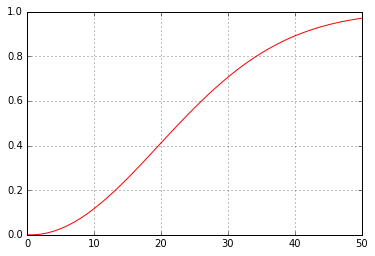
\includegraphics{images/birthday_problem_2.png}
\end{figure}

\subsection{Birthmate Problem}

Here the question is slightly different: We fix the birthday (e.g.~to the observer's birthday) and ask for the probability that one (or more) person has the same birthday.

The probability that no one has the same birthday as we is given by

\[
P = \left( \frac{N-1}{N} \right)^r
\]

Every person has the same chance of \((N-1)/N\) of not sharing birthday and we multiply this over \(r\) persons. The ``collision'' probability is then

\[
P = 1 - \left( \frac{N-1}{N} \right)^r
\]

\subsection{Discussion}

The following Figure shows plots for the birthday problem (red) and the birthmate problem (blue) as function of \(r\) and for \(N=365\).

\begin{figure}[H]
\centering
\includegraphics{images/birthday_problem_1.png}
\end{figure}

%\DiaryEntry{Cliffhanger Problem}{2016-09-20}{Stochastic}

We need to distinguish the probability of moving to the right / left \textbf{within one step} which is \(p\) / \(1-p\), respectively and the probability of absorption when started at position \(i\): \(P(abs|i)\). These latter probabilities do not consider how many steps it takes between start and absorption.

We have

\[
P(abs|1) = 1 - p + p P(abs|2)
\]

When we start at one there are two options for absorption: Move to the left directly (with probability \(1-p\)) or move to the right directly (with probability \(p\)) and being absorbed some when later (with probability \(P(abs|2)\)).

The probability for absorption starting at 2 have two parts: Going from 2 to 1 (not necessarily in one step) and going from 1 to 0 (again not necessarily in one step) with probability \(P(abs|1)\). The probability for going from 2 to 1 is the same - the only difference is that everything has been shifted to the right by one position.

Therefore, we have

\[
P(abs|2) = P(abs|1)^2
\]

and inserting this into the first equation, we obtain

\[
P(abs|1) = 1 - p + p P(abs|1)^2
\]

Solving for the absorption probability we obtain the following two solutions

\[
P(abs|1) = 1, P(abs|1) = \frac{1-p}{p}
\]

For the extreme case of \(p=0\) (no movement to the right), we will have \(P(abs|1) = 1\); i.e.~there will always be absorption. For \(p=1/2\) the two solutions yield the same value, namely \(P(abs|1) = 1\), and for the other extreme case of \(p=1\) (no movement to the left), we will have \(P(abs|1) = 0\); i.e.~no absorption.

A plot of the probability \(P(abs|1)\) for different values of \(p\) is shown in the following Figure.

\begin{figure}
\centering
\includegraphics{images/cliffhanger.png}
\end{figure}

%\DiaryEntry{Semidefinite Relaxation}{2016-09-27}{Optimization}

\subsection{Problem}

Original paper \href{\%7Bfilename\%7D/files/sdrapp-SPM.pdf}{here}, an
interesting presentation
\href{\%7Bfilename\%7D/files/20120616101847.pdf}{here}.

We want to solve the following minimization problem


\begin{align*}
\min & x^T C x \\
s.t. & x^T F_i x \geq g_i, \quad i=1,\ldots,p \\
     & x^T H_i x = l_i, \quad i=1,\ldots,m
\end{align*}


All matrices \(C, F_i, H_i\) are symmetric \(n \times n\) matrices and \(x\) is a length-n vector. This is a quadratically constrained quadratic problem (QCQP) and - in general - non-convex. As an example how the constraints may look like consider

\[ F_1 = 
\begin{pmatrix}
2 & 2 \\
2 & 3
\end{pmatrix}, F_2 = 
\begin{pmatrix}
2 & -3/2 \\
-3/2 & 3
\end{pmatrix}
\]

with \(g_1 = g_2 = 10\).

\begin{figure}[H]
\centering
\includegraphics{images/sdr_1.png}
\end{figure}

The blue region is the feasible region and is clearly not convex. The objective function has elliptical contour lines (centered at the origin) which may arbitrarily rotated with respect to the axis (depending on the matrix \(C\)).

\subsection{Solution}

We can rewrite the problem by substituting \(X = x x^T\) and obtain


\begin{align*}
\min \,\, & \text{tr} (C X) \\
s.t. & \text{tr} (F_i X) \geq g_i, \quad i=1,\ldots,p \\
     & \text{tr} (H_i X) = l_i, \quad i=1,\ldots,m \\
     & X \succeq 0, \text{rank}(X) = 1
\end{align*}


The problem has now a linear objective function, linear constraints, the psd condition on \(X\) is also not hard, but the rank-1 condition on \$X" \textbf{is} hard. This comes at no surprise as a substitution cannot convert an NP-hard problem into an easy one.

The key idea is to drop the rank-1 condition and arrive at the semidefinite relaxation


\begin{align*}
\min \,\, & \text{tr} (C X) \\
s.t. & \text{tr}(F_i X) \geq g_i, \quad i=1,\ldots,p \\
     & \text{tr}(H_i X) = l_i, \quad i=1,\ldots,m \\
     & X \succeq 0
\end{align*}


This problem is convex and can be solved with standard methods quite
easily. However, the solution will typically not be a rank-1 matrix and
the question is how to find the solution of the original problem.
According to the paper, this is ``problem-specific''; e.g.~simple
methods like an EVD of \(X\) and cutting off all eigenvalues except the
largest one, or randomization methods are mentioned.

\subsection{Example}

As an example consider solving

\begin{align*}
\min \,\, & \text{tr} (X) \\
s.t. & \text{tr}(F X) \geq 15 \\
     & X \succeq 0, \text{rank}(X) = 1
\end{align*}

with

\[
F = \begin{pmatrix} 2 & 2 \\ 2 & 3 \end{pmatrix}
\]

The constraint $\text{tr}(F X) \geq 15$ has the following form

\begin{figure}
\centering
\includegraphics{images/sdr_2.png}
\end{figure}

The contour plot of the objective function are just concentric circles with center at the origin. Wit geometric intuition, the solution of the problem is therefore the intersection of the ellipse's minor axis with the ellipse: Tis point is feasible and has minimum distance from the origin (and therefore the objective function minimal).

We can solve this with the following cvxpy script

\begin{verbatim}
import cvxpy as cvx
import numpy as np

X = cvx.Semidef(2)
F = np.array([[2, 2], [2, 3]])
constraints = [ cvx.trace(F*X) > 15]

# Form objective.
obj = cvx.Minimize(cvx.trace(X))

# Form and solve problem.
prob = cvx.Problem(obj, constraints)
prob.solve()  # Returns the optimal value.
print("status:", prob.status)
print("optimal value", prob.value)
print("optimal var", X.value)

# finding a 2-d point by using a rank-one approximation
d, u = np.linalg.eigh(X.value)
print("rank-1 approx:", np.sqrt(d[1])*u[:,1])
\end{verbatim}

which yields

\begin{verbatim}
rank-1 approx: [[ 1.11597753] [ 1.42931817]]
\end{verbatim}

Here we have used an EVD of the solution \(X\) and then take the vector corresponding to the largest eigenvalue as approximation of the original non-convex problem.

The ellipse minor axis can be found using an EVD on \(F\) which yields for the minor axis

\begin{verbatim}
array([ 0.61541221,  0.78820544])
\end{verbatim}

This is the direction of the minor axis. Let's call the slope \(\alpha = \frac{0.788\ldots}{0.615\ldots}\). The line of the minor axis in parametric form is therefore \(x = t, y = \alpha t\). The constraint is given by \(2x^2 + 3y^2 + 4xy = 15\). We seek the intersection point of line and ellipse which is obtained as

\[
2t^2 + 3\alpha^2 t^2 + 4 \alpha t^2 = 15 \rightarrow t = \sqrt{\frac{15}{2 + 4 \alpha + 3 \alpha^2}}
\]

From this value we have \(x_o =1.12, y_o = 1.43\). This value matches the result given by cvxopt (and subsequent rank-1 approximation).

%\DiaryEntry{FIR Filter Design}{2016-09-29}{Optimization}

\subsection{Problem Definition}

We want to design a linear phase filter. The filter order \(n = 2N+1\)
is odd and the impulse response is symmetric around the midpoint:

\[
h_k = H_{n-k-1}, \quad k=0,\ldots,n-1
\]

We therefore have \(h_0 = h_{n-1}, h_1 = h_{n-2} \ldots\). The
corresponding frequency response \(H(e^{j \omega}\) depends only on
\(h_0,\ldots,h_N\) and is given by

\[
H(e^{j \omega} = h_0 + h_1 e^{j\omega} + h_2 e^{j2\omega} + \cdots h_{n-1} e^{j(n-1)\omega} = e^{-jN\omega} \left( 2h_0 \cos N \omega  + 2 h_1 (N-1) \omega + \cdots + h_N \right) = e^{-jN} \tilde{H}(e^{j \omega})
\]

This shows that the filter has a linear phase; the absolute value of the
frequency response is given by \(\tilde{H}(e^{j\omega})\).

In order to obtain an optimization problem, we discretize the problem;
i.e.~we calculate \(\tilde{H}(e^{j\omega})\) at a discrete number of
points. We can then write the expression for this discretized frequency
response as

\[
\mathbf{\tilde{H}} = \mathbf{W} \mathbf{h}
\]

where the i-th row of \(\mathbf{W}\) contains the values
\([\cos(\omega_i N), \cos(\omega_i (N-1)), \ldots,1]\) and
\(\mathbf{h}\) is a column vector containing the \(N\) filter
coefficients.

\subsection{Optimization Problem}

We can now define our filter design problem such that we defne a
passband and a stopband and we seek a filter with maximal stopband
attenuation, while having a defined ripple in the passband.


\begin{align*}
\min & |\mathbf{W}_s h| \\
s.t. & \mathbf{W}_p h > \delta_1 \\
     & \mathbf{W}_p h < \delta_2 \\
\end{align*}


Here, \(\mathbf{W}_s\) and \(\mathbf{W}_p\) denote the rows of
\(\mathbf{W}\) corresponding to frequencies in the passband and
stopband, respectively, and \(\delta_1, \delta_2\) denotes the ripple in
the passband.

\subsection{Solution via CvxPy}

The following script defines and solves the optimization problem above

\begin{verbatim}
# Number of FIR coefficients (including the zeroth one).
n = 20
# passfreq.
wpass = 1.2
# passripple
pass_max = 1.1
pass_min = 0.9
# stopfreq.
wstop = 1.6

# Rule-of-thumb frequency discretization (Cheney's Approx. Theory book).
m = 15*n
w = np.mat(np.linspace(0,np.pi,m)).T
# the i-th row of A contains the values [2cos w_i N 2cos w_1 (N-1) ... 1]
A = np.cos(  np.kron(np.mat(w), np.mat(np.arange(n-1,-1,-1)))  )
# indices for splitting the frequency matrix
ind_pass = np.where(w < wpass)
ind_stop = np.where(w > wstop)
# the splitted matrices
Apass = A[ind_pass[0], :]
Astop = A[ind_stop[0], :]

# definition of optimization problem
h = cvx.Variable(n)
# objective function -> mas stopband attenuation
obj = cvx.Minimize( cvx.sum_squares( Astop * h))
# passband ripple as constraint
con = [Apass * h > pass_min, Apass * h < pass_max]

# Solve problem.
prob = cvx.Problem(obj, con)
prob.solve()

print("status:", prob.status)
print("optimal value", prob.value)
print("optimal var", h.value)

# calc. frequency response
H = A * h.value
Hpass = Apass*h.value

# and plot it...
plt.plot(w, 20*np.log10(np.abs(H)))
plt.xlabel(r'$\omega$')
plt.ylabel(r'$|H(\omega)|$ in dB')
plt.title('FIR filter freq. response magnitude')

plt.grid()
\end{verbatim}

\subsection{Example}

Using the following values: n = 20, wpass =1.2, wstop = 1.6, pass\_max =
1.1, pass\_min = 0.9 we obtainth efollowing plot of the frequency
response:

\begin{figure}[H]
\centering
\includegraphics{images/fir_design_1.png}
\end{figure}

If we decrease the gap between passband and stopband (wpass =1.5, wstop
= 1.6) and leave all other parameters unchanged, the stopband
attenuation decreases as is shown below. In other words, a sharper
filter provides less stoppband attenuation.

\begin{figure}[H]
\centering
\includegraphics{images/fir_design_2.png}
\end{figure}

If we allow more filter coefficients (in this case n = 80), then we
achieve a higher stoppband attenuation as below (even though the filter
is sharper).

\begin{figure}[H]
\centering
\includegraphics{images/fir_design_3.png}
\end{figure}

%\DiaryEntry{Non-Abelian Groups}{2016-10-19}{Algebra}

Based on
\href{http://math.stackexchange.com/questions/1971166/show-that-a-nonabelian-group-must-have-at-least-five-distinct-elements}{this}.

A group has an identity element, \(e\). Then we need two more elements
\(a, b\) with \(ab \neq ba\). Furthermore, \(a\) must not be the inverse
of \(b\), as this would prevent \(ab \neq ba\). Based on this argument,
a non-abelian group could have 5 elements which are \(1, a, b, ab, ba\).

However, 5 is a prime; and groups of prime order are cyclic, and cyclic
groups are abelian: In a cyclic group, all elements have the form
\(a^n\), with \(n \in \mathbb{Z}\). Take 2 elements
\(x = a^m, y = a^n\); then \(xy = a^{m+n} = a^{n+m} = yx\) qed.

%\DiaryEntry{Klein-4 Group}{2016-10-24}{Algebra}

\subsection{Definition}\label{definition}

The Klein-4 Group \(\mathbb{K}_4\) is defined by the following equations

\[
a^2 = b^2 = (ab)^2 = e
\]

and typically \(ab\) will be denoted as \(ab = c\). In order to write
down the Cayley table, three products are missing: \(ab, ac\) and
\(bc\).

\[
\begin{array}{c|cccc}
\star   & e     & a    & b   & c     \\
\hline
e       & e     & a    & b   & c     \\
a       & a     & e    & ?   & ?     \\
b       & b     & ?    & e   & ?     \\
c       & c     & ?    & ?   & e
\end{array}
\]

For the product \(ab\) we have two options: (i) \(ab = b\), (ii)
\(ab = c\). Option (i) does not work, as it would imply that \(a = e\)
and we already have one identity element. Therefore, \(ab = c\),
\(ac = b\) and we arrive at

\[
\begin{array}{c|cccc}
\star   & e     & a    & b   & c     \\
\hline
e       & e     & a    & b   & c     \\
a       & a     & e    & c   & b     \\
b       & b     & c    & e   & ?     \\
c       & c     & b    & ?   & e
\end{array}
\]

There is only one question mark left and the remaining identites allow
to uniquely deduce \(bc = a\). We therefore have

\[
\begin{array}{c|cccc}
\star   & e     & a    & b   & c     \\
\hline
e       & e     & a    & b   & c     \\
a       & a     & e    & c   & b     \\
b       & b     & c    & e   & a     \\
c       & c     & b    & a   & e
\end{array}
\]

\subsection{Characteristics}\label{characteristics}

\begin{itemize}
\item
  All non-identity elements have order two; i.e.
  \(x \in \mathbb{K}_4 \rightarrow x^2 = e\). In other words, the main
  diagonal of the Cayley table contains only the identity element \(e\).
\item
  The group is isomorphic to \(\mathbb{Z}_2 \oplus \mathbb{Z}_2\) and
  can be represented as the pairs \(\{(0,0), (0,1), (1,0), (1,1)\}\)
  under component-wise addition modulo-2 (\(\{0,0\}\) being the identity
  element) or as bit string \(\{00, 01, 10, 11\}\) under component-wise
  xor-operation (\(\{00\}\) being the identity element).
\item
  Another isomorphism is given by the mapping
  \(e \rightarrow 1, a \rightarrow 3, b \rightarrow 5, c \rightarrow 7\)
  under multiplication modulo-8
  (\(a b \rightarrow 3 \times 5 = 15 = 7 \mod 8\)).
\item
  The Klein-4 group is an elementary abelian group as every nontrivial
  element has prime order \(p = 2\). This is also called a Boolean
  group.
\end{itemize}

\subsection{Symmetric Difference}\label{symmetric-difference}

The symmetric difference \(A \triangle B\) of two sets A and B is the
set of elements which are in either of the sets but not in their
intersection; i.e.~it is the union of the two sets, minus their
intersection.

The Figure below illustrates the concept.

\begin{figure}
\centering
\includegraphics{images/symmetric_difference.png}
\caption{Page1}
\end{figure}

As an example, consider \(A = \{1,2,3\}\) and \(B = \{3,4\}\). Then
\(A \triangle B = \{1,2,4\}\) (it does not contain \(3\) as this element
is contained in both \(A\) and \(B\) and therefore in the intersection).

By its very definition, the symmetric difference is symmetric; i.e.
\(A \triangle B = B \triangle A\). Other cases of interest are:

\begin{itemize}
\item
  The symmetric difference of the empty set and any set is the set:
  \(\{\} \triangle A = A\).
\item
  The symmetric difference of a set with itself is the empty set
  \(A \triangle A = \{\}\).
\item
  The symmetric difference of two disjoint sets is equal their union:
  \(A \cap B = \{\} \rightarrow A \triangle B = A \cup B\).
\end{itemize}

\subsubsection{Connection to Klein-4
Group}\label{connection-to-klein-4-group}

The Klein-4 group is the group generated by the symmetric difference
\(\triangle\) as the binary operation on the subsets of a powerset of a
set with two elements. We have the following power set
\(\{\}, \{\alpha\}, \{\beta\}, \{\alpha, \beta\}\).

The empty set is the identity element of the group
(\(A \triangle \{\} = A\)) and the Cayley table looks as follows:

\[
\begin{array}{c|cccc}
\star   & \{\}     & \{\alpha \}    & \{\beta\}   & \{\alpha, \beta\}     \\
\hline
\{\}       & \{\}     & \{\alpha\}    & \{\beta\}   & \{\alpha, \beta\}     \\
\{\alpha\}       & \{\alpha\}     & \{\}    & \{\alpha, \beta\}   & \{\beta\}     \\
\{\beta\} & \{\beta\}     & \{\alpha, \beta\}    & \{\}   & \{\alpha\}     \\
\{\alpha, \beta\}       & \{\alpha, \beta\}     & \{\beta\}    & \{\alpha\}   & \{\}
\end{array}
\]

\subsubsection{Generalization}\label{generalization}

If we consider powersets of sets with more than two elements, we can -
in a way - generalize the Klein-4 Group. The Klein-4 group has the
property that \(a^2 = b^2 = c^2 = e\) and with the reasoning from above,
\(A \triangle A = \{\}\). Therefore, this property of the Klein-4 group
is kept.

The next group is based on the power set of a set with 3 elements $\alpha \beta, \gamma:$\\ $\{\}, \{\alpha\}, \{\beta\}, \{\gamma\}, \{\alpha, \beta\}, \{\alpha, \gamma\}, \{\beta, \gamma\}, \{\alpha, \beta, \gamma\}$.

%\DiaryEntry{Groups of Order 4}{2016-10-25}{Algebra}

Let us find all groups with order 4. These groups must be abelian (see
\href{\%7Bfilename\%7D2016-10-19_non_abelian_group_order.markdown}{this
post} and
\href{http://math.stackexchange.com/questions/300393/group-tables-for-a-group-of-four-elements}{here}).

The first group is \(\mathbb{Z}_4\) with modulo-4 addition. Using
\(0 \rightarrow e,1 \rightarrow a,2 \rightarrow b,3 \rightarrow c\) as
group elements we have

\[
\begin{array}{c|cccc}
\star   & e     & a    & b   & c     \\
\hline
e       & e     & a    & b   & c     \\
a       & a     & b    & c   & e     \\
b       & b     & c    & e   & a     \\
c       & c     & e    & a   & b
\end{array}
\]

This group is cyclic; the sequence \(e-a-b-c\) is repeated in every row
(albeit shifted).

Another option is to start like this

\[
\begin{array}{c|cccc}
\star   & e     & a    & b   & c     \\
\hline
e       & e     & a    & b   & c     \\
a       & a     & c    & b   & e     \\
b       & b     & b    & ?   & ?     \\
c       & c     & e    & ?   & ?
\end{array}
\]

but this is not a group (3rd row).

Let's start anew

\[
\begin{array}{c|cccc}
\star   & e     & a    & b   & c     \\
\hline
e       & e     & a    & b   & c     \\
a       & a     & e    & c   & b     \\
b       & b     & c    & ?   & ?     \\
c       & c     & b    & ?   & ?
\end{array}
\]

This should work; Now we have 3 places left to fill: \(bb, bc\), and
\(cc\). Let's go as below

\[
\begin{array}{c|cccc}
\star   & e     & a    & b   & c     \\
\hline
e       & e     & a    & b   & c     \\
a       & a     & e    & c   & b     \\
b       & b     & c    & e   & a     \\
c       & c     & b    & a   & e
\end{array}
\]

which is the Klein-4 Group. The Klein-4 group is actually defined by
\(a^2 = b^2 = (ab)^2 = e\). This does not directly define \(ab\);
however, there are only 2 options: (i) \(ab = c\) or (ii) \(ab = b\). It
immediately follows that \(ab=c\) which uniquely defines the group.

However, this is not the only option, we can also fill the question
marks above like this

\[
\begin{array}{c|cccc}
\star   & e     & a    & b   & c     \\
\hline
e       & e     & a    & b   & c     \\
a       & a     & e    & c   & b     \\
b       & b     & c    & a   & e     \\
c       & c     & b    & e   & a
\end{array}
\]

This look different, but is an isomorphism of the \(\mathbb{Z}_4\)
group: We exchange column 2 and column 3 and row 2 and 3 to obtain

\[
\begin{array}{c|cccc}
\star   & e     & b    & a   & c     \\
\hline
e       & e     & b    & a   & c     \\
b       & b     & a    & c   & e     \\
a       & a     & c    & e   & b     \\
c       & c     & e    & b   & a
\end{array}
\]

We see again the cyclic behaviour of the sequence \(e-b-a-c\); if we
substitute \(b \rightarrow a, a \rightarrow b\) we obtain the original
\(\mathbb{Z}_4\) group from above:

\[
\begin{array}{c|cccc}
\star   & e     & a    & b   & c     \\
\hline
e       & e     & a    & b   & c     \\
a       & a     & b    & c   & e     \\
b       & b     & c    & e   & a     \\
c       & c     & e    & a   & b
\end{array}
\]

%\DiaryEntry{Groups - Subgroups}{2016-10-27}{Algebra}

For the definition of a subgroup, see
\href{\%7Bfilename\%7D2016-03-02_-groups_01.markdown}{this post}.

\subsection{Words}\label{words}

Let X be a subset of a group G. An expression of the form (the product
being the group operation)

\[
g = x_1^{m_1} x_2^{m_2} \cdots x_n^{m_n}
\]

with the \(m_i\) being integers and \(x_iu \in X\) is called a word in
the elements of X. The collection of all words is a subgroup of G:

\begin{itemize}
\item
  the product of two words is again a word in X.
\item
  the identity element can be expressed as word with all \(m_i = 0\).
\end{itemize}

If the collection of all words fills out G, then X is a set of
generators for G.

\paragraph{Example.}

For the Klein-4 Group, \(X = \{a,b\}\) is a set of generators as all 4
elements of the Klein-4 Group can be expressed by means of \(a\) and
\(b\): \(a^2 = e\), \(ab = c\).

\subsection{Subgroup Theorems}\label{subgroup-theorems}

A non-empty subset H of a group G is a subgroup of G if and only if
\(xy^{-1}\) belongs to H whenever \(x,y \in H\).

Proof: If \(x, y \in H \rightarrow y^{-1} \in H\) and therefore
\(x y^{-1} \in H\). If H is non-empty, \(x y^{-1} \in H\), and
\(x,y \in H\), then
\(e = x x^{-1} \in H \rightarrow x^{-1} = ex^{-1} \in H\). Finally, if
\(y \in H\), then \(y^{-1} \in H\) and therefore
\(xy = x (y^{-1})^{-1} \in H\). Therefore, H is a subgroup of G.

The intersection of two subgroups H and K of a group G is again a
subgroup.

Proof: Assume \(x,y \in H \cap K\). Then \(xy^{-1} \in H \cap K\) and
with the theorem above, $H \cap K$ is also a subgroup.

Every subgroup of \(\mathbb{Z}\) is cyclic. More generally, every
subgroup of a cyclic group is also cyclic.

%\DiaryEntry{Groupd - Symmetric Groups}{2016-10-27}{Algebra}

\subsection{Cycles}\label{cycles}

An important observation is that every permutation can be described as
product of disjoint cycles. Disjoint cycles are commutative; i.e.
\(\alpha \beta = \beta \alpha\) if \(\alpha\) and \(\beta\) are disjoint
cycles.

Every cycle of length \textgreater{} 2 can be written as product of
length-2 cycles (transpositions). We have

\begin{equation}
\label{eq:exp}
(a_1 a_2 \ldots a_k) = (a_1 a_k) \ldots (a_1 a_3)(a_1 a_2)
\end{equation}

This decomposition is not necessarily unique.

As every element of the symmetric group can be written as group of
disjoint cycles and every cycle can be written as product of
transpositions, every element of the symmetric group can be written as
product of transpositions.

\subsubsection{Inverse}\label{inverse}

The inverse of a permutation is again a permutation (otherwise we won't
have a group). If a permutation is given in term of its cycles, the
inverse is obtained by reversing the elements in each cycle; e.g.

\[
\alpha = (123)(45) \rightarrow \alpha^{-1} = (321)(54)
\]

\subsection{Transpositions}\label{transpositions}

A transposition of two arbitrary elements (a, b) can also be rewritten
as

\begin{equation}
\label{eq:transp}
(a b) = (1 a)(1 b)(1 a)
\end{equation}

We have \((1 a)(1 b)(1 a)a = (1 a)(1 b) 1 = (1 a)b = b\) and
\((1 a)(1 b)(1 a)b = (1 a)(1 b)b = (1 a)1 = a\) and finally
\((1 a)(1 b)(1 a)1 = (1 a)(1 b)a = (1 a)a = 1\).

The inverse element is \((ba)\) and can be expressed as follows

\[
(ab)^{-1} = (ba) = (1a)(1b)(1a) = (ab)
\]

By using this decomposition, we can generate any transposition and
therefore any element of \(S_n\). Therefore, the transpositions
\((1 2),(1 3), \ldots, (1 n)\) generate \(S_n\).

A given element of \(S-n\) can be written as product of transpositions
in many different ways. However, the number of transpositions which
occur is either always even or always odd.

\subsubsection{Further Identities}\label{further-identities}

We have

\[
(abc) = (ac)(ab)
\]

and we can specialize \eqref{eq:exp} to \(n=3\) with \(a_1 = 1\) to

\begin{equation}
\label{eq:exp3}
(1ba) = (1a)(1b)
\end{equation}

\subsubsection{Sign of Permutations}\label{sign-of-permutations}

We define a polynomial as

\[
P(x_1,x_2,\ldots,x_n) = \prod_{1 \leq i,j \leq n, i < j} (x_i - x_j)
\]

For a permutation \(\alpha \in S_n\), we define

\[
\alpha P = \prod_{1 \leq i,j \leq n, i < j} (x_{\alpha(i)} - x_{\alpha(j)})
\]

Example: Consider \(n = 3\) and \(\alpha = (132)\). Then we have

\[
P(x_1, x_2, x_3) = (x_1 - x_2)(x_1 - x_3)(x_2 - x_3)
\]

and (since the permutation does the following transformation:
\(1 \rightarrow 3, 2 \rightarrow 1, 3 \rightarrow 2\)):

\[
\alpha P(x_1, x_2, x_3) = (x_3 - x_1)(x_3 - x_2)(x_1 - x_2) = + P
\]

In general, \(\alpha P\) just permutes the terms of P and changes the
sign of some of them. Therefore, \(\alpha P = \pm P\); and this defines
the sign of the permutation: If \(\alpha P = P\), the sign is positive,
if \(\alpha P = -P\), the sign is negative.

Consider two permutations \(\alpha, \beta \in S_n\). Then the sign of
their product \(\alpha \beta\) is the product of the signs of \(\alpha\)
and \(\beta\).

The sign of the transposition \((12)\) is always \(-1\):
\(P(x_1, x_2) = x_1 - x_2\) and \(\alpha = (12)\), then
\(\alpha P = x_2 - x_1 = -P\). From \eqref{eq:transp}, the general
transposition \((ab)\) can be written as product of three terms,
\((a b) = (1 a)(1 b)(1 a)\) and therefore the sign of a general
transposition \((ab)\) is negative.

If a permutation contains an even number of transpositions, its sign is
+1 and it is called an even permutation; if a permutation contains an
odd number of transpositions, its sign is -1 and it is called an odd
permutation.

Since \((a_1 a_2 \ldots a_k) = (a_1 a_k) \ldots (a_1 a_3)(a_1 a_2)\), a
cycle has a positive sign if its length is odd.

\subsection{Alternating Subgroup}\label{alternating-subgroup}

The even permutations of \(S_n\) form a subgroup \(A_n\) with \(n!/2\)
elements which is called the alternating subgroup.

Proof: If \(\alpha, \beta \in A_n\), then each permutation is composed
of an even number of transpositions. The combination \(\alpha \beta\) is
then the combination of two even numbers of transpositions and therefore
also even. Writing the transposition product of \(\alpha\) in reverse
order yields \(\alpha^{-1}\) which is therefore also even. Finally, the
identity element can be obtained by combining the same transpositions;
i.e. \(e = (ab)(ab)\). Each transposition has odd sign, therefore the
sign of the prodcut of two transpositions (and therefore the identity
element) is even. \(\square\)

For \(n \geq 3\), the 3-cycles generate \(A_n\).

Proof: A 3-cycle is an even permutation: \((abc) = (ac)(ab)\), every
transposition is negative and the product of two negative signs is
positive. Both transpositions can be written in the form \((1x)\) to
obtain \((abc) = (ac)(ab) = (1a)(1c)(1b)(1a)(1b)(1a)\). Now we can
collect consecutive transposition pairs into 3-cycles (cf.
\eqref{eq:exp3}) and obtain \((abc) = (1ca)(1ab)(1ab)\) \(\square\).

\subsubsection{\texorpdfstring{Example
\(A_4\)}{Example A\_4}}\label{example-a_4}

The \(4! / 2 = 12\) elements of \(A_4\) are as follows (I have no idea
how to obtain this list :-( ):

\[
\begin{array}{cccc}
e, & (12)(34), &  (13)(24), &(14)(23) \\
(123), & (124), & (134), & (234) \\
(132), & (142), & (143), & (243)
\end{array}
\]

The product of transpositions in the first row can be rewritten as
product of 3-cycles; e.g.

\[
(12)(34) = (12)(13)(14)(13) = (132)(134)
\]

The remaining 6 odd permutations of \(S_4\) are given by

\[
\begin{array}{cccc}
(12), (13), & (14), (23), & (24), (34) \\
(1234), & (1243), & (1324)  \\
(1432), & (1342), & (1423)
\end{array}
\]

These must contain all transpositions (as they all have negative sign)
and then ``other'' permutations. The ``others'' are single cycles with
even length (have negative sign), or a product of several cycles with an
odd number of cycles having negative sign; i.e.~even length (so that the
overall sign is negative). It seem that for \(S_4\), transpositions and
length-4 cycles are enough to generate all odd permutations. Maybe this
is different for other symmetric groups.

\subsection{Using GAP}\label{using-gap}

Another tool required for the job\ldots{}

Anyway, with \href{\%7Bfilename\%7D/files/symmetric_group.g}{this
script} we can create the group \(S_4\) and list its elements using gap
as follows

\begin{verbatim}
s4:=SymmetricGroup(4);
Elements(s4);

[ (), (3,4), (2,3), (2,3,4), (2,4,3), (2,4), (1,2), (1,2)(3,4), (1,2,3), (1,2,3,4), (1,2,4,3), 
(1,2,4), (1,3,2), (1,3,4,2), (1,3), (1,3,4), (1,3)(2,4), (1,3,2,4), (1,4,3,2), (1,4,2), 
(1,4,3), (1,4), (1,4,2,3), (1,4)(2,3) ]
\end{verbatim}

From this we can deduce that \(S_4\) has the following elements:

\begin{itemize}

\item
  6 elements containing one transposition and 2 fixed points (e.g.
  \((1,2)\))
\item
  3 double transpositions (e.g. \((1,2)(3,4)\))
\item
  8 elements containing one 3-cycle and one fixed point (e.g.
  \((1,2,3)\))
\item
  6 elements containing one 4-cycle and no fixed point (e.g.
  \((1,2,3,4)\))
\end{itemize}

We can create the alternating subgroup \(A_4\) as follows

\begin{verbatim}
a4:=DerivedSubgroup(s4);
Elements(a4);

[ (), (2,3,4), (2,4,3), (1,2)(3,4), (1,2,3), (1,2,4), (1,3,2), (1,3,4), (1,3)(2,4), (1,4,2), 
(1,4,3), (1,4)(2,3) ]
\end{verbatim}

which matches the list from above.

\subsubsection{Multiplication Table of $A_4$}

The following multiplication table for \(A_4\) is created by GAP. Be
careful, the order is ``colum \(\times\) row''; e.g.~applying
\((2,4,3)\) before \((1,2,3)\) is written as \((1,2,3)(2,4,3)\) and
equals \((1,2,4)\) and \textbf{not} \((1,4,3)\).

\[
\begin{array}{c|cccccccccccc}
\star &  () & (2,3,4) & (2,4,3) & (1,2)(3,4) & (1,2,3) & (1,2,4) & (1,3,2) & (1,3,4) & (1,3)(2,4) & (1,4,2) & (1,4,3) & (1,4)(2,3) \\
\hline
() & () & (2,3,4)& (2,4,3)& (1,2)(3,4)& (1,2,3)& (1,2,4)& (1,3,2)& (1,3,4)& (1,3)(2,4)& (1,4,2)& 
(1,4,3)& (1,4)(2,3)\\
(2,3,4) & (2,3,4)& (2,4,3)& ()& (1,2,4)& (1,2)(3,4)& (1,2,3)& (1,3,4)& (1,3)(2,4)& (1,3,2)& (1,4)(2,3)& 
(1,4,2)& (1,4,3) \\
(2,4,3) & (2,4,3)& ()& (2,3,4)& (1,2,3)& (1,2,4)& (1,2)(3,4)& (1,3)(2,4)& (1,3,2)& (1,3,4)& (1,4,3)& (1,4)
(2,3)& (1,4,2)\\
(1,2)(3,4) & (1,2)(3,4)& (1,3,2)& (1,4,2)& ()& (1,3,4)& (1,4,3)& (2,3,4)& (1,2,3)& (1,4)(2,3)& (2,4,3)& 
(1,2,4)& (1,3)(2,4)\\
(1,2,3) & (1,2,3)& (1,3)(2,4)& (1,4,3)& (2,4,3)& (1,3,2)& (1,4)(2,3)& ()& (1,2,4)& (1,4,2)& (2,3,4)& (1,2)
(3,4)& (1,3,4)\\ 
(1,2,4) & (1,2,4)& (1,3,4)& (1,4)(2,3)& (2,3,4)& (1,3)(2,4)& (1,4,2)& (2,4,3)& (1,2)(3,4)& (1,4,3)& ()& 
(1,2,3)& (1,3,2)\\
(1,3,2) & (1,3,2)& (1,4,2)& (1,2)(3,4)& (1,4,3)& ()& (1,3,4)& (1,2,3)& (1,4)(2,3)& (2,3,4)& (1,3)(2,4)& 
(2,4,3)& (1,2,4)\\ 
(1,3,4) & (1,3,4)& (1,4)(2,3)& (1,2,4)& (1,4,2)& (2,3,4)& (1,3)(2,4)& (1,2)(3,4)& (1,4,3)& (2,4,3)& 
(1,3,2)& ()& (1,2,3)\\
(1,3)(2,4) & (1,3)(2,4)& (1,4,3)& (1,2,3)& (1,4)(2,3)& (2,4,3)& (1,3,2)& (1,2,4)& (1,4,2)& ()& (1,3,4)& 
(2,3,4)& (1,2)(3,4)\\
(1,4,2) & (1,4,2)& (1,2)(3,4)& (1,3,2)& (1,3,4)& (1,4,3)& ()& (1,4)(2,3)& (2,3,4)& (1,2,3)& (1,2,4)& (1,3)
(2,4)& (2,4,3)\\
(1,4,3)& (1,4,3)& (1,2,3)& (1,3)(2,4)& (1,3,2)& (1,4)(2,3)& (2,4,3)& (1,4,2)& ()& (1,2,4)& (1,2)(3,4)& 
(1,3,4)& (2,3,4)\\
(1,4)(2,3)& (1,4)(2,3)& (1,2,4)& (1,3,4)& (1,3)(2,4)& (1,4,2)& (2,3,4)& (1,4,3)& (2,4,3)& (1,2)(3,4)& 
(1,2,3)& (1,3,2)& ()
\end{array}
\]

\subsubsection{\texorpdfstring{Subgroups of
\(S_4\)}{Subgroups of S\_4}}\label{subgroups-of-s_4}

Can be listed like this

\begin{verbatim}
AllSubgroups(s4);

[ Group(()), Group([ (1,2)(3,4) ]), Group([ (1,3)(2,4) ]), Group([ (1,4)(2,3) ]), 
Group([ (3,4) ]), Group([ (2,3) ]), Group([ (2,4) ]), Group([ (1,2) ]), Group([ (1,3) ]), 
Group([ (1,4) ]), Group([ (2,4,3) ]), Group([ (1,3,2) ]), Group([ (1,4,2) ]), 
Group([ (1,4,3) ]), Group([ (1,4)(2,3), (1,3)(2,4) ]), Group([ (3,4), (1,2)(3,4) ]), 
Group([ (1,4), (1,4)(2,3) ]), Group([ (2,4), (1,3)(2,4) ]), Group([ (1,3,2,4), (1,2)(3,4) ]), 
Group([ (1,4,3,2), (1,3)(2,4) ]), Group([ (1,2,4,3), (1,4)(2,3) ]), Group([ (3,4), (2,4,3) ]), 
Group([ (1,4), (1,4,3) ]), Group([ (2,3), (1,3,2) ]), Group([ (1,2), (1,4,2) ]), Group([ (1,4)(2,3), (1,3)(2,4),
(3,4) ]), Group([ (1,2)(3,4), (1,3)(2,4), (1,4) ]), Group([ (1,2)(3,4), (1,4)(2,3), (2,4) ]), Group([ (1,4)(2,3),
(1,3)(2,4), (2,4,3) ]), Group([ (1,4)(2,3), (1,3)(2,4), (2,4,3), (3,4) ]) ]
\end{verbatim}

This may not be so meaningful; listing the elements of each group brings
more information. We can do this with this script:

\begin{verbatim}
sbgps:=AllSubgroups(s4);
for e1 in sbgps do
    Print(e1, " -> ", Elements(e1), StructureDescription(e1), "\n");
od;
\end{verbatim}

and obtain the following (comments and structure added manually).
According to the Lagrange Theorem, the subgroup order must divide 24
(the order of \(S_4\)), therefore, there must be subgroups of order
\(1,2,3,4,6,8,12,24\).

\paragraph{Trivial subgroup}\label{trivial-subgroup}

\begin{verbatim}
Group( () ) -> [ () ]
\end{verbatim}

\paragraph{Subgroups with 2 elements}\label{subgroups-with-2-elements}

These groups are isomorphic to the cyclic group \(\mathbb{Z}_2\).
Principle: Every transposition is its own inverse.

\begin{verbatim}
Group( [ (1,2)(3,4) ] ) -> [ (), (1,2)(3,4) ]
Group( [ (1,3)(2,4) ] ) -> [ (), (1,3)(2,4) ]
Group( [ (1,4)(2,3) ] ) -> [ (), (1,4)(2,3) ]
Group( [ (3,4) ] ) -> [ (), (3,4) ]
Group( [ (2,3) ] ) -> [ (), (2,3) ]
Group( [ (2,4) ] ) -> [ (), (2,4) ]
Group( [ (1,2) ] ) -> [ (), (1,2) ]
Group( [ (1,3) ] ) -> [ (), (1,3) ]
Group( [ (1,4) ] ) -> [ (), (1,4) ]
\end{verbatim}

\paragraph{Subgroups with 3 elements}\label{subgroups-with-3-elements}

These groups are isomorphic to the cyclic group \(\mathbb{Z}_3\).
Principle: \((2,3,4)^2 = (2,4,3)\) and \((2,3,4)^3 = ()\).

\begin{verbatim}
Group( [ (2,4,3) ] ) -> [ (), (2,3,4), (2,4,3) ]
Group( [ (1,3,2) ] ) -> [ (), (1,2,3), (1,3,2) ]
Group( [ (1,4,2) ] ) -> [ (), (1,2,4), (1,4,2) ]
Group( [ (1,4,3) ] ) -> [ (), (1,3,4), (1,4,3) ]
\end{verbatim}

\paragraph{Subgroups with 4 elements}\label{subgroups-with-4-elements}

The first 4 subgroups are isomorphic to
\(\mathbb{Z}_2 \times \mathbb{Z}_2\) and this is equivalent to the
Klein-4 group.

\begin{verbatim}
Group( [ (1,4)(2,3), (1,3)(2,4) ] ) -> [ (), (1,2)(3,4), (1,3)(2,4), (1,4)(2,3) ]
Group( [ (3,4), (1,2)(3,4) ] ) -> [ (), (3,4), (1,2), (1,2)(3,4) ]
Group( [ (1,4), (1,4)(2,3) ] ) -> [ (), (2,3), (1,4), (1,4)(2,3) ]
Group( [ (2,4), (1,3)(2,4) ] ) -> [ (), (2,4), (1,3), (1,3)(2,4) ]
\end{verbatim}

The next 3 subgroups are isomorphic to \(\mathbb{Z}_4\).

\begin{verbatim}
Group( [ (1,3,2,4), (1,2)(3,4) ] ) -> [ (), (1,2)(3,4), (1,3,2,4), (1,4,2,3) ]
Group( [ (1,4,3,2), (1,3)(2,4) ] ) -> [ (), (1,2,3,4), (1,3)(2,4), (1,4,3,2) ]
Group( [ (1,2,4,3), (1,4)(2,3) ] ) -> [ (), (1,2,4,3), (1,3,4,2), (1,4)(2,3) ]
\end{verbatim}

\paragraph{Subgroups with 6 elements}\label{subgroups-with-6-elements}

These subgroups are isomorphic to \(S_3\).

\begin{verbatim}
Group( [ (3,4), (2,4,3) ] ) -> [ (), (3,4), (2,3), (2,3,4), (2,4,3), (2,4) ]
Group( [ (1,4), (1,4,3) ] ) -> [ (), (3,4), (1,3), (1,3,4), (1,4,3), (1,4) ]
Group( [ (2,3), (1,3,2) ] ) -> [ (), (2,3), (1,2), (1,2,3), (1,3,2), (1,3) ]
Group( [ (1,2), (1,4,2) ] ) -> [ (), (2,4), (1,2), (1,2,4), (1,4,2), (1,4) ]
\end{verbatim}

\paragraph{Subgroups with 8 elements}\label{subgroups-with-8-elements}

These subgroups are isomorphic to \(D_8\), the diheadral group of order
8.

\begin{verbatim}
Group( [ (1,4)(2,3), (1,3)(2,4), (3,4) ] ) -> [ (), (3,4), (1,2), (1,2)(3,4), (1,3)(2,4), (1,3,2,4), (1,4,2,3), (1,4)(2,3) ]
Group( [ (1,2)(3,4), (1,3)(2,4), (1,4) ] ) -> [ (), (2,3), (1,2)(3,4), (1,2,4,3), (1,3,4,2), (1,3)(2,4), (1,4), (1,4)(2,3) ]
Group( [ (1,2)(3,4), (1,4)(2,3), (2,4) ] ) -> [ (), (2,4), (1,2)(3,4), (1,2,3,4), (1,3), (1,3)(2,4), (1,4,3,2), (1,4)(2,3) ]
\end{verbatim}

\paragraph{Subgroup with 12 elements}\label{subgroup-with-12-elements}

This is the alternating group \(A_4\).

\begin{verbatim}
Group( [ (1,4)(2,3), (1,3)(2,4), (2,4,3) ] ) -> [ (), (2,3,4), (2,4,3), (1,2)(3,4), (1,2,3), (1,2,4), (1,3,2), (1,3,4), (1,3)(2,4), (1,4,2), (1,4,3), (1,4)(2,3) ]
\end{verbatim}

\paragraph{Subgroup with 24 elements}\label{subgroup-with-24-elements}

Finally, the symmetric group \(S_4\) itself.

\begin{verbatim}
Group( [ (1,4)(2,3), (1,3)(2,4), (2,4,3), (3,4) ] ) -> [ (), (3,4), (2,3), (2,3,4), (2,4,3), (2,4), (1,2), (1,2)(3,4), (1,2,3), (1,2,3,4), (1,2,4,3), (1,2,4), (1,3,2), (1,3,4,2), (1,3), (1,3,4), (1,3)(2,4), (1,3,2,4), (1,4,3,2), (1,4,2), (1,4,3), (1,4), (1,4,2,3), (1,4)(2,3) ]
\end{verbatim}

%\DiaryEntry{Conjugacy}{2016-11-21}{Algebra}

\subsection{Definition}\label{definition}

Two elements \(x,y\) of a group G are conjugate if

\[
gxg^{-1} = y
\]

for some \(g \in G\). We first note that the definition is symmetric;
i.e when x is conjugate to y then y is conjugate to x (simply by
left-multiplying with \(g^{-1}\), right-multiplying with g, and
substituting \(g \rightarrow g^{-1}\):

\[
gxg^{-1} = y \leftrightarrow x = gyg^{-1}
\]

If we vary g, then we obtain a set of y's which are collected in the
conjugacy class of x:

\[
C(x) = \{y = gxg^{-1} | g \in G\}
\]

If the group G is abelian, the conjugcy classes are boring as we can
rewrite the definition to obtain

\[
C(x) = \{y = xgg^{-1} | g \in G\} = \{x\}
\]

Let the subset \(\mathbb{G}\) of \(G \times G\) consist of all paris
\((x,y)\) of which are conjugate to each other. Each element is
conjugate to itself because \(exe^{-1} = x\). Furthermore, if x and y
are conjugate and y and z are conjugate

\[
g_1 x g_1^{-1} = y, g_2 y g_2^{-1} = z
\]

then x and z are also conjugate. Consider \(g_2 g_1 x (g_2 g_1)^{-1}\)
which can be rewritten as

\[
g_2 g_1 x g_1^{-1} g_2^{-1} = g_2 y g_2^{-1} = z
\]

These characterisitcs define the set \(\mathbb{G}\) as an equivalence
relation and therefore the conjugcy classes partition G.

\subsubsection{Conjugacy Classes of the Dihedral
Group}\label{conjugacy-classes-of-the-dihedral-group}

The dihedral group \(D_n\) is defined in
\href{\%7Bfilename\%7D/2016-03-15-groups_04.markdown}{this post} by the
following equations:


\begin{align*}
r^n &= 1 \\
s^2 &= 1 \\
srs &= r^{-1}
\end{align*}


Let us first calculate the conjugacy class of \(r^\alpha\): We have
\(gr^\alpha g^{-1}\) and if we choose \(g = r^\beta\), we obtain
\(g^{-1} = r^{n-\beta}\) and therefore
\(y = gxg^{-1} = r^\beta r^\alpha r^{n-\beta} = r\alpha\). Choosing
\(g = s\), we have \(g^{-1} = s\) and
\(y = sg^\alpha s = r^{n - \alpha}\). Finally choosing
\(g = r^\beta s\), we have
\(y = r^\beta s r^\alpha (r^\beta s)^{-1} = r^\beta (s r^\alpha s) r^{-\beta} = r^\beta r^{n - \alpha} r^{n-\beta} = r^{n - \alpha}\).
So, the conjugacy class of \(r^\alpha\) is \(r^{n-\alpha}\).

Continuing in this fashion yields the following conjugacy classes


\begin{align*}
& \{e\}, \{r, r^{n-1}\}, \{r^2, r^{n-2}\}, \ldots \\
& \{s, r^2s, r^4s,\ldots\}, \{rs, r^3s, \ldots\}
\end{align*}


\subsubsection{Conjugacy Classes of the Symmetric
Group}\label{conjugacy-classes-of-the-symmetric-group}

Two elements of \(S_n\) have the same cycle structure if when they are
composed as products of disjoint cyclic permutations, they have the same
number of 2-cycles, 3-cycles etc.

Permutations which have the same cycle structure are conjugate in
\(S_n\). We can show this as follows: Assume that \(a,b \in S_n\) have
the same cycle structure and write the cycle decomposition of \(b\)
below the one of \(a\) (in order of decreasing cycle length and
including cycles of length 1). Now define \(g\) to be a permutation
which sends an element of \(a\) to an element in \(b\) directly below.
Then \(gbg^{-1} = a\) because moving down from an element \(a\) to an
element \(b\) (that's the effect of \(g\)), moving one to the right
(that's the effect of \(b\)), and moving back up (that's the effect of
\(g^{-1}\)) is the same as moving one to the right (that's the effect of
\(a\)).

As an example in \(S_9\) take \(a = (2539)(67)(14)\) and
\(b = (5467)(12)(38)\). Both contain a length-4 cycle and two length-2
cycles. Writing them down with the rules as above, we have


\begin{align*}
&(2539)(67)(14)(8) \\
&(5467)(12)(38)(9)
\end{align*}


Therefore, g becomes \(g=(254897)(361)\). The element g is not unique;
e.g.~rewriting \(a\) as \(a=(2539)(14)(67)(8)\) yields


\begin{align*}
&(2539)(14)(67)(8) \\
&(5467)(12)(38)(9)
\end{align*}


and \(g=(254)(36)(789)\).

It is not only that permutations with the same cycle structure are
conjugate in \(S_n\), but also that conjugate permutations have the same
cycle structure.

\paragraph{Using GAP}\label{using-gap}

We can use GAP to list conjugacy classes. In
\href{\%7Bfilename\%7D/files/conjugacy.g}{this script} we use GAP to
list all conjugacy classes of the symmetric group \(S_4\).

\begin{verbatim}
g := SymmetricGroup(4);
cg := ConjugacyClasses(g);

for item in cg do
    Print(item, "->", AsList(item), "\n\n");
od;
\end{verbatim}

which yields (formatting done manually)

\begin{verbatim}
(1,2) -> [ (1,2), (1,3), (1,4), (2,3), (2,4), (3,4)]

(1,2)(3,4) -> [ (1,2)(3,4), (1,3)(2,4), (1,4)(2,3) ]

(1,2,3) -> [ (1,2,3), (1,3,2), (2,3,4), (2,4,3), (1,3,4), (1,4,3), (1,4,2), (1,2,4) ]

(1,2,3,4) -> [ (1,2,3,4), (1,2,4,3), (1,3,2,4), (1,3,4,2), (1,4,2,3), (1,4,3,2) ]
\end{verbatim}

There are conjugacy classese having (i) one 2-cycle, (ii) two 2-cycles,
(iii) one 3-cycle, and (iv) one 4-cycle.

%\DiaryEntry{Blogging using Latex}{2017-01-07}{Latex}

\subsection*{The Big Idea}

is to write blog/journal entries. I do not want to write about topics and endlessly rewriting certain section because my knowledge is increasing. One blog entry tries to cover one topic; if additional stuff needs to be added, this goes into a later entry (which links to the original one).

\subsection*{Requirements}

Main requirements for the whole thing are

\begin{itemize}

\item Shall support maths - with all bells and whistels (eq numbering, multiline, theorems...)

\item Good readable, ideally also on the Kindle - this need not be HTML or EPUB / MOBI, PDF is enough!

\item A way to categorize articles.

\item Ways to link between entries;e.g. to \hyperref[2017-01-08:entry]{here}.

\item Some automation for article generation (e.g. provide some template and "calculate" filename, tag, label via a shell script)

\item Some flexibility with journal generation; e.g.

\begin{itemize}

\item All entries

\item One selected entry

\item Entries with a certain tag (e.g. "algebra"). We could use a bash script to run over all entries, check the tag (in the first line - see above) and only include the file in compilation when the tag matches...

\end{itemize}

\end{itemize}

\paragraph{Obsolete}

Maybe inspire here: \href{https://github.com/sanjayankur31/calliope/blob/master/calliope.sh}{like this} and \href{https://www.reddit.com/r/LaTeX/comments/2xysse/i_am_trying_to_make_a_research_diary_that/}{here}.


\subsection*{Pros / Cons vs Pelican Blog Platform}


\begin{itemize}

\item Pro Latex: Better support; MathJax support has not been ``fully'' fixed for several weeks now :-(

\item Pro Latex:

\item Con Latex: Work for migrating from markdown to Latex. Some work is done by Pandoc, but some manual rework for every article is necessary...

\item Scalability should not be an issue; Latex is used for long texts.

\end{itemize}

%\DiaryEntry{Latex Formating}{2017-01-08}{Latex}

An article from tomorrow :-)

\subsection{Maths}

Ok, here we go with inline maths $\alpha^2$ and a math environment:

\begin{equation}
\label{2017-01-08:eq:1}
\int_{x=0}^\infty \frac{e^x}{x!} dx = ?
\end{equation}

Let's reference this \eqref{2017-01-08:eq:1}.

\subsection{Links}

Using href, we can do \href{http://www.google.at}{a link to Google.}

\subsection{Images}

Including images works as follows:

\subsubsection{PNG Files}

\begin{figure}[H]
    \includegraphics[scale=0.5]{images/drawing.png}
\end{figure}

\subsubsection{EPS Files}

\begin{figure}[H]
    \includegraphics[scale=1.0]{images/drawing.eps}
\end{figure}


Be careful: We use pdflatex and this is NOT compatible with pstricks!


\subsection{Compilation}

Use latexmk to watch file changes and automate the build process for a pdf:

\begin{verbatim}
latexmk -pdf -pvc journal.tex
\end{verbatim}

%%\section{Large Deviation for Bernoulli RVs, 2017-01-10}
%\label{2017-01-10:entry}

\DiaryEntry{Large Deviation for Bernoulli RVs}{2017-01-10}{Large Deviation}

\subsection{Cramer Upper Bound}

Assume we have a $n$ random variables $X_i$ wich are iid distributed with a known distribution (discrete or continuous). We are interested in bounds in the form

\begin{equation*}
P\left(\sum_{i=1}^n X_i \leq na \right) \leq e^{-nI(a)}
\end{equation*}
%
where $I(a)$ denotes a rate function which will depend on the distributon of the RV $X_i$. We can find an expression for $I(a)$ as follows:

\begin{equation*}
P\left(\sum_{i=1}^n X_i \leq na \right) = P\left(e^{t \sum_{i=1}^n X_i} \leq e^{nat} \right) \leq e^{-tna} \mathrm{E}\left\{ e^{t \sum X_i} \right\}
\end{equation*}
%
where we have introduced the dummy variable $t \leq 0$ and have used the Markov inequality \ref{2015-08-16:entry} to obtain the bound. Since the $X_i$ are idd, we further have

\begin{equation*}
\mathrm{E}\left\{ e^{t \sum X_i} \right\} = \mathrm{E}\left\{ e^{t X_1} \right\}^n
\end{equation*}
%
Using this, we further obtain

\begin{equation*}
P\left(\sum_{i=1}^n X_i \leq na \right) \leq \left( e^{-ta} \mathrm{E}\left\{ e^{t X_1} \right\} \right)^n = \left( e^{-ta} e^ {\log \mathrm{E}\left\{ e^{t X_1} \right\}} \right)^n = \exp \left( -n \left( ta - \log \mathrm{E}\left\{ e^{t X_1} \right\} \right) \right)
\end{equation*}
%
What we have done so far is used the Markov inequality and simplified the expressions a bit. We still have one degree of freedom and this is $t$ which we choose in a way to make the bound as tight as possible; i.e. we choose $t$ so that $ta - \log \mathrm{E}\left\{ e^{t X_1}\right\}$ becomes largest. We therefore define

\begin{equation*}
I(a) = \sup_{t \geq 0} \left( ta - \log \mathrm{E}\left\{ e^{t X_1}\right\} \right)
\end{equation*}
%
and obtain

\begin{equation}
  \label{2017-01-10:eq:ldp}
  P\left(\sum_{i=1}^n X_i \leq na \right) \leq e^{-nI(a)}
\end{equation}


\subsection{Example w. Bernoulli RVs}

Assume that the $X_i$ have Bernoulli distribution; i.e. they are 0 w.p. $1-p$ and 1 w.p. $p$. The rate function therefore becomes (assuming $a > p$)

\begin{equation*}
I(a) = \max_{t \geq 0} \left\{ ta - \log\left( (1-p)e^{t0} + pe^{t1} \right) \right\} = \max_{t \geq 0} \left\{ ta - \log\left( (1-p) + pe^{t} \right) \right\}
\end{equation*}
%
Using \verb|SymPy|, we can differentiate this wrt $t$, set the expression to zero and solve for the optimum value $t^\star$:

\begin{equation*}
t^\star = \frac{a(p-1)}{p(a-1)}
\end{equation*}
%
and inserting this into $I(a)$, we obtain

\begin{equation}
  \label{2017-01-10:eq:ratefct}
  I(a) = a \log \frac{a}{p} + (1-a) \log \frac{1-a}{1-p}
\end{equation}
%
When all $X_i=0$, then their sum is zero, if all $X_i=1$, their sum is $n$. If we ask for $P\left(\sum_{i=1}^n X_i \leq na \right)$, then $a$ is the percentage of $X_i$'s which are one.

Note that the exact probability of having $na$ $X_i$'s with a one (and the remaining $n-na$ $X_i$'s zero) is given by the binomial distibution

\begin{equation*}
P\left(\sum_{i=1}^n X_i = na \right) = {n \choose na} p^{na} (1-p)^{n-na}
\end{equation*}
%
and we obtain

\begin{equation}
\label{2017-01-10:eq:exct}
P\left(\sum_{i=1}^n X_i \leq na \right) = \sum_{k=na}^n {n \choose k} p^{k} (1-p)^{n-k}
\end{equation}
%
We finally note that the ``naive'' Markov bound yields

\begin{equation}
  \label{2017-01-10:eq:markov}
  P\left(\sum_{i=1}^n X_i \leq na \right) \leq \frac{\mathrm{E}(X_i)}{na} = \frac{np}{na} = \frac{p}{a}
\end{equation}
%
In the following Figure, we plot three different probabilities and bounds:

\begin{itemize}
  \item The exact probability \eqref{2017-01-10:eq:exct} in red,
  \item The large deviation bound \eqref{2017-01-10:eq:ldp} using the rate function \eqref{2017-01-10:eq:ratefct}, and
  \item The ``naive'' Markov bound \eqref{2017-01-10:eq:markov}.
\end{itemize}


\begin{figure}[h]
  \includegraphics[scale=0.5]{images/ldp_bernoulli.png}
  \caption{Probability comparison}
\end{figure}

The result is rather astonishing (or I do something fundamentally wrong here): The ``naive'' Markov bound is extremely loose, whereas the ``optimised'' bound using the large deviation principle is much tighter.

%%\section{Large Deviation for Normal RVs, 2017-01-13}
%\label{2017-01-13:entry}

\DiaryEntry{Large Deviation for Normal RVs}{2017-01-13}{Large Deviation}

Looking again at \eqref{2017-01-10:eq:ratefct}, we see that it contains the expression $\mathrm{E}\left\{ e^{t X_1}\right\}$ wich we identify as the moment generating function (MGF) $M_X(t)$ of the RV $X$.
%
%
This function is descried \href{https://en.wikipedia.org/wiki/Moment-generating_function}{here} which also gives a table for the MGF of several typical distributions. In particular, for a RV with normal distribution (zero-mean and variance $\sigma^2$), we have
%
\begin{equation*}
M_X(t) = e^{\frac{2}{2}\sigma^2 t^2}
\end{equation*}
%
In order to calculate the rate function, we need to solve the optimization problem \eqref{2017-01-10:eq:ratefct}. We have
%
\begin{equation*}
I(a) = \max_{t \geq 0} \left( ta - \log M_x(t) \right) = \max_{t \geq 0} \left( ta - \frac{1}{2} \sigma^2 t^2 \right)
\end{equation*}
%
Taking the derivative and setting it to zero, we obtain the optimal value $t^\star$,
%
\begin{equation*}
  \frac{d \cdots}{dt} = a - \sigma^2 t = 0 \rightarrow t^\star = a / \sigma^2
\end{equation*}
%
inserting back into the rate function, we get
%
\begin{equation*}
I(a) = \frac{a^2}{\sigma^2} - \frac{1}{2} \sigma^2 \frac{a^2}{\sigma^4} = \frac{a^2}{2\sigma^2}
\end{equation*}
%
This finally yields the bound
%
\begin{equation*}
  P\left( \sum_i X_i \geq na \right) \leq e^{-n a^2 / (2\sigma^2)}
\end{equation*}
%
%
We can get a similar bound with a little bit less machinery as follows. If $X_i \sim \Nc(0,\sigma^2)$, then
%
\begin{equation*}
  P(X \geq x)=\frac{1}{2} \left[ 1 - \mathrm{erf} \frac{x}{\sqrt{2}\sigma}\right] = \frac{1}{2} \mathrm{erfc} \frac{x}{\sqrt{2}\sigma} \leq \frac{1}{2} e^{-x^2 / (2\sigma^2)}
\end{equation*}
%
We consider the expression $\sum X_i \sim \Nc (0, n \sigma^2)$ and from this follows
%
\begin{equation*}
    P(X \geq na) \leq \frac{1}{2} e^{-n^2 a^2 / (2 n \sigma^2)} = \frac{1}{2} e^{-n a^2 / (2 \sigma^2)}
  \end{equation*}
%
which is even better by a factor of $1/2$ than the bound using the LDP.
\DiaryEntry{Ideas for future Posts}{2017-01-17}{General}


\begin{itemize}

\item \href{https://probabilityandstats.wordpress.com}{This blog}

\begin{itemize}

\item \href{https://probabilityandstats.wordpress.com/2010/03/27/the-occupancy-problem/}{The occupancy problem}

  \item \href{https://probabilityandstats.wordpress.com/2010/04/04/a-formula-for-the-occupancy-problem/}{Further infos}
  
\end{itemize}

\item Abstract Algebra

\begin{itemize}

\item Group Actions

\item The Sylow Theorems
  
\end{itemize}

\item Visual Complex Analysis

\item More stuff from  \href{http://math.stackexchange.com/questions/8337/different-methods-to-compute-sum-limits-k-1-infty-frac1k2}{this discussion} ($\sum_k 1/k^2$). The first variant is already done here \ref{2015-09-19:entry}.


\end{itemize}



%\DiaryEntry{High-dimensional Geometry}{2017-01-26}{TBD}

The whole thing is based on \href{https://www.cs.cornell.edu/jeh/book2016June9.pdf}{this book}.

\subsection{Volumes}

Consider a geometric object $\Ac$ in dimension $d$ with volume $\Vc(\Ac)$. If we shrink the object by a factor $\epsilon$, we get a new object $(1-\epsilon)\Ac = \{(1-\epsilon)x | x \in \Ac\}$. Its volume is then $(1-\epsilon)^d\Vc(\Ac)$.

We ask for the relation between these two volumes,
%
\bee
\frac{\Vc((1-\epsilon)\Ac}{\Vc(\Ac)} = (1-\epsilon)^d \leq e^{-\epsilon d}
\eee
%
The last inequality follows from the fact that $1-x \leq e^{-x}$. We see from this that for large dimension $d$ and $\epsilon$ fixed, the fraction goes to zero:
%
\bee
\lim_{d \rightarrow \infty} \frac{\Vc((1-\epsilon)\Ac}{\Vc(\Ac)} = \lim_{d \rightarrow \infty} (1-\epsilon)^d = 0
\eee
%
This means that the volume of the object is concentrated near its boundary. In case of a unit ball; i.e. $\Sc = \{x | |x| \leq 1 \}$; most of the volume is concentrated in an annulus of with $\Oc(1/d)$.


\subsubsection{Less Intuition...}

In case of the d-dimensional sphere $\Sc$ with radius $R$, we can also use the expression for its volume:
%
\bee
\Vc(\Sc) = \frac{\pi^{d/2}}{\Gamma(d/2 + 1)} R^d
\eee
%
Relating a sphere with radius $R-\epsilon$ to one with radius $R$, we obtain
%
\bee
\frac{\frac{\pi^{d/2}}{\Gamma(d/2 + 1)} (R-\epsilon)^d }{\frac{\pi^{d/2}}{\Gamma(d/2 + 1)} R^d} = \left( \frac{R-\epsilon}{R}\right)^d = \left( 1 - \epsilon/R\right)^d
\eee
%
Taking the limit $d \rightarrow \infty$, we obtain a value of zero; i.e. most of the volume is located in a thin annulus around the boundary of the sphere.

\subsection{Random Vectors}

Now we pick two d-dimensional vectors $\xbf_1, \xbf_2$ with i.i.d random elements ($\xbf_i = (x_{i,1} \cdots x_{i,d})^T)$) of variance 1. The distribution does (at least for now not matter). The expected squared length of such a vector $\xbf_i$ is

\bee
E\left(|\xbf_i|^2\right) = E\left( x_{i,1}^2 + \cdots + x_{i,d}^2\right) = d
\eee
%
where we have considered the independence of the vector components. The expected squared length of the difference between two vectors is given by

\bee
E\left( |\xbf_1 - \xbf_2|^2\right) = E\left( (x_{1,1} - x_{2,1})^2 + \cdots) \right) = E\left( x_{1,1}^2 \right) + E\left(x_{2,1}^2\right) - 2E\left( x_{1,1} x_{2,1} \right) + \cdots = 2d
\eee
%
again taking independence of components into account. We now have two vectors $\xbf_1, \xbf_2$ each with expected squared length $d$ and their difference having expected squared length $2d$. We ``guess'' that the vectors are orthogonal; therefore Pythagoras must hold:

\bee
E\left( |\xbf_1|^2 \right) + E\left( |\xbf_2|^2 \right) = E\left( |\xbf_1 - \xbf_2|^2 \right)
\eee
%
which becomes

\bee
d + d = 2d
\eee
%
and holds true. Therefore the two random vectors are orthogonal (with high probability).

\subsection{Remainder}

I understand from Section 2.4.2 the part where it is shown that most of the volume is centered around the equator; however the step to ``Near Orthogonality'' and Theorem 2.8 is beyond me. These parts build upon Section 2.3 which I cannot find in the book...

%\DiaryEntry{Bayes Estimation of Normal RVs}{2017-02-01}{Stochastic}

\subsection{Basics}

The book ``Pattern Recognition and Machine Learning, Bishop'' discusses the distribution of multivariate Gaussian RVs. In particular, they have a random vector

\bee
p(\xbf) = \Nc(\xbf|\mu, \Lambda^{-1})
\eee
%
and the conditional distribution

\bee
p(\ybf | \xbf) = \Nc(\ybf | \Abf x + \bbf, \Lbf^{-1})
\eee
%
and provide the posterior mean

\bee
p(\xbf | \ybf) = \Nc(\xbf | \Sigma\{\Abf^T \Lbf (\ybf-\bbf) + \Lambda \mu\}, \Sigma)
\eee
%
with $\Sigma = (\Lambda + \Abf^T \Lbf \Abf)^{-1}$.

\subsection{Usage in Estimation Problem}

We use this in the following problem: We estimate the scalar $x$ (with prior $\Nc(x|0,\sigma_x^2)$ by $N$ observations in random Gaussian noise:

\bee
\ybf = x \onebf + \wbf, \qquad \wbf \sim \Nc(\zerobf, \sigma_w^2 \Ibf) 
\eee
%
In the equations above, therefore $\Abf = \onebf, \bbf = \zerobf, \Lambda^{-1} = \sigma_x^2, \Lbf^{-1} = \sigma_w^2 \Ibf$ and we obtain

\bee
\Sigma = \left( \frac{1}{\sigma_x^2} + \onebf^T \frac{1}{\sigma_w^2} \Ibf \onebf \right)^{-1} = \left( \frac{1}{\sigma_x^2} + \frac{1}{\sigma_w^2} \onebf^T \onebf \right)^{-1} = \frac{1}{1 / \sigma_x^2 + N / \sigma_w^2} = \frac{\sigma_x^2 \sigma_w^2}{\sigma_w^2 + N \sigma_x^2}
\eee
%
The posterior mean then becomes

\bee
\Sigma\{\Abf^T \Lbf (\ybf-\bbf) + \Lambda \mu\} = \Sigma \left\{ \onebf^T\frac{1}{\sigma_w^2} \Ibf \ybf + \zerobf \right\} = \Sigma \frac{1}{\sigma_w^2} \onebf^T \ybf = \frac{\sigma_x^2}{\sigma_w^2 + N \sigma_x^2} \sum_i y_i
\eee
%
For completeness, the expression for the posterior is then

\bee
p(x| \ybf) = \Nc\left(\ybf | \frac{\sigma_x^2}{\sigma_w^2 + N \sigma_x^2} \sum_i y_i, \frac{\sigma_x^2 \sigma_w^2}{\sigma_w^2 + N \sigma_x^2} \right)
\eee

%\DiaryEntry{BJT Switch}{2017-03-19}{Circuits}

The following circuit is taken from the Art of Electroncis, Fig 2.10.

Conventions: The current through a resistor $R_x$ is denoted by $I_x$.

\begin{figure}[htb]
\includegraphics[scale=0.5]{images/switch_2_bjt.png}
\end{figure}

\subsection{Analysis}

\paragraph{Q2 closed - $V_\text{in} = 0V$}: Q2 is open and its collector at a voltage of 15V. The base of Q3 is also at 15V and therefore Q3 is off. Its emitter is at zero voltage and the current through $R_L$ is zero.

\paragraph{Q2 opened - $V_\text{in} = 3V$}: Q2 opens, the voltage at its collector is $\approx 0V$. The collector current of Q2 is therefore

\bee
\frac{(15-0.6)V}{3.3k\Omega} \approx 4.4mA
\eee
%
Therefore the base current of Q2 is estimated with $4.4mA / 25 \approx 180\mu A$ (with an estimated current gain of 25). This requires a base resistor $R_b$ of about $3V/180\mu A \approx 17k\Omega$. We took $10k\Omega$ to ensure Q2 is deeply saturated.

The $4.4mA$ from above are driven by two sources: (i) Via $R_1$, but note that this current is only about $0.6V / 1k\Omega \approx 0.6mA$ (because Q3 is open, its base is $\approx 0.6V$ \emph{lower} than its emitter - this is a PNP transistor!), and (ii) from the base of Q3 which therefore must be $4.4mA - 0.6mA \approx 3.8mA$.
%
Since Q3 is open, its emitter of Q3 is at $\approx 15V$ as Q3 is open and the current through $R_L$ is about $15V / 50\Omega \approx 300mA$.


\subsection{Simulation}

The following ngspice netlist describes the circuit from above.

\begin{verbatim}

.model mnpn npn is=1e-16
.model mpnp pnp is=1e-16

vcc vplus gnd dc 15V
vin in gnd dc 3V

*   C   B   E
q2 q2c q2b gnd    mnpn
q3 rl  q3b vplus  mpnp

Rb in q2b 10kOhm

R1 vplus q3b    1kOhm
R2 q3b q2c 3.3kOhm

Rload gnd rl 50Ohm

.end
\end{verbatim}

It can be loaded into ngspice by (i) starting ngspice with the netlist filename as parameter, or (ii) inside ngspice with \verb! source <filename>!.

Simulating the operating point can be triggered with \verb op (and changing the vin voltage). Voltages can then be printed via \verb! print v(<node>)!; e.g. \verb! print v(q3b)! yields $14.1V$. A \verb show shows information about the bipolar transistors; we see that the B-E voltage of Q3 is $\approx 0.9V$ (and not $0.6V$ as used above).

However, simulation does not provide information about other currents; e.g. through resistors. We therefore need to add voltage sources (with zero voltage) in series whereever we want to measure a current.

The netlist therefore looks as follows (with vr1, vr2, and vrload being such dummy voltage sources).

\begin{verbatim}

.model mnpn npn is=1e-16
.model mpnp pnp is=1e-16

vcc vplus gnd dc 15V
vin in gnd dc 3V

*   C   B   E
q2 q2c q2b gnd    mnpn
q3 rl  q3b vplus  mpnp

Rb in q2b 10kOhm

R1 vplus r1temp    1kOhm
R2 q3b r2temp 3.3kOhm

vr1 r1temp q3b dc 0V
vr2 r2temp q2c dc 0V
vrload rl rltemp dc 0V

Rload gnd rltemp 50Ohm

.end

\end{verbatim}

Issuing \verb!show! now displays the required currents. It shows - e.g. - that the current through $R_2$ is $\approx 4.24mA$.


\paragraph{DC Sweep.} Finally, we want to sweep the input voltage and display the emitter voltage of Q3 as function of the input voltage. To this end, we include the line \verb!.dc vin 0 2 0.01! towards the end of the netlist file. After (re)loading, we can run the simulation with \verb!run!. Either we plot the thing directly in ngspice \verb!plot v(rl)! or we export the data as table \verb!wrdata rl_voltage rl! and plot it via Julia.

The following plot shows the result: The threshold is at $\approx 1V$ and quite steep (from $0.8V$ to $1.2V$).

\begin{figure}[htb]
\includegraphics[scale=0.5]{images/rl_voltage.png}
\end{figure}





%\DiaryEntry{Linear Block Codes}{2017-03-27}{Coding}


\subsection{Definition}

An $(n,k)$ binary block code $\Cc$ is a set of $2^k$ n-vectors called code words. An enocder maps a messsage $m$ (a length-k binary word) to the associated code word $c$.

A \emph{linear} code is a code where the $k$ code words form a $k$-dimensional vector subspace of the vector space of all length-$n$ binary words. In other words, the linear combination of two (or more) codewords is again a codeword.

$n$ is said to be the length of the Code and $R=k/n$ is the code rate.

The Hamming weight $wt(c)$ of a codeword is the number of ones of a codeword $c$. The minimum weight of a code $\Cc$ is the smallest Hamming weight of any non-zero codeword. For a linear code, the minimum distance equals the minimum weight.


\subsection{Generator Matrix Description}

Since a linear block code is a $k$-dimensional vector space, there exists a base of $k$ independent vectors $g_0, g_1,\ldots,g_{k-1}$ for this vector space. Every codeword $c$ can then be represented as linear combination according to

\bee
c = m_0 g_0 + \cdots + m_{k-1} g_{k-1}
\eee
%
In coding, we represent vectors as row vectors; collecting the set of basis vectors in a matrix yields the matrix $G$

\bee
G = \begin{bmatrix} g_0 \\ g_1 \\ \cdots \\ g_{k-1} \end{bmatrix}
\eee
%
Collecting the message into a length-$k$ vector $m = [m_0 \cdots m_{k-1}]$ we can write the encoding operations as

\bee
c = m G
\eee
%
In case of a systematic code, the message bits $m_0 ... m_{k-1}$ can be found unchanged in the encoded message $c$; typically, the last $k-1$ elements of $c$ contain the message bits. Note that a code need not be linear; being systematic is a general characterisitc of any code.

For such a systematic linear block code, we can write the matrix $G$ as $G=[P I_k]$, with the matrix $P$ generating the parity check bits and the $k\times k$ identity matrix. The encoding oeration then becomes

\bee
c = mG = m [P I_k] = [mP m]
\eee
%
which shows that the message bits are located at the end of the codeword. 


\subsection{Parity Check Matrix}

The dual code $\Cc^\star$ of a code $\Cc$ is an $(n, n-k)$ code. The $n-k+1$-dimensional basis for the corresponding vector space is the set of vectors $h_0, h_1, \ldots, h_{n-k+1}$ which we again collect in a matrix $H$

\bee
H = \begin{bmatrix} h_0 \\ h_1 \\ \cdots \\ h_{n-k+1} \end{bmatrix}
\eee
%
which is called the parity check matrix. The generator matrix $G$ and the parity check matrix $H$ are connected via

\bee
GH^T = 0
\eee
%
A vector $v$ is a codeword of a code $\Cc$, iff

\bee
vH^T = 0
\eee
%
In case of a systematic linear code, the parity check matrix is given by

\bee
H = [I_{n-k} -P^T] = [I_{n-k} P^T]
\eee


\subsection{Decoding}

\subsubsection{Syndrome}

The syndrome $s$ is calculated via $s = rH^T$ and we have $s=0$ iff $c \in \Cc$.

Assume we transmit the codeword $c = mG$ across a faulty channel which introduces random faults $e$ and receive

\bee
r = c + e
\eee
%
Then the syndrome becomes

\bee
s = (c+e)H^T = cH^T + eH^T = eH^T
\eee


\subsubsection{The Standard Array}

For maximum likelihood decoding, we need to perform the following operation

\bee
\hat{c} = \arg \min_{c \in \Cc} d_H(c,r)
\eee
%
i.e. we choose the codeword being closest (in terms of Hamming distance) to the received word $r$.
%
Let the set of codewords be $\{c_0, c_1,\ldots\}$ and let $V_i$ denote the set of codewords closer to $c_i$ than any other codeword. Vectors having the same distance to more than one codeword are assigned at random to any $V_i$. The sets $V-i$ partition the space of length-n words into $2^k$ disjoint subsets. ML decoding can be alternatively interpreted as determining the set $V_i$ a received word falls into.

The standard array is a representation of this partitioning. It is a table, with the $2^k$ codewords on top. The words of the set $V-i$ are then contained in the $i$-th column. The standard array can be obtained as follows:

\begin{itemize}

\item Write down all codewords as the first row of the array.

\item From the remaining \emph{unused} words, select one with minimum weight and write it into the first column (the column with the all-zero codeword on top). Add the word to the codewords of all other columns.

\item Repeat word selection and proceed as above until all words have been used. 

\end{itemize}


\subsection{Example}

Consider the generator matrix for a $(7,3)$ code

\bee
G = \begin{bmatrix} 0 &1 &1 &1 &1 &0 &0\\
                    1 &0 &1 &1 &0 &1 &0 \\
                    1 &1 &0 &1 &0 &0 &1 \end{bmatrix}
\eee

As outlined above, we will first obtain the codewords by iterating over all $2^3$ message words. Message $[0 0 0]$ yields $[0 0 0 0 0 0 0]$, message $[0 0 1]$ yields $[1 1 0 1 0 0 1]$ and so on.

Let's write the message words and the corresponding codewords into a table like this (we take the MSB to be on the righmost position!!)

\bee
\begin {array}{ccccccccc}
& 000     & 100     & 010     & 110     & 001     & 101     & 011     & 111 \\
& 0000000 & 0111100 & 1011010 & 1100110 & 1101001 & 1010101 & 0110011 & 0001111
\end{array}
\eee

An unused codeword of weight 1 is $[10000000]$; when we add it to the second row (which contains the codewords), we obtain

\bee
\begin{array}{ccccccccc}
         & 000     & 100     & 010     & 110     & 001     & 101     & 011     & 111 \\
         & 0000000 & 0111100 & 1011010 & 1100110 & 1101001 & 1010101 & 0110011 & 0001111 \\
10000000 & 1000000 & 1111100 & 0011010 & 0100110 & 0101001 & 0010101 & 1110011 & 1001111
\end{array}
\eee

We can continue like this and obtain a table like the following. 

\begin{figure}[htb]
\includegraphics[scale=0.8]{images/standard_array.png}
\end{figure}

From the table we make the following observations:

\begin{itemize}

\item The difference or sum of two words in the same row is a codeword because $(c_i + e_k) \pm (c_j + e_k) = c_i + c_j$ and the sum / difference of two codewords is again a codeword.

\item The words in the same row are all different; If we had $c_i + e = c_j + e$, $c_i = c_j$ would follow which is impossible.

\item The rows of the standard array are cosets as each row is of the form $e + \Cc = \{e + c: c \in \Cc\}$ and the elements in the first column are called coset leaders.

\item The minimum weight of the codewords is $4$ bits.

\item All $1$-bit errors can be corected, $7$ $2$-bit errors can be corrected, and one $3$-bit error can be corrected.

\end{itemize}


\subsection{Syndrome Decoding}

Decoding by means of the standard array is complicated as the table soon becomes infeasibly big. Syndrome decoding is simpler.

It is based on the observation that - for a given error word $e$ - the syndrome does \emph{not} depend on the sent codeword; i.e.

\bee
s = rH^T = eH^T
\eee
%
Syndrome decoding works with a precalculated mapping between syndrome and error word. For every possible syndrome, the error word is calculated. In case several error patterns lead to the same syndrome (this is possible as there are $2^n$ error patterns and only $2^k$ syndromes), the minimum weight error word is taken. 

When a (possibly wrong) codeword is received, the decoder calculates the syndrome. If it is zero, the decoder passes on the received codeword; otherwiese, the decoder looks up the corresponding error pattern, adds the pattern to the received codeword and passes on the result. In any case, a subsequent stage extracts the message bits from the codeword (simple in case of a systematic code).

Continuing the example above, consider the syndrome $[1 1 0 1]$. It is caused by the follwing error patterns: $[0,1,1,0,0,1,0]$, $[1,1,0,0,1,1,1]$, $[1,1,0,1,0,0,0]$, $[1,0,1,1,0,1,1]$, $[0,1,1,1,1,0,1]$, $[0,0,0,0,0,0,1]$, $[0,0,0,1,1,1,0]$, $[1,0,1,0,1,0,0]$. By the description above, the associated error pattern in the syndrome decoding table will be $[0,0,0,0,0,0,1]$; i.e. the error pattern with lowest weight.



\DiaryEntry{Graphs, General}{2017-04-04}{Graphs}

\subsection{Global Graph Properties}

As a first graph theorem, we consider

\begin{theorem}
  A finite graph has an even number of vertices with odd degree.
\end{theorem}



As an example consider the following graph (actually, the whole blog entry is an execuse to play around with tikz ;-) ).

\begin{figure}[H]
\centering
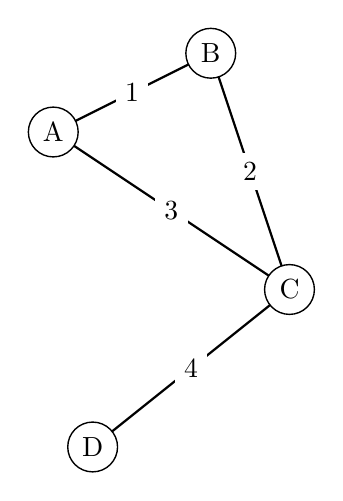
\begin{tikzpicture}[transform shape]
  \Vertex[x=0,y=0]{A}
  \Vertex[x=2,y=1]{B}
  \Vertex[x=3,y=-2]{C}
  \Vertex[x=0.5,y=-4]{D}
  \Edge[label=1](A)(B)
  \Edge[label=2](B)(C)
  \Edge[label=3](A)(C)
  \Edge[label=4](D)(C)
\end{tikzpicture}
\caption{Example Graph, I.}
\end{figure}

which we can represent via a table listing edges and vertices as follows:

\bee
\begin{array}{c|c}
edge & vertices\\
\hline
1 & A,B\\
2 & B,C\\
3 & A,C\\
4 & C,D
\end{array} 
\eee
%
The idea for the proof is to count the number of vertices in the right column in two different ways:

\begin{itemize}
\item The number of entries in the right column is two times the number od edges. In the example graph, we have $4$ edges, and $2\times 4 = 8$ entries in the right column.

\item The degree of a vertex is equal the number of times it occurs in the table. In the example graph, e.g. the vertex A has degree and occurs two times in the table. Summing over the degree of all vertices yields the number of entries in the right column.

\end{itemize}

Equating both sides therefore yields

\bee
\sum_{x \in \Vc(G)} \deg(x) = 2 |\Ec(G)|
\eee
%
A bit less formal proof, is the observation that summing over all edge degrees counts the edges twice; in the example graph, edge 1 is counted when we add the degree of vertex ``A'' and the degree of vertex ``B''. This also yields above equation.
%
Anyway, looking at the equation, we observe the following

\begin{itemize}

\item The righ-hand side is even.

\item For the left-hand side, we see that a sum with an even number of odd terms is even (e.g. $1 + 1 = 2$, $1+3+3+1 = 8$).
  
\end{itemize}

This proves the theorem stated above. \qed

In the example graph above, verices ``C'' and ``D'' had odd degree; wWe can play around a bit further and add another vertex to the graph like below.

\begin{figure}[H]
\centering
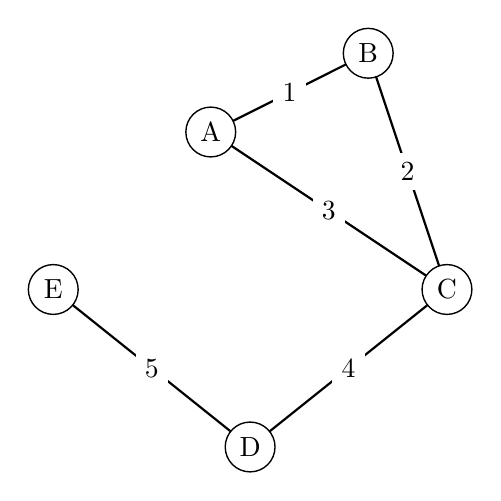
\begin{tikzpicture}[transform shape]
  \Vertex[x=0,y=0]{A}
  \Vertex[x=2,y=1]{B}
  \Vertex[x=3,y=-2]{C}
  \Vertex[x=0.5,y=-4]{D}
  \Vertex[x=-2,y=-2]{E}
  \Edge[label=1](A)(B)
  \Edge[label=2](B)(C)
  \Edge[label=3](A)(C)
  \Edge[label=4](D)(C)
  \Edge[label=5](D)(E)
\end{tikzpicture}
\caption{Example Graph, II.}
\end{figure}

Vertex ``C'' has still odd degree, but vertex ``D'' now has even degree and the new vertex``E'' has odd degree: The number of vertices with odd degree is still even.


\subsubsection{Complete Graphs}

In a complete graph with $n$ vertices, all vertices are connected with each other. To calculate the number of edges, we observe that every vertex is connected with the remaining $n-1$ vertices. If we take $n(n-1)$, we count every edge double; Therefore, the total number of edges is

\bee
|\Ec(\Gc)| = \frac{n(n-1)}{2}
\eee

Some examples of complete graphs are shown below. For $n=3$ vertices we have $\frac{3 \times 2}{2} = 3$ edges, for $n=4$ vertices we have $\frac{4 \times 3}{2} = 6$ edges, and for $n=5$ vertices we finally have $\frac{5 \times 4}{2} = 10$ edges.

\begin{figure}[H]

\begin{subfigure}{0.4\textwidth}
  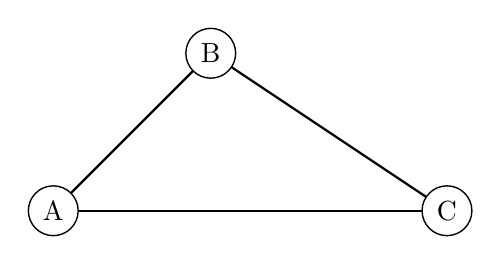
\begin{tikzpicture}[scale=1.0, transform shape]
    \Vertex[x=0,y=0]{A}
    \Vertex[x=2,y=2]{B}
    \Vertex[x=5,y=0]{C}
    \Edge(A)(B)
    \Edge(B)(C)
    \Edge(A)(C)
  \end{tikzpicture}
\caption{$n=3$ vertices.}
\end{subfigure}
\qquad % this is important, otherwise the figures won't be next each other...
\begin{subfigure}{0.4\textwidth}
  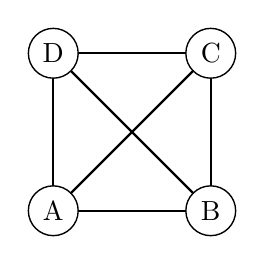
\begin{tikzpicture}[scale=1.0, transform shape]
    \Vertex[x=0,y=0]{A}
    \Vertex[x=2,y=0]{B}
    \Vertex[x=2,y=2]{C}
    \Vertex[x=0,y=2]{D}
    \Edge(A)(B)
    \Edge(A)(C)
    \Edge(A)(D)
    \Edge(B)(C)
    \Edge(B)(D)
    \Edge(C)(D)
  \end{tikzpicture}
\caption{$n=4$ vertices.}
\end{subfigure}
\end{figure}



\begin{problem}
We have a disconnected graph with $10$ vertices. Show that this graph has at most $36$ edges.
\end{problem}

Since the graph is disconnected, it contains of (at least) two components. Assume the first component has $m$ vertices, the other $10 - m$. The total number of edges is then

\bee
|\Ec(\Gc)| = \frac{m(m-1)}{2} + \frac{(10-m)(10-m-1)}{2}
\eee

We guess that this expression attains its maximum of $36$ at $m=1$ and $m=9$. In these extreme cases (one component with $9$ vertices, the other component with just $1$ vertex), the total number of edges is $36$; in all other cases it is less and this completes the proof. \qed 



\subsection{Eulerian Graph}

\begin{definition}
A closed path through a graph which uses every edge exactely once is called an Eulerian circuit. A finite graph with no isolated vertices that contains such a path is an Eulerian graph.
\end{definition}

There is a condition on whether a graph is Eulerian or not stated in the following theorem.

\begin{theorem}
A finite graph with no isolated vertices is Eulerian iff it is connected and every vertex has evn degree.
\end{theorem}

The path enters a vertex through some edge and leaves by another edge; therefore all verices must have even degree. To show that this condition is sufficient, start in a vertex ``A'' and begin a path. Keep going, not using the same edge twice until we cannot go further. Since every vertex has even degree, this can only happen when we return to ``A'' and we have used all edges from ``A''. If there are unsued edges from ``A'', we start making another path from / to these edges until all edges are used up. Finally, shorter paths can be combined into longer ones until the complete graph has been traversed. \qed

\paragraph{Example.} Some simple examples are shown in the following Figure. On the left, the simplest Eulerian circuit construction starts in vertex ``A'' and goes along ``B'', ``C'', ``D'', ``E'', returns to ``A'' from there. Slightly trickier is to start in ``B'', go via ``C'', ``D'' back to ``B''. However, not all edges from ``B'' are used, so we start another walk from ``B'' via ``A'', ``E'' and back to ``B''. The Eulerian circuit is then the combination of these two paths. On the right, we can also start in ``B'' and create two subpaths as above: ``B'', ``C'', ``D'', ``B'' and ``B'', ``E'', ``A'', ``B''. This leaves the path ``E'', ``F'', ``D'', ``G'', ``E'' out. However, we merge these three paths into one Eulerian circuit.

In any case, note that all paths have vertices with even degree.

\begin{figure}[H]

\begin{subfigure}{0.4\textwidth}
  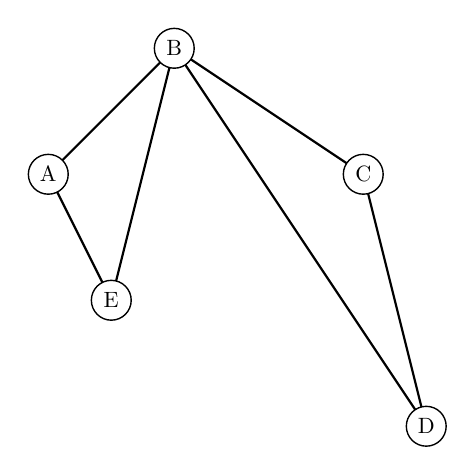
\begin{tikzpicture}[scale=0.8, transform shape]
    \Vertex[x=0,y=0]{A}
    \Vertex[x=2,y=2]{B}
    \Vertex[x=5,y=0]{C}
    \Vertex[x=6,y=-4]{D}
    \Vertex[x=1,y=-2]{E}
    \Edge(A)(B)
    \Edge(B)(C)
    \Edge(C)(D)
    \Edge(B)(D)
    \Edge(A)(E)
    \Edge(B)(E)
  \end{tikzpicture}
\caption{Euler, I.}
\end{subfigure}
\qquad % this is important, otherwise the figures won't be next each other...
\begin{subfigure}{0.4\textwidth}
  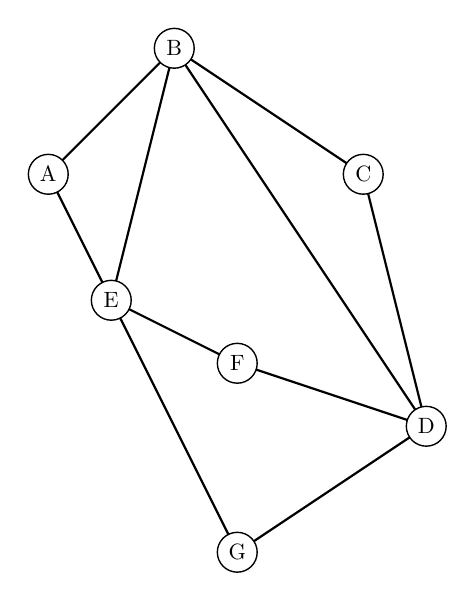
\begin{tikzpicture}[scale=0.8, transform shape]
    \Vertex[x=0,y=0]{A}
    \Vertex[x=2,y=2]{B}
    \Vertex[x=5,y=0]{C}
    \Vertex[x=6,y=-4]{D}
    \Vertex[x=1,y=-2]{E}
    \Vertex[x=3,y=-3]{F}
    \Vertex[x=3,y=-6]{G}
    \Edge(A)(B)
    \Edge(B)(C)
    \Edge(C)(D)
    \Edge(B)(D)
    \Edge(A)(E)
    \Edge(B)(E)
    \Edge(E)(F)
    \Edge(E)(G)
    \Edge(D)(F)
    \Edge(D)(G)
  \end{tikzpicture}
\caption{Euler, II.}
\end{subfigure}
\end{figure}

\DiaryEntry{Graphs, Trees}{2017-04-11}{Graphs}

\subsection{General}


\begin{definition}
A graph is called a tree if it is connected and contains no cycle as a subgraph.
\end{definition}

The two defining properties are somewhat opposite: The connectedness part ensures that the graph does not have ``too few'' edges, whereas the ``no cycles'' part ensures that the graph has not ``too many'' edges.

If a graph is connected, then it will stay connected when we add another edge. If we remove an edge, the graph may become disconnected. If a graph has no cycles, it will still have no cycles if we remove another edge. If a graph has no cycles, it may become cycles if we add another edge.

In that sense a tree is a ``minimally connected'' subgraph or a ``maximally cycle-free'' graph:

\begin{theorem}
(i) A graph is a tree if and only if it is connected, but deleting any of its edges results in a disconnected graph. (ii) A graph is a tree if and only if it contains no cycles, but adding any new edge creates a cycle.
\end{theorem}

For (i) we want to show that a tree cannot stay connected if we remove an edge. Assume that the edge $u-v$ is deleted from the graph $G$ and the resulting graph $G'$ stays connected. This implies that there is a path from $u$ to $v$. However, if we put the edge $u-v$ back, the path and the edge $u-v$ will form a cycle and that contradicts the definition of a tree.

(ii) follows with a similar argument.

Assume we have a connected graph with $n$ nodes and an edge $e$. If we obtain a disconnected graph by deleting $e$, then $e$ is called a cut-edge. With this definition, every edge of a tree is a cut-edge.

A spanning tree of a graph is a subgraph that has the same nodes but is a tree. We can obtain a spanning tree from a graph by deleting edges from the graph until a graph is obtained that is still connected, but deleting any further edge makes it disconnected; by definition, this is a tree. The edge deletion process can be carried out in many different ways; therefore, the spanning tree of a graph is not unique.

\begin{theorem}
  Every tree on $n$ vertices has $n-1$ edges.
\end{theorem}

We can prove this via induction: We start the tree with two vertices and an edge connecting the two. Adding one edge after the other, keeps the different between the number of edges and the number of vertices the same.

The converse, however is not true; i.e. a graph with $n$ vertices and $n-1$ edges is not necessarily a tree. Consider the example below.

\begin{figure}[H]
\centering
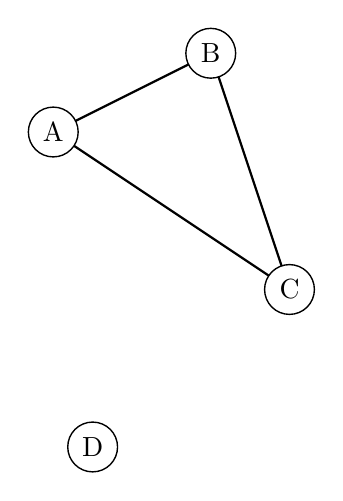
\begin{tikzpicture}[transform shape]
  \Vertex[x=0,y=0]{A}
  \Vertex[x=2,y=1]{B}
  \Vertex[x=3,y=-2]{C}
  \Vertex[x=0.5,y=-4]{D}
  \Edge(A)(B)
  \Edge(B)(C)
  \Edge(A)(C)
\end{tikzpicture}
\caption{Trees.}
\end{figure}




%\DiaryEntry{Cyclic Codes, I}{2017-04-18}{Coding}

\subsection{Repetition - Rings}

\begin{definition}
  A ring $(R,+,\cdot)$ is a set $R$ with two binary opeations, $+$ (addition) and $\cdot$ (multiplication), defined on $R$ such that

  \begin{itemize}
    \item $(R,+)$ forms an abelian group with additive identity typically denoted as $0$.
    \item The multiplication operation $\cdot$ is associative: $(a \cdot b) \cdot c = a \cdot (b \cdot c)$ for $a,b,c \in R$.
    \item Left and right distributive laws hold: $a(b+c) = ab + ac, (a+b)c = ac + bc$
  \end{itemize}
%
  A ring is commutative if $a \cdot b = b \cdot a$, for all $a,b \in R$. A ring is said to be a ring with identity if $\cdot$ has an identitiy element which is typically denoted as $1$.

\end{definition}

As a simple example, consider $(\mZ_6, +, \cdot)$ with addition and multiplication tables as follows (addition and multiplication are taken modulo-6):

\begin{figure}[H]
  \includegraphics[scale=0.75]{images/cyclic_codes_01.png}
\end{figure}

Note that the set does not form a group under multiplication (it does under addition, though). However, this does not contradict the ring definition; i.e. it is a ring.


\subsection{Repetition - Rings of Polynomials}

If $R$ is a ring, then the set of all polynomials with coefficients in $R$ form a ring under the usual operations for polynomial addition and multiplication. This ring is denoted as $R[x]$, where $x$ is the polynomial variable:

\bee
f(x) = \sum_{i=0}^n a_i x^i, a_i \in R
\eee

Addition (adding coefficients with the same degree according to the ring operation) of polynomials yields another polynomial in the ring, the same holds for multiplication. The inverrse of a polynomial will in general not be another polynomial (e.g. $(1 + 4x)^{-1}$), but note that a ring need not have multiplicative inverses (it's not a field after all).

\paragraph{Example.} Taking $R$ to be $(\mZ_6, +, \cdot)$, we obtain a polynomial ring as $R[x]$ with some example elements $f_1(x) = 3 + x, f_2(x) = 5 + 3x^2$. For example, we have $f_1 + f_2 = 2 + x + 3x^2$ and $f_1 f_2 = 3 + 5x + 3x^2 + 3x^3$.

\subsection{Repetition - Quotient Rings}

In Group Theory, a set of cosets was created by ``translating'' a subgroup; i.e. if $H$ is a subgroup of a group $G$, then we formed cosets by $g + H, g \in G$.

In a similar spirit, we can collect polynomials over a ring into equivalence classes by their remainder after division by a fixed polynomial.

As an example, consider the ring of polynomials $GF(2)[x]$ and a fixed polynomial $x^3+1$. Now collect all polynomials with remainder $0$ after division modulo $x^3+1$:

\bee
S_0 = \{0, x^3+1, x^4+x, x^5+x^2, \ldots\} = \langle x^3 + 1 \rangle
\eee

where $S_0 = \langle x^3 + 1 \rangle$ is the set of polynomials generated by $x^3+1$. Note that $S_0$ is actually a subring: Denote $p_1(x), p_2(x)$ two polynomials with remainder $0$ after division by $x^3+1$. The sum $p_1(x) + p_2(x)$ will also have a remainder $0$ after division by $x^3+1$

\bee
\frac{p_1(x) + p_2(x)}{x^3+1} = \frac{p_1(x)}{x^3+1} + \frac{p_2(x)}{x^3+1} \equiv 0 \bmod (x^3+1)
\eee

and in a similar spirit, the multiplication as well

\bee
\frac{p_1(x)p_2(x)}{x^3+1} = \frac{p_1(x)}{x^3+1} \frac{p_2(x)}{x^3+1} \equiv 0 \bmod (x^3+1)
\eee

The set $S_1$ contains all polynomials with remainder $1$ after division modulo $x^3+1$:

\bee
S_1 = \{1, x^3, x^4+x+1, x^5+x^2+1, \ldots\} = 1 + \langle x^3 + 1 \rangle
\eee

Noe that his is not a (sub)ring as it does not contain the identity element. The other equivalence classes are obtained in the same manner.

\begin{figure}[H]
  \includegraphics[scale=0.65]{images/cyclic_codes_02.png}
\end{figure}

By dividing through $x^3+1$, only 7 different remainders are possible: $0, 1, x, 1+x, 1+x^2, x+x^2, 1+x+x^2$. Therefore, all polynomials of $GF(2)[x]$ fall into of these equivalence classes.

In a similar spirit to defining an induced operation of cosets, we can define induced operations $+$ and $\cdot$ for the equivalence classes of polynomials modulo $x^3+1$ by operation on representative elements. We obtain the following tables:

\begin{figure}[H]
  \includegraphics[scale=0.65]{images/cyclic_codes_03.png}
\end{figure}

As an example, note that $S_3 + S_5 = S_6$. Adding one of the corresponding elements from the cosets yields $(x+1) + (x^2+1) \equiv x^2+x$, which corresponds to $S_6$. For multiplication, let us take $S_3 S_7 = S_0$, corresponding to the following polynomial identitiy: $(x+1)(x^2+x+1) \equiv x^3+1$ which corresponds to $S_0$.

If we define $R=\{S_0, S_1,\ldots, S_7\}$, then $(R,+)$ is an Abelian group with $S_0$ as identity and for multiplication $S_1$ acts as identity. Not every element has a multiplicative inverse, so $R - S_0$ is not a group. However, the whole thing $(R,+,\cdot)$ is a ring denoted as $GF[x]/\langle x^3+1 \rangle$.

In the general case, denote a ring $GF(2)[x]/\langle x^n-1 \rangle$ as $R_n$ and a ring $\mF_q[x]/\langle x^n-1\rangle$ as $R_{n,q}$.

\paragraph{General Case.} For a field $\mF$ (with $q$ elements), the associated ring of polynomials $\mF[x]$ can be partitioned by a polynomial $f(x)$ of degree $m$ into $q^m$ different equivalence classes with one equivalence class for each remainder modulo $f(x)$. This ring is denoted as $\mF[x]/\langle f(x)\rangle$ or $\mF[x]/f(x)$.

As a side note (which will be proven later on), we note that the ring $\mF[x]/f(x)$ is a field iff the polynomial $f(x)$ cannot be factored over $\mF[x]$. In the example above, we have $x^3+1 = (x+1)(x^2+x+1)$ so $\mF[x]/(x^3+1)$ is not a field.



\subsection{Ideals in Rings}

\begin{definition}
  Let $R$ be a ring. A nonempty subset $I \subseteq R$ is an ideal if

  \begin{itemize}
    \item $I$ forms a group under addition in $R$.
    \item For any $a \in I$ and $r \in R$, $ar \in I$.
  \end{itemize}
\end{definition}

The first point ensures that the ideal has a structure; i.e. adding two ideal elements yields another ideal element. The second point is interesting in that the product of an ideal and a ``non-ideal'' element is still an ideal.

As a simple example, take $R$ as the set of integers. An ideal is the set of even numbers; the sum of any two even numbers is even and the product of any number with an even one gives an even number.

\begin{definition}
  An ideal $I$ in a ring $R$ is said to be principal if there exists some $g \in I$ such that every element $a \in I$ can be expressed as a product $a = mg$ for some $m \in R$. For a principal ideal, such an element $g$ is called the generator element. The ideal generated by $g$ is denoted as $\langle g \rangle$:

  \bee
    \langle g \rangle = \{hg : h \in R\}
  \eee
  
\end{definition}

The ideal in the example above is principal with a generator element $g = 2$. Every element of the ideal can be created by $2m$ with $m \in R$.

\begin{theorem}
  Let $I$ be an ideal in $\mF_q[x] / \langle x^n-1 \rangle$. Then
  \begin{itemize}
    \item There is a unique monic polynomial $g(x) \in I$ of minimal degree.
    \item $I$ is principal with generator $g(x)$.
    \item $g(x)$ divides $(x^n-1)$ in $\mF_q[x]$.
  \end{itemize}

\end{theorem}

\paragraph{Example.}Consider the polynomial $x^7+1$ over $GF(2)[x]$ which can be factored as

\bee
x^7 + 1 = (x+1)(x^3 + x + 1)(x^3 + x^2 + 1)
\eee

This factorization can be obtained in GAP via the following commands

\begin{verbatim}
a:=GF(2);
x:=X(GF(2));
Factors(p);
   [ x_1+Z(2)^0, x_1^3+x_1+Z(2)^0, x_1^3+x_1^2+Z(2)^0 ]
\end{verbatim}

Any combination of these 3 factors can be used as generator for a principal ideal.

\paragraph{Example.} A simpler example uses the polynomial $p(x) = x^3+1 = (x+1)(x^2+x+1)$. Choosing as generator $g_1(x) = x+1$, we can calculate the ideal by multiplying $g_1(x)$ with the elements of $GF(2)[x]/x^3+1 = \{0,1,x,1+x, x^2, x^2+1, x^2+x, x^2+x+1\}$ (and taking modulo-$x^3+1$). We can do this in GAP with the following script

\begin{verbatim}
a:=GF(2);
x:=X(GF(2));

# let's take the first factor, x+1 as generator for an ideal

GElements := [0,1,x,1+x,x^2,x^2+1,x^2+x, x^2+x+1];
p1 := x+1;

for e in GElements do
   Print(e,"...", e*p1 mod p, "\n");
od;
\end{verbatim}

There are some duplicates; after removal of them we obtain the ideal $I_1 = \{0, x+1, x^2+1, x^2+x\}$. The sum of two ideal elements is again an ideal element (``proof'' by going over all combinations) and the product of an ideal element and any element of $GF(2)[x]/x^3+1$ is again in the ideal $I_1$ (``proof'' by going over all combinations).

\subsection{Cyclic Codes}

A cyclic shift of a binary code word looks like this: We have a vector $\cbf = (c_0, c_1, \ldots,c_{n-2}, c_{n-1})$ and shift it cyclically to the right to obtain $\cbf' = (c_{n-1}, c_0, c_1, \ldots, c_{n-2})$.

\begin{definition}
  An $(n,k)$ block code is cyclic, it it is linear and if for every codeword, its right cyclic shift is also a codeword.
\end{definition}


This cyclic shifting can be expressed in terms of polynomial manipulations; If we have the codeword

\bee
\cbf = (c_0, c_1, \ldots,c_{n-2}, c_{n-1})
\eee
%
we can associate the polynomial

\bee
c(x) = \cbf = c_0 + c_1 x + c_2 x^2 + \cdots c_{n-1} x^{n-1}
\eee
%
A non-cyclic right-shift is then represented as $xc(x)$ and a cyclic right-shift is represented by $xc(x) \mod (c^n-1)$.


\DiaryEntry{GCD}{2017-04-26}{Algebra}

\subsection{Basics}

\begin{definition}
The greatest common divisor (GCD) of two numbers is defined the largest integer that divides both of the numbers. If the greatest common divisor is 1, this means that there are no prime factors in common. We say the numbers are coprime in this case.
\end{definition}

In GAP, we can calculate the gcd of two numbers as follows

\begin{verbatim}
gap> GcdInt(3,4);
1
gap> GcdInt(3,6);
3
gap> GcdInt(8,12);
4
\end{verbatim}

\begin{theorem}
The Greatest Common Divisor Theorem. Given two positive integers $x$ and $y$, the greatest common divisor of $x$ and $y$ is the smallest positive integer which can be expressed in the form

\bee
ux + vy
\eee
%
with $u$ and $v$ being integers.
\end{theorem}

We can do that with GAP as follows

\begin{verbatim}
gap> Gcdex(8,12);
rec( coeff1 := -1, coeff2 := 1, coeff3 := 3, coeff4 := -2, gcd := 4 )
\end{verbatim}

We have $-1 \times 8 + 1 \times 12 = 4$ as in the theorem above; however, we get some more information in that $(-1 + 3) \times 8 + (1 - 2) \times 12 = 4$.

\paragraph{Proof.} Denote the set of positive numbers which can be expressed in the form $ux + vy$ as $\Ac$ and denote the smallest such number as $n$. Since $\gcd(x,y)$ is a factor of both $x$ and $y$, it must also be a factor of $n$. Next, consider $k \equiv x (\mod n)$ which must fulfill $0 \leq k < n$ and therefore $k = x + nr$ for some number $r$. 

We can now insert the expression for $n$ and obtain $k = x + (ux + vy)r = (1+ru)x + (rv)y$ for some numbers $u, v$. This shows that $k \in \Ac$. 

We assumed $n$ to be the smallest number in $\Ac$, $k$ cannot be equivalent $\mod n$ to any number less than $n$, other than $0$. Therefore, $x \equiv 0 \mod n$ and $n$ is a divisor of $x$. Similar reasoning yields that also $n$ is a divisor of $y$. Thus, $n$ is a common divisor of $x,y$ and since $\gcd(x,y)$ is also a divisor of $n$, $n = \gcd(x,y)$. \qed


\begin{theorem}[Chinese Remainder Theorem]
If $u,v \in \mZ^{+}$ are coprime, then given any $x,y \in \mZ$, there is a unique $k \in \mZ$ such that

\bee
0 \leq k < uv
\eee
%
and
\bee
k \equiv x \bmod u \qquad k \equiv y \bmod v
\eee
\end{theorem}

\paragraph{Proof.} 
We show first that there cannot be \emph{more} than one such number $k$: Suppose there are two different, $k$ and $q$, which satisfy above conditions; i.e. $k \equiv x \bmod u$ and $q \equiv x \bmod u$. We can subtract both equations from each other to obtain $k - q \equiv 0 \bmod u$ and in a similar spirit $k - q \equiv 0 \bmod v$. Therefore, $k-q$ must be a multiple of both $u$ and $v$. Since $u$ and $v$ are coprime, the least common multiple must be $uv$ and therefore $k-q$ is a multiple of $uv$. However, both $k$ and $q$ are less than $uv$. The only way this is possible is that $k-q=0$ but this contradicts the assumption that there are different $k$ and $q$. So we have shown that there is a unique value $k$.

The second part of the proof shows that there must \emph{exist} such a $k$: For any number $k$, the expression $k \bmod u$ takes on $u$ different values, from $0$ to $u-1$. Analogously, $k \bmod v$ takes on $v$ different values, from $0$ to $v-1$. For any $k$, there are only $uv$ possible ordered pairs of the form $(k \bmod u, k \bmod v)$.

So, no two values of $k$ between $0$ and $uv-1$ can give the same ordered pair. But there are exactly $uv$ such values of $k$. By the pigeonhole principle, since each of the $uv$ possible values of $k$ produces one of the $uv$ possible ordered pairs, and no two $k$’s can produce the same ordered pair, each ordered pair must be produced by some (unique) value of $k$. \qed


\subsection{Connections to Groups}

In previous posts, we considered finite groups (consisting of the elements $1 \ldots n$) with group operation to be multiplication modulo $n$. One interesting question is whether a group element has an inverse or not. The following theorem answers this question.

\begin{theorem}
For $n$ being a positive integer, then a group element $x$ ($0 \leq x < n$) has a multiplicative inverse modulo-n, iff $x$ is coprime to $n$.
\end{theorem}

\paragraph{Proof.} If $x$ and $n$ are not coprime, they have a common factor which we call $p$. We then have $x = ap, y = bp$ and $xy = abp^2$; i.e. $xy$ is a multiple of $p$. In order for $x$ to have a multiplicative inverse, there must be a $y$ such that

\bee
x y \equiv 1 \bmod n
\eee
%
This means $xy = 1 + wn$ for some integer $w$. But since $xy$ is already a multiple of $p$ (see above), $xy$ can not also be a multiple of $1 + wn$.


\paragraph{Group Definition.} Based on this theorem, we then define the group $\mZ_n^\star$ with group operation multiplication modulo-$n$ and elements $x < n$ being coprime with $n$. The number of group elements of $\mZ_n^\star$ depends on how many nummber are coprime to $n$ and this value is given by the \emph{Euler totient function} of $n$, denoted by $\Phi(n)$.


\subsection{Euler Totient Function}

If a prime factorization of $n$ is given by

\be
\label{gcd_01:pf}
n = p_1^{r_1} p_2^{r_2} \cdots p_k^{r_k}
\ee

where the $p_i$ are distinct primes and the $r_i$ are positive integers, then

\bee
\Phi(n) = (p_1 - 1)p_1^{r_1-1} (p_2 - 1)p_2^{r_2-1} \cdots (p_k - 1)p_k^{r_k-1}
\eee


\paragraph{Proof.} To begin, if $p$ is prime, then it has $p-1$ coprime values smaller than $p$: $\Phi(p) = p-1$. If we consider $p^r$ as a next step, then the only numbers not coprime to $p^r$ are multiples of $p: p, 2p, 3p, \ldots p^r$. That's $1/p$ of all numbers; the remaining $(1-1/p)p^r$ will be coprime. This can be rewritten as $(p-1)p^{r-1}$ and we have $\Phi(p^r) = (p-1)p^{r-1}$.

Without proof (for now), we also note that if $m$ and $n$ are coprime, then $\Phi(m,n) = \Phi(m) \Phi(n)$.

Looking at \eqref{gcd_01:pf}, we see that all factors of $n$ are coprime (they are powers of prime numbers). So we have $\Phi(n) = \Phi(p_1^{r_1}) \cdots \Phi(p_k^{r_k}) = (p_1 - 1)p_1^{r_1-1} \cdots (p_k - 1)p_k^{r_k-1}$. \qed

We can write the expression for $\Phi(n)$ a bit different by using the fact from above that $\Phi(p^r) = (1-1/p)p^r$ and therefore

\bee
\Phi(n) = (1-1/p_1)p_1^{r_1} \cdots (1-1/p_k)p_k^{r_k} = n (1 - 1/p_1) \cdots (1 - 1/p_k) = n \prod_{p | n} \left(1 - \frac{1}{p} \right)
\eee
%
This is (maybe) the more classical representation of the totient function.

\paragraph{Function Plot}

The following Figure shows a plot of $\Phi(n)$. The upper bound of $\Phi(n) = n-1$ for $n$ being prime can be seen.

\DiaryEntry{GCD - Algorithms}{2017-05-01}{Algebra}


\subsection{Euclidean Algorithm}

\subsubsection{Basics}

\begin{theorem}
Assume that $a \geq b$, then we have the fact that $\gcd(a,b) = \gcd(a - b,b)$.
\end{theorem}

\paragraph{Proof.} Let $g = \gcd(a,b)$, then $a = a' g$ and $b = b' g$, with $a', b'$ being relatively prime (i.e. their gcd is $1$). Now, $a - b = g(a' - b')$ and therefore shares $g$ as common factor with $a = a'g$. In other words, $a' - b'$ and $a'$ are relatively prime. If this were not the case, we could write $a - b = g \tilde{g}(a'' - b'')$ and $a = a'' \tilde{g}g$ but this contradicts the fact that $g = \gcd(a,b)$. \qed

By repeatedly subtracting $b$ from $a$ (until a value smaller than $b$ is left), we arrive at the following identity

\be\label{gcd_02_1}
\gcd(a,b) = \gcd(a \bmod b, b)
\ee

\subsubsection{Algorithm.}

The principle behind the algorithm is to use \eqref{gcd_02_1} to subsequently reduce the values of $a$ and $b$, until one of them becomes zero. That's the end of the algorithm (we have $\gcd(x,0) = x$).

The algorithm starts with $a$ and $b$ and finds the greatest common divisor $\gcd(a,b)$. The algorithm proceeds in a series of steps and the integer $k$ counts the steps of the algorithm. The algorithms starts with $k=0$.

Each step takes two integers $r_{k-1}, r_{k-2}$ and calculates $q_k, r_k$ as follows

\bee
r_{k-2} = q_k r_{k-1} + r_k, \qquad r_k < r_{k-1}
\eee
%
In other words, multiples of the smaller number $r_{k-1}$ are subtracted from the larger number $r_{k-2}$ until the remainder $r_k$ is smaller than $r_{k-1}$.
%
Initially ($k=0$), $r_{-2} = a, r_{-1} = b$. For subsequent steps, we have

\begin{align*}
  a &= q_0 b + r_0 \\
  b &= q_1 r_0 + r_1 \\
  r_0 &= q_2 r_1 + r_2 \\
  r_1 &= q_3 r_2 + r_3 \\
  &\cdots  
\end{align*}

The algorithm ends, when a remainder $r_N$ becomes zero. Then $\gcd(a,b) = r_{N-1}$.

\subsubsection{Example}

As a first example, let us calculate $\gcd(1071, 462)$:

\begin{align*}
  1071 &= 2 \times 462 + 147 \\
  462 &= 3 \times 147 + 21 \\
  147 &= 7 \times 21 + 0
\end{align*}

With this the algorithm stops (the remainder is $0$) and the gcd becomes the previous remainder; i.e. $\gcd(1071, 462) = 21$.

As second example, consider $\gcd(1071, 463)$:

\begin{align*}
  1071 &= 2 \times 463 + 145 \\
  463 &= 3 \times 145 + 28 \\
  145 &= 5 \times 28 + 5 \\
  28 &= 5 \times 5 + 3 \\
  5 &= 1 \times 3 + 2 \\
  3 &= 1 \times 2 + 1 \\
  2 &= 1 \times 1 + 0
\end{align*}

Therefore, we have $\gcd(1071, 463) = 1$.


%\DiaryEntry{The Groups $\mZ_n$ vs $\mZ_n^\star$}{2017-05-05}{Algebra}

\subsection{The Group $\mZ_n$}

This group contains the integers $0 \ldots n-1$ and has group operation addition modulo-$n$. A simple example is $\mZ_5$ with ``multiplication'' (group operation table is probably better) table as follows

\bee
\begin{array}{c|ccccc}
\star & 0 & 1 & 2 & 3 & 4 \\ \hline
0     & 0 & 1 & 2 & 3 & 4 \\
1     & 1 & 2 & 3 & 4 & 0 \\
2     & 2 & 3 & 4 & 0 & 1 \\
3     & 3 & 4 & 0 & 1 & 2 \\
4     & 4 & 0 & 1 & 2 & 3
\end{array}
\eee

\paragraph{Generators.} An element $x$ of a group $G$ is called \emph{generator}, if every element of $G$ can be expressed as power of $x$.

Next question is which elements of the group are generators. We have the following theorem:

\begin{theorem}
The generators of $\mZ_n$ are those integers between $0$ and $n-1$ which are coprime to $n$. There are $\Phi(n)$ such numbers; therefore, $\mZ_n$ has $\Phi(n)$ generators.
\end{theorem}

\paragraph{Proof.} Suppose $g$ is a generator of $\mZ_n$. Then $1$ can be expressed as power of $g$; i.e.

\bee
g^v \equiv 1 \bmod n
\eee

for some integer $v$. In case of $\mZ_n$, the group operation is not multiplication but addition (modulo-$n$), so we should write

\bee
v g \equiv 1 \bmod n
\eee

instead. This says, that $v$ is the inverse of $g$ and from the post in Section \ref{2017-04-26:entry}, we know that this inverse $v$ exists only if $g, n$ are coprime. So in the following, assume that $g,n$ are coprime; i.e. there is a $v$ fulfilling above condition and $1$ can be expressed as ``power'' of $g$. 

But $1$ is a generator of $\mZ_n$; in other words, every element of $\mZ_n$ can be expressed as $w 1$ (with some integer $w$). Inserting the expression for $1$ from above, we have that every element can be expressed as $w 1 = w (v g) = (wv)g$; i.e. every element can be expressed as ``power'' of $g$. \qed

In the example of $\mZ_5$, things are simple as every element is coprime to $5$ ($5$ is a prime). Indeed, we have

\bee
1 \cdot 1 \equiv 1 \bmod 5, 2 \cdot 1 \equiv 2 \bmod 5, 3 \cdot 1 \equiv 3 \bmod 5 , 4 \cdot 1 \equiv 4 \bmod 5, 5 \cdot 1 \equiv 0 \bmod 5
\eee

and

\bee
1 \cdot 2 \equiv 2 \bmod 5, 2 \cdot 2 \equiv 4 \bmod 5 , 3 \cdot 2 \equiv 1 \bmod n, 4 \cdot 2 \equiv 3 \bmod 5, 5 \cdot 2 \equiv 0 \bmod 5
\eee

and

\bee
1 \cdot3 \equiv 3 \bmod 5, 2 \cdot 3 \equiv 1 \bmod 5, 3 \cdot 3 \equiv 4 \bmod 5, 4 \cdot 3 \equiv 2 \bmod 5, 5 \cdot 3 \equiv 0 \bmod 5
\eee

and finally

\bee
1 \cdot 4 \equiv 4 \bmod 5, 2 \cdot 4 \equiv 3 \bmod 5, 3 \cdot 4 \equiv 2 \bmod 5, 4 \cdot 4 \equiv 1 \bmod 5, 5 \cdot 4 \equiv 0 \bmod 5
\eee

so all elements of $\mZ_5$ are also generators.

As counterexample, consider $\mZ_4$ with the following group operation table

\bee
\begin{array}{c|ccccc}
\star & 0 & 1 & 2 & 3  \\ \hline
0     & 0 & 1 & 2 & 3  \\
1     & 1 & 2 & 3 & 0  \\
2     & 2 & 3 & 0 & 1  \\
3     & 3 & 0 & 1 & 2
\end{array}
\eee

Checking all elements for generators, we obtain the following result

\bee
1 \cdot 1 \equiv 1 \bmod 4, 2 \cdot 1 \equiv 2 \bmod 4, 3 \cdot 1 \equiv 3 \bmod 4, 4 \cdot 1 \equiv 0 \bmod 4
\eee

so $1$ is a generator. For $2$, we have 

\bee
1 \cdot 2 \equiv 2 \bmod 4, 2 \cdot 2 \equiv 0 \bmod 4, 3 \cdot 2 \equiv 2 \bmod 4, 4 \cdot 2 \equiv 0 \bmod 4
\eee

which does not produce all elements; so no generator. With $2$ not being coprime with $4$, everything is accordance with the above theorem. For $3$, we have

\bee
1 \cdot 3 \equiv 3 \bmod 4, 2 \cdot 3 \equiv 2 \bmod 4, 3 \cdot 3 \equiv 1 \bmod 4, 4 \cdot 3 \equiv 0 \bmod 4
\eee

so $3$ is a generator (it is coprime with $4$).


\subsection{The Group $\mZ_n^\star$}

Here, we know from entry \ref{2017-04-26:entry}, that $\mZ_n^\star$ contains all integers $x < n$ which are coprime with $n$ and that there are $\Phi(n)$ such elements.

Another notation for this group is $(\mZ / n \mZ)^\times$ (see \href{https://en.wikipedia.org/wiki/Multiplicative_group_of_integers_modulo_n}{Wikipedia}).

The Wikipedia article is actually quite comprehensive; e.g. it lists the generators for a group $\mZ_n^\star$.

As an example, consider the group $\mZ_4^\star$; $\Phi(4) = 2$, so the group has the $2$ elements $\mZ_4^\star = \{1,3\}$ (the numbers coprime with $4$). The group operation table has the following form

\bee
\begin{array}{c|cc}
\star & 1 & 3  \\ \hline
1     & 1 & 3  \\
3     & 3 & 1
\end{array}
\eee

Generator is (according to Wikipedia), the element $3$ (this is actually obvious; it cannot be the identity element $1$ and there is no other element). We have

\bee
1 \cdot 3 \equiv 3 \bmod 4, 3 \cdot 3 \equiv 1 \bmod 4
\eee

therefore $3$ is a (the) generator.

A little bit more advanced is $\mZ_8^\star$ which has $\Phi(8) = 4$ elements: $\mZ_8^\star = \{1,3,5,7\}$ with group operation table

\bee
\begin{array}{c|ccccc}
\star & 1 & 3 & 5 & 7  \\ \hline
1     & 1 & 3 & 5 & 7  \\
3     & 3 & 1 & 7 & 5  \\
5     & 5 & 7 & 1 & 3  \\
7     & 7 & 5 & 3 & 1  \\
\end{array}
\eee

According to Wikipedia, the two elements $3,7$ are generators; i.e. every element of $\mZ_8^\star$ can be expressed as a combination of these two. We have

\bee
3 \cdot 3 \equiv 1 \bmod 8, 3 \cdot 7 \equiv 5 \bmod 8
\eee

and all other combinations do not contribute additional / new elements; e.g. $7 \cdot 7 \equiv 1 \bmod 8$.


\DiaryEntry{Euler's Theorem}{2017-05-08}{Algebra}

\subsection{Repetition}

\paragraph{Group Order.} Assume we have a group $G$ with an element $x$. The order $n$ of $x$ is the smallest integer so that $x^n = e$ (where $e$ denotes the group identitiy element). If $x$ is infinite, then the order is (also) infinite. Let $[x]$ denote the cyclic subgroup

\bee
[x] = \{e, x, x^2, \ldots, x^{n-1}\}
\eee

The order of this subgroup is $n$ (as $x^n = e$).

\paragraph{Lagrange Theorem.} Let $G$ be a finite group, and $H$ a subgroup of $G$. Then the order of $H$ divides the order of $G$. That is, $|G| = k |H|$ for some positive integer $k$.


Some additional statements based on the Lagrange Theorem:

\begin{itemize}

  \item Let $G$ be a finite group with element $x$. The order of the subgroup $[x]$ divides $|G|$ and since the order of $x$ equals the order of the subgroup $[x]$, the order of $x$ divides $|G|$.

  \item $x^n = e$ if $x \in G$ and $G$ being a finite order group with order $n$. Let $m$ denote the order of $x$ (and $[x]$), we have $n = mk$ by Lagrange's Theorem for some integer $k$. Then $x^n = x^{mk} = (x^m)^k = e^k = e$.

\end{itemize}


\subsection{Euler's Theorem}

\begin{theorem}

Let $n$ be a positive integer, and $x$ a number coprime to $n$. Then

\bee
x^{\Phi(n)} \equiv 1 \bmod n
\eee

with $\Phi$ being Euler's totient function.
  
\end{theorem}

\paragraph{Proof.} We consider the group $\mZ_n^\star$: The group has $\Phi(n)$ elements and if $x$ is coprime to $n$, then $x \in \mZ_n^\star$. This is exactely the situation in the second bullet point above; noting that $e = 1$ in $\mZ_n^\star$, we have proven the theorem. \qed

\begin{theorem}[Fermat's little theorem]

  When $n = p$ is prime, we have $\Phi(n) = p-1$ and therefore,
  \bee
  x^{p-1} \equiv 1 \bmod p
  \eee

\end{theorem}




%\DiaryEntry{Subgroups}{2017-06-07}{Algebra}


\begin{definition}[Subgroup]
  If G is a group, then a subset H of G is a subgroup of G if H is non-empty and H is closed under products and inverses: If $x,y \in H$, then $x^{-1} \in H$ and $xy \in H$. This is written as $H \leq G$.
\end{definition}

Proofing that a subset is actually a subgroup may be rather tedious, as all inverses and products need to be checked. Somewhat simpler is the following criteria, whether a subset $H$ is actually a subgroup of a group $G$:

\begin{enumerate}
    \item $H \neq 0$.
    \item for all $x,y \in H, xy^{-1} \in H$.
\end{enumerate}

If $H$ is a subgroup, it is not empty, so (1) holds (a subgroup contains at least the identity element). (2) holds as well, because $H$ contains the identity, the inverse of each of its elements and because $H$ is closed under multiplication.

The converse; i.e. that if a subset $H$ satisifes (1) and (2), it is a subgroup can be shown as follows: Let $x$ be any element of $H$ (this follows from property (1)). From (2) we deduce that $1 = xx^{-1} \in h$, so $H$ contains the identity of $G$. Since $H$ contains $1$ and $x$, we have by (2) $1 x^{-1} = x^{-1} \in H$ so $H$ is closed under inverses. Finally, if $x$ and $y$ are any two elements of $H$, then $H$ contains $y^{-1}$ and we have $x(y^{-1})^{-1} = xy \in H$ so $H$ is also closed under multiplication. All in all, we have shown that $H$ is a subgroup of $G$. \qed


\paragraph{Examples.}

\begin{itemize}
\item $\mZ \leq \mQ \leq \mR$ with the operation of addition.

\item The set of even integers $\{\ldots, -4, -2, 0, 2, 4, \ldots\}$ is a subset of all integers under addition: The sum of two even integers is even and every (even) integer has an inverse.

\item The set of complex numbers of the form $\{a + ai, a \in \mR\}$ is a subgroup of $\mC$: The sum of two such elements also has the same form ($a+ai + b + bi = (a+b) + (a+b)i$) and for every subgroup element there exists an inverse ($-a-ai$).

\item The set of all positive integers $\mZ^+ = \{1,2,3,\ldots\}$ is \emph{not} a subgroup of $\mZ$. It is closed under addition (the sum of two positive integers is again a positive integer), but it does not contain a neutral element ($0 \notin \mZ$) neither inverses ($-x \notin \mZ$).

\end{itemize}


\subsection{Centralizers and Normalizers}

\begin{definition}[Centralizer]
The centralizer of a set $A$ being a subset of a group $G$ is defined as

\bee
C_G(A) = \{g \in G | gag^{-1} = a, \quad \forall a \in A\} = \{g \in G | ga = ag, \quad \forall a \in A\}
\eee

\end{definition}

In other words, $C_G(A)$ is the set of elements of $G$ wich commute with every element of $A$.

We show that the centralizer is a subgroupf of $G$: First, $1 \in C_G(A)$, because the identity element $1$ is defined as $1a = a1$ for all $a \in G$ (and in particular, for all $a \in A$). Next, let $x \in C_G(A)$. Then, $xax^{-1} = a$, and left-multiplying with $x^{-1}$, right-multiplying with $x$ yields $x^{-1}ax = a$, so $x^{-1} \in C_G(A)$ and therefore the centralizer is closed under inverses. Finally, let $y \in C_G(A)$ and observe that

\bee
(xy) a (xy)^{-1} = (xy) a (y^{-1} x^{-1}) = x (y a y^{-1}) x^{-1} = x a x^{-1} = a
\eee

which shows that $xy \in C_G(A)$. Therefore $C_G(A)$ is closed under products and we have $C_G(A) \leq G$.


The \emph{center} $Z(G)$ of a group $G$ is defined as $Z(G) = \{g \in G | gx = xg, \quad x \in G \}$; i.e. it is the set of elements commuting with all group elements. In other words, we have $Z(G) = C_G(G)$ and therefore the center is a subgroup of $G$.

Finally, define the set $gAg^{-1} = \{gag^{-1} | a \in A\}$. Then the \emph{normalizer} of $A$ in $G$ is the set $N_G(A) = \{g \in G | gag^{-1} = A\}$.

%\DiaryEntry{Quotient Groups, I}{2017-06-26}{Algebra}

This (series of) posts is based on Abstract Algebra by Dummit and Foote and digs a little bit deeper and is more formal than previous posts.

\begin{definition}[Fibers]
Assume we have a function $f$ which maps elements from a set $A$ to a set $B$. For each element $b \in B$, the set $f^{-1}(b) = \{a \in A | f(a) = b\}$ is denoted the fiber of $f$ over $b$.
\end{definition}


\begin{definition}[Homomorphism]
Let $G$ and $H$ be groups. A map $\phi: G \rightarrow H$ such that
\bee
\phi(x y) = \phi(x) \phi(y) \quad \forall x,y \in G
\eee
is called a homomorphism. Note that the operation $xy$ is defined on the group $G$, whereas the operation $\phi(x) \phi(y)$ is defined on $H$.
\end{definition}

Stated informally, a homomorphism preserves the group structure of $G$ while it is mapped to $H$.

\begin{definition}[Kernel]
The kernel of a homomorphism $\phi: G \rightarrow H$ is defined as the set

\bee
\text{ker}(\phi) = \{g \in G | \phi(g) = 1\}
\eee
\end{definition}

In the following, let $G$ and $H$ be groups and let $\phi$ be a homomorphism. We have the following properties:

\begin{enumerate}

\item $\phi(1_G) = 1_H$, where $1_G, 1_H$ are the identity elements of $G$ and $H$, respectively.

\item $\phi(g^{-1}) = \phi(g)^{-1}$

\item $\phi(g^n) = \phi(g)^n$, for all $n \in mZ$.

\item $\text{ker}(\phi)$ is a subgroup of $G$.

\item The image of $\phi$ under $G$ is a subgroup of $H$.

\end{enumerate}

\paragraph{Proof.} For the first one, note that $\phi(1_G) =\phi(1_G 1_G) = \phi(1_G) \phi(1_G)$. We can sneak in a $1_H$ and get $1_H \phi(1_G) =  \phi(1_G) \phi(1_G)$, cancel $\phi(1_G)$ and get $1_H = \phi(1_G)$. \qed

For the second one, start with $\phi(1_G) = \phi(gg^{-1}) = \phi(g) \phi(g^{-1})$ and use $\phi(1_G) = 1_H$, so we have $1_H = \phi(g) \phi(g^{-1})$. Multiplying both sides on the left with $\phi(g)^{-1}$ we obtain $\phi(g)^{-1} = \phi(g^{-1})$. \qed

The proof for the third part is not shown here (can be done via induction).

For (4), note that $1_G \in \text{ker}(\phi)$, so the kernel is not empty. Let $x,y \in \text{ker}$, so $\phi(x) = \phi(y) = 1_H$. We need to show that $\phi(xy^{-1}) = 1_H$: $:\phi(x)\phi(y^{-1}) = 1_H \phi(y)^{-1} = 1_H$ wich proves that $\text{ker}(\phi) \leq G$. \qed

The proof of (5) is omitted. \qed

It is interesting to see that such a "simple" condition like $\phi(x y) = \phi(x) \phi(y)$ has such big consequences: Having a homomorphism (and finding the kernel) allows to construct a subgroup. Also note that there can (and probably will) be more than one homomorphism exist for a group. Each homomorphism will have its own kernel (and subgroup).

Based on what we have, we can make the following definition. 

\begin{definition}[Quotient Group]
Let $\phi$ be a homomorphism with kernel $K$. The quotient group or factor group $G/K$ is the group whose elements are the fibers of $\phi$ with group operation defined as follows: If $X$ is the fiber above $a$ and $Y$ is the fiber above $b$, then the product $XY$ is the fiber above the product $ab$.
\end{definition}

I'm not sure whether we have plready proven "enough" that this is clear.

We can interpret the kernel $K$ as a single element in the group $G/K$ and the other elements of $G/K$ are just translates of $K$. This will be made more exact in the following by defining cosets.


If $\phi: G \rightarrow K$ is a homomorphism with kernel $K$ and let $X \in G/K$ be the fiber above $a$; i.e. $X = \phi^{-1}(a)$. The we have
\begin{enumerate}
	\item For any $u \in X, X = \{uk | k \in K\}$

	\item For any $u \in X, X = \{ku | k \in K\}$
\end{enumerate}

\paragraph{Proof.} If $u \in X$, then $\phi(u) = a$. Then $\phi(uk) = \phi(u) \phi(k) = \phi(u) 1 = a$ because $k \in \text{ker}(\phi)$. This shows that $uk \in X$ and therefore $uK \subseteq X$. Next the reverse inclusion: Suppose $g \in X$ and $k = u^{-1}g$. Then $\phi(k) = \phi(u^{-1}g) = \phi(u^{-1}) \phi(g) = \phi(u)^{-1} \phi(g) = a^{-1}a = 1$. Therefore $k \in \text{ker}(\phi)$. Since $k=u^{-1}g, g = uk \in uK$, we have that $X \subseteq uK$. This shows that $X = uK$ for any $u \in X$. \qed

These sets are called left and right cosets. Note that they are defined for any subgroup $K$ of a group $G$ and not only for kernels of homomorphisms.

\begin{definition}[Cosets]
For any subgroup $N \leq G$ and any $g \in G$, the sets

\bee
gN = \{gn | n \in N \}, \quad Ng = \{ng | n  \in N\}
\eee

are called the left and right cosets of $N$ in $G$, respectively. Any coset element is called a representative of the coset.
\end{definition}

With that in place, we can state the following theorem: 

\begin{theorem}
Let $G$ be a group and let $K$ be the kernel of a homomorphism from $G$ to another group. Then the set whose elements are the left cosets of $K$ in $G$ with operation defined by

\bee
uK vK = (uv)K
\eee

forms a group called $G/K$. The group operation is well-defined in the sense that for any coset member $u_1 \in uK$ and any coset member $v_1 \in vK$, then $u_1 v_1 \in uvK$. In other words, the group operation does \emph{not} depend on the coset representative. The whole theorem holds true for right cosets as well.
\end{theorem}

It is important to note that the group operation does not depend on the coset representative. The multiplication of two cosets $X$ and $Y$ is the coset $uvK$ containing the the product $uv$ where $u,v$ are any representatives for the cosets $X$ and $Y$, respectively.

We can interpret the members of the cosets as being equivalent in the sense that the (sub)group operation does not depend on the coset representative. In this light, the term quotient group makes sense, as the structure of the (normal) subgroup is divided out. What remains is the structure between the cosets.

\paragraph{Proof.} Let $X,Y \in G/K$ and let $Z = XY$ in $G/K$, so $X,Y,Z$ are left cosets of $K$. Since $K$ is a kernel, $X = \phi^{-1}(a)$ and $Y = \phi^{-1}(b)$ for some $a,b \in H$. Then $Z = \phi^{-1}(ab)$. Let $u$ and $v$ be arbitrary representatives of $X$ and $Y$, respectively. The $\phi(u) = a, \phi(v) = b, X = uK, Y = vK$. We must show that $uv \in Z: uv \in \phi^{-1}(ab) \rightarrow \phi(uv) = ab \rightarrow \phi(u)\phi(v) = ab$. Therefore, $uv \in Z$, therefore $Z$ is the left coset $uvK$. This proves that the product of $X$ and $Y$ is the coset $uvK$ for any choice of representatives $u \in X, v \in Y$.

We denote with $\bar{u}$ the coset $uK$ with representative $u$. Then the quotient group $G/K$ is denoted by $\bar{G}$ and the product of elements $\bar{u}$ and $\bar{v}$ is the coset containing $uv$ which we denote by $\bar{uv}$.


By the theorem above, if we have a kernel $K$ of some homomorphism, we may define the quotient $G/K$ without using the homomorphism by the multiplication $uKvK = uvK$. We can ask whether this works for \emph{any} subgroup (and not only for kernels of homomorphisms). The answer is no: We will show that a group structure on a subgroup $N$ can be defined \emph{if and only if} $N$ is the kernel of a homomorphism. An equivalent statement is that the subgroup $N$ must be a normal subgroup.



%\DiaryEntry{Quotient Groups, II}{2017-07-20}{Algebra}

\section{Examples}

\subsection{Cyclic Subgroups $\mZ_n$}

Let $G = \mZ$ and $H = \mZ_n$; i.e. the cyclic group of order $n$. The group operation in $G$ is addition and in $H$ multiplication (modulo-$n$).

Define a function $\phi: \mZ \rightarrow \mZ_n$ by $\phi(a) = x^a$. We have $\phi(a + b) = x^{a+b} = x^a x^b = \phi(a) \phi(b)$ which shows that $\phi$ is a homomorphism.

TBC

\subsection{Vector Addition in $\mR^2$}

Take $G = \mR^2$ with group operation vector addition (the sum of two vectors is again a vector, the zero vector is the identity element and every element has an inverse, therefore we have a group). Let $H = \mR$ with group operation addition. Define $\phi([x,y]) = x$; i.e. the function projects (the two-dimensional) vectors onto the x-Axis. This is a homomorphism, as

\bee
\phi([x_1,y_1] + [x_2,y_2]) = \phi([x_1+x_2,y_1+y_2]) = x_1 + x_2 = \phi([x_1,y_1]) +  \phi([x_2,y_2]) 
\eee

The kernel of the function is

\bee
\text{ker}(\phi) = \{[x,y | \phi([x,y]) = 0]\} = \{[x,y] | x=0\}
\eee

which is the y-Axis. The kernel is a subgroup of $G$ (the sum of two vectors with zero x-component is again such a vector, there is an identity element, and there exists an inverse element for every subgroup element)and the fiber of $\phi$ over $a \in mR$ is the translate of the y-Axis over $a$; i.e. the set $\{[x,y] | x=a\}$.

TBC

%\DiaryEntry{Quotient Groups, III}{2017-07-24}{Algebra}

Some further theorems / observations about cosets et al:

The (left / right) cosets partition a group. Furthermore, for all $u,v \in G, uN = vN$ iff $v^{-1}u \in N$ and in particular, $uN = vN$ iff $u$ and $v$ are representatives of the same coset. In other words, distinct cosets have an empty intersection.

The operation on the left cosets of $N$ in $G$ given by $uN vN = (uv)N$ is well defined iff $gng^{-1} \in N$ for all $g \in G$ and all $n \in N$. In this case, the left cosets of $N$ in $G$ form a group with the identity element being the coset $1N$ and the inverse element of $gN$ being the coset $g^{-1}N$. 

This gives rise to a couple of definitions:

The element $gng^{-1}$ is called the conjugate of $n \in N$ by $g$. The set $gNg^{-1} = \{ gng^{-1} | n \in N\}$ is called the conjugate of $N$ by $g$. The element $g$ normalizes $N$ if $gng^{-1} = N$. Finally, a subgroup $N$ of a group $G$ is called normal if every element of $G$ normalizes $N$; i.e. $gNG^{-1} = N$ for all $g \in G$. If $N$ is a normal subgroup og $G$, we write $N \trianglelefteq G$.

In the special case of an Abelian group $G$ (i.e. where $ab = ba, a,b \in G$), we have $gNg^{-1} = \{gng^{-1} | n \in N \} = \{n |n \in N\} = N$; i.e. every element of $G$ normalizes $N$. So every subgroup is normal (and Abelian, by the way).

To summarize, we have the following equivalent statements

\begin{itemize}

\item $N \trianglelefteq G$

\item $N_g(N) = G$

\item $gN = Ng$; i.e. left and right cosets are the same

\item The operation $uN vN = (uv)N$ makes the set of left cosets a group.

\item $gNg^{-1}$ is a subset of $N$ for all $g \in G$.

\end{itemize}

Finally, we have a simple condition for a group being normal: A subgroup is normal iff if it is the kernel of some homomorphism.




\DiaryEntry{Guns, Germs, and Steel}{2017-08-20}{Misc.}

\paragraph{Intro.} I read the book; nevertheless, most part of the summary is stolen from \href{https://en.wikipedia.org/wiki/Guns,_Germs,_and_Steel}{Wikipedia}.

\paragraph{Summary.} The book attempts to explain why Eurasian and North African civilizations have been "successful" compared to others. An interesting example he brings is the Spanish conquest of the Aztecs, where a hundred Spaniards stood (and won) against ten thousands of Aztecs.

He argues that this success is not due to any form of Eurasian intellectual, moral, or inherent genetic superiority, but the gaps in power and technology between human societies originate primarily in environmental differences, which are amplified by various positive feedback loops.

Civilization is not created out of superior intelligence, but is the result of a chain of developments, each made possible by certain preconditions.

\subsection{Agriculture}

The first step towards civilization is the move from nomadic hunter-gatherer to rooted agrarian society. Several conditions are necessary for this transition to occur: access to high-carbohydrate vegetation that endures storage; a climate dry enough to allow storage; and access to animals docile enough for domestication and versatile enough to survive captivity. Control of crops and livestock leads to food surpluses. Surpluses free people to specialize in activities other than sustenance and support population growth. The combination of specialization and population growth leads to the accumulation of social and technological innovations which build on each other. Large societies develop ruling classes and supporting bureaucracies, which in turn lead to the organization of nation-states and empires.

Although agriculture arose in several parts of the world, Eurasia gained an early advantage due to the greater availability of suitable plant and animal species for domestication. In particular, Eurasia has barley, two varieties of wheat, and three protein-rich pulses for food; flax for textiles; and goats, sheep, and cattle. Eurasian grains were richer in protein, easier to sow, and easier to store than American maize or tropical bananas.

\subsection{Trade and Animals}

As early Western Asian civilizations began to trade, they found additional useful animals in adjacent territories, most notably horses and donkeys for use in transport. Diamond identifies 13 species of large animals over 100 pounds (45 kg) domesticated in Eurasia, compared with just one in South America (counting the llama and alpaca as breeds within the same species) and none at all in the rest of the world. Australia and North America suffered from a lack of useful animals due to extinction, probably by human hunting, shortly after the end of the Pleistocene, whilst the only domesticated animals in New Guinea came from the East Asian mainland during the Austronesian settlement some 4,000–5,000 years ago. Sub-Saharan biological relatives of the horse including zebras and onagers proved untameable; and although African elephants can be tamed, it is very difficult to breed them in captivity; Diamond describes the small number of domesticated species (14 out of 148 "candidates") as an instance of the Anna Karenina principle: many promising species have just one of several significant difficulties that prevent domestication.

Eurasians domesticated goats and sheep for hides, clothing, and cheese; cows for milk; bullocks for tillage of fields and transport; and benign animals such as pigs and chickens. Large domestic animals such as horses and camels offered the considerable military and economic advantages of mobile transport.

\subsection{Geography}

Eurasia's large landmass and long east-west distance increased these advantages. Its large area provided it with more plant and animal species suitable for domestication, and allowed its people to exchange both innovations and diseases. Its east-west orientation allowed breeds domesticated in one part of the continent to be used elsewhere through similarities in climate and the cycle of seasons. The Americas had difficulty adapting crops domesticated at one latitude for use at other latitudes (and, in North America, adapting crops from one side of the Rocky Mountains to the other). Similarly, Africa was fragmented by its extreme variations in climate from north to south: crops and animals that flourished in one area never reached other areas where they could have flourished, because they could not survive the intervening environment. Europe was the ultimate beneficiary of Eurasia's east-west orientation: in the first millennium BCE, the Mediterranean areas of Europe adopted Southwestern Asia's animals, plants, and agricultural techniques; in the first millennium CE, the rest of Europe followed suit.

\subsection{Consequences}

The plentiful supply of food and the dense populations that it supported made division of labor possible. The rise of nonfarming specialists such as craftsmen and scribes accelerated economic growth and technological progress. These economic and technological advantages eventually enabled Europeans to conquer the peoples of the other continents in recent centuries by using the guns and steel of the book's title.

Eurasia's dense populations, high levels of trade, and living in close proximity to livestock resulted in widespread transmission of diseases, including from animals to humans. Smallpox, measles, and influenza were the result of close proximity between dense populations of animals and humans. Natural selection forced Eurasians to develop immunity to a wide range of pathogens. When Europeans made contact with the Americas, European diseases (to which Americans had no immunity) ravaged the indigenous American population, rather than the other way around (the "trade" in diseases was a little more balanced in Africa and southern Asia: endemic malaria and yellow fever made these regions notorious as the "white man's grave";[4] and syphilis may have originated in the Americas). The European diseases – the germs of the book's title – decimated indigenous populations so that relatively small numbers of Europeans could maintain their dominance.

Diamond also proposes geographical explanations for why western European societies, rather than other Eurasian powers such as China, have been the dominant colonizers, claiming Europe's geography favored balkanization into smaller, closer, nation-states, bordered by natural barriers of mountains, rivers, and coastline. Threats posed by immediate neighbours ensured governments that suppressed economic and technological progress soon corrected their mistakes or were outcompeted relatively quickly, whilst the region's leading powers changed over time. Other advanced cultures developed in areas whose geography was conducive to large, monolithic, isolated empires, without competitors that might have forced the nation to reverse mistaken policies such as China banning the building of ocean-going ships. Western Europe also benefited from a more temperate climate than Southwestern Asia where intense agriculture ultimately damaged the environment, encouraged desertification, and hurt soil fertility.

\DiaryEntry{Programming Languages, revisited}{2017-08-21}{Misc.}

I think I spent the last half year looking (again) into several languages. Below is the summary.

\emph{Note: It is easy to get lost in evaluating new and exciting languages (HN syndrome) instead of actually writing useful code (and not just Hello World programs).}

\subsection{LISP Family (Common Lisp, Racket, Clojure)}

The syntax is still awkward but one gets used to it. Macros are an interesting feature, but they are a powerful tool which is rather complicated and extremely complex.

\subsubsection{Common Lisp}

There is some good documentation available (book "Practical Common Lisp"). However, tooling is limited (no IDE) and the whole library ecosystem seems limited (?) and / or rather poorly documented. It is difficult to judge, how much development of the compiler, ecosystem... is still being made.

\subsubsection{Racket}

The language has an IDE (DrRacket) and also good documentation (homepage and book "The Realm of Racket"). It seems to have a rather complete standard library (batteries included); however, it seems to be used as learning language. The question is whether it is / can be used for "real" stuff as well.

\subsubsection{Clojure}

Good documentation (books and web) and supported by an IDE (Eclipse) and there is a build tool (leiningen) as well. The concepts are interesting (atoms, refs, atoms, STM...) and seem to be fairly extensive. Using the Java ecosystem is also a big plus.

In general, the JVM languages are rather slow regarding compilation and startup. The REPL may ease that a bit.

\subsection{Rust}

The borrow checker scares me. Basic stuff seems to be pretty straightforward (and does not need the borrow checker) but more advanced stuff seems to become tricky; e.g. recursive ADTs (tree structures) use references and the borrow checker makes this complicated.

\subsection{Nim}

Similar syntax as Python, but more consistent (to some extent), nice FP, and other advanced features. The source code is "converted" to C and then compiled with gcc. Very fast development cycles and short compilation times. The compilation to C allows for very easy FFI. Can also compile to JavaScript, but have not tried.

On the downside, there seems to be a small development / user community and little documentation. Certain stuff is not implemented (e.g. the "=>" operator is in the \verb future  module or the \verb takeWhile  function is not implemented). The tutorial / manual on the homepage is nice, but not comprehensive. There is / will be a book ("Nim in Action"), but I only checked the two sample chapters which seem to be ok but not earth shaking.

\subsection{Scala}

The language I already spent most time with. Good documentation (web + books), good IDE support (IntelliJ). It seems to be widely used (lots of entries on StackOverflow, blogs...) and very mature.

Compilation times are extremely slow, thus making development painful. Especially together with IntelliJ in a VirtualBox environment, things are sloow. On the other hand, there is a REPL which allows for interactive development and testing. This somewhat compensates the slow compilation times.

Can be used in full fledged projects (using sbt) with third-party libs, testing... but also in single-file scripts (although here the JVM start-up time makes this questionable).

The language is scalable in the sense that it allows everything from an imperative Java-like style up to advanced FP / ... concepts (see book Functional Programming in Scala). This is different (better) than Haskell, which only allows a pure FP approach and nothing else. If you cannot express your problem in an FP-manner, you will not be able to solve it in Haskell; in Scala, however, you can still code this in an imperative style.

Compared with everything else, it is the most consistent and "complete" language.

\subsection{Haskell}

Good documentation (web, books), mature. Fast compilation times.

Biggest drawback is the "FP or nothing approach". For me solving more complicated problems (like a Sudoku solver) with pure FP is (still too?) complicated; worst case, this may prevent implementation of such a solver.

\subsection{Go}

Very fast compilation times, quite simple language. Very restrictive rules from Google (formatting, no unused imports...). It seems to be quite well-thought and allows for a rather large range from low-level to high-level stuff. Libraries and ecosystem seems to be quite comprehensive as well.

Downside is that the features are somewhat limited; e.g. no generics. I don't know how much that hurts for my use case(s).


\subsection{D}

Had a short look. Larger community than Nim, but the language feels bloated and a bit inconsistent (e.g. compared with Scala).

\subsection{Conclusion}

There are two categories for language requirements. One is about the type of application I want to use the language for; the second is about the features of the language itself.

The language shall be used for day-to-day use but numerical stuff (where I will use Julia). The range is from low-level like OS development, numerical stuff (big-int stuff), network programming (servers...), file parsers, but also high-level stuff like a Sudoku solver.

The language itself shall support modern and interesting concepts. A big sentence, but from a learning point of view, e.g. BASIC is too simple.

I think this mix of requirements on the problems to solve and the language itself makes it very difficult to select one winner. From the application point of view it could be Go (I probably should spend some more time on it), but from the language perspective itself something like Haskell, Scala, or Racket sounds more appropriate.


\DiaryEntry{Continued Fractions}{2017-08-24}{Maths}

\subsection{Motivation}

Let's find a continued fraction for $\frac{649}{200}$: We first split into an integer and a fraction (smaller than $1$):

\bee
\frac{649}{200} = 3 + \frac{49}{200}= 3 + \frac{1}{ \frac{200}{49} }
\eee

where in the last step we "smuggled" in an additional reciprocal. We can now play the same game with $\frac{200}{49} = 4 + \frac{4}{49}$ and continue $\frac{49}{4} = 12 + \frac{1}{4}$. The reciprocal of the last fraction is an integer: $\frac{4}{1}= 4$, therefore the fractional part is zero. This is the signal that we are done. Putting everything together, we arrive at

\bee
\frac{649}{200} = 3 + \frac{1}{ 4 + \frac{4}{49} } = 3 + \frac{1}{ 4 + \frac{1}{ 12  + \frac{1}{4}} }
\eee

There is a special notation for continued fraction, we write it as $[3;4,12,4]$.

\subsection{Procedure}

We can turn the above example into a procedure which turns a number into a continued fraction as follows:

\begin{enumerate}
	\item Write down the integer part of the number.
	\item Subtract the integer part from the number.
	\item If the difference is zero, then stop; otherwise take the reciprocal of the difference and repeat.
\end{enumerate}

Above procedure is not restricted to numbers represented as fractions (like the first example); instead we can use it with normal numbers as well.

Continuing the example from above, we have $\frac{649}{200} = 3.245$. Taking the integer part yields $3$, the fractional part is $0.245$ and its reciprocal is approximately $4.081...$. Again subtracting the integer part $4$ yields a factional part of approximately $0.081..$ and we can continue. The process stops when the fractional part becomes zero (due to rounding errors, this might not be as obvious as in case of fractions).

\subsection{Properties}

\begin{itemize}

	\item Every fraction can be represented as a continued fraction which eventually stops; i.e. a finite continued fraction.

	\item An irrational number is represented by infinite continued fraction.

	\item An irrational number can be approximated by truncating its continued fraction. TODO: Add further information

\end{itemize}


As an example consider $\pi = 3.14 \ldots$: Subtract the integer value yields $0.14$, taking the reciprocal yields $7....$ and so on. The process never stops ($\pi$ is irrational, after all), and the first few values of the continued fraction are

\bee
\pi \approx [3;7,15,1,292,\ldots]
\eee






\DiaryEntry{Public Key Cryptography and RSA}{2017-08-30}{Crypto}

\emph{strongly based on Christof Paar and Jan Pelzl, Understanding Cryptography}

\subsection{Symmetric vs Asymmetric Cryptography}

\paragraph{Symmetric Cryptography:} There is a secret key $k$ used both for encryption and decryption. The sender Alice encrypts a message $x$ using $k$ to obtain an encrypted message $y$ which is transported over a (potentially insecure) channel. The receiver Bob uses $k$ to decrypt $y$ and obtain the secret message $x$. Typically, encryption and decryption messages are very similar.

Problems are that every communication pair (i.e. sender - receiver) requires a different key and these keys need to be stored / distributed between the partners across the network. This is time-consuming and difficult to achieve. When the key leaks, the communication is no longer secure!

\paragraph{Asymmetric Cryptography:} Here the key consists of two parts, a public key $k_{\text{pub}}$ and a private part $k_{\text{pr}}$. Every person in the network generates a public / private key pair and publishes the public part on the network. The encryption operation requires the public part of the recipient's key; however, the decryption requires the private part of the recipient's key. All asymmetric cryptography schemes are based on so called one-way functions $f()$, where calculating $y = f(x)$ is computationally easy but the reverse operation $x = f^{-1}(y)$ is computationally hard / infeasible. In particular, it must be impossible for an attacker to obtain a private key part from the public part.

RSA is based on the fact that multiplication of two large primes $p, q$ is an easy problem whereas factorization of the product into the two primes is computationally intensive (depending on the size of the numbers involved, computationally infeasible).

Another scheme is based on the discrete logarithm problem, used in the Diffie-Hellman key exchange, Elgamal encryption or the Digital Signature Algorithm (DSA).

Elliptic Curve (EC) Schemes are a generalization of the discrete logarithm algorithm. The most popular examaples include Elliptic Curve Diffie–Hellman key exchange (ECDH) and the Elliptic Curve Digital Signature Algorithm (ECDSA).


\subsection{RSA}


RSA stands Rivest–Shamir–Adleman algorithm and is currently the most widely used asymmetric cryptographic scheme.

RSA is several times slower than symmetric ciphers such as AES. This is because of the many computations involved in performing RSA (or any other public-key algorithm). Therefore, there are two main applications:

\begin{enumerate}
	\item Encryption of small pieces of data, especially for key transport. In practice, RSA is often used together with a symmetric cipher such as AES, where the symmetric (and faster) AES cipher does the actual bulk data encryption.

	\item digital signatures
\end{enumerate}


\subsubsection{Principle of Operation}

RSA encrypts a plaintext $x$. This plaintext is converted into a number which must be an element of $\mZ_n = \{0,1,\ldots,n-1\}$. With slight abuse of notation, we use the same symbol $x$ for both the plaintext and this number.

\paragraph{Encryption.} Given the public key $k_{\text{pub}} = (n,e)$ and the message $x$, we obtain the encrypted message $y$ according to

\bee
y = e_{\text{pub}}(x) = x^e \bmod n
\eee

with $x,y \in \mZ_n$. The $\bmod n$ operation explains the restriction $x \in \mZ_n$.

\paragraph{Decryption.} Given the private key $k_{\text{pr}} = d$ and the encrypted message $y$, we recover the message as

\bee
x = d_{\text{pr}}(y) = y^d \bmod n
\eee

In practice $x, y, n, d$ are very long numbers, usually $1024$ bit long or more. The value $e$ is sometimes referred to as encryption exponent or public exponent, and the private key $d$ is sometimes called decryption exponent or private exponent. If Alice wants to send an encrypted message to Bob, Alice needs to have his public key $(n, e)$, and Bob decrypts with his private key $d$. Key generation is discussed in the following.

Some general observations

\begin{itemize}

\item Since an attacker has access to the public key, it must be computationally infeasible to determine the private-key $d$ given the public-key values $e$ and $n$. 

\item Since $x$ is only unique up to the size of the modulus $n$, we cannot encrypt more than $l$ bits with one RSA encryption, where $l$ is the bit length of $n$.

\item It should be relatively easy to calculate $x^ e \bmod n$, i.e., to encrypt, and $y^d \bmod n$, i.e., to decrypt. This means we need a method for fast exponentiation with very long numbers.

\item For a given $n$, there should be many private-key/public-key pairs, otherwise an attacker might be able to perform a brute-force attack.

\end{itemize}


\subsubsection{Key Generation}

Goal of the key generation is to create both private and public key parts. The process is as follows

\begin{itemize}
	\item Choose two large primes $p,q$.

	\item Compute $n = pq$.

	\item Compute $\phi(n) =(p-1)(q-1)$.

	\item Select the public exponent $e \in \{1,2,\ldots,\phi(n)-1\}$ such that $\gcd(e,\phi(n))=1$.

	\item Compute the private key $d$ such that $de \equiv 1 \bmod \phi(n)$ (i.e. $d$ is the inverse of $e$). Above selection criteria for $e$ ensures that this inverse exists.

\end{itemize}

\subsubsection{Proof}

What we want to show is that the decryption operation yields the original message $x$,

\be\label{pub_key_crypt_rsa_1:eq}
d_{\text{pr}}(y) = d_{\text{pr}} \left( e_{\text{pub}}(x) \right) \equiv (x^e)^d = x^{de} = x \bmod n
\ee

From the key generation procedure, we have the fact that $de \equiv 1 \bmod \phi(n)$ which we can rewrite as

\bee
de = 1 + t \phi(n)
\eee

with $t$ being some integer. Inserting this into \eqref{pub_key_crypt_rsa_1:eq}, we obtain

\be\label{pub_key_crypt_rsa_2:eq}
d_{\text{pr}}(y) \equiv x^{de} \equiv x^{1 + t \phi(n)} \equiv x \left( x^{\phi(n)} \right)^t \bmod n
\ee

and we need to prove that above expression equals $x \bmod n$. We can distinguish two cases

\paragraph{Case 1} $\gcd(x,n=1)$: We can use Euler's theorem (see \hyperref[2017-05-08:entry]{here}) which says that $x^{\phi(n)} \equiv 1 \bmod n$ in this case. Inserting into \eqref{pub_key_crypt_rsa_2:eq} yields

\bee
d_{\text{pr}}(y) \equiv x \left( x^{\phi(n)} \right)^t \bmod n = x \left( 1 \right)^t \bmod n = x \bmod n \qed
\eee

\paragraph{Case 2} $\gcd(x,n) = \gcd(x, pq) \neq 1$: Since $p,q$ are primes, $x$ must have one of them as factor, so either $x = rp$ or $x = sq$ with $r,s$ being integers. Let's assume (without loss of generality) that $x = rp$ from which follows $\gcd(x,q) = 1$. Euler's theorem then states that

\bee
x^{\phi(q)} \equiv 1 \bmod q
\eee

Let us take a closer look at $\left( x^{\phi(n)} \right)^t$:

\bee
\left( x^{\phi(n)} \right)^t \equiv \left( x^{(q-1)(p-1)} \right)^t \equiv \left( (x^{\phi(q)})^t \right)^{(p-1)} \bmod q
\eee

where we have used the fact that $\phi(q) = q-1$ if $q$ is being prime. Using Euler's theorem yields

\bee
\left( x^{\phi(n)} \right)^t \equiv \left( (x^{\phi(q)})^t \right)^{(p-1)} \equiv \left(1^t \right)^{(p-1)} \equiv 1 \bmod q
\eee

We can therefore write

\bee
\left( x^{\phi(n)} \right)^t = 1 + uq
\eee

with some integer $u$. Multiplying with $x$ yields

\bee
x \left( x^{\phi(n)} \right)^t = x + xuq = x + (rp)uq = x + rupq = x + run
\eee

and therefore we have

\bee
x \left( x^{\phi(n)} \right)^t \equiv x \bmod n
\eee

Inserting into \eqref{pub_key_crypt_rsa_2:eq} yields

\bee
d_{\text{pr}}(y) \equiv x \left( x^{\phi(n)} \right)^t \equiv x \bmod n \qed
\eee


\paragraph{Example.} Choose the two primes $p=3, q=5$, giving $n=15$ and $\phi(n) = 2 \cdot 4 = 8$. Now select an $e$ such that it is relatively prime to $8$; choose $e = 3$. Compute $d$ as inverse modulo-8 to $e$ which gives $d = 11$. Now everything is in place, the private key becomes $k_{\text{pr}} = d = 11$ and the public one becomes $k_{\text{pub}} = (15,3)$.

Continue with case 1 from above and choose a message $x=2$. We have $x^{\phi(n)} = 2^8 \equiv 1 \bmod 15$. Encryption yields

\bee
y = 2^3 \bmod 15 = 8
\eee

and decryption yields

\bee
x = 8^11 \bmod 15 = 2
\eee

Considering case 2 from above we choose a message $x = 3$ (which is a factor of $n=15$). We have the encrypted value

\bee
y = 3^3 \bmod 15 = 12
\eee

and decryption yields

\bee
x = 12^{11} \bmod 15 = 3
\eee

%\DiaryEntry{Cyclic (finite) Groups}{2017-09-01}{Algebra}

This topic keeps coming up again and again and this entry will try to collect all information once and forever.


\subsection{Definitions}

The order of a group $G$ is denoted as $|G|$ and is the number of group elements. The order $|x|$ of a group element $x$ is the smallest integer $n$ for which $x^n = e$ holds. Note that the order of each group element can be different, but is in the range of $1$ (only the identity element) and $|G|$ (there simply aren't more group elements).

Let us write down the sequence of $x^i$:

\be\label{cyclic_groups_1:eq}
x^0 = e, x^1 = x, x^2, x^3, \ldots, x^{n-1}, x^n = e
\ee

Note by the definition of the element order, all elements up to $x^n$ are different from $e$ (otherwise $n$ would be too big). In addition (by the group definition), these elements are also different from each other.

If a group element $g$ has the same order as the group order, it is called a generator for the group and we write $G = \langle g \rangle$. As can be seen in the sequence \eqref{cyclic_groups_1:eq}, in this case $g^i$ will run through all group elements; i.e. generate the group.


\subsection{Example}

Consider the group $\mZ_5^\star$. Its order is $|G| = 4$ and the group elements are all those numbers being coprime with $5$; i.e. $\mZ_5^\star= \{1,2,3,4\}$ (see also \hyperref[2017-05-05:entry]{here}). Let's write down the sequence \eqref{cyclic_groups_1:eq} for each element:

\bee
\begin{array}{c|ccccc}
	     i      & 0 & 1 & 2 & 3 & 4 \\ \hline
   	1^i \bmod 5 & 1 & 1 & 1 & 1 & 1 \\
	2^i \bmod 5 & 1 & 2 & 4 & 3 & 1 \\
	3^i \bmod 5 & 1 & 3 & 4 & 2 & 1 \\
	4^i \bmod 5 & 1 & 4 & 1 & 4 & 1
\end{array}
\eee

In Julia, this can be achieved via

\begin{verbatim}
[mod(2^i,5) for i in 1:4]
\end{verbatim}

We can see that both $2, 3$ have order $4$ and are therefore generators for $\mZ_5^\star$, whereas the element $4$ has order $2$.

\begin{theorem}
	If $G$ is a group, let $x \in G$ and let $a$ be an integer unequal zero.
	
	We have for $|x| = n < \infty$: $|x^a| = n / \gcd(n,a)$.
	
	Assume $G = \langle g \rangle$ and $|x| = n < \infty$. Then $H = \langle x^a \rangle$ iff $\gcd(a,n) = 1$. In particular, the number of generators of $G$ is $\phi(n)$.
	
\end{theorem}

In our example, we have $|G| = 4$ and $\phi(4) = 2$. This aligns with the fact that $2,3$ are the generators of $\mZ_5^\star$. $2^2 = 4$ is not a generator because $\gcd(2,4) \neq 1$, whereas $2^3 \equiv 3 \bmod 5$ is a generator because $\gcd(3,4) = 1$.

Finally, we can provide the subgroup structure of a cyclic subgroup as follows:

\begin{theorem}
	Let $G = \langle g \rangle$ with $|G| = n < \infty$.
	\begin{itemize}
		\item Every subgroup of $G$ is cyclic. If $K \leq G$, then either $K = \{1\}$ or $K = \langle x^d \rangle$, where $d$ is the smallest positive integer such that $x^d \in K$.
		\item For each positive integer $a$ dividing $n$, there is a unique subgroup of $G$ with order $a$. This subgroup is the cyclic subgroup $\langle x^d \rangle$, where $d = n / a$.
	\end{itemize}
\end{theorem}

In the example, $2$ is a divisor of $|G| = 4$, so there must exist a cyclic subgroup of order $2$. Since $\mZ_5^\star = \langle 2 \rangle$, $2^2 = 4$ is a generator of this subgroup. Another generator is $3$ which yields the same generator $3^2 \equiv 4 \bmod 5$.


\DiaryEntry{GCD - Algorithms (further stuff)}{2017-09-28}{Algebra}

The gcd algorithm is based on the following fact:

\bee
\gcd(a,b) = \gcd(a - b,b)
\eee

which we can repeat several times; i.e. $\gcd(a,b) = \gcd(a-b,b) = gcd(a-2b,b) = \cdots$ in order to arrive at

\bee
\gcd(a,b) = \gcd(a \bmod b, b)
\eee

This forms the basis for Euclid's Algorithm to calculate the gcd

\begin{verbatim}
gcd(a,b):
   if b=0: return a
   else return gcd(b, a mod b)
\end{verbatim}

We are interested in how many steps the algorithm needs (or at least the order of the number of steps) depending on the input. We make the following observation

\begin{theorem}
If $a \geq b$, then $a \bmod b < a/2$.
\end{theorem}

\paragraph{Proof.} We first note that $a \bmod b$ is in the interval from $0$ (when $a$ is a multiple of $b$) to $b-1$ (when $a$ is off a multiple of b by one). We can write $a = kb + (a \bmod b)$ with an integer $k$ chosen appropriately. In case of large $k$, the difference between $a$ and $b$ can be made arbitrary large (think of $64 \bmod 2$), the difference is smallest when $k=1$ ($k=0$ would violate the condition $a \geq b$). So we have $a=b + (a \bmod b)$ with $a$ and $b$ closest when the remainder is largest ($b-1$). So $a = b + b-1$ which we can rewrite as 

\bee
a=(a \bmod b)+1 + (a \bmod b) = 2 (a \bmod b) + 1 \rightarrow a \bmod b = \frac{a-1}{2}
\eee

and we arrive at $a \bmod b < \frac{a}{2}$. \qed

This shows that in every iteration of the gcd function (unless $b$ becomes zero), it is called with a second value being smaller than $a/2$. So in the worst case, the algorithm needs to perform $2 \log_2 a$ iterations. If $a$ is a number with $n$ digits, then $a = C 10^n$ with some constant $C$. We can rewrite this as $a = C' 2^n$ ($C'$ being another constant) and arrive at a number of division of $2 \log_2 (C' 2^n) = c n$, where we have also left off any constant terms. Therefore, the number of iterations / divisions of the Euclid Algorithm is linear in the number of digits.

This shows the next Figure where the average number of divisions versus the digit number of both $a$ and $b$ is plotted.

\begin{figure}[H]
	\includegraphics[scale=0.5]{images/gcd_num_div_avg.png}
\end{figure}

A histogram showing the occurrence vs number if divisions follows below (for values of $a,b$ with $4$ digits). The distribution looks roughly Gaussian (slightly tilted to the right).

\begin{figure}[H]
	\includegraphics[scale=0.5]{images/gcd_num_div_hist.png}
\end{figure}

The worst case complexity is reached in case $a$ and $b$ are two consecutive Fibonacci numbers. The following Figure shows the number of iterations / divisions  for a fixed value of $a=55$ (a Fibonacci number) versus $b$. It can be clearly seen that the maximum is reached for $b=34$, which is the preceding Fibonacci number. Another peak is at$b=21$ which is also a Fibonacci number. Towards the edges of the graph, the number of iterations / divisions falls off; in these cases the difference between $a$ and $b$ is so large that the algorithm stops after a few iterations. E.g. $\gcd(31,2) = \gcd(2,1) = \gcd(1,0) = 1$.


\begin{figure}[H]
	\includegraphics[scale=0.5]{images/gcd_num_div.png}
\end{figure}


\subsection{Worst Case Complexity}

We want to calculate the gcd of two subsequent Fibonacci numbers $F_{n+1}$ and $F_n$. We first make the following observation

\bee
F_{n+1} \bmod F_n = (F_n + F_{n-1}) \bmod F_n = F_n \bmod F_n + F_{n-1} \bmod F_n = F_{n-1}
\eee

because we can split the mod operation, $F_n \bmod F_n = 0$, and finally, $F_{n-1} < F_n$ and therefore $F_{n-1} \bmod F_n = F_{n-1}$.

Now let us calculate the gcd:

\bee
\gcd(F_{n+1}, F_n) = \gcd(F_n, F_{n+1} \bmod F_n) = \gcd(F_n, F_{n-1})
\eee

where we used the results from before. We can continue this game until we reach $\gcd(F_1, F_0) = \gcd(1,1) = 1$. This shows that two consecutive Fibonacci numbers are co-prime.

Starting with this fact, one can somehow prove that therefore the complexity of Euclid's algorithm is maximized when the gcd of two consecutive Fibonacci numbers is calculated.


\subsection{Further GCD Characteristics}

Above we have shown that two consecutive Fibonacci numbers are co-prime; in this Section we want to prove the more general statement

\bee
\gcd(F_a, F_b) = F_{\gcd(a,b)}
\eee

TODO: Prove


\DiaryEntry{Cryptography and Exponentation of Large Numbers}{2017-02-10}{Crypto}


For many cryptographic algorithms, exponentiation of large numbers is needed. The simplest approach is to continuously multiply:

\bee
x \xrightarrow{\text{mul}} x^2 \xrightarrow{\text{mul}} x^3 \xrightarrow{\text{mul}} x^4 \cdots
\eee

The number of required multiplications equals the exponent and this growth can be prohibitive for large exponents and / or numbers. A more suitable approach is the \emph{square-and-multiply algorithm}.

\subsection{Square-and-Multiply Algorithm}

As a simple example, consider calculation of $x^8$:

\bee
x \xrightarrow{\text{squ}} x^2 \xrightarrow{\text{squ}} x^4 \xrightarrow{\text{squ}} x^8
\eee

which requires just $3$ squaring operations instead of $7$ multiplications. Since squaring has approximately the same complexity as multiplication, we have saved a large amount of effort. This scheme works only for exponents being powers of two; however, the method can be generalized for arbitrary exponents as follows.

As an example consider $x^{26}$ which can be calculated using a mixture of squaring and multiplication

\bee
x \xrightarrow{\text{squ}} x^2 \xrightarrow{\text{mul}} x^3 \xrightarrow{\text{squ}} x^6 \xrightarrow{\text{squ}} x^{12} \xrightarrow{\text{mul}} x^{13} \xrightarrow{\text{squ}} x^{26}
\eee

Writing the exponent in binary (MSB-first), we can see what is going on: $26 = 11010_2 = b_4 b_3 b_2 b_1 b_0$.

\begin{itemize}
	\item In the first step, we process the MSB $b_4 = 1$: $x^1 = x^{1_2}$.
	\item In the second step, we process $b_3 = 1$: $(x^1)^2 = x^2 = x^{10_2}$ and $x^2 x = x^3 = x^{10_2} x^{1_2} = x^{11_2}$.
	\item In the third step, we process $b_2 = 0$: $(x^3)^2 = x^6 = (x^{11_2})^2 = x^{110_2}$.
	\item In step 4, we process $b_1 = 1$: $(x^6)^2 = x^{12} = x^{(110_2)2} = x^{1100_2}$ and $x^{12} x = x^{13} = x^{1100_2}x = x^{1101_2}$.
	\item Finally, we have $b_0 = 0$ and $x^{13}2 = x^{26} = x^{1101_2}2 = x^{11010_2}$.
\end{itemize}

Squaring corresponds to shifting the (binary) exponent one position to the left (and inserting a zero); multiplication adds a binary one to the exponent.

From this we can see that we scan the exponent bitwise from MSB to LSB and start with $r = x$. When the "current" bit is zero, we square $r$, when the "current" bit is one, we square and multiply $r$ with $x$.

More formally, we have the following algorithm:

\begin{itemize}
	\item Input: $x$ and exponent $H$ in binary form: $H = b_l 2^l + b_{l-1} 2^{l-1} + \cdots b_1 2 + b_0$.
	\item Output: $x^H$
	\item Set $r = x$
	\item For $i=l-1$ down-to $i=0$
	\begin{itemize}
		\item $r = r^2$
		\item If $b_i=1$, then $r = r x$
	\end{itemize}
	\item Output $r$
\end{itemize}

Assuming that squaring and multiplication have the same complexity and that the number of ones in an exponent with $N$ is $N/2$ on average, the complexity of this algorithm is $N + N/2 = \frac{3}{2}N$ as compared to $2^N$ multiplications in the "standard approach".

\subsection{Example}

As a last example, let's calculate $x^{13} = x^{1101_2}$. Applying the \emph{square-and-multiply algorithm}, we obtain

\begin{align*}
1: & x \xrightarrow{\text{squ}} x^2 \xrightarrow{\text{mul}} x^3 \\
0: & x^3 \xrightarrow{\text{squ}} x^6 \\
1: & x^6 \xrightarrow{\text{squ}} x^{12} \xrightarrow{\text{mul}} x^{13}
\end{align*}





\DiaryEntry{The Discrete Logarithm Problem and Cryptography}{2017-10-03}{Crypto}

\subsection{The Discrete Logarithm Problem}

We are given a finite cyclic group $\mZ_p^\star$ of order $p-1$, where $p$p is prime, a primitive element $\alpha$, and another element $\beta$ (not necessarily primitive). The discrete logarithm problem is to determine the integer $1 \leq x \leq p-1$ such that

\bee
\alpha^x \equiv \beta \bmod p
\eee

The element $\alpha$ needs to be primitive, otherwise it may not be possible that there is a solution (remember that only in case of $\alpha$ being primitive, $\alpha^x$ "spans" the whole group).

The exponentiation (i.e. the forward direction) $\alpha^x \bmod p$ can be calculated quite efficiently, whereas the discrete logarithm problem (the backward direction) is quite hard (in particular for large $\alpha, \beta$).

\subsubsection{Example}

Consider the group $\mZ_{47}^star$ in which $5$ is a primitive element ($\gcd(5,47) = 1$). Let's set $\beta = 41$ and we have the following problem

\bee
5^x \equiv 41 \bmod 47
\eee

Probably the easiest way to solve this is via a brute-force search, and we arrive at $x = 15$.

\subsubsection{Generalized Discrete Logarithm Problem}

We need not restrict ourselves to the group $\mZ_p^\star$, but can use any other finite cyclic group. However, note that there are groups for which this problem is not hard and which therefore cannot be used for cryptographic algorithm.

For example, consider the group $\mZ_11$ with modulo-$11$ addition. Assume we want to solve

\bee
2x \equiv 3 \bmod 11
\eee

which is solvable as $2$ is a primitive element. However, we can solve this equation by multiplying with the inverse of $2$ and arrive at

\bee
x \equiv 2^{-1} 3 \bmod 11 \equiv 6 3 \bmod 11 = 7 \bmod 11
\eee

and this inverse can be calculated efficiently by the extended Euclidian algorithm.

Currently, multiplicative groups of the prime field $\mZ_p$ or subgroups are used in the classical Diffie-Hellman key exchange, the Elgamal encryption, and the Digital Signature Algorithm (DSA). These are the oldest and most widely used types of discrete logarithm systems. Besides, cyclic groups formed by an elliptic curve are used in elliptic curve cryptography (ECC)

\subsection{Diffie-Hellman Key Exchange}

The Diffie–Hellman key exchange (DHKE) was proposed by Whitfield Diffie and Martin Hellman in 1976. It provides a practical solution to the key distribution problem, i.e., it enables two parties to derive a common secret key by communicating over an insecure channel. It is implemented in many open and commercial cryptographic protocols like Secure Shell (SSH), Transport Layer Security (TLS), and Internet Protocol Security (IPSec).

In the protocol we have two parties, Alice and Bob, who would like to establish a shared secret key. There is possibly a trusted third party that properly chooses the public parameters which are needed for the key exchange. Strictly speaking, the DHKE consists of two protocols, the set-up protocol and the main protocol, which performs the actual key exchange.

\paragraph{Setup Protocol.} The set-up protocol consists of the following steps: 

\begin{enumerate}
	\item Choose a large prime $p$.
	\item Choose an integer $\alpha \in \{2,3\ldots, p-2\}$.
	\item Publish $p$ and $\alpha$.
\end{enumerate}

\paragraph{Key Exchange}

The key exchange contains of the following calculation and data exchange steps. Final result is the key $k_{A,B}$ which is shared by both Alice and Bob.

\begin{enumerate}
	\item Alice: Choose $a = k_{pr, A} \ in \{2,3,\ldots, p-2\}$.
	\item Alice: Compute $A = k_{pub, A} \equiv \alpha^a \bmod p$
	\item Bob: Choose $b = k_{pr, B} \ in \{2,3,\ldots, p-2\}$.
	\item Bob: Compute $B = k_{pub, B} \equiv \alpha^b \bmod p$
	\item Alice: Send $A = k_{pub, A}$ to Bob
	\item Bob: Send $B = k_{pub, B}$ to Alice
	\item Alice: Calculate $k_{A,B} = k_{pub, B}^{k_{pr, A}} \equiv B^a \bmod p$
	\item Bob: Calculate $k_{A,B} = k_{pub, A}^{k_{pr, B}} \equiv A^b \bmod p$
\end{enumerate}




\DiaryEntry{Elliptic Curve Cryptography}{2017-10-04}{Crypto}

Key exchange algorithms (like DHKE) require cyclic group as basis. One method is to use the groups $\mZ_p^\star$. Another option to obtain a cyclic group is to use elliptic curves. This entry gives a high-level overview of elliptic curves.

Consider a polynomial $p(x,y)$ and the corresponding equation $p(x,y) = 0$. This equation is solved by a set of points $(x,y)$. "Normally", these points are real numbers. As an example, consider $p(x,y) = x^2+y^2 - r^2$, then the equation becomes $x^2+y^2 = r^2$ and the points (taken from $\mR$) form a circle.

For cryptographic application, we need a finite set of points; therefore, we use $x,y \in \mZ_p$. The formal definition of an elliptic curve is defined as follows: 

\begin{definition}
	An elliptic curve over $\mZ_p$, $p > 3$, is the set of all pairs $(x,y) \in \mZ_p$ which fulfill
	\bee
	y^2 \equiv x^3 + ax + b \bmod p
	\eee
	together with an imaginary point $\Oc$ at infinity, where $a, b \in \mZ_p$ and the condition $4a^3 + 27b^2 \neq 0 \bmod p$.
\end{definition}

The condition ensures that the curve is non-singular; i.e. no self-intersections and or isolated points.

\subsubsection{Example}

An elliptic curve defined as above is difficult to visualize; however, we can plot an elliptic curve over the real numbers. A plot of $y^2 = x^3-3x + 3$is shown below.

\begin{figure}[H]
	\includegraphics[scale=0.5]{images/elliptic_curves.png}
\end{figure}

The curve is symmetric around the x-axis (this is due to the fact that $y$ enters the equation only as $y^2$) and there is one intersection with the x-axis. An elliptic curve being a third-order equation, it has either one real solution (and two complex ones which are conjugate to each other) or three real solutions.

\subsection{Group Operations on Elliptic Curves}

In order to use elliptic curves for cryptographic purposes, we need to define a cyclic group structure on them. 

We denote the group operation with $+$; two points $P=(x_1, y_1), Q=(x_2, y_2)$ are combined into $R=(x_3, y_3)$. The coordinates $x_3, y_3$ are given by "some" equations (they are chosen in a way that the whole construct becomes a cyclic group); however, there is also a geometric interpretation which is given in the following.

\paragraph{Point Addition $P+Q$.} If $P\neq Q$, the point $R$ is obtained by drawing a line through $P$ and $Q$ in order to obtain a point at the intersection between the line and the elliptic curve. This point is mirrored along the x-axis which yields $R$. The Figure below shows the procedure. The only exception is when $P$ and $Q$ have the same $x$-coordinate. For this case, see further below.

\begin{figure}[H]
	\includegraphics[scale=1.0]{images/elliptic_curves_groupop_1.png}
\end{figure}

\paragraph{Point Doubling $P+P$.} If $P = Q$, then a tangent at $P$ to the elliptic curve is drawn. This line intersects the elliptic curve at a point. By mirroring the interception point along the x-axis, the result $R$ is obtained.

The Figure below shows the procedure.

\begin{figure}[H]
	\includegraphics[scale=1.0]{images/elliptic_curves_groupop_2.png}
\end{figure}

We can write out above constructions using analytical expressions; in addition, we consider operations over the finite field $\mZ_p$ instead of real numbers. In this case, we obtain the following expressions

\begin{align*}
x_3 &= s^2 - x_1 - x_2 \bmod p \\
y_3 &= s(x_1-x_3) - y_1 \bmod p
\end{align*}

with the value $s$ as follows

\bee
s = \begin{cases}
	\frac{y_2 - y_1}{x_2 - x_1} \bmod p \qquad \text{if} P \neq Q \\
	\frac{3x_1^2+a}{2y_1} \bmod p \qquad \text{if} P = Q
\end{cases}
\eee

Be careful, the fractions above mean inverse $\bmod-p$; i.e. $(y_2 - y_1) (x_2 - x_1)^{-1} \bmod p$.

Up to now, we have no identity element $\Oc$. To this end we define an (abstract) point at infinity. This allows us to calculate the inverse of a point $P$:

\bee
P + (-P) = \Oc
\eee

and $-P$ is given by reflecting $P$ along the x-axis; i.e. $-P = (x_1, -y_1)$. We can use this result to add two points with the same $x$-coordinate: $(x_1,y_1) + (x_1,y_2)$: First note that $y_1 = -y_2$ because the elliptic curve is symmetric wrt to the $x$-axis. So we have $(x_1,y_1)+(x_1,-y_1) = \Oc$ following from the definition of the identity element.


\subsection{Cyclic (Sub)groups}

There is a theorem, which states that the points on an elliptic curve together with $\Oc$ have cyclic subgroups. Under certain conditions all points on an elliptic curve form a cyclic group.

\subsection{Example}

In the following, we will use the elliptic curve system $p = 17$, with $y^2 \equiv x^3 + 2x + 2$. I have implemented some stuff \href{https://github.com/ClemensFMN/JuliaStuff/blob/master/elliptic_curve_group.jl}{here} and used this in the following.

First consider the point $P = (5,1)$, doubling the point yields $2P = (6,3)$. By inserting $(6,3)$ into the elliptic curve equation, we can check that this is a valid point. The RHS equals $6^3 * 2\cdot 6 + 2 \equiv 9 \bmod 17$ and the LHS equals $3^2 = 9$. \qed

In order to investigate the group structure, we start with $P = (5,1)$ and calculate $2P, 3P, \ldots$. We obtain the following results





\DiaryEntry{Distance between (Random) Points on Lines, II}{2017-11-14}{Stochastic}

This entry is an extension to \ref{2016-07-11:entry}; basically a generalization of the results presented there.

\subsection{Expected Distance between two random Points on two parallel Lines}

We have a two parallel lines, each of length $B$ and spaced apart from each other by $L$. The problem geometry is shown below

\begin{figure}[H]
	\centering
	\includegraphics[scale=0.7]{images/expected_distances_02_01.png}
\end{figure}

The squared distance is given by this expression:

\bee
d(x_1, x_2) = (x_2 - x_1)^2 + L^2
\eee

The expected value of the squared distance is then

\bee
\mE(d^2) = \int_{x_1=0}^B \int_{x_2=0}^B d^2(x_1, x_2) f(x_1) f(x_2) dx_1 dx_2
\eee

with $f(x_1), f(x_2)$ denoting the pdf of the x variables $x_1$ and $x_2$, respectively. These are assumed to be uniform; i.e. $f(x_1)=f(x_2)=1/B$ and the expectation therefore becomes

\bee
\mE(d^2) = \frac{1}{B^2} \int_{x_1=0}^B \int_{x_2=0}^B (x_2 - x_1)^2 + L^2 dx_1 dx_2 = \cdots = \frac{B^2}{6} + L^2
\eee

We can simulate this for different values of $L$ and $B$ in Julia \\
(\verb| JuliaStuff/stochastic/dist_in_line.jl|) 
and check that the simulation results match the analytical results.

In a similar spirit, we can formulate the expected value of the distance,

\bee
\mE(d) = \frac{1}{B^2} \int_{x_1=0}^B \int_{x_2=0}^B \sqrt{(x_2 - x_1)^2 + L^2} dx_1 dx_2,
\eee

however getting a closed form expression seems to be impossible. We can use \verb|maxima| to solve the integrals for e.g. $L=2, B=1$ and obtain 

\bee
\mE(d) = \frac{12 \operatorname{asinh}\left( \frac{1}{2}\right) -7 \sqrt{5}+16}{3} \approx 2.040688686072238
\eee

and for $L=1, B=1$ we get $\mE(d) \approx 1.076635732895178$. Both of these values match closely with the simulated results.

\subsection{Expected Distance between two random Points on two perpendicular Lines}

Let us try another problem geometry and show that we can have fun with this one as well.

\begin{figure}[H]
	\centering
	\includegraphics[scale=0.7]{images/expected_distances_02_02.png}
\end{figure}

Here the squared distance is given by

\bee
d^2(x_1, x_2) = x_1^2 + x_2^2
\eee

and assuming uniform distribution of the points $P$ and $Q$ in the interval $[0,L)$, we have

\bee
\mE(d^2) = \frac{1}{L^2} \int_{x_1=0}^B \int_{x_2=0}^B x_1^2 + x_2^2 dx_1 dx_2 = \cdots = \frac{2B^2}{3}
\eee

The expected value of the distance, $\mE(d)$ can be obtained in a simialr fashion, although the integration cannot be done in closed form

\bee
\mE(d) = \frac{1}{L^2} \int_{x_1=0}^B \int_{x_2=0}^B \sqrt{x_1^2 + x_2^2} dx_1 dx_2
\eee

Comparison of simulation and analytical results show that they match closely.

\DiaryEntry{Programming Languages, revisited (2)}{2017-11-15}{Misc.}

Further thinking (and spending endless amounts in playing around with languages) yields the following.

There are two important dimensions a language can have

\begin{enumerate}
	\item  Programming languages can be "interesting" in the sense that they have new / interesting concepts; e.g. macros or a new approach to managing ownership of objects.

	\item Programming languages can be useful for production languages in the sense that I use them not for the purpose of learning new philosophies but to actually accomplish tasks.
\end{enumerate}

These two dimensions have different requirements on the language itself: Dimension 2 requires the language to be fit for purpose, mature, well-documented, have a large ecosystem, and IDE support. This is much less of an issue with dimension 1.

Based on the dimensions (and the associated requirements), we can evaluate / classify languages.

\subsection{Rust}

This language has a mixture of dimension 1 and 2: The concept of the borrow checker is interesting and the language fulfills dimension 2 reasonably well.

The language is most suitably used for low-level system programming and that's a field I'm not currently working in.

\subsection{Nim, Crystal}

These 2 have some interesting features but not so many / new ones that they clearly lead in dimension 1. On the other, they are not mature enough, have too little documentation, too small ecosystem, and no IDE to be really production-ready.

\subsection{LISPs}

Common Lisp, Racket Clojure are all very strong in dimension 1, however, only Clojure is strong in dimension 2 as well. This makes Clojure a clear winner in the LISP category.

\subsection{Kotlin, Scala}

Kotlin has some strengths on dimension 1 (better than Java), and is rather strong on dimension 2: Good IDE (IntelliJ), good ecosystem (complete Java interoperability), sufficiently well documented and mature. Strong candidate for becoming my production language.

Scala is much stronger on 1, weaker on 2 and the long compilation times are adding to the downside. IN addition, the language can be used in horribly complicated ways.

\subsection{Go}

This language does not score on dimension 1 and fulfills dimension 2 reasonably well. Given the "competition" from other "production languages", I have no use for Go.

\DiaryEntry{The Mayor's Dilemma}{2017-11-16}{Stochastic}

Based on Steutel, "The Mayor's Dilemma" (Math. Scientist, 34) also  \href{files/34_2_1.pdf}{here}.

\subsection{Mean}

$K(n)$ is the random number of hundred euro bills; $\mE\{K(n)\}$ is its expectation. We will derive a relation between $\mE\{K(n+1)\}$ and $\mE\{K(n)\}$ as follows: When an $n+1$-th inhabitant is added, it is the largest with probability $1/(n+1)$ and one further bill is needed. It is not the largest with probability $1 - 1/(n+1) = n/(n+1)$ and in this case no further bill is needed. Therefore, we have 

\bee
\mE\{K(n+1)\} = \frac{n}{n+1}\mE\{K(n)\} + \frac{1}{n+1}\left[ \mE\{K(n)\}+1 \right] = \mE\{K(n)\} + \frac{1}{n+1}
\eee

With $\mE\{K(1)\} = 1$ we have

\bee
\mE\{K(n)\} = \sum_{k=1}^n \frac{1}{k}
\eee

This is the well-known harmonic series which behaves for large $n$ like

\bee
\mE\{K(n)\} \approx \log n + \gamma \approx \log n + 0.5772
\eee

\todo{plot this thing}


\subsection{Interlude - Variance Calculations}

Consider a normal RV $X \sim \Nc(\mu, \sigma^2)$. It has $\mE(X^2) = \mu^2 + \sigma^2$.

Next, consider a deterministic transformation according to $Y = X+1$. The mean of $Y$ is $\mE(Y) = \mu + 1$ and we have

\bee
\mE(Y^2) = \mE((X+1)^2) = \mE(X^2 + 2X + 1) = \mu^2 + \sigma^2 + 2 \mu + 1 = \sigma^2 + (\mu+1)^2
\eee

From this we can calculate the variance of $Y$, $\sigma_Y^2$ as follows

\bee
\sigma_Y^2 = \mE(Y^2) - (\mE(Y))^2 = \sigma^2 + (\mu+1)^2 - (\mu+1)^2 = \sigma^2
\eee

This makes intuitively sense, as adding a deterministic value to a RV does not change its variance.

As a more advanced example, we next consider a RV $Z$ defined as follows:

\bee
Z = \begin{cases}
	X & \text{with probability}\, 1-p \\
	X+1 &\text{with probability}\, p
\end{cases}
\eee

with $X \sim \Nc(\mu, \sigma^2)$. The expectation of $Z$ is

\bee
\mE(Z) = (1-p)\mu + p(\mu+1) = p+\mu
\eee

and correspondingly, we have 

\bee
\mE(Z^2) = (1-p)(\mu^2 + \sigma^2) + p(\sigma^2 + (\mu+1)^2) = \cdots =  \mu^2+\sigma^2+p(2\mu+1)
\eee

where I have omitted the tedious simplification steps. We can now write down the variance of $Z$, $\sigma_Z^2$ as

\bee
\sigma_Z^2 = \mu^2+\sigma^2+p(2\mu+1) - (\mu+p)^2 = \cdots = \sigma^2 + p(1-p)
\eee

The correctness of the expressions can be shown via simulations; see \href{https://github.com/ClemensFMN/JuliaStuff/blob/master/articles/mayors_dilemma.jl}{here}.

\subsection{Variance}

Calculating the variance $\mE\{K^2(n)\}$ can be done as follows: The variance of $K(n+1)$ is the same as the variance of $K(n)$ with probability $n/(n+1)$ and the variance increases by one with the remaining probability $1 - n/(n+1) = 1/(n+1)$. This yields the following expression

\be
\label{2017-11-16:eq1}
\mE\{K^2(n+1)\} = \frac{n}{n+1} \mE\{K^2(n)\} + \frac{1}{n+1} \mE\{(K(n) + 1)^2\}
\ee

Given the previous subsection, I think the last summand shouldbe ok; the notation in the paper is a nightmare and really unclear.

Let's assume that this is correct and continue

\begin{align*}
\mE\{K^2(n+1)\} &= \frac{n}{n+1} \mE\{K^2(n)\} + \frac{1}{n+1} \mE\{K^2(n) + 2 K(n) + 1 \} \\ &= \mE\{K^2(n)\} + \frac{2}{n+1} \mE\{K(n)\} + \frac{1}{n+1}
\end{align*}

Using the result for $\mE\{K(n)\}$ from above, we further obtain

\bee
\mE\{K^2(n+1)\} = \mE\{K^2(n)\} + \frac{2}{n+1} \sum_{k=1}^n \frac{1}{k} + \frac{1}{n+1}
\eee

In order to get a closed-form expression for $\mE\{K^2(n+1)\}$, let us consider $n=1$. We have $\mE\{K(1)\} = 1$ and since this term's variance is zero, we have $\mE\{K^2(1)\} = 1$. Inserting this into the previous expression yields

\bee
\mE\{K^2(2)\} = \mE\{K^2(1)\} + \frac{2}{1+1} \sum_{k=1}^1 \frac{1}{k} + \frac{1}{1+1} = 1 + 1 \times 1 + \frac{1}{2} = \frac{5}{2}
\eee

Let's try something (hopefully) easier: Write the variance $\sigma^2_{n+1}$ of $K(n+1)$ as follows:

\bee
\sigma^2_{n+1} = \mE\{K^2(n+1)\} - \mE\{K(n+1)\}^2 = \mE\{K^2(n)\} + \frac{2}{n+1} \sum_{k=1}^n \frac{1}{k} + \frac{1}{n+1} - \left( \mE\{K(n)\} + \frac{1}{n+1} \right)^2
\eee

which can be simplified to

\bee
\sigma^2_{n+1} = \sigma_n^2 + \frac{2}{n+1} \sum_{k=1}^n \frac{1}{k} + \frac{1}{n+1} - 2 \frac{1}{n+1} \mE\{K(n)\} - \frac{1}{(n+1)^2}
\eee

Based on the definition of $\mE$, the second and fourth term cancel and we arrive at

\bee
\sigma^2_{n+1} = \sigma_n^2 + \frac{1}{n+1} - \frac{1}{(n+1)^2} = \sigma_n^2 + \frac{n}{(n+1)^2}
\eee

This looks nice, and can be converted into the expression from the paper. Write down the case $n=1$:

\bee
\sigma_2^2 = \sigma_1^2 + \frac{1}{2} - \frac{1}{2^2}
\eee

and $n=2$:

\bee
\sigma_3^2 = \sigma_2^2 + \frac{1}{3} - \frac{1}{3^2} = \sigma_1^2  + \frac{1}{2} - \frac{1}{2^2} + \frac{1}{3} - \frac{1}{3^2}
\eee

Using the fact that $\sigma_1^2 = 0$ (we need to hand a bill to the very first person for sure), we can rewrite this as

\bee
\sigma_n^2 = \sum_{k=1}^n \frac{1}{k} - \sum_{k=1}^n \frac{1}{k^2}
\eee

which is the expression from the paper. \qed
%%% Local Variables:
%%% mode: latex
%%% TeX-master: "journal"
%%% End:


\DiaryEntry{Euclidean Distance Matrices}{2017-11-20}{Maths}

Based on Ivan Dokmanić, Reza Parhizkar, Juri Ranieri and Martin Vetterli, "Euclidean Distance Matrices - Essential Theory, Algorithms and Applications", also located \href{files/1502.07541.pdf}{here}. The first entry for this paper is here \ref{2016-04-21:entry}.

This entry discusses some issues that arose while implementing the "classical MDS" algorithm from the paper.


\subsection{The effect of scaling on angles}

Consider two vectors $v_1, v_2$ which are taken as

\bee
v_1 = [1 0]^T, v_2=[\cos \alpha \sin \alpha]^T
\eee

with $\alpha \in \mR$. The inner product of two vectors is defined as

\bee
v_1^T v_2 = ||v_1|| \cdot ||v_2|| \cos \phi
\eee

where $\phi$ is the angle between the two vectors. The inner product of the two vectors from above is

\bee
v_1^T v_2 = \cos \alpha
\eee

since they both are unit-length vectors. Now assume that the vectors are scaled by a matrix S, $S v_1$, $Sv_2$, with $S$ given by

\bee
S = \begin{bmatrix}
	s_x       & 0 \\
	0         & s_y
\end{bmatrix}
\eee

and consider the effect the scaling has on the inner product. We have

\bee
(Sv_1)^T (S v_2) = v_1^T S^T S v_2 = v_1^T 
\begin{bmatrix}
	s_x^2       & 0 \\
	0           & s_y^2
\end{bmatrix}
v_2 = s_x^2 \cos \alpha
\eee

The lengths of the vectors $v_1$ and $v_2$ are

\bee
||v_1|| = s_x , \qquad ||v_2|| = \sqrt{s_x^2 \cos^2 \alpha + s_y^2 \sin^2 \alpha}
\eee

Therefore

\bee
s_x^2 \cos \alpha = s_x \sqrt{s_x^2 \cos^2 \alpha + s_y^2 \sin^2 \alpha} \cos \alpha'
\eee

where $\alpha'$ denotes the angle between the scaled vectors $S_v1$ and $Sv_2$. Solving for $\cos \alpha'$ yields

\bee
\cos \alpha' = \frac{s_x \cos \alpha}{\sqrt{s_x^2 \cos^2 \alpha + s_y^2 \sin^2 \alpha}}
\eee

In general, the original angle $\alpha$ and the angle of the scaled vectors $\alpha'$ will differ; only in the special case of $s_x=s_y$, the two will be the same:

\bee
\cos \alpha' = \frac{s_x \cos \alpha}{\sqrt{s_x^2 \cos^2 \alpha + s_x^2 \sin^2 \alpha}} = \frac{\cos \alpha}{\sqrt{\cos^2 \alpha + \sin^2 \alpha}} = \cos \alpha
\eee


\subsection{Rotating the Result of Classical MDS}

The restoration of the points based on their distance is not unique; see Section II-A, especially equation 7, which shows that rotations and translation do not change euclidean distance matrix.

The eigenvalue decomposition in my implementation  \href{https://github.com/ClemensFMN/JuliaStuff/blob/master/articles/edm_01.jl}{here} does not shift, but rotate the point set. In order to revert the rotation, we multiply the result with a rotation matrix

\bee
R(\phi) = \begin{bmatrix}
	cos \phi -\sin \phi \\
	\sin \phi \cos \phi
\end{bmatrix}
\eee

where we need to determine the angle. When our points contains a unit vector in e.g. x-direction, we can proceed as follows: Assume that the classical MDS performs a rotation with $-\phi$, so that the unit vector $e_x$ becomes

\bee
R(-\phi) e_x = \begin{bmatrix}
	cos \phi \sin \phi \\
	-\sin \phi \cos \phi
\end{bmatrix} [1 0]^T = [\cos \phi -\sin \phi]^T
\eee

From this we can either (i) obtain $\phi$ via $\arccos$ or $\arcsin$ and use this to construct a rotation matrix $R(\phi)$ or (ii) directly use the values of $\sin \phi, \cos \phi$ to construct the rotation matrix. In any case, we use the constructed rotation matrix to revert the MDS-rotation and obtain the original point set.

%%% Local Variables:
%%% mode: latex
%%% TeX-master: "journal"
%%% End:


\DiaryEntry{Power Law Distribution}{2017-12-01}{Stochastic}

Based on \href{files/0706.1062.pdf}{this article}.

\subsection{Distribution}

We consider the continuous case only. The distribution is given by

\bee
f(x) \propto x^{-\alpha}
\eee

for $x \geq x_{text{min}}$ with the scaling parameter $\alpha$. Below $x_{\text{min}}$ it is zero. For the normalization we calculate

\bee
\int_{x_{text{min}}}^\infty c x^{-\alpha} dx = c \left. \frac{x^{-\alpha+1}}{-\alpha+1} \right|_{x_{\text{min}}}^\infty = c \left. \frac{x^{1-\alpha}}{1-\alpha} \right|_{x_{\text{min}}}^\infty = -c  \frac{x_{\text{min}}^{1-\alpha}}{1-\alpha}
\eee

This shall equal $1$; therefore the constant $c$ becomes

\bee
c = \frac{\alpha-1}{x_{\text{min}}^{1-\alpha}}
\eee

and we obtain for the pdf 

\be
\label{2017-12-01:pdf}
f(x) = \begin{cases}
	\frac{\alpha-1}{x_{\text{min}}} \left(\frac{x}{x_{\text{min}}}\right)^{-\alpha} &\quad x \geq x_{\text{min}} \\
	0 &\quad \text {otherwise}
\end{cases}
\ee

\subsection{Generating RVs (Section D)}

This is actually a really interesting problem: We have a RNG with generates random numbers $r$ uniformly in $0 \leq r < 1$ (call this distribution $p(r)$) and we want to transform $r$, so that $x = t(r)$ has distribution $p(x)$. We first note that $p(x)$ and $p(r)$ are related according to

\bee
p(x) = p(r) \frac{dr}{dx} = \frac{dr}{dx}
\eee

where we have used the fact that $r$ has uniform distribution ($p(r) = 1$ for $0 \leq r < 1$). Integrating this wrt to x, we get

\bee
P(x) = \int_x^\infty p(x') dx' = \int_x^\infty \frac{dr}{dx'} dx' = \int_r^1 dr = 1-r
\eee

where $P(x)$ is the cdf of the RV $x$. We can calculate $x$ according to

\be\label{2017-12-01-rvgen}
x = P^{-1}(1-r)
\ee

where $P{-1}$ is the inverse cdf of the RV $x$. Using \eqref{2017-12-01:pdf}, we obtain the cdf via

\bee
P(x) = \int_{u=x}^\infty f(u) du = \frac{\alpha-1}{x_{\text{min}}} \int_{u=x}^\infty \left(\frac{x}{x_{\text{min}}}\right)^{-\alpha} dx = \cdots = \left(\frac{x}{x_{\text{min}}}\right)^{-\alpha+1}
\eee

Inverting this yields

\bee
x = x_{\text{min}} F^{1/(1-\alpha)}(x)
\eee

and inserting \eqref{2017-12-01-rvgen}, we obtain

\bee
x = x_{\text{min}} (1-r)^{1/(1-\alpha)} = x_{\text{min}} (1-r)^{-1/(\alpha-1)}
\eee

\subsection{Estimating the scaling parameter (Section B.1)}

Now we observe a sequence $x_1 \ldots x_N$ of RVs distributed according to the power law above. Assuming that $x_{\text{min}}$ is known, we can write down the likelihood function for the observation as

\bee
f(x; \alpha) = \prod_{i=1}^N \frac{\alpha-1}{x_{\text{min}}} \left(\frac{x_i}{x_{\text{min}}}\right)^{-\alpha}
\eee

For a fixed observation, we want to maximize the likelihood function. We can solve this "classical", by taking the derivative wrt to $\alpha$, setting it to zero and solve the expression for $\alpha^\star$. The derivative taking becomes simpler, when we consider the log likelihood function instead, which has the same minimum. We have

\bee
\mathcal{L} = \ln f(x; \alpha) = 
\ln \prod_{i=1}^N \frac{\alpha-1}{x_{\text{min}}} \left(\frac{x_i}{x_{\text{min}}}\right)^{-\alpha} = 
\sum_{i=1}^N \left[ \ln (\alpha-1) - \ln x_{\text{min}} - \alpha \ln \frac{ x_i}{x_{\text{min}}} \right]
\eee

This can be further simplified to

\bee
\mathcal{L} = N \ln (\alpha-1) - N \ln x_{\text{min}} - \alpha \sum_{i=1}^N \ln \frac{ x_i}{x_{\text{min}}}
\eee

Taking the derivative wrt to $\alpha$ yields

\bee
\frac{d\mathcal{L}}{d\alpha} = \frac{N}{\alpha-1} + \sum_{i=1}^N \ln \frac{ x_i}{x_{\text{min}}}
\eee

and by setting this to zero, we obtain the maximum likelihood estimate

\bee
\alpha^\star = 1 + N \left( \sum_{i=1}^N \ln \frac{ x_i}{x_{\text{min}}} \right)^{-1}
\eee

\DiaryEntry{Order Statistics, 1}{2017-12-05}{Stochastic}

Consider $N$ RVs $X_1, \ldots,X_N$ with iid distribution $f(x)$ and corresponding cdf $F(x)$. We order these RVs according to their value; i.e.

\bee
X_{(1)} \leq X_{(2)} \leq \cdots X_{(N)}
\eee

and ask for the pdf of (one of) the $X_{(i)}$s.

\subsection{Special Case: Maximum of $N$ RVs}

To gain some intuition into the problem consider the maximum value of $N$ RVs; i.e. $X_{(N)}$. We start with the cdf of this RV which we denote with $F_N(x)$. This is the probability

\bee
F_N(x) = P(X_{(N)}<x) = P(X_1, X_2, X_N < x) = P(X_1 < x) P(X_2 < x) P(X_N < x)
\eee

where the first identity follows from the fact that for the maximum of several values to be smaller than $x$, all these values must be smaller than $x$. The second identity follows from the fact that the RVs are independent. Using the cdf definition, we have

\be
\label{2017-12-05:maxcdf}
F_N(x) = F^N(x)
\ee

By differentiating wrt to $x$, we obtain the pdf $f_N(x)$

\be
\label{2017-12-05:maxpdf}
f_N(x) = \frac{dF_N(x)}{dx} = N F^{N-1}(x) f(x)
\ee


\paragraph{Uniform Distribution.} Assume the $X_i$s are distributed uniformly in the interval $[0,1]$:

\bee
f(x) = \begin{cases}
	1 \quad & x \in [0,1] \\
	0 \quad & x \notin [0,1]
\end{cases}
\eee

and

\bee
F(x) = \begin{cases}
	0 \quad &x < 0 \\
	x \quad &0 \geq x \geq 1 \\
	1 \quad &x > 1
\end{cases}
\eee

Inserting these expressions into \eqref{2017-12-05:maxcdf} yields

\bee
F_N(x) = \begin{cases}
	0 \quad &x < 0 \\
	x^N \quad &0 \geq x \geq 1 \\
	1 \quad &x > 1
\end{cases}
\eee

and

\bee
f_N(x) = \begin{cases}
	N x^{N-1} \quad & x \in [0,1] \\
	0 \quad & x \notin [0,1]
\end{cases}
\eee

A Julia simulation files can be found \href{https://github.com/ClemensFMN/JuliaStuff/blob/master/stochastic/order_stat_1.jl}{here}. No matter which value $N$ has, the distribution is confined to the interval $[0,1]$. Taking the maximum of more RVs (i.e. increasing $N$) shifts the distribution to the right.

To see this more clearly, we next calculate the expectation of $X_{(N)}$:

\bee
\mE\{X_{(N)}\} = \int_0^1 x N x^{N-1} dx = N \left. \frac{x^{N+1}}{N+1} \right|_0^1 = \frac{N}{N+1}
\eee

In the limit $N \rightarrow \infty$, the mean approaches $1$ which is in line with above observations. We can also calculate the second moment,

\bee
\mE\{X^2_{(N)}\} = \int_0^1 x^2 N x^{N-1} dx = N \left. \frac{x^{N+2}}{N+2} \right|_0^1 = \frac{N}{N+2}
\eee

The variance $\sigma_N^2$ of $X_{(N)}$ becomes

\bee
\sigma_N^2 = \mE\{X^2_{(N)}\} - \left(\mE\{X_{(N)}\}\right)^2 = \frac{N}{N+2} - \frac{N^2}{(N+1)^2} = \cdots = \frac{N}{(N+1)^2(N+2)}
\eee

In the limit of $N \rightarrow \infty$, we get

\bee
\lim_{N \rightarrow \infty} \sigma_N^2 = \lim_{N \rightarrow \infty} \frac{N}{(N+1)^2(N+2)} = 0
\eee

i.e., in the limit the pdf concentrates at $x=1$. In other words, if we take the maximum of sufficiently many uniform RVs, one value is sufficiently close to $1$.




\paragraph{Normal Distribution.} Since the cdf has not "real" closed-form expression, things are somewhat more complex here. We can however, plot the resulting pdf which creates the following Figure (y1 is the original distribution, y2 corresponds to $N = 4$, and y3 corresponds to $N = 10$).

\begin{figure}[H]
	\centering
	\includegraphics[scale=0.7]{images/order_stat_1_1.png}
\end{figure}

The original pdf is non-zero everywhere, therefore the distribution of the maximum has the same property. For increasing $N$, the distribution becomes (i) more peaky and (ii) moves to the right.

\todo{Is there some analytical result for $N\rightarrow \infty$?}


\subsection{General Order Statistics}

Let us now consider the statistics of $X_{(k)}$ with $1 < k < N$. We again consider the cdf first. We have

\bee
F_k(x) = P(X_{(k)}<x) = P(\text{k out of N RVs} < x) = \sum_{i=k}^N {N \choose i} F^i(x) \left[ 1 - F(x) \right]^{N-i}
\eee

The cdf of the $k$-th order statistics means: (i) $k$ out of the total $N$ RVs must be smaller than $x$; this happens with probability $F^k(x)$ (since the RVs are independent) and (ii) the remaining $N-k$ RVs must be larger; this happens with probability $\left[ 1 - F(x) \right]^{N-k}$. It does not matter which RVs are smaller or larger than $x$; there are ${N \choose k}$ ways to select the RVs.

\subsubsection{Special Cases.}

\paragraph{Distribution of Maximum, $k=N$.} In this case, we have $F_N(x) = {N \choose N} F^N(x) = F^N(x)$.

\paragraph{Distribution of Minimum, $k=1$.} Making a similar argument as for the maximum, we have 

\begin{align*}
F_1(x) = P(X_{(1)} < x) = 1 - P(X_{(1)} > x) & = 1 - P(X_1, \ldots, X_N > x) \\ & = 1 - P(X_1 > x) \cdots P(X_N > x) = 1 - \left[1- F(x)\right]^N
\end{align*}

Using the general formula from above, we obtain $F_1(x) = \sum_{i=1}^N {N \choose i} F^i(x) \left[ 1 - F(x) \right]^{N-i}$. The binomial theorem states

\bee
(x+y)^N = \sum_{k=0}^N {N \choose k} x^{N-k} y^k
\eee

In our case, we have $y = F(x), x = 1 - F(x)$ and therefore

\bee
1 = \sum_{k=0}^N {N \choose k} (1-F(x))^{N-k} F^k(x)
\eee

Writing down again the expression for the cdf of the minimum and using this result, we have

\begin{align*}
F_1(x) & = \sum_{i=1}^N {N \choose i} F^i(x) \left[ 1 - F(x) \right]^{N-i} \\ & = \sum_{i=0}^N {N \choose i} F^i(x) \left[ 1 - F(x) \right]^{N-i} - {N \choose 0} \left[ 1 - F(x) \right]^{N} = 1 - \left[ 1 - F(x) \right]^{N}
\end{align*}

\paragraph{Symmetric PDF $f(x)$.} In this case, the cdf $F(x)$ has the property $F(x) = 1 - F(-x)$. The pdf of the minimum is $F_{(1)}(x) = 1 - \left[ 1 - F(x) \right]^{N}$ and we have $F_{(1)}(-x) = 1 - \left[ 1 - F(-x) \right]^{N} = 1-F^N(x) = 1 - F_{(N)}(x)$.


\subsubsection{Example: Minimum}

\paragraph{Uniform Distribution.} We need to calculate 

\bee
F_1(x) = 1 - \left[ 1 - F(x) \right]^{N}
\eee

With the cdf of the uniform distribution

\bee
F(x) = \begin{cases}
	0 \quad &x < 0 \\
	x \quad &0 \geq x \geq 1 \\
	1 \quad &x > 1
\end{cases}
\eee

we obtain

\bee
F_1(x) = \begin{cases}
	0 \quad &x < 0 \\
	1-(1-x)^N \quad &0 \geq x \geq 1 \\
	1 \quad &x > 1
\end{cases}
\eee

and the corresponding pdf becomes

\bee
f_1(x) = \begin{cases}
	0 \quad &x < 0 \\
	N (1-x)^N \quad &0 \geq x \geq 1 \\
	1 \quad &x > 1
\end{cases}
\eee

\paragraph{Normal Distribution.} We neither cannot express the result in a closed-form expression; only plot the resulting pdf.  Thi is shown in the following Figure (y1 is the original distribution, y2 corresponds to $N = 4$, and y3 corresponds to $N = 10$).

\begin{figure}[H]
	\centering
	\includegraphics[scale=0.7]{images/order_stat_1_2.png}
\end{figure}



%%% Local Variables:
%%% mode: latex
%%% TeX-master: "journal"
%%% End:


\DiaryEntry{Möbius Transform, I}{2017-12-22}{Maths}

Based on Visual Complex Analysis. The Möbius Transform is defined as

\bee
H(z) = \frac{az+b}{cz+d}
\eee

and the book claims that this can be interpreted as a sequence of the following transformations

\begin{align*}
z & \rightarrow z + d/c \\
z & \rightarrow 1/z \\
z & \rightarrow - \frac{ad-bc}{c^2} z \\
z & \rightarrow z + a/c
\end{align*}

Let's show that this is correct: Combining the first two tranformations into $f(z)$ yields

\bee
f(z) = \frac{1}{z + \frac{d}{c}},
\eee

combining this with the third yields

\bee
g(z) = - \frac{ad-bc}{c^2} \frac{1}{z + \frac{d}{c}}
\eee

and combining with the fourth, we obtain the final result

\bee
h(z) = - \frac{ad-bc}{c^2} \frac{1}{z + \frac{d}{c}} + \frac{a}{c}
\eee

Now we can start simplifying as follows

\begin{align*}
h(z) & = \frac{bc-ad}{c^2} \frac{c}{cz + d} + \frac{a}{c} = \frac{bc-ad}{c} \frac{1}{cz + d} + \frac{a}{c} = \frac{bc-ad}{c(cz+d)} + \frac{a}{c} 
\\ & = \frac{bc-ad+a(cz+d)}{c(cz+d)} = \frac{bc-ad+acz+ad}{c(cz+d)} = \frac{az+b}{cz+d}
\end{align*}
\qed


\DiaryEntry{Order Statistics, 2}{2018-01-10}{Stochastic}

Consider $N=3$ RVs each with uniform distribution. The distribution of minimum and maximum has been done (part 1), this entry deals with the statistics of $X_{(2)}$. Using the previous results, we obtain for $N=3, k=2$,

\bee
F_2(x) = \sum_{i=2}^3 {3 \choose i} F^i(x) \left[ 1 - F(x) \right]^{3-i}
\eee

which can be expanded into

\bee
F_2(x) = 3 F^2(x) \left[ 1 - F(x) \right] + F^3(x)
\eee

With the cdf of the uniform distribution

\bee
F(x) = \begin{cases}
	0 \quad &x < 0 \\
	x \quad &0 \geq x \geq 1 \\
	1 \quad &x > 1
\end{cases}
\eee

we obtain

\bee
F_1(x) = \begin{cases}
	0 \quad &x < 0 \\
	3x^2(1-x) + x^3 = x^2(3-2x)\quad &0 \geq x \geq 1 \\
	1 \quad &x > 1
\end{cases}
\eee

The corresponding pdf is

\bee
f_1(x) = \begin{cases}
	0 \quad &x < 0 \\
	6x(1-x) \quad &0 \geq x \geq 1 \\
	1 \quad &x > 1
\end{cases}
\eee 

The following plot shows the estimated pdf (y2) compared to the analytical result (y1). It is somewhat intuitive that the "mid-value" $X_{(2)}$ is most likely to be around $1/2$.

\begin{figure}[H]
	\centering
	\includegraphics[scale=0.7]{images/order_stat_2_1.png}
\end{figure}

For increasing values of odd $N$, the distribution of the "mid-value" $X_{((N+1)/2)}$ is symmetric around $1/2$ and becomes more and more peaky. This can be explained by the fact that more and more RVs are placed into the fixed interval $[0,1]$ and therefore the mid-value becomes more peaky.

The following plot shows the order statistics for $N=10$ for a normal distribution ($y_k$ being the pdf of $Y_{(k)}$). The peaks of the pdfs are in increasing order; this intuitively makes sense as the random values are ordered.


\begin{figure}[H]
	\centering
	\includegraphics[scale=0.7]{images/order_stat_2_2.png}
\end{figure}


The following Figure shows the same plot for $N=10$ using a uniform distribution.

\begin{figure}[H]
	\centering
	\includegraphics[scale=0.7]{images/order_stat_2_3.png}
\end{figure}

And finally, a uniform distribution with $N=20$. Again, the pdf peaks are in increasing order; with $N$ being larger than before, the pdfs are more closely packed together.

\begin{figure}[H]
	\centering
	\includegraphics[scale=0.7]{images/order_stat_2_4.png}
\end{figure}


\DiaryEntry{Project Euler Problem 1, 2 - Analytic Result}{2018-01-25}{Project Euler}

\subsection{Problem 1}

The task is to find the sum of all the multiples of $3$ and $5$ below $1000$.

\paragraph{Solution.} The multiples of $3$ are $3,6,9,\cdots,999$ and the corresponding sum $S_3$ can be written as follows

\bee
S_3 = \sum_{k=1}^{333} 3k = 3 \sum_{k=1}^{333} k = 3 \frac{1}{2} 333 \cdot 334 = 166833
\eee

where we have used the sum formula for arithmetic series $\sum_{k=1}^N k = 1/2 N (N+1)$. We can do the same for the multiples of $5$ with their sum $S_5$ given as

\bee
S_5 = \sum_{k=1}^{199} 5k = 5 \sum_{k=1}^{199} k = 5 \frac{1}{2} 199 \cdot 200 = 99500
\eee

Be careful about the wording; we shall sum multiples \emph{below} $1000$; i.e.\ not including $1000$.

Summing $S_3$ and $S_5$ does not yield the solution, as both sums also contain multiples of the smallest common multiple of $3$ and $5$ which is $15$. So just adding up the two sums includes the multiples of $15$ two times. We can correct this by calculating the sum of the multiples of $15$,

\bee
S_{15} = \sum_{k=1}^{66} 15k = 15 \sum_{k=1}^{66} k = 15 \frac{1}{2} 66 \cdot 67 = 33165
\eee

The solution then becomes $S_3 + S_5 - S_{15} = 233168$.

\subsection{Problem 2}

This problem deals with the sum of the even Fibonacci numbers.

\paragraph{Solution.} Let us write down the Fibonacci numbers $F_n = F_{n-1} + F_{n-2}$:

\bee
1,1,2,3,5,8,13,21,34,\cdots
\eee

From this we see that every fourth Fibonacci number is even. This is explained, because only the sum of two odd numbers is even. Starting with $1,1$, the third Fibonacci number is therefore even, the fourth Fibonacci number is odd (sum of an even and an odd number), as is the fifth. For the sixth Fibonacci number we add two odd numbers and it is therefore even again. This argument can be repeated for higher numbers.

Solving the linear recurrence equation for the Fibonacci numbers yields the following closed-form expression

\bee
F_n = \frac{1}{\sqrt{5}} \left( A^n  - B^n\right)
\eee

with $A = (1+\sqrt{5})/2, \, B = (1-\sqrt{5})/2$.

The sum $S$ of the even Fibonacci numbers can be obtained as follows: Based on the observations above, we have

\bee
S = F_3 + F_6 + F_9 + \cdots
\eee

and using the closed-form expression, we can rewrite this as

\bee
S = \frac{1}{\sqrt{5}} \sum_{n=1}^N A^(3n)  - B^(3n) = \frac{1}{\sqrt{5}} \sum_{n=1}^N (A^3)^n  - (B^3)^n
\eee

where in the second equation we have brought this into a form $\sum_k a^k$ which can be summed with the geometric sum series.

The problem asks for the sum of the even Fibonacci numbers smaller than $10^6$. Because $B<1$, we can approximate the closed-form Fibonacci expression for large $n$ to

\bee
F_n \approx \frac{1}{\sqrt{5}} A^n
\eee

and from this we obtain

\bee
n = \left\lfloor \frac{\log ( \sqrt{5} \cdot 10^6)}{\log A} \right\rfloor = 31
\eee

\chapter{Appendix}

\section{Interesting Stuff to Read}


\subsection{Papers}

\begin{itemize}

	\item \href{files/Ask HN_ What is the most mind blowing book you've ever read_ _ Hacker News.pdf}{Ask HN: What is the most mind blowing book you've ever read?}

	\item \href{files/Ask HN_ What books have made the biggest impact on your mental models_ _ Hacker News.pdf}{Ask HN: What books have made the biggest impact on your mental models?}

\end{itemize}
	
\subsubsection{Maths}

\begin{itemize}

	\item \href{http://math.stackexchange.com/questions/765198/some-users-are-mind-bogglingly-skilled-at-integration-how-did-they-get-there/1063528\#1063528}{Integration
	Skills}; Special Highlight: \href{http://faculty.swosu.edu/michael.dougherty/book/chapter07.pdf}{Advanced
	Integration Techniques}

	\item arXiv Articles:

	\begin{itemize}
		\item \href{http://arxiv.org/abs/1503.09060}{A Tutorial Introduction to
			the Lambda Calculus}
		\item \href{http://arxiv.org/abs/1503.00875}{Topologies and all that -- A
			Tutorial}
		\item \href{http://arxiv.org/abs/1506.00982}{Game Theory for Signal
			Processing in Networks}
		\item \href{http://arxiv.org/abs/0711.0189}{A Tutorial on Spectral
			Clustering}
	\end{itemize}

	\item \href{http://www.sigplan.org/Newsletters/CACM/Papers/}{SigPlan - CACM Papers}

	\item \href{https://pomax.github.io/bezierinfo/}{A Primer on Bezier Curves}

	\item \href{http://www.jamestanton.com/?category_name=puzzles}{Think Puzzles and Think Cool Math}

	\item \href{dice1.pdf}{A Collection of Dice Problems}

	\item \href{https://probabilityandstats.wordpress.com/}{A Blog on
	Probability and Statistics}

	\item  \href{http://www.galois-group.net/g/EN/theory.html}{The Evariste Galois Archive}

\end{itemize}

\subsubsection{Computer Science}

\begin{itemize}
	
	\item \href{files/Ask HN_ What are your favorite scholarly papers_ Why_ _ Hacker News.pdf}{Ask HN:What are your favorite scholarly papers? Why?}
	
	\item \href{https://github.com/papers-we-love/papers-we-love}{Papers we
		love}

	\item \href{files/Ask HN_ What is your favorite CS paper_ _ Hacker News.pdf}{Ask HN: What is your favorite CS paper?}

	\item \href{files/Ask HN_ What language-agnostic programming books should I read_ _ Hacker News.pdf}{Ask HN: What language-agnostic programming books should I read?}

	\item Monad Stuff

	\begin{itemize}
		\item
		\href{http://bartoszmilewski.com/2015/05/11/using-monads-in-c-to-solve-constraints-1-the-list-monad/}{Link1}
		\item
		\href{http://blog.jle.im/entry/unique-sample-drawing-searches-with-list-and-statet}{Link2}
		\item
		\href{http://www.berniepope.id.au/docs/scala_monads.pdf}{Link3}
		\item
		\href{http://james-iry.blogspot.co.at/2007/10/monads-are-elephants-part-3.html}{Link4}
	\end{itemize}

\end{itemize}

\subsection{Books}

\subsubsection{Maths}

\begin{itemize}

	\item \href{http://people.math.gatech.edu/~cain/textbooks/onlinebooks.html}{Online Mathematics Textbooks}

	\item \href{http://wstein.org/ent/}{Elementary Number Theory: Primes, Congruences, and Secrets}
	
	\item \href{http://aurellem.org/thoughts/html/sussman-reading-list.html}{Sussman
  Reading List}; Special highlights:

	\begin{itemize}
		\item Linear Differential Operators, Cornelius Lanczos
		\item Probability: the Logic of Science, E.T. Jaynes
		\item Calculus on Manifolds, Spivak
		\item The Variational Principles of Mechanics, Cornelius Lanczos
	\end{itemize}

	\item \href{http://www.paulgraham.com/onlisptext.html}{On Lisp}

	\item \href{http://lacim.uqam.ca/~plouffe/articles/MasterThesis.pdf}{Generating Functions List}

	\item \href{http://www2.isye.gatech.edu/~nemirovs/Lect_ModConvOpt.pdf}{LECTURES
  ON MODERNCONVEXOPTIMIZATION}

	\item \href{https://news.ycombinator.com/item?id=10783219}{Books you read in 2015}

	\item \href{Handbook of Applied Cryptography - Chapter02.pdf}{Handbook of Applied Cryptography (Mathematical Background)}

	\item Gamma: Exploring Euler's Constant by Julian Havil

	\item Metric Spaces by M. O'Searcoid

	\item Introduction to Projective Geometry (Dover Books on Mathematics) by C. R. Wylie Jr.

	\item Non-Euclidean Geometry by H. S. M. Coxeter

	\item Euclidean and Non-Euclidean Geometries: Development and History 4th Edition by Marvin J. Greenberg

	\item The SIAM 100-digit challenge: A study in high-accuracy Numerical Computing by Folkmar Bornemann et al

	\item Problems in Applied Mathematics by Klamkin

\subsubsection{Computer Science}

	\item  \href{http://arxiv.org/abs/1512.06808}{Game Theory Textbook}

	\item \href{http://cswww.essex.ac.uk/CSP/papers/CP_Handbook-20060315-final.pdf}{Handbook  of Constraint Programming}
	
	\item \href{http://www.hakank.org/constraint_programming_blog/}{Constraint
  Programming Blog}

	\item \href{http://www.staff.science.uu.nl/~gadda001/goodtheorist/index.html}{How to become a GOOD Theoretical Physicist}
  
	\item \href{http://math.stackexchange.com/questions/94827/books-that-every-student-need\%20s-to-go-through}{Books that every student needs to go through}

	\item \href{http://www.squeakland.org/resources/books/readingList.jsp}{Alan Kay's Reading List}

	\item The Annotated Turing: A Guided Tour Through Alan Turing's Historic
Paper on Computability and the Turing Machine by Petzold

	\item \href{https://lispcookbook.github.io/cl-cookbook/}{Common Lisp Handbook}

\subsubsection{Electronics}

	\item Small Signal Audio Design by Douglas Self

\subsubsection{Economy}

	\item Options, Futures, and Other Derivatives, Hull

	\item Trading and Exchanges: Market Microstructure for Practitioners by Larry Harris

\subsubsection{Other}

	\item The Room: A Novel by Jonas Karlsson

	\item The Hero with a Thousand Faces by Campbell

	\item Time and the Soul by Jacob Needleman

	\item Way of the Peaceful Warrior: A Book That Changes Lives by Dan Millman

	\item Wie viel ist genug?: Vom Wachstumswahn zu einer Oekonomie des guten Lebens von Robert Skidelsky \& Edward Skidelsky

	\item Die Schriften von Accra von Paulo Coelho

	\item Die Gluecksformel von Stefan Klein

	\item Critical Thinking, Moore and Parker

	\item Sergeant Bourgogne - with Napoleon's Imperial Guard in the Russian campaign and on the retreat from Moscow 1812 - 13
	
\end{itemize}

\subsubsection{Body and Health}

\begin{itemize}
  \item \href{http://liamrosen.com/fitness.html}{Beginner's Health and Fitness Guide}

  \item \href{http://darebee.com/workouts/black-ops-workout.html}{Black Ops Workout}

\end{itemize}



\end{document}
